%%%%%%%%%%%%%%%%%%%%%%%%%%%%%
% Defense slides for "Spacetime evolution of jets with the STAR experiment".
% Shares figures/, defines/Commands.tex and defines/TikzDiagrams.tex with main.tex.
% Build: latexmk -pdf -synctex=1 -interaction=nonstopmode -silent slides.tex
%%%%%%%%%%%%%%%%%%%%%%%%%%%%%

\documentclass[10pt, aspectratio=169]{beamer}
\usetheme{Soton}
\setColourScheme{204}{0}{51} % Rutgers scarlet

\usepackage{amsmath}
\usepackage{amssymb}
\usepackage{xspace}
\usepackage{booktabs}
\usepackage{multirow}
\usepackage{tikz}
\usepackage{tikz-3dplot}
\usepackage{physics}
\usepackage[compat=1.1.0]{tikz-feynman}
\usepackage[compat=1.1.0]{tikz-feynhand}
\usepackage[outline]{contour}
\contourlength{0.9pt}
\usepackage{cancel}
\usepackage{slashed}
\usepackage{listofitems}
\usepackage{ifthen}
\usepackage{siunitx}
\usepackage[absolute,overlay]{textpos}
\usetikzlibrary{decorations.pathmorphing, fpu, angles, quotes, arrows.meta, bending, 3d,
	patterns, decorations.pathreplacing, positioning, calc, fit, backgrounds, shadows}

\graphicspath{{figures/}}
\newcommand{\addTwoPanelFig}[3]{
	\begin{figure}[H]
		\centering
		\includegraphics[width = 0.7\linewidth]{#1}
		\caption{#2}
		\label{#3}
	\end{figure}
}
\newcommand{\addTwoPanelInFig}[1]{\includegraphics[width = 0.68\linewidth]{#1}}
\newcommand{\addOnePanelInFig}[2]{\includegraphics[width = #2\linewidth]{#1}}


% energy units, collision systems
\newcommand{\GeVc}{GeV/\(c\)\xspace}
\newcommand{\MeVc}{MeV/\(c\)\xspace}
\newcommand{\Gevcsq}{\ensuremath{\mathrm{GeV}/c^{2}}}
\newcommand{\etaphi}{\ensuremath{(\eta,\phi)}~}
\newcommand{\Pt}[1]{\ensuremath{p_{\mathrm{T, #1}}}}
\newcommand{\ptRange}[3]{\ensuremath{#2 \leq p_{\mathrm{T, #1}} < #3~\mathrm{GeV}/c}}
\newcommand{\ptGeq}[2]{\ensuremath{p_{\mathrm{T, #1}} \geq #2~\mathrm{GeV}/c}}
\newcommand{\EtTower}{\ensuremath{E_{\mathrm{T, tower}}}}
\newcommand{\pp}{\ensuremath{p + p}~}
\newcommand{\PbPb}{Pb+Pb\xspace}
\newcommand{\AuAu}{Au+Au\xspace}
\newcommand{\qqToqq}{\ensuremath{qq\rightarrow qq}~}
\newcommand{\ggTogg}{\ensuremath{gg\rightarrow gg}~}
\newcommand{\sPP}[2]{\ensuremath{\sqrt{s} = #1\ \mathrm{#2}}}
\newcommand{\sNN}[2]{\ensuremath{\sqrt{s_{\mathrm{NN}}} = #1\ \mathrm{#2}}}

\newcommand{\rhoR}{\ensuremath{\rho({\mathbf{r}})}}
\newcommand{\RAA}{\ensuremath{R_{\rm AA}}}
\newcommand{\Et}{\ensuremath{E_{\rm T}}\xspace}
\newcommand{\kt}{\ensuremath{k_{\rm T}}\xspace}
\newcommand{\ptRecoJet}{\ensuremath{p_{\mathrm{T, jet}}^{\rm RECO}}\xspace}
\newcommand{\ptGenJet}{\ensuremath{p_{\mathrm{T, jet}}^{\rm GEN}}\xspace}
\newcommand{\dphi}{\ensuremath{\Delta\phi}\xspace}
\newcommand{\deta}{\ensuremath{\Delta\eta}\xspace}
\newcommand{\dvphi}{\ensuremath{\Delta\varphi}\xspace}
\newcommand{\zvtx}{$z_{\mathrm{vtx}}$\xspace}

% labels for LaTeX
\newcommand{\sref}[1]{section~\ref{#1}}
\newcommand{\fref}[1]{figure~\ref{#1}}
\newcommand{\tref}[1]{table~\ref{#1}}
\newcommand{\eref}[1]{equation~\ref{#1}}
\newcommand{\Sref}[1]{Section~\ref{#1}}
\newcommand{\Fref}[1]{Figure~\ref{#1}}
\newcommand{\Tref}[1]{Table~\ref{#1}}
\newcommand{\Eref}[1]{Equation~\ref{#1}}

\newcommand{\dndydpt}{${\rm d}^2N/({\rm d}y {\rm d}p_{\rm t})$}
\newcommand{\dNtrigdphideta}{$\frac{1}{N_{\mathrm{t}}} \frac{d^2N}{d\Delta\phi d\Delta\eta}$\xspace}
\newcommand{\dNeventdphideta}{$\frac{1}{N_{\mathrm{e}}} \frac{d^2N}{d\Delta\phi d\Delta\eta}$\xspace}
\newcommand{\dNdphi}{$\frac{dN}{d\phi}$}
\newcommand{\ns}{near-side\xspace}
\newcommand{\as}{away-side\xspace}
\newcommand{\Rn}{$r_n$\xspace}
\newcommand{\midplane}{mid-plane\xspace}
\newcommand{\inplane}{in-plane\xspace}
\newcommand{\outplane}{out-of-plane\xspace}
\newcommand{\Midplane}{Mid-plane\xspace}
\newcommand{\Inplane}{In-plane\xspace}
\newcommand{\Outplane}{Out-of-plane\xspace}

% commands from background papers
\newcommand{\Beff}{$\tilde{\beta^{R}}$\xspace}
\newcommand{\vn}{$v_{n}$\xspace}
\newcommand{\vnt}{$v_{n}^{t}$\xspace}
\newcommand{\vneff}{$\tilde{v}_{n}^{t}$\xspace}
\newcommand{\vneffnot}{$\tilde{v}_{n}$\xspace}
\newcommand{\vnaeff}{$\tilde{v}_{n}^{a}$\xspace}
\newcommand{\vnteff}{$\tilde{v}_{n}^{t}$\xspace}
\newcommand{\vnum}[1]{$v_{#1}$\xspace}
\newcommand{\vnumtrigger}[1]{$v_{#1}^{t}$\xspace}
\newcommand{\vnumeff}[1]{$\tilde{v}_{#1}$\xspace}
\newcommand{\vnumeffsq}[1]{$\tilde{v}_{#1}^{2}$\xspace}
\newcommand{\vnumeffR}[1]{$\tilde{v}_{#1}^{R,t}$\xspace}
\newcommand{\vnumeffassoc}[1]{$\tilde{v}_{#1}^{a}$\xspace}
\newcommand{\vnumefftrigger}[1]{$\tilde{v}_{#1}^{t}$\xspace}
\newcommand{\vneffR}{$\tilde{v}_{n}^{R,t}$\xspace}
\newcommand{\vnsq}{$\tilde{v}_{n}^{\mathrm{a}}\tilde{v}_{n}^{\mathrm{t}}$\xspace}
\newcommand{\vntrigger}{$v_{n}^{\mathrm{t}}$\xspace}
\newcommand{\vnassoc}{$v_{n}^{\mathrm{a}}$\xspace}
\newcommand{\vnefftrigger}{$\tilde{v}_{n}^{\mathrm{t}}$\xspace}
\newcommand{\vneffassoc}{$\tilde{v}_{n}^{\mathrm{a}}$\xspace}

\newcommand{\pttrigrange}[2]{$#1 < p_{\mathrm{T, jet}} < $ #2 GeV/$c$\xspace}
\newcommand{\ptassocrange}[2]{$#1 < p_{\mathrm{T, assoc}} <$ #2 GeV/$c$\xspace}

\renewcommand{\thepart}{\Alph{part}}

% from thesis commands
\newcommand{\commented}[1]{\textcolor{red}{\textbf{\hl{#1}}}}  % add sent, paragraph, section on #topic
\newcommand{\CITETHIS}{\textcolor{red}{\textbf{\hl{CITE!}}}} % cite this!

% add struts used for tables
\newcommand\Tstrut{\rule{0pt}{2.6ex}}         % = `top' strut
\newcommand\Bstrut{\rule[-0.9ex]{0pt}{0pt}}   % = `bottom' strut

% for asymmetric errors in table
%\newcommand{\tol}[3]{\ensuremath{\si{#1}^{\thinspace+\num{#2}}_{-\num{#3}}}} %Formula for tolerancing
\def\tol#1#2#3{\hbox{\rule[-1.5mm]{0pt}{15pt}${#1}^{+{#2}}_{-{#3}}$}}

% ---------------- CUSTOM MACROS ----------------
% Macro for Section Headers
% COLORS
\colorlet{protoncol}{red!68!black!80}
\colorlet{neutroncol}{green!68!black!80}
\colorlet{participantcol}{red!75!black!85}
\colorlet{spectatorcol}{blue!65!black!85}
\colorlet{photoncol}{yellow!85!orange!95!black}
\colorlet{veccol}{green!50!black}
\colorlet{myred}{red!70!black}
\colorlet{mycontourred}{red!55!black!3} % for contour
\colorlet{mycontourred2}{red!55!black!6} % for contour
\colorlet{myblue}{blue!70!black}
\colorlet{mydarkred}{red!40!black}
\colorlet{mydarkblue}{blue!30!black}
\colorlet{CMScol}{red!80!black}
\colorlet{ATLAScol}{blue!80!black}

\tikzstyle{axis}=[->,thick,line cap=round]
\tikzstyle{detector}=[thick,draw=mydarkred,rotate around z=\ang]
\tikzstyle{beam pipe}=[draw=blue!20!black!50,fill=blue!20!black!10,rotate around z=\ang]
\tikzstyle{detector surface}=[red!60!black!10,opacity=0.5,rotate around z=\ang]

\tikzstyle{cone}=[thin,blue!50!black,fill opacity=0.8]
\tikzstyle{calo}=[draw=blue!60!green!50!black,fill=blue!60!green!90!black!70,
line width=0.6,rounded corners=0.2]
\tikzstyle{calobg}=[draw=none, fill=black, fill opacity=0.35,line width=0.6,rounded corners=0.2]
\tikzstyle{ecal}=[calo,draw=red!90!green!60!black,fill=red!85!green!90!black!80]

\newif\ifnucpart % nucleus pic: colour nucleons as participants/spectators
% STYLES
\tikzset{
	>=latex, % for LaTeX arrow head
	eta line/.style={->,black!60!red,thick,line cap=round},
	theta node/.style={black,pos=0.7,fill=white,scale=0.8,
		inner sep=1.5pt,rounded corners=3pt},
	mysmallarrow/.style={-{Latex[length=3,width=2.5]},draw=black,line width=0.6,
		angle radius=45,angle eccentricity=1.1},
	vector/.style={->,thick,green!60!black},
	photon/.style={->,line width=0.7,line cap=round,photoncol,decorate,decoration={
			snake,amplitude=.4mm,segment length=2.2mm,post length=1.5mm}
	},
	ball/.style={
		circle,draw=none,ball color=#1,postaction={
			fill=#1,fill opacity=0.8,draw=#1!40!black,line width=0.04}
	},
	ball/.default=protroncol,
	% participant/spectator colouring: nucleons with local y in [ymin,ymax] are participants
	nucleus participants/.is if=nucpart,
	nucleus ymin/.store in=\nucymin, nucleus ymin=0,
	nucleus ymax/.store in=\nucymax, nucleus ymax=0,
	pics/nucleus/.style={%
		code={%
			\ifnucpart
				\fill[spectatorcol] (0,0) circle(0.86*\R); % background to fill any holes
				\begin{scope}
					\clip (0,0) circle(0.86*\R);
					\fill[participantcol] (-\R,\nucymin) rectangle (\R,\nucymax);
				\end{scope}
			\else
				\fill[protoncol] (0,0) circle(0.86*\R); % background to fill any holes
			\fi
			\pgfmathsetmacro\Rball{0.18*\R} % ball radius
			\pgfmathsetmacro\Rcorr{\R-\Rball} % subtract ball radius
			\pgfmathsetmacro\C{min(1/(4*\Rcorr),0.24)} % put balls at edges closer in to create 3D ball effect
			\pgfmathsetmacro\D{1-4*\C*\Rcorr} % discriminant
			\pgfmathsetmacro\Rs{2*(\Rcorr)/(1+sqrt(\D)} % scaled total radius
			\message{^^J R=\R, R=\Rcorr, Rs=\Rs, C=\C, D=1-4cR=\D (must be >0)}
			\foreach \lay [evaluate={
				\r=\Rs*(\lay-0.05)/\Nlay; % ring radius
				\rC=\r-\C*\r*\r; % reduce outer radii to create 3D effect
				\aR=3*rand; % random angular offset
				\Nring=int(round(2*\rC*\N/(\Rs*(\Nlay+1)*(1-\C*\Rs*(2*\Nlay+1)/(3*\Nlay))))) % number of balls on this ring
			}] in {\Nlay,...,1}{
				\message{^^J N=\N, Nlay=\Nlay, Nring=\Nring, r=\r}
				\shufflelist{\Nring} % get shuffled list of sequence 1,...,\Nring
				\foreach \i [evaluate={
					\p=(rand+1)/2<0.39?1:0; % 0: neutron, 1: proton
					\is=int(\shuffledlist[\i]); % shuffled index
					\aB=\aR+360*(\is/\Nring)+2*rand/\Nring; % ball angle plus random offset
					\rB=\rC+0.04*rand; % ball radius plus random radial offset
					\yB=\rB*sin(\aB); % local vertical position
					\q=(\yB>=\nucymin && \yB<=\nucymax)?1:0 % 0: spectator, 1: participant
				}] in {1,...,\Nring}{
					%\message{^^J is=\is, i=\i, a=\aB, p=\p}
					\ifnucpart
						\fill[ball=\ifodd\q participantcol\else spectatorcol\fi]
						(\aB:\rB) circle(\Rball);
					\else
						\fill[ball=\ifodd\p protoncol\else neutroncol\fi]
						(\aB:\rB) circle(\Rball);
					\fi
				}
			}
			\ifnucpart
				\pgfmathsetmacro\q{(0>=\nucymin && 0<=\nucymax)?1:0}
				\fill[ball=\ifodd\q participantcol\else spectatorcol\fi] (0,0) circle(\Rball);
			\else
				\fill[ball=protoncol] (0,0) circle(\Rball);
			\fi
			\foreach \ang in {0,60,90,120,180,-60,-90,-120}{
				\coordinate (-\ang) at (\ang:\R+1.3*\Rball);
			}
		}
	}
}
\def\shufflelist#1{ % get shuffled list of sequence 1,...,#1
	%\message{^^JShuffle list}
	\pgfmathsetmacro\tmplist{random(1,#1)} % first random item
	\readlist*\shuffledlist\tmplist % convert to array
	\newboolean{unique}
	\whiledo{\shuffledlistlen<#1}{ % try until list is of length = #1
		\pgfmathsetmacro\rx{random(1,#1)} % generate new random item
		\setboolean{unique}{true}
		\foreachitem \x \in \shuffledlist{ % loop over previous elements
			\ifnum \x=\rx % look if new number in list
			\setboolean{unique}{false} % already in list
			\breakforeach % stop looking and try again in next iteration
			\fi
		}
		\ifthenelse{\boolean{unique}}{ % found unique item !
			\xdef\tmplist{\tmplist,\rx} % add new unique item
			\readlist*\shuffledlist\tmplist % convert to array
		}{}
	}
}

\newcommand*{\vv}[1]{\vec{\mkern0mu#1}} % aligned vector arrow
\newcommand{\vhead}[1]{\textcolor[HTML]{B32222}{\sffamily\small\uppercase{#1}}}

% Macro for 3-point vertices 
% Args: #1=bottom-left style, #2=bottom-left label, #3=top-left style, #4=top-left label, #5=right style, #6=right label
\newcommand{\threevertex}[6]{%
	\begin{tikzpicture}[baseline=0, thick]
		\begin{feynman}
			\vertex [circle, fill=black, minimum size=3.5pt, inner sep=0pt] (v) at (0,0) {};
			\vertex (i1) at (240:1.5) {\(#2\)};
			\vertex (i2) at (120:1.5) {\(#4\)};
			\vertex [circle, fill=black, minimum size=2.5pt, inner sep=0pt] (o) at (1.5,0) {};
			\diagram* {
				(i1) -- [#1] (v) -- [#3] (i2),
				(v) -- [#5, edge label'=\(#6\)] (o)
			};
		\end{feynman}
	\end{tikzpicture}%
}

\newcommand\jetcone[4]{
	\pgfmathanglebetweenpoints{\pgfpointanchor{#1}{center}}{\pgfpointanchor{#2}{center}}
	\edef\tmpang{\pgfmathresult}
	\coordinate (tmpO) at ($(#1)+(\tmpang:0.02)$); % center
	\coordinate (tmpC) at ($(#2)+(\tmpang-180:{abs(#4)+0.4})$); % center
	\coordinate (tmpL) at ($(tmpC)+(\tmpang+90:#3)$); % left corner
	\coordinate (tmpR) at ($(tmpC)+(\tmpang-90:#3)$); % right corner
	\draw[thin,blue!50!black,fill opacity=0.8, %,fill=blue!50!black!30
	top color=blue!50!black!50,bottom color=blue!50!black!60,shading angle=\tmpang,rotate=\tmpang]
	%(tmpR) arc(90:-90:{#4} and {#3});
	(tmpC) ellipse({#4} and {#3});
	\begin{scope}
		\clip[rotate=\tmpang] (tmpR) -- (tmpO) -- (tmpL) arc(90:-90:{#4+0.6} and {#3});
		\draw[vector] (tmpO) -- (#2);
	\end{scope}
	\draw[thin,blue!50!black,fill opacity=0.8, %,fill=blue!50!black!30
	top color=blue!50!black!30,bottom color=blue!40!black!50,shading angle=\tmpang,rotate=\tmpang]
	(tmpL) arc(90:270:{#4} and {#3}) -- (tmpO) -- cycle;
}

% Collider detector coordinate system
\newcommand{\detectorCoordinateSystem}{
\tdplotsetmaincoords{122.61461}{113.95680}
\begin{tikzpicture}[scale=2.8,tdplot_main_coords,rotate=76.53217]
	% VARIABLES
	\def\thetavec{60}
	\def\phivec{60}
	\def\L{3.1}     % detector length
	\def\R{0.75}    % detector cylinder radius
	\def\l{4.1}     % beam pipe length
	\def\r{0.04}    % beam pipe radius
	\def\rt{0.042}  % beam pipe radius + line thickness
	\def\xmax{1}    % maximum x axis
	\def\ymax{1.05} % maximum y axis
	\def\zmin{-\l/2-0.2} % minimum z axis
	\def\zmax{\l/2+0.3}  % maximum z axis
	\coordinate (O) at (0,0,0);
	\coordinate (Z) at (0,0,\L/2);
	\tdplotsetcoord{O''}{0.018}{90}{\phivec} % shifted origin for the pT arrow
	% |p| is chosen so the vector lands on the barrel surface: its transverse
	% projection (Pxy) then has radius exactly \R, so the beam-parallel line
	% through (Pxy) and (P) meets the +z endcap on its rim, at (Prim).
	\pgfmathsetmacro{\Rvec}{\R/sin(\thetavec)}
	\tdplotsetcoord{P}{\Rvec}{\thetavec}{\phivec}
	\coordinate (Prim) at ({\R*cos(\phivec)},{\R*sin(\phivec)},\L/2);
	
	% CYLINDER behind
	\def\ang{24} % rotate lines to simulate cylinder
	\fill[top color=red!50!black!4,bottom color=red!60!black!2,rotate around z=\ang]
	(0,\R,\L/2) --++ (0,0,-\L) arc(90:270:\R) --++ (0,0,\L) arc(270:90:\R) -- cycle;
	\fill[detector surface] % transverse plane at z=L/2
	(0,0,\L/2) --++ (0,\R,0) arc(90:270:\R) -- cycle;
	\fill[detector surface] % transverse plane at z=-L/2
	(0,0,-\L/2) --++ (0,\R,0) arc(90:270:\R) -- cycle;
	\tdplotdrawarc[detector,thin]{(0,0,\L/2)}{\R}{0}{360}{}{} % transverse plane at z=L/2
	\tdplotdrawarc[detector]{(0,0,-\L/2)}{\R}{0}{360}{}{} % transverse plane at z=-L/2
	\draw[detector,thin] % transverse plane at z=0
	(90:\R) arc (90:270:\R);
	\draw[detector,very thin] % transverse plane at z=0, top piece
	(90:\R) arc (90:90-\ang:\R);
	\draw[detector] (0,0,-\L/2)++(90:\R) --++ (0,0,\L); % top horizontal along z
	\draw[detector] (0,0,-\L/2)++(-90:\R) --++ (0,0,\L); % bottom horizontal along z
	
	% BEAM PIPE
	\tdplotdrawarc[beam pipe]{(0,0,-\l/2)}{\r}{0}{360}{}{}
	\draw[beam pipe] % beam pipe, thinner in middle
	(0,\r,-\l/2) -- (0,\r,-0.2*\l) -- (90:0.5*\r)
	-- (0,\r,0.2*\l) -- (0,\r,0.5*\l) arc(90:-90:\r)
	-- (0,-\r,0.2*\l) -- (-90:0.5*\r) --
	(0,-\r,-0.2*\l) -- (0,-\r,-\l/2) arc(-90:90:\r);
	\draw[beam pipe] (0,0,\l/2) circle(\r);
	
	% AXES
	\draw[axis] (0,0,0) -- (0,0,\zmax) node[above=2pt,right=1pt]{$z$}; % long
	\fill[CMScol] (O) circle(0.5pt) node[below=5pt] {IP};
	\draw[axis,-] (0,0,\zmin) -- (0,0,-0.020); % long
	\draw[axis] (0,0.019,0) -- (0,\ymax,0) node[above=1pt,right=1pt]{$y$};
	\draw[axis] (0.022,0,0) -- (\xmax,0,0) node[below=2pt,right=1pt]{$x$};
	
	% LABELS
	\node[mydarkred,above=1pt] at (0,\ymax,0) {$\eta=0$};
	\node[mydarkred,above=4pt,rotate around z=\ang] at (0,\R,0.30*\L) {$\eta>0$};
	\node[mydarkred,above=4pt,rotate around z=\ang] at (0,\R,-0.30*\L) {$\eta<0$};
	\node[mydarkred,left=1pt] at (0,0,\zmax) {$\eta=+\infty$};
	\node[mydarkred,right=1pt] at (0,0,\zmin) {$\eta=-\infty$};
	
	% CYLINDER front
	\draw[beam pipe,fill=none] (0,\r,-\l/2) arc(90:-90:\r);
	\fill[detector surface] % transverse plane at z=L/2
	(0,\rt,\L/2) --++ (0,\R-\rt,0) arc(90:-90:\R) --++ (0,\R-\rt,0) arc(-90:90:\rt);
	\fill[detector surface] % transverse plane at z=-L/2
	(0,\rt,-\L/2) --++ (0,\R-\rt,0) arc(90:-90:\R) --++ (0,\R-\rt,0) arc(-90:90:\rt);
	\tdplotdrawarc[detector]{(0,0,\L/2)}{\R}{-90}{90}{}{}
	\tdplotdrawarc[detector]{(0,0,-\L/2)}{\R}{-90}{90}{}{}
	\draw[beam pipe,fill=none] (0,\r,\l/2) arc(90:-90:\r);
	\draw[detector,very thin] % transverse plane at z=0, front piece
	(90-\ang:\R) arc (90-\ang:-90:\R);
	
	% VECTORS
	\draw[dashed,myred] (Pz) -- (P);
	\draw[dashed,myred,line join=round] (Py) -- (Pxy) -- (P) -- (Prim);
	\draw[dashed,myred] (Z) -- (Prim); % endcap radius at azimuth \phivec
	\draw[->,red,line cap=round] (O'') -- (Pxy) node[below=1pt,right=1pt] {$\vv{p}_\mathrm{T}$};
	\draw[->,red] (O) -- (P) node[above=1pt,left=1pt] {$\vv{p}$};
	
	% ANGLES
	% Each angle is drawn twice: once as the arc itself (no label), then as a
	% label-only pass with "draw=none" at a larger radius, so the label sits
	% radially outside the arc -- on the far side from the arc's centre.
	\def\labelgap{0.16} % radial offset of an angle label beyond its arc
	\tdplotdrawarc[thick,mycontourred]{(O)}{0.22}{4}{0.7*\phivec}{}{} % contour
	\tdplotdrawarc[->]{(O)}{0.22}{0}{\phivec}{}{}
	\tdplotdrawarc[draw=none]{(O)}{0.22+\labelgap}{0}{\phivec}
	{}{\contour{mycontourred}{$\phi$}}
	\tdplotdrawarc[->,rotate around z=\phivec-90,rotate around y=-90]
	{(O)}{0.42}{0}{\thetavec}{}{}
	\tdplotdrawarc[draw=none,rotate around z=\phivec-90,rotate around y=-90]
	{(O)}{0.42+\labelgap}{0}{\thetavec}{}{$\theta$}
	\tdplotdrawarc[-{>[bend=1]},rotate around z=\phivec-90,rotate around y=-90,line cap=round]
	{(O)}{0.34}{90}{\thetavec}{}{}
	\tdplotdrawarc[draw=none,rotate around z=\phivec-90,rotate around y=-90]
	{(O)}{0.34+\labelgap}{90}{\thetavec}{}{$\eta$}
	\draw[mydarkred,line cap=round] (0.004,0,\L/2) --++ (\R,0,0); % phi reference at z=L/2
	\tdplotdrawarc[thick,mycontourred2]{(Z)}{0.22}{4}{0.7*\phivec}{}{} % contour
	\tdplotdrawarc[->]{(Z)}{0.22}{0}{\phivec}{}{}
	\tdplotdrawarc[draw=none]{(Z)}{0.22+\labelgap}{0}{\phivec}
	{}{\contour{mycontourred2}{$\phi$}}
	
\end{tikzpicture}
}

% Macro for a propagator (2-point function)
% Args: #1=edge style, #2=left label, #3=right label, #4=momentum label
\newcommand{\propagator}[4]{%
	\begin{tikzpicture}[baseline=0, thick]
		\begin{feynman}
			\vertex (l) at (-1.1,0) {\(#2\)};
			\vertex (r) at ( 1.1,0) {\(#3\)};
			\diagram* { (l) -- [#1, edge label=\(#4\)] (r) };
		\end{feynman}
	\end{tikzpicture}%
}

% Macro for a Y-shaped 3-point vertex: one leg up, two legs down.
% The two lower legs are drawn as a single line THROUGH the vertex, so that
% fermion/ghost arrows follow the flow (down-left in, down-right out).
% Args, per leg: style / end label / momentum label (empty momentum = no label)
%   #1 #2 #3 = up leg,  #4 #5 #6 = lower-left leg,  #7 #8 #9 = lower-right leg
\newcommand{\yvertex}[9]{%
	\begin{tikzpicture}[baseline=0, thick]
		\begin{feynman}
			\vertex [circle, fill=black, minimum size=3.5pt, inner sep=0pt] (v) at (0,0) {};
			\vertex (u) at (90:1.5) {\(#2\)};
			\vertex (dl) at (215:1.5) {\(#5\)};
			\vertex (dr) at (325:1.5) {\(#8\)};
			\diagram* {
				(dl) -- [#4] (v) -- [#7] (dr),
				(v) -- [#1] (u),
			};
		\end{feynman}
		% momentum labels, placed by hand so the two lower ones stay apart
		\node[anchor=east] at ([xshift=-2pt]90:0.85) {\(#3\)};
		\node[anchor=south] at ([yshift=3pt]215:0.80) {\(#6\)};
		\node[anchor=south] at ([yshift=3pt]325:0.80) {\(#9\)};
	\end{tikzpicture}%
}

% Collinear factorization of a hadron-hadron hard scattering:
% the two incoming hadrons (double lines) each supply a parton carrying a
% fraction x of the hadron momentum, drawn from the parton distributions
% f_i(x_1), f_j(x_2); the partons enter the hard cross section
% sigma-hat_ij(alpha_s), and the beam remnants / outgoing partons leave as
% three-line legs.  Takes no arguments; use inside a figure.
\newcommand{\factorizationdiagram}{%
	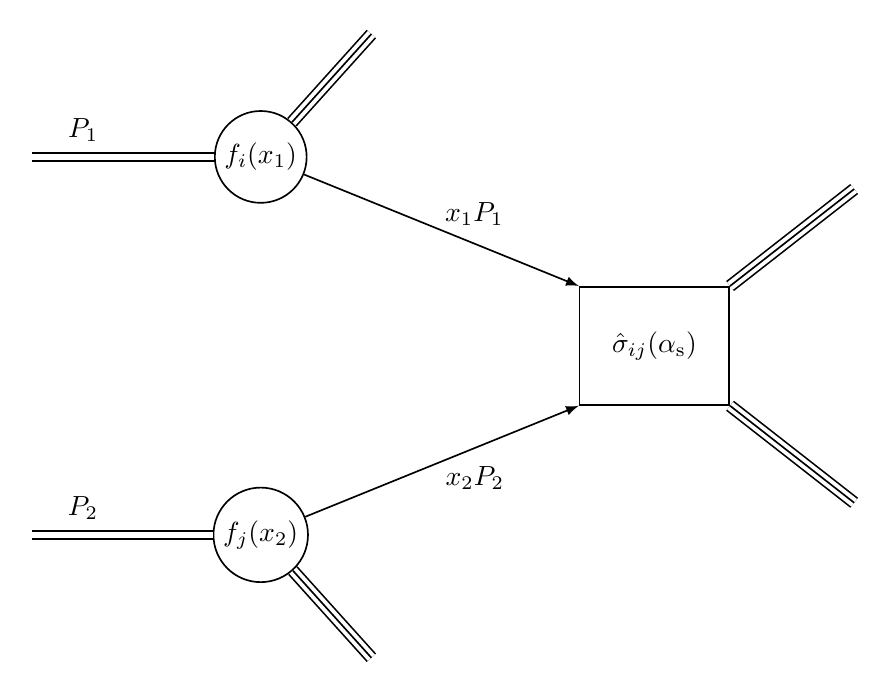
\begin{tikzpicture}[
			>=latex, line width=0.6pt,
			hadron/.style={double,double distance=2.2pt}, % incoming hadron: two lines
			triple/.style={double,double distance=3.4pt}, % outer pair of a three-line leg
		]
		% --- parton distributions and the hard-scattering blob
		\node[draw,circle,inner sep=2pt] (p1) at (0, 2.4) {$f_i(x_1)$};
		\node[draw,circle,inner sep=2pt] (p2) at (0,-2.4) {$f_j(x_2)$};
		\node[draw,minimum width=1.9cm,minimum height=1.5cm,inner sep=2pt]
		(sig) at (5.0,0) {$\hat{\sigma}_{ij}(\alpha_{\rm s})$};

		% --- endpoints of the beam remnants and the outgoing partons
		\path (p1) ++(48:2.1) coordinate (rem1);
		\path (p2) ++(-48:2.1) coordinate (rem2);
		\path (sig.north east) ++(38:2.0) coordinate (out1);
		\path (sig.south east) ++(-38:2.0) coordinate (out2);

		% --- incoming hadrons
		\draw[hadron] (-2.9, 2.4) -- (p1) node[pos=0.28,above=2pt] {$P_1$};
		\draw[hadron] (-2.9,-2.4) -- (p2) node[pos=0.28,above=2pt] {$P_2$};

		% --- three-line legs: beam remnants and outgoing partons
		\foreach \s/\e in {p1/rem1, p2/rem2, sig.north east/out1, sig.south east/out2}{
				\draw[triple] (\s) -- (\e);
				\draw (\s) -- (\e); % middle line
			}

		% --- the two partons entering the hard scattering
		\draw[->] (p1) -- (sig.north west) node[pos=0.62,above=3pt] {$x_1P_1$};
		\draw[->] (p2) -- (sig.south west) node[pos=0.62,below=3pt] {$x_2P_2$};
	\end{tikzpicture}%
}

% ---------------------------------------------------------------------------
% Leading-order 2 -> 2 partonic diagrams for jet production (tab:jetdiagrams).
% Incoming partons enter from the left, outgoing partons leave to the right.
% \jetdiagw and \jetdiagh are the half-width and half-height of every diagram,
% so the whole set is drawn on one common scale; change them to rescale the
% entire table at once.  Naming: trailing T/U/S = t-, u-, s-channel,
% X = the four-gluon contact term.
% ---------------------------------------------------------------------------
\def\jetdiagw{1.00} % half-width  of a 2->2 diagram
\def\jetdiagh{0.48} % half-height of a 2->2 diagram

% t-channel gluon exchange between two quark lines.
% Args: #1 = lower-line flavour label, #2 = upper-line flavour label.
% Used for both q q' -> q q' (distinct labels) and q q -> q q (same label).
\newcommand{\diagqqpT}[2]{%
	\begin{tikzpicture}[baseline=0, thick]
		\begin{feynman}
			\vertex (v1) at (0,-\jetdiagh);
			\vertex (v2) at (0, \jetdiagh);
			\vertex (i1) at (-\jetdiagw,-\jetdiagh) {\(#1\)};
			\vertex (o1) at ( \jetdiagw,-\jetdiagh) {\(#1\)};
			\vertex (i2) at (-\jetdiagw, \jetdiagh) {\(#2\)};
			\vertex (o2) at ( \jetdiagw, \jetdiagh) {\(#2\)};
			\diagram* {
				(i1) -- [fermion] (v1) -- [fermion] (o1),
				(i2) -- [fermion] (v2) -- [fermion] (o2),
				(v1) -- [gluon] (v2),
			};
		\end{feynman}
	\end{tikzpicture}%
}

% u-channel partner of the above: identical quarks, so the two outgoing legs
% are interchanged and the final-state lines cross.  Arg: #1 = flavour label.
\newcommand{\diagqqU}[1]{%
	\begin{tikzpicture}[baseline=0, thick]
		\begin{feynman}
			\vertex (v1) at (-0.35,-\jetdiagh);
			\vertex (v2) at (-0.35, \jetdiagh);
			\vertex (i1) at (-\jetdiagw,-\jetdiagh) {\(#1\)};
			\vertex (i2) at (-\jetdiagw, \jetdiagh) {\(#1\)};
			\vertex (o1) at ( \jetdiagw, \jetdiagh) {\(#1\)};
			\vertex (o2) at ( \jetdiagw,-\jetdiagh) {\(#1\)};
			\diagram* {
				(i1) -- [fermion] (v1) -- [fermion] (o1),
				(i2) -- [fermion] (v2) -- [fermion] (o2),
				(v1) -- [gluon] (v2),
			};
		\end{feynman}
	\end{tikzpicture}%
}

% t-channel gluon exchange between a quark line (top, left to right) and an
% antiquark line (bottom, right to left).
% Args: #1 = quark flavour, #2 = antiquark flavour (bar is supplied here).
% Covers q qbar' -> q qbar' and the t-channel of q qbar -> q qbar.
\newcommand{\diagqqbpT}[2]{%
	\begin{tikzpicture}[baseline=0, thick]
		\begin{feynman}
			\vertex (v1) at (0,-\jetdiagh);
			\vertex (v2) at (0, \jetdiagh);
			\vertex (i1) at (-\jetdiagw,-\jetdiagh) {\(\bar{#2}\)};
			\vertex (o1) at ( \jetdiagw,-\jetdiagh) {\(\bar{#2}\)};
			\vertex (i2) at (-\jetdiagw, \jetdiagh) {\(#1\)};
			\vertex (o2) at ( \jetdiagw, \jetdiagh) {\(#1\)};
			\diagram* {
				(o1) -- [fermion] (v1) -- [fermion] (i1),
				(i2) -- [fermion] (v2) -- [fermion] (o2),
				(v1) -- [gluon] (v2),
			};
		\end{feynman}
	\end{tikzpicture}%
}

% s-channel quark-antiquark annihilation through a single gluon into a
% quark-antiquark pair.  Args: #1 = incoming flavour, #2 = outgoing flavour.
% Covers q qbar -> q' qbar' and the s-channel of q qbar -> q qbar.
\newcommand{\diagqqbAnn}[2]{%
	\begin{tikzpicture}[baseline=0, thick]
		\begin{feynman}
			\vertex (i1) at (-\jetdiagw, \jetdiagh) {\(#1\)};
			\vertex (i2) at (-\jetdiagw,-\jetdiagh) {\(\bar{#1}\)};
			\vertex (v1) at (-0.35,0);
			\vertex (v2) at ( 0.35,0);
			\vertex (o1) at ( \jetdiagw, \jetdiagh) {\(#2\)};
			\vertex (o2) at ( \jetdiagw,-\jetdiagh) {\(\bar{#2}\)};
			\diagram* {
				(i1) -- [fermion] (v1) -- [fermion] (i2),
				(v1) -- [gluon] (v2),
				(o2) -- [fermion] (v2) -- [fermion] (o1),
			};
		\end{feynman}
	\end{tikzpicture}%
}

% g g -> q qbar, s-channel through the three-gluon vertex.
\newcommand{\diagggqqS}{%
	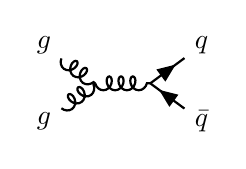
\begin{tikzpicture}[baseline=0, thick]
		\begin{feynman}
			\vertex (i1) at (-\jetdiagw, \jetdiagh) {\(g\)};
			\vertex (i2) at (-\jetdiagw,-\jetdiagh) {\(g\)};
			\vertex (v1) at (-0.35,0);
			\vertex (v2) at ( 0.35,0);
			\vertex (o1) at ( \jetdiagw, \jetdiagh) {\(q\)};
			\vertex (o2) at ( \jetdiagw,-\jetdiagh) {\(\bar{q}\)};
			\diagram* {
				(i1) -- [gluon] (v1),
				(i2) -- [gluon] (v1),
				(v1) -- [gluon] (v2),
				(o2) -- [fermion] (v2) -- [fermion] (o1),
			};
		\end{feynman}
	\end{tikzpicture}%
}

% g g -> q qbar, t-channel quark exchange.
\newcommand{\diagggqqT}{%
	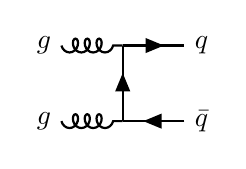
\begin{tikzpicture}[baseline=0, thick]
		\begin{feynman}
			\vertex (i1) at (-\jetdiagw, \jetdiagh) {\(g\)};
			\vertex (i2) at (-\jetdiagw,-\jetdiagh) {\(g\)};
			\vertex (v1) at (0, \jetdiagh);
			\vertex (v2) at (0,-\jetdiagh);
			\vertex (o1) at ( \jetdiagw, \jetdiagh) {\(q\)};
			\vertex (o2) at ( \jetdiagw,-\jetdiagh) {\(\bar{q}\)};
			\diagram* {
				(i1) -- [gluon] (v1),
				(i2) -- [gluon] (v2),
				(o2) -- [fermion] (v2),
				(v2) -- [fermion] (v1),
				(v1) -- [fermion] (o1),
			};
		\end{feynman}
	\end{tikzpicture}%
}

% g g -> q qbar, u-channel: the outgoing quark and antiquark are interchanged.
\newcommand{\diagggqqU}{%
	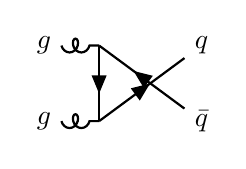
\begin{tikzpicture}[baseline=0, thick]
		\begin{feynman}
			\vertex (i1) at (-\jetdiagw, \jetdiagh) {\(g\)};
			\vertex (i2) at (-\jetdiagw,-\jetdiagh) {\(g\)};
			\vertex (v1) at (-0.30, \jetdiagh);
			\vertex (v2) at (-0.30,-\jetdiagh);
			\vertex (o1) at ( \jetdiagw, \jetdiagh) {\(q\)};
			\vertex (o2) at ( \jetdiagw,-\jetdiagh) {\(\bar{q}\)};
			\diagram* {
				(i1) -- [gluon] (v1),
				(i2) -- [gluon] (v2),
				(o2) -- [fermion] (v1),
				(v1) -- [fermion] (v2),
				(v2) -- [fermion] (o1),
			};
		\end{feynman}
	\end{tikzpicture}%
}

% q g -> q g, s-channel quark exchange.
\newcommand{\diagqgS}{%
	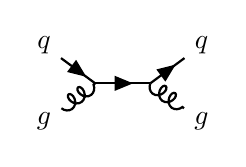
\begin{tikzpicture}[baseline=0, thick]
		\begin{feynman}
			\vertex (i1) at (-\jetdiagw, \jetdiagh) {\(q\)};
			\vertex (i2) at (-\jetdiagw,-\jetdiagh) {\(g\)};
			\vertex (v1) at (-0.35,0);
			\vertex (v2) at ( 0.35,0);
			\vertex (o1) at ( \jetdiagw, \jetdiagh) {\(q\)};
			\vertex (o2) at ( \jetdiagw,-\jetdiagh) {\(g\)};
			\diagram* {
				(i1) -- [fermion] (v1),
				(i2) -- [gluon] (v1),
				(v1) -- [fermion] (v2),
				(v2) -- [fermion] (o1),
				(v2) -- [gluon] (o2),
			};
		\end{feynman}
	\end{tikzpicture}%
}

% q g -> q g, t-channel gluon exchange.
\newcommand{\diagqgT}{%
	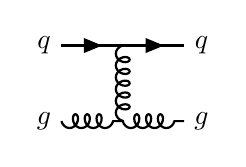
\begin{tikzpicture}[baseline=0, thick]
		\begin{feynman}
			\vertex (v1) at (0, \jetdiagh);
			\vertex (v2) at (0,-\jetdiagh);
			\vertex (i1) at (-\jetdiagw, \jetdiagh) {\(q\)};
			\vertex (o1) at ( \jetdiagw, \jetdiagh) {\(q\)};
			\vertex (i2) at (-\jetdiagw,-\jetdiagh) {\(g\)};
			\vertex (o2) at ( \jetdiagw,-\jetdiagh) {\(g\)};
			\diagram* {
				(i1) -- [fermion] (v1) -- [fermion] (o1),
				(i2) -- [gluon] (v2) -- [gluon] (o2),
				(v1) -- [gluon] (v2),
			};
		\end{feynman}
	\end{tikzpicture}%
}

% q g -> q g, u-channel quark exchange: the outgoing quark and gluon are
% interchanged relative to the t-channel diagram.
\newcommand{\diagqgU}{%
	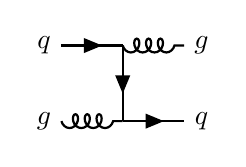
\begin{tikzpicture}[baseline=0, thick]
		\begin{feynman}
			\vertex (v1) at (0, \jetdiagh);
			\vertex (v2) at (0,-\jetdiagh);
			\vertex (i1) at (-\jetdiagw, \jetdiagh) {\(q\)};
			\vertex (o1) at ( \jetdiagw, \jetdiagh) {\(g\)};
			\vertex (i2) at (-\jetdiagw,-\jetdiagh) {\(g\)};
			\vertex (o2) at ( \jetdiagw,-\jetdiagh) {\(q\)};
			\diagram* {
				(i1) -- [fermion] (v1),
				(v1) -- [gluon] (o1),
				(i2) -- [gluon] (v2),
				(v1) -- [fermion] (v2),
				(v2) -- [fermion] (o2),
			};
		\end{feynman}
	\end{tikzpicture}%
}

% q qbar -> g g, s-channel annihilation through the three-gluon vertex.
\newcommand{\diagqqbS}{%
	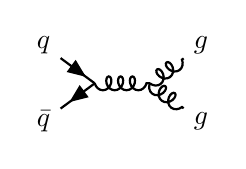
\begin{tikzpicture}[baseline=0, thick]
		\begin{feynman}
			\vertex (i1) at (-\jetdiagw, \jetdiagh) {\(q\)};
			\vertex (i2) at (-\jetdiagw,-\jetdiagh) {\(\bar{q}\)};
			\vertex (v1) at (-0.35,0);
			\vertex (v2) at ( 0.35,0);
			\vertex (o1) at ( \jetdiagw, \jetdiagh) {\(g\)};
			\vertex (o2) at ( \jetdiagw,-\jetdiagh) {\(g\)};
			\diagram* {
				(i1) -- [fermion] (v1) -- [fermion] (i2),
				(v1) -- [gluon] (v2),
				(v2) -- [gluon] (o1),
				(v2) -- [gluon] (o2),
			};
		\end{feynman}
	\end{tikzpicture}%
}

% q qbar -> g g, t-channel quark exchange.
\newcommand{\diagqqbT}{%
	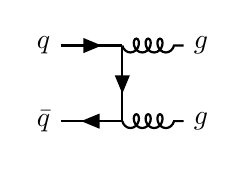
\begin{tikzpicture}[baseline=0, thick]
		\begin{feynman}
			\vertex (i1) at (-\jetdiagw, \jetdiagh) {\(q\)};
			\vertex (i2) at (-\jetdiagw,-\jetdiagh) {\(\bar{q}\)};
			\vertex (v1) at (0, \jetdiagh);
			\vertex (v2) at (0,-\jetdiagh);
			\vertex (o1) at ( \jetdiagw, \jetdiagh) {\(g\)};
			\vertex (o2) at ( \jetdiagw,-\jetdiagh) {\(g\)};
			\diagram* {
				(i1) -- [fermion] (v1),
				(v1) -- [fermion] (v2),
				(v2) -- [fermion] (i2),
				(v1) -- [gluon] (o1),
				(v2) -- [gluon] (o2),
			};
		\end{feynman}
	\end{tikzpicture}%
}

% q qbar -> g g, u-channel: as above with the two outgoing gluons interchanged.
\newcommand{\diagqqbU}{%
	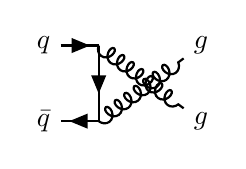
\begin{tikzpicture}[baseline=0, thick]
		\begin{feynman}
			\vertex (i1) at (-\jetdiagw, \jetdiagh) {\(q\)};
			\vertex (i2) at (-\jetdiagw,-\jetdiagh) {\(\bar{q}\)};
			\vertex (v1) at (-0.30, \jetdiagh);
			\vertex (v2) at (-0.30,-\jetdiagh);
			\vertex (o1) at ( \jetdiagw, \jetdiagh) {\(g\)};
			\vertex (o2) at ( \jetdiagw,-\jetdiagh) {\(g\)};
			\diagram* {
				(i1) -- [fermion] (v1),
				(v1) -- [fermion] (v2),
				(v2) -- [fermion] (i2),
				(v1) -- [gluon] (o2),
				(v2) -- [gluon] (o1),
			};
		\end{feynman}
	\end{tikzpicture}%
}

% g g -> g g, s-channel through two three-gluon vertices.
\newcommand{\diagggS}{%
	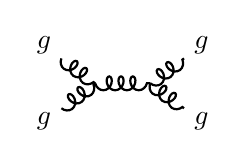
\begin{tikzpicture}[baseline=0, thick]
		\begin{feynman}
			\vertex (i1) at (-\jetdiagw, \jetdiagh) {\(g\)};
			\vertex (i2) at (-\jetdiagw,-\jetdiagh) {\(g\)};
			\vertex (v1) at (-0.35,0);
			\vertex (v2) at ( 0.35,0);
			\vertex (o1) at ( \jetdiagw, \jetdiagh) {\(g\)};
			\vertex (o2) at ( \jetdiagw,-\jetdiagh) {\(g\)};
			\diagram* {
				(i1) -- [gluon] (v1),
				(i2) -- [gluon] (v1),
				(v1) -- [gluon] (v2),
				(v2) -- [gluon] (o1),
				(v2) -- [gluon] (o2),
			};
		\end{feynman}
	\end{tikzpicture}%
}

% g g -> g g, t-channel gluon exchange.
\newcommand{\diagggT}{%
	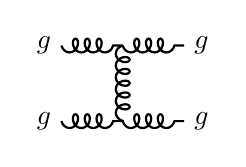
\begin{tikzpicture}[baseline=0, thick]
		\begin{feynman}
			\vertex (v1) at (0, \jetdiagh);
			\vertex (v2) at (0,-\jetdiagh);
			\vertex (i1) at (-\jetdiagw, \jetdiagh) {\(g\)};
			\vertex (o1) at ( \jetdiagw, \jetdiagh) {\(g\)};
			\vertex (i2) at (-\jetdiagw,-\jetdiagh) {\(g\)};
			\vertex (o2) at ( \jetdiagw,-\jetdiagh) {\(g\)};
			\diagram* {
				(i1) -- [gluon] (v1) -- [gluon] (o1),
				(i2) -- [gluon] (v2) -- [gluon] (o2),
				(v1) -- [gluon] (v2),
			};
		\end{feynman}
	\end{tikzpicture}%
}

% g g -> g g, u-channel: the two outgoing gluons are interchanged.
\newcommand{\diagggU}{%
	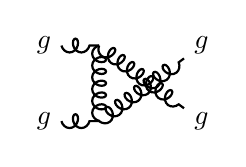
\begin{tikzpicture}[baseline=0, thick]
		\begin{feynman}
			\vertex (v1) at (-0.30, \jetdiagh);
			\vertex (v2) at (-0.30,-\jetdiagh);
			\vertex (i1) at (-\jetdiagw, \jetdiagh) {\(g\)};
			\vertex (o1) at ( \jetdiagw, \jetdiagh) {\(g\)};
			\vertex (i2) at (-\jetdiagw,-\jetdiagh) {\(g\)};
			\vertex (o2) at ( \jetdiagw,-\jetdiagh) {\(g\)};
			\diagram* {
				(i1) -- [gluon] (v1),
				(v1) -- [gluon] (o2),
				(i2) -- [gluon] (v2),
				(v2) -- [gluon] (o1),
				(v1) -- [gluon] (v2),
			};
		\end{feynman}
	\end{tikzpicture}%
}

% g g -> g g, the four-gluon contact term (cf. the four-gluon vertex of
% tab:qcdrules), redrawn here on the common 2->2 scale.
\newcommand{\diagggX}{%
	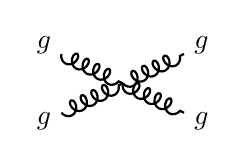
\begin{tikzpicture}[baseline=0, thick]
		\begin{feynman}
			\vertex (v) at (0,0);
			\vertex (i1) at (-\jetdiagw, \jetdiagh) {\(g\)};
			\vertex (i2) at (-\jetdiagw,-\jetdiagh) {\(g\)};
			\vertex (o1) at ( \jetdiagw, \jetdiagh) {\(g\)};
			\vertex (o2) at ( \jetdiagw,-\jetdiagh) {\(g\)};
			\diagram* {
				(i1) -- [gluon] (v),
				(i2) -- [gluon] (v),
				(v) -- [gluon] (o1),
				(v) -- [gluon] (o2),
			};
		\end{feynman}
	\end{tikzpicture}%
}

% Macro for 4-point vertices
% Args: #1=top-left style, #2=top-left label, #3=bottom-left style, #4=bottom-left label,
%       #5=top-right style, #6=top-right label, #7=bottom-right style, #8=bottom-right label
\newcommand{\fourvertex}[8]{%
	\begin{tikzpicture}[baseline=0, thick]
		\begin{feynman}
			\vertex [circle, fill=black, minimum size=3.5pt, inner sep=0pt] (v) at (0,0) {};
			\vertex (i1) at (135:1.5) {\(#2\)};
			\vertex (i2) at (225:1.5) {\(#4\)};
			\vertex (o1) at (45:1.5) {\(#6\)};
			\vertex (o2) at (-45:1.5) {\(#8\)};
			\diagram* {
				(i1) -- [#1] (v),
				(i2) -- [#3] (v),
				(v) -- [#5] (o1),
				(v) -- [#7] (o2),
			};
		\end{feynman}
	\end{tikzpicture}%
}

\def\splitw{0.95} % half-width  of a 1->2 splitting diagram
\def\splith{0.62} % half-height of a 1->2 splitting diagram
\newcommand{\splitvertex}[9]{%
	\begin{tikzpicture}[baseline=0, thick]
		\begin{feynman}
			\vertex [circle, fill=black, minimum size=3.5pt, inner sep=0pt] (v) at (0,0) {};
			\vertex (p) at (-\splitw, 0)        {\(#2\)};
			\vertex (u) at ( \splitw,  \splith) {\(#5\)};
			\vertex (l) at ( \splitw, -\splith) {\(#8\)};
			\diagram* {
				(p) -- [#1, edge label'=\(#3\)] (v),
				(v) -- [#4, edge label=\(#6\)]  (u),
				(v) -- [#7, edge label'=\(#9\)] (l),
			};
		\end{feynman}
	\end{tikzpicture}%
}
\newcommand\drawDiJetInVacuum{
   % \begin{tikzpicture}
        \begin{feynhand}
            \vertex (a)  at (-4, -1); 
            \vertex (b)  at (-4, 1) ; 
            \vertex (a1) at (-3.5, -0.5); 
            \vertex (a1_isr) at (-3, -0.5);
            \vertex (b1) at (-3.5, 0.5); 
            \vertex (b1_isr) at (-4, 0.5);
            \propag [plain] (a) to (a1);
            \propag [plain] (b) to (b1);
            \propag [bos] (a1) to (a1_isr);
            \propag [bos] (b1) to (b1_isr);
            \vertex (c)  at (-3, 0); 
            \vertex (d)  at (-2, 0);
            \propag [fermion] (a1) to (c);
            \propag [fermion] (c) to (b1);
            \propag [gluon] (c) to (d);
            \vertex (e) at (-1.5, -0.5); 
            \vertex (f) at (-1.5, 0.5);
            \propag [fermion] (d) to (e);
            \propag [plain] (f) to (d);
            \vertex (f0) at (-1, 1.); 
            \propag [fermion] (f0) to (f);
            \vertex (f00) at (0, 3);
            \propag [bos] (f0) to (f00);
            \vertex (f01) at (-0.5, 1.5);
            \propag [plain] (f01) to (f0);
            \vertex [NWblob] (f010) at (1.0, 2.5) {};
            \propag [fermion] (f010) to (f01);
            \vertex (f011) at (0.2, 1.5);
            \propag [gluon] (f01) to (f011);
            \propag [fermion] (f011) to (f010);
            \vertex (f1) at (-1, 0.);
            \propag [gluon] (f) to (f1);
            \vertex (f10) at (0., 0);
            \vertex (f11) at (0., .75);
            \propag [gluon] (f1) to (f10);
            \propag [gluon] (f1) to (f11);
            \vertex [NWblob] (f110) at (1., 0.5) {};
            \vertex [NWblob] (f111) at (1., 1.3) {};
            \propag [fermion] (f110) to (f11);
            \propag [fermion] (f11) to (f111);
            \propag [fermion] (f10) to (f110);
            \vertex [NWblob] (f101) at (1.0, -0.5) {};
            \propag [fermion] (f101) to (f10);
            \propag [fermion] (f111) to (f011);
            \vertex (e0) at (0, -1); 
            \vertex (ep) at (-1., -1);
            \propag [gluon] (e) to (e0);
            \propag [plain] (e) to (ep);
            \vertex [NWblob] (epp) at (1, -1.5) {};
            \vertex (ep0) at (0, -2);
            \propag [fermion] (ep) to (epp);
            \propag [bos] (ep) to (ep0);
            %\vertex (e01) at (0.5, -0.5);
            \propag [fermion] (e0) to (epp); 
            \propag [fermion] (f101) to (e0);
            \vertex [ringdot] (h10) at (1.6, 2.8) {};
            \vertex [ringdot] (h101) at (1.6, 2.4) {};
            \propag[plain] (f010) to (h10);
            \propag[plain] (f010) to (h101);
            \vertex [ringdot] (h102) at (1.8, 2.7) {};
            \propag[plain] (h101) to (h102);
            \vertex [ringdot] (h103) at (1.8, 2.3) {};
            \propag[plain] (h101) to (h103);
            \vertex [ringdot] (h11) at (1.6, 1.4) {};
            \vertex [ringdot] (h111) at (1.6, 1.0) {};	
            \propag[plain] (f111) to (h11);
            \propag[plain] (f111) to (h111);
            \vertex [ringdot] (h112) at (1.8, 1.3) {};
            \propag[plain] (h111) to (h112);
            \vertex [ringdot] (h113) at (1.8, 0.9) {};
            \propag[plain] (h111) to (h113);
            \vertex [ringdot] (h12) at (1.6, 0.6) {};
            \vertex [ringdot] (h121) at (1.6, 0.2) {};
            \propag[plain] (f110) to (h12);
            \propag[plain] (f110) to (h121);
            \vertex [ringdot] (h122) at (1.8, 0.5) {};
            \propag[plain] (h121) to (h122);
            \vertex [ringdot] (h123) at (1.8, 0.1) {};
            \propag[plain] (h121) to (h123);
            \vertex [ringdot] (h124) at (2.0, 0.6) {};
            \propag[plain] (h122) to (h124);
            \vertex [ringdot] (h125) at (2.0, 0.4) {};
            \propag[plain] (h122) to (h125);
            \vertex [ringdot] (h13) at (1.6, -0.4) {};
            \vertex [ringdot] (h131) at (1.6, -0.8) {};
            \propag[plain] (f101) to (h13);
            \propag[plain] (f101) to (h131);
            \vertex [ringdot] (h132) at (1.8, -0.7) {};
            \propag[plain] (h131) to (h132);
            \vertex [ringdot] (h134) at (1.8, -0.9) {};
            \propag[plain] (h131) to (h134);
            \vertex [ringdot] (h14) at (1.6, -1.6) {};
            \vertex [ringdot] (h141) at (1.6, -2.0) {};
            \propag[plain] (epp) to (h14);
            \propag[plain] (epp) to (h141);
            \vertex [ringdot] (h142) at (1.8, -1.8) {};
            \propag[plain] (h141) to (h142);
            \vertex [ringdot] (h144) at (1.8, -2.0) {};
            \propag[plain] (h141) to (h144);
        \end{feynhand}
                
    %\end{tikzpicture}
}

\newcommand\drawDiJetInMedium{
    \begin{feynhand}
        \vertex (a)  at (-4, -1); 
        \vertex (b)  at (-4, 1) ; 
        \vertex (a1) at (-3.5, -0.5); 
        \vertex (a1_isr) at (-3, -0.5);
        \vertex (b1) at (-3.5, 0.5); 
        \vertex (b1_isr) at (-4, 0.5);
        \propag [plain] (a) to (a1);
        \propag [plain] (b) to (b1);
        \propag [bos] (a1) to (a1_isr);
        \propag [bos] (b1) to (b1_isr);
        \vertex (c)  at (-3, 0); 
        \vertex (d)  at (-2, 0);
        \propag [fermion] (a1) to (c);
        \propag [fermion] (c) to (b1);
        \propag [gluon] (c) to (d);
        \vertex (f) at (-1.5, 0.5);
        \vertex (f0) at (-1, 1.); 
        \vertex (f1) at (-1, 0.);
        \vertex (f00) at (0, 3);
        \vertex (f01) at (-0.5, 1.5);
        \vertex (f10) at (0., 0);
        \vertex (f11) at (0., .75);
        \vertex (f011) at (0.2, 1.5);
            \vertex (f_med) at (-2.5, 3);
            \vertex (f_med0) at (-1.5, 2);
            \vertex (f_med1) at (-1., 2.5);
            \propag [fermion, red] (f_med) to (f_med0);
            \propag [fermion, red] (f_med0) to (f_med1);
            \vertex (f0_med) at (-1.4, 1.25);
            \propag [gluon, red] (f0_med) to (f_med0);
            \propag [fermion, red] (f0_med) to (f);
            \propag [fermion, red] (f0) to (f0_med);
        
        \propag [gluon] (f) to (f1);
        \propag [fermion] (f) to (d);
        \propag [plain] (f01) to (f0);
        \propag [bos] (f0) to (f00);
        
        \vertex [NWblob] (f010) at (1.0, 2.5) {};
        \propag [fermion] (f010) to (f01);
        \propag [gluon] (f01) to (f011);
        \propag [fermion] (f011) to (f010);
        
        \propag [gluon] (f1) to (f10);
        \propag [gluon] (f1) to (f11);
        \vertex [NWblob] (f110) at (1., 0.5) {};
        \vertex [NWblob] (f111) at (1., 1.3) {};
        \propag [fermion] (f110) to (f11);
        \propag [fermion] (f11) to (f111);
        \propag [fermion] (f10) to (f110);
        \vertex [NWblob] (f101) at (1.0, -0.5) {};
        \propag [fermion] (f101) to (f10);
        \propag [fermion] (f111) to (f011);
        
        
        
        
        
            \vertex (e) at (-1.5, -0.5); 
            \vertex (e_med) at (-1.8, -0.7);
            \vertex (e_med_1) at (-1.75, -1.5);
            \propag [fermion, red] (d) to (e_med);
            \propag [fermion, red] (e_med) to (e);
            \propag [gluon, red] (e_med) to (e_med_1);
        
        \vertex (e0) at (0, -1); 
        \vertex (ep) at (-1., -1);
        
        \propag [gluon] (e) to (e0);
        \propag [plain] (e) to (ep);
        \vertex [NWblob] (epp) at (1, -1.5) {};
        \vertex (ep0) at (0, -2);
        \propag [fermion] (ep) to (epp);
        \propag [bos] (ep) to (ep0);
        %\vertex (e01) at (0.5, -0.5);
        \propag [fermion] (e0) to (epp); 
        \propag [fermion] (f101) to (e0);
        \vertex [ringdot] (h10) at (1.6, 2.8) {};
        \vertex [ringdot] (h101) at (1.6, 2.4) {};
        \propag[plain] (f010) to (h10);
        \propag[plain] (f010) to (h101);
        \vertex [ringdot] (h102) at (1.8, 2.7) {};
        \propag[plain] (h101) to (h102);
        \vertex [ringdot] (h103) at (1.8, 2.3) {};
        \propag[plain] (h101) to (h103);
        \vertex [ringdot] (h11) at (1.6, 1.4) {};
        \vertex [ringdot] (h111) at (1.6, 1.0) {};	
        \propag[plain] (f111) to (h11);
        \propag[plain] (f111) to (h111);
        \vertex [ringdot] (h112) at (1.8, 1.3) {};
        \propag[plain] (h111) to (h112);
        \vertex [ringdot] (h113) at (1.8, 0.9) {};
        \propag[plain] (h111) to (h113);
        \vertex [ringdot] (h12) at (1.6, 0.6) {};
        \vertex [ringdot] (h121) at (1.6, 0.2) {};
        \propag[plain] (f110) to (h12);
        \propag[plain] (f110) to (h121);
        \vertex [ringdot] (h122) at (1.8, 0.5) {};
        \propag[plain] (h121) to (h122);
        \vertex [ringdot] (h123) at (1.8, 0.1) {};
        \propag[plain] (h121) to (h123);
        \vertex [ringdot] (h124) at (2.0, 0.6) {};
        \propag[plain] (h122) to (h124);
        \vertex [ringdot] (h125) at (2.0, 0.4) {};
        \propag[plain] (h122) to (h125);
        \vertex [ringdot] (h13) at (1.6, -0.4) {};
        \vertex [ringdot] (h131) at (1.6, -0.8) {};
        \propag[plain] (f101) to (h13);
        \propag[plain] (f101) to (h131);
        \vertex [ringdot] (h132) at (1.8, -0.7) {};
        \propag[plain] (h131) to (h132);
        \vertex [ringdot] (h134) at (1.8, -0.9) {};
        \propag[plain] (h131) to (h134);
        \vertex [ringdot] (h14) at (1.6, -1.6) {};
        \vertex [ringdot] (h141) at (1.6, -2.0) {};
        \propag[plain] (epp) to (h14);
        \propag[plain] (epp) to (h141);
        \vertex [ringdot] (h142) at (1.8, -1.8) {};
        \propag[plain] (h141) to (h142);
        \vertex [ringdot] (h144) at (1.8, -2.0) {};
        \propag[plain] (h141) to (h144);
    \end{feynhand}
    \draw[fill=violet!20, rounded corners, opacity=0.2] (-2.0, 3.5) rectangle (0.6, -2.5) node at (-1.0, 3.) {Medium};
    
        \node[fill=orange!50] at (-2, -1.8) {Inelastic collisions};
        \node[fill=orange!50] at (-3, 1.8) {Elastic collisions};
} % \drawDiJetInVacuum, \drawDiJetInMedium (from the ICNFP-2024 talk)

\setbeamerfont{footnote}{size=\tiny}

% short reference at the bottom left of a frame, e.g. \refnote{STAR, PRC 109 (2024) 044909}
\newcommand{\refnote}[1]{%
	\begin{textblock*}{0.8\paperwidth}(0.03\paperwidth, 0.885\paperheight)
		{\tiny\color{gray}#1}
	\end{textblock*}}

% Slide copies of \threevertex / \fourvertex (defines/TikzDiagrams.tex), scaled down, with the
% vertex remembered as coordinate #1 and its coupling #2 drawn in red on overlays \couplingspec
\newcommand{\couplingspec}{3-}
\newcommand{\sthreevertex}[8]{%
	\begin{tikzpicture}[baseline=0, thick, scale=0.55, remember picture]
		\begin{feynman}
			\vertex [circle, fill=black, minimum size=3.5pt, inner sep=0pt] (v) at (0,0) {};
			\vertex (i1) at (240:1.5) {\(#4\)};
			\vertex (i2) at (120:1.5) {\(#6\)};
			\vertex [circle, fill=black, minimum size=2.5pt, inner sep=0pt] (o) at (1.5,0) {};
			\diagram* {
				(i1) -- [#3] (v) -- [#5] (i2),
				(v) -- [#7, edge label'=\(#8\)] (o)
			};
		\end{feynman}
		\coordinate (#1) at (0,0);
		\node[anchor=east, text=PrimaryColor, font=\footnotesize, inner sep=1pt, visible on=<\couplingspec>] at (-0.2,0) {\(#2\)};
	\end{tikzpicture}%
}
\newcommand{\sfourvertex}[7]{% #1 name, #2 coupling, #3 line style of all four legs, #4-#7 labels
	\begin{tikzpicture}[baseline=0, thick, scale=0.55, remember picture]
		\begin{feynman}
			\vertex [circle, fill=black, minimum size=3.5pt, inner sep=0pt] (v) at (0,0) {};
			\vertex (i1) at (135:1.5) {\(#4\)};
			\vertex (i2) at (225:1.5) {\(#5\)};
			\vertex (o1) at (45:1.5) {\(#6\)};
			\vertex (o2) at (-45:1.5) {\(#7\)};
			\diagram* {
				(i1) -- [#3] (v),
				(i2) -- [#3] (v),
				(v) -- [#3] (o1),
				(v) -- [#3] (o2),
			};
		\end{feynman}
		\coordinate (#1) at (0,0);
		\node[anchor=west, text=PrimaryColor, font=\footnotesize, inner sep=1pt, visible on=<\couplingspec>] at (0.3,0) {\(#2\)};
	\end{tikzpicture}%
}

% show a TikZ scope only on some overlays while keeping its space: \begin{scope}[visible on=<2->]
\tikzset{
	invisible/.style={opacity=0, text opacity=0},
	visible on/.style={alt={#1{}{invisible}}},
	alt/.code args={<#1>#2#3}{\alt<#1>{\pgfkeysalso{#2}}{\pgfkeysalso{#3}}},
}

% MultiFold flow boxes (from slides/preliminary_request)
\tikzset{
	databox/.style={rounded corners, draw=red!70!black,    fill=red!10,    line width=0.9pt, align=center, inner sep=5pt, minimum width=3.2cm, minimum height=0.95cm, font=\small},
	recobox/.style={rounded corners, draw=blue!70!black,   fill=blue!10,   line width=0.9pt, align=center, inner sep=5pt, minimum width=3.2cm, minimum height=0.95cm, font=\small},
	genbox/.style ={rounded corners, draw=green!55!black,  fill=green!12,  line width=0.9pt, align=center, inner sep=5pt, minimum width=3.2cm, minimum height=0.95cm, font=\small},
	steparr/.style={-{Stealth[length=2.6mm]}, line width=1.1pt},
	proparr/.style={-{Stealth[length=2.6mm]}, line width=1.1pt, densely dashed},
	flowlbl/.style={font=\scriptsize, align=left, text width=3.6cm},
}

% SoftDrop schematic palette (Fig. softDropSchematic)
\definecolor{sdnavy}{RGB}{0,76,127}
\definecolor{sdblue}{RGB}{0,159,254}
\definecolor{sdlight}{RGB}{187,204,230}
\definecolor{sdcyan}{RGB}{85,190,255}

\newcommand{\lam}[1]{\ensuremath{\lambda^{\kappa=1}_{#1}}\xspace}
\newcommand{\Rg}{\ensuremath{R_\mathrm{g}}\xspace}
\newcommand{\zg}{\ensuremath{z_\mathrm{g}}\xspace}
\newcommand{\PYsix}{PYTHIA\mbox{-}6\xspace}
\newcommand{\PYeight}{PYTHIA\mbox{-}8\xspace}
\newcommand{\HWseven}{HERWIG\mbox{-}7\xspace}

\title{Spacetime evolution of jets}
\subtitle{with the STAR experiment}
\author{Tanmay Pani}
\supervisors[Advisor:]{Prof. Sevil Salur}
\institute{Department of Physics and Astronomy, Rutgers University}
\date{October 2026}
\setTitleLogoLeft{figures/logos/Rutgers}
\setTitleLogoRight{figures/logos/STAR}
\setLogo{figures/logos/STAR}

\begin{document}

%======================================================================
\begin{frame}
	\titlepage
\end{frame}

%\begin{frame}{The voyage}
%	\begin{columns}[T]
%		\begin{column}{0.58\textwidth}
%			\begin{enumerate}
%				\item \textbf{Setting out:} QCD, jets and the quark-gluon plasma
%				\item \textbf{The ship:} RHIC and the STAR detector
%				\item \textbf{Path length:} jet-hadron correlations relative to the event plane in Au+Au
%				\item \textbf{Substructure in the medium:} angularities of hard-core jets in Au+Au
%				\item \alert{\textbf{Homeward:} inclusive and groomed angularities in \(p+p\) with unbinned unfolding}
%				\item \textbf{Ithaca:} summary and outlook
%			\end{enumerate}
%		\end{column}
%		\begin{column}{0.38\textwidth}
%			\small
%			Two questions:
%			\begin{itemize}
%				\item Does jet quenching depend on the path length through the medium?
%				\item How is the energy of a jet distributed in angle?
%			\end{itemize}
%			\vspace{2mm}
%			\emph{Because soft gluon radiation is ordered in angle, the second is a question about the history of the parton shower.}
%		\end{column}
%	\end{columns}
%\end{frame}

%======================================================================
\section{QCD, jets and the QGP}
\begin{frame}{The Standard Model}
	\centering
	\begin{tikzpicture}[
		callout/.style={draw=PrimaryColor, fill=white, rounded corners=3pt, line width=0.8pt,
				text width=3.3cm, align=left, inner sep=4pt, font=\scriptsize, execute at begin node={\hyphenpenalty=10000\exhyphenpenalty=10000}},
		pointer/.style={-{Stealth[length=2mm]}, PrimaryColor, line width=0.8pt}]
		\node[anchor=south west, inner sep=0] (sm) at (0,0) {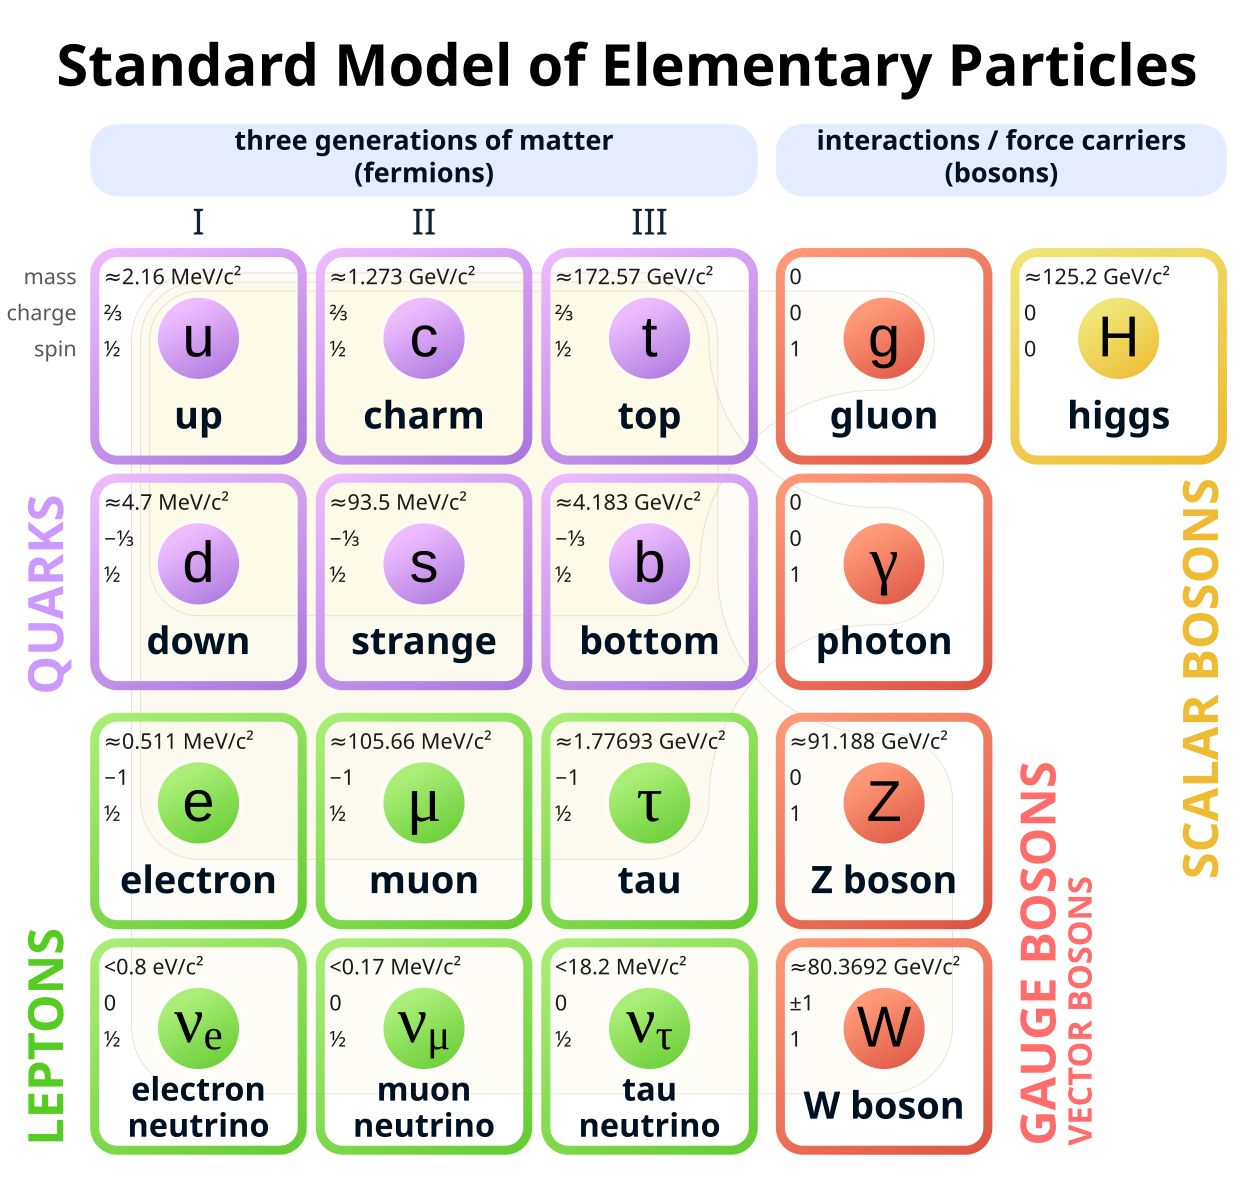
\includegraphics[height=0.7\textheight]{SM.png}};
		% unit square on the image (1254 x 1200 px)
		\begin{scope}[x={(sm.south east)}, y={(sm.north west)}]
			% fermions, left
			\node[callout, anchor=east] (q) at (-0.04,0.66) {\textbf{Quarks}: electric + \alert{color} charge; EM, weak, strong};
			\node[callout, anchor=east] (l) at (-0.04,0.22) {\textbf{Leptons}: no color; \(e, \mu, \tau\): EM + weak; \(\nu\): weak only};
			\draw[pointer] (q.east) -- (0.06,0.61);
			\draw[pointer] (l.east) -- (0.06,0.22);
			% bosons, right
			\node[callout, anchor=west] (h) at (1.04,0.84) {\textbf{Higgs} \(H\): mass};
			\node[callout, anchor=west] (g) at (1.04,0.55) {\textbf{Gluon} \(g\): strong; couples to quarks + \alert{itself}};
			\node[callout, anchor=west] (a) at (1.04,0.36) {\textbf{Photon} \(\gamma\): EM; couples to electric charge};
			\node[callout, anchor=west] (w) at (1.04,0.14) {\(\boldsymbol{W^\pm}\), \(\boldsymbol{Z}\): weak; \(W\) changes flavor (\(d \to u\))};
			\draw[pointer] (h.west) -- (0.98,0.76);
			\draw[pointer] (g.west) -- (0.79,0.625);
			\draw[pointer] (a.west) -- (0.79,0.50);
			\draw[pointer] (w.west) -- (0.79,0.22);
		\end{scope}
	\end{tikzpicture}\\[1mm]
	{\scriptsize Works from atoms to TeV --- but no gravity, dark matter, \(\nu\) masses}
	\only<2>{%
		\begin{tikzpicture}[remember picture, overlay]
			\fill[white, opacity=0.75] (current page.south west) rectangle (current page.north east);
			\node[draw=PrimaryColor, fill=white, rounded corners=4pt, line width=1.2pt, inner sep=10pt,
				font=\Large\bfseries, text=PrimaryColor, drop shadow] at (current page.center)
			{But what is meant by ``coupling'' ??};
		\end{tikzpicture}}
\end{frame}

\begin{frame}{Interaction vertices and couplings}
	\centering
	\begin{tabular}{
		>{\centering\arraybackslash}m{2.25cm}
		>{\centering\arraybackslash}m{2.25cm}
		>{\centering\arraybackslash}m{2.25cm}
		>{\centering\arraybackslash}m{2.25cm}
		}
		\multicolumn{1}{c}{\vhead{Electromagnetic}}                                                                  & \multicolumn{3}{l}{\vhead{Strong}} \\
		\sthreevertex{vEM}{e}{fermion}{X^{+|-}}{fermion}{X^{-|+}}{photon}{\gamma}                                    &
		\sthreevertex{vQG}{g_s}{fermion}{q}{fermion}{q}{gluon}{g}                                                    &
		\sthreevertex{vGGG}{g_s}{gluon}{g}{gluon}{g}{gluon}{g}                                                       &
		\sfourvertex{vGGGG}{g_s^2}{gluon}{g}{g}{g}{g}
		\\[-0.1cm]
		\multicolumn{3}{l}{\vhead{Weak}}                                                                             &                                    \\
		\sthreevertex{vWL}{g_W}{fermion}{\nu_e \mid \nu_\mu \mid \nu_\tau}{fermion}{e \mid \mu \mid \tau}{photon}{W} &
		\sthreevertex{vWQ}{g_W}{fermion}{d/s/b}{fermion}{u/c/t}{photon}{W}                                           &
		\sthreevertex{vZ}{g_Z}{fermion}{f}{fermion}{f}{photon}{Z}                                                    &
		\\[-0.1cm]
		\multicolumn{2}{l}{\vhead{Electroweak}}                                                                      & \multicolumn{2}{l}{\vhead{Higgs}}  \\
		\sthreevertex{vEW}{g_W}{photon}{Z/\gamma}{photon}{W}{photon}{W}                                              &
		\sfourvertex{vEWW}{g_W^2}{photon}{W}{W}{W|Z/\gamma}{W|Z/\gamma}                                              &
		\sthreevertex{vH}{m/v}{fermion}{m}{fermion}{m}{scalar}{H}                                                    &
		\sfourvertex{vHH}{m_B^2/v^2}{scalar}{H}{H}{m_B}{m_B}
	\end{tabular}
	\begin{tikzpicture}[remember picture, overlay,
		callout/.style={draw=PrimaryColor, fill=white, rounded corners=3pt, line width=0.8pt,
				text width=2.6cm, align=left, inner sep=4pt, font=\scriptsize, execute at begin node={\hyphenpenalty=10000\exhyphenpenalty=10000}},
		pointer/.style={-{Stealth[length=2mm]}, PrimaryColor, line width=0.8pt}]
		% left: what a vertex and a coupling are
		\node<2->[callout, anchor=west] (cv) at ([xshift=0.25cm, yshift=1.6cm]current page.west) {\textbf{Vertex}: mediator emitted / absorbed};
		\draw<2>[pointer] (cv.east) -- ([xshift=-2pt]vEM);
		\node<3->[callout, anchor=west] (cc) at ([xshift=0.25cm, yshift=-0.6cm]current page.west) {\textbf{Coupling} = vertex strength};
		\draw<3->[pointer] (cc.east) -- ([xshift=-20pt]vWL);
		% empty Weak-row cell: what the couplings do to a cross section
		\node<4->[callout, text width=4cm, anchor=south west] (ca) at ([xshift=1.0cm, yshift=-0.15cm]vZ) {Each vertex: \(\times g\) in amplitude \(\Rightarrow\) \(\sigma \propto \alpha^n\), \(\alpha = g^2/4\pi\)};
		\node<5->[callout, text width=4cm, anchor=north west] (cs) at ([xshift=1.0cm, yshift=-0.25cm]vZ) {More emissions / loops \(\to\) series in \(\alpha\): needs \(\alpha\) small\\QED \(\alpha \approx 1/137\) \checkmark{} --- QCD \(\alpha_s\)\,?};
	\end{tikzpicture}
\end{frame}
\begin{frame}{Quantum chromodynamics}
	\begin{columns}[c]
		\begin{column}{0.39\textwidth}
			\begin{itemize}
				\item Quarks, gluons: \emph{color} charge
				\item<2-> \textbf{Asymptotic freedom:} \(\alpha_s \downarrow\) as \(Q \uparrow\) \(\Rightarrow\) pQCD
				\item<3-> \textbf{Confinement:} \(\alpha_s\) large at low \(Q\) \(\Rightarrow\) only hadrons seen
				\item<4-> Hard-scattered partons \(\to\) collimated hadron sprays: \alert{jets}
			\end{itemize}
		\end{column}
		\begin{column}{0.59\textwidth}
			\centering
			\only<1>{%
				\begin{tikzpicture}
					\node[anchor=south west, inner sep=0] (sm) at (0,0) {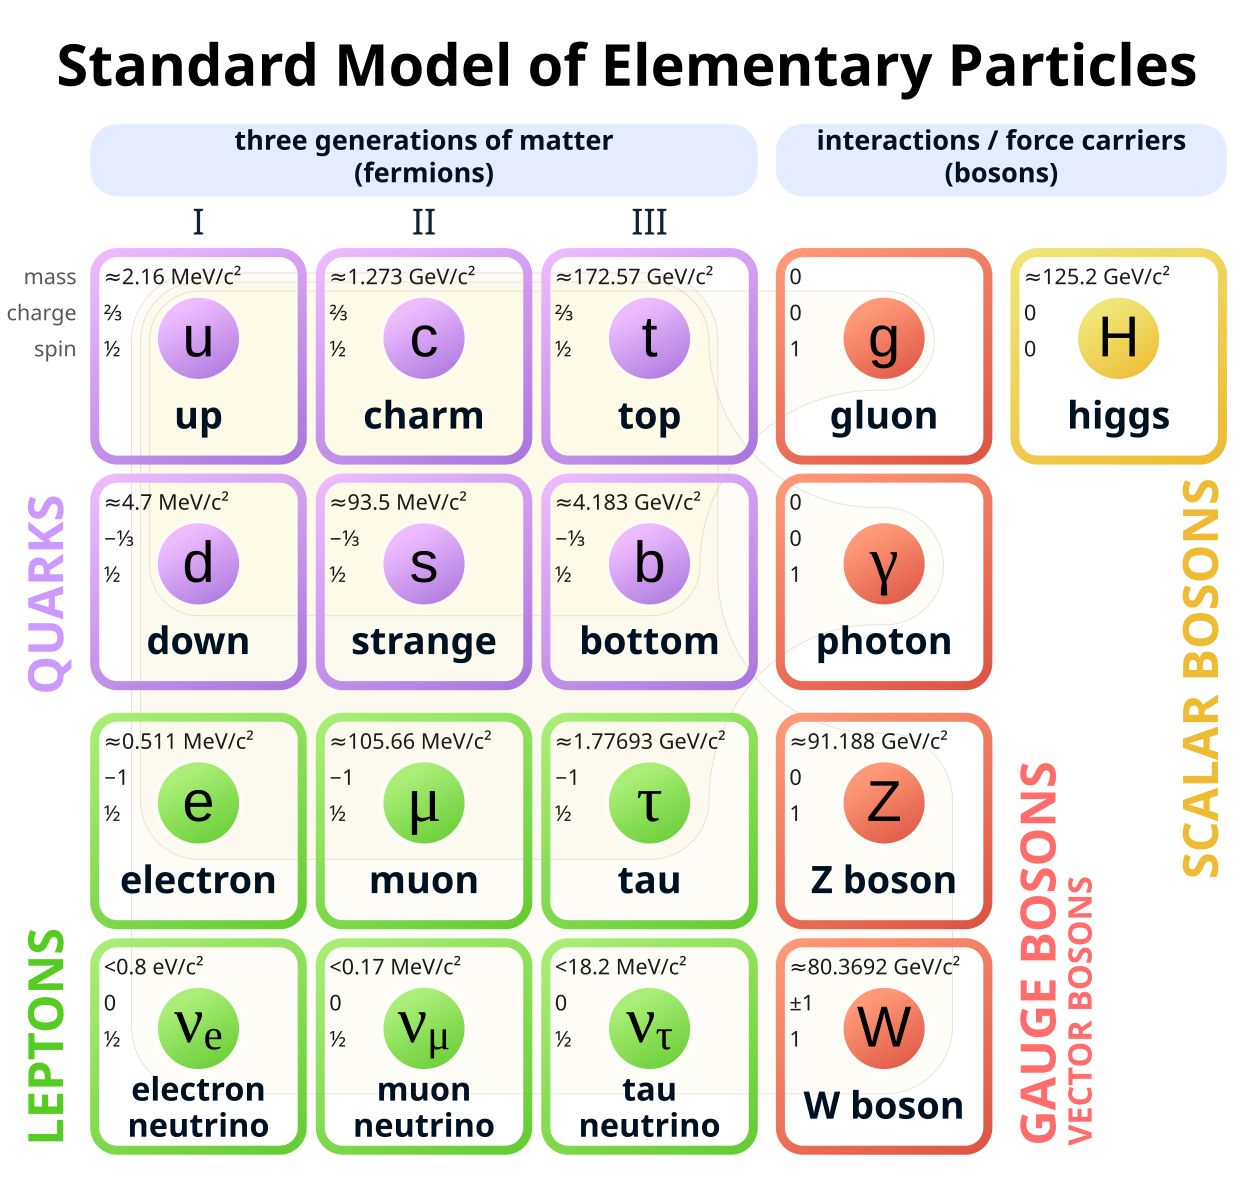
\includegraphics[width=\linewidth,height=0.78\textheight,keepaspectratio]{SM.png}};
					% unit square on the image; corners from pixel coordinates of the 1254 x 1200 image
					\begin{scope}[x={(sm.south east)}, y={(sm.north west)}]
						\draw[red, line width=2pt, rounded corners=4pt]
						(0.0654,0.8017) -- (0.7967,0.8017) -- (0.7967,0.6067) -- (0.6093,0.6067) -- (0.6093,0.4167) -- (0.0654,0.4167) -- cycle;
					\end{scope}
				\end{tikzpicture}}%
			\only<2-3>{%
				\begin{tikzpicture}
					\node[anchor=south west, inner sep=0] (as) at (0,0) {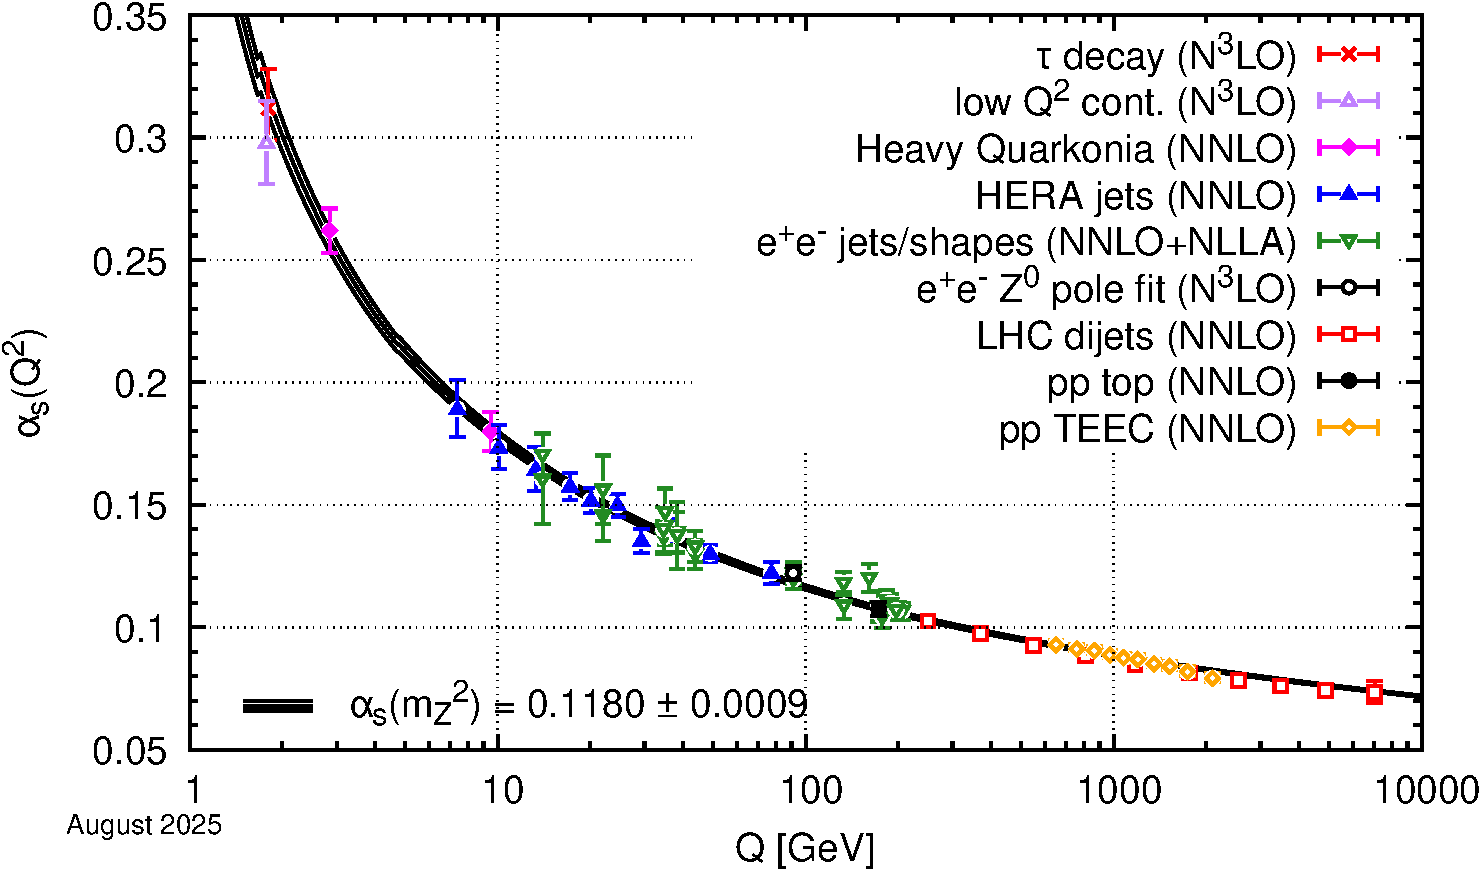
\includegraphics[width=\linewidth,height=0.78\textheight,keepaspectratio]{alphas-v-Q-2025-cropped.pdf}};
					% unit square on the plot (986 x 585 px render)
					\begin{scope}[x={(as.south east)}, y={(as.north west)}]
						% asymptotic freedom: alpha_s small at high Q
						\draw<2->[red, line width=1.5pt] (0.78,0.25) ellipse [x radius=0.17, y radius=0.085];
						% confinement: alpha_s grows at low Q
						\draw<3->[red, line width=1.5pt] (0.19,0.83) ellipse [x radius=0.075, y radius=0.17];
					\end{scope}
				\end{tikzpicture}%
				\refnote{PDG, Review of Particle Physics (2025)}}
			\only<4>{%
				\begin{tabular}{@{}>{\centering\arraybackslash}m{3mm}@{\hspace{2pt}}>{\centering\arraybackslash}m{0.85\linewidth}@{}}
					\rotatebox{90}{\scriptsize\(qq \to qq\)} & 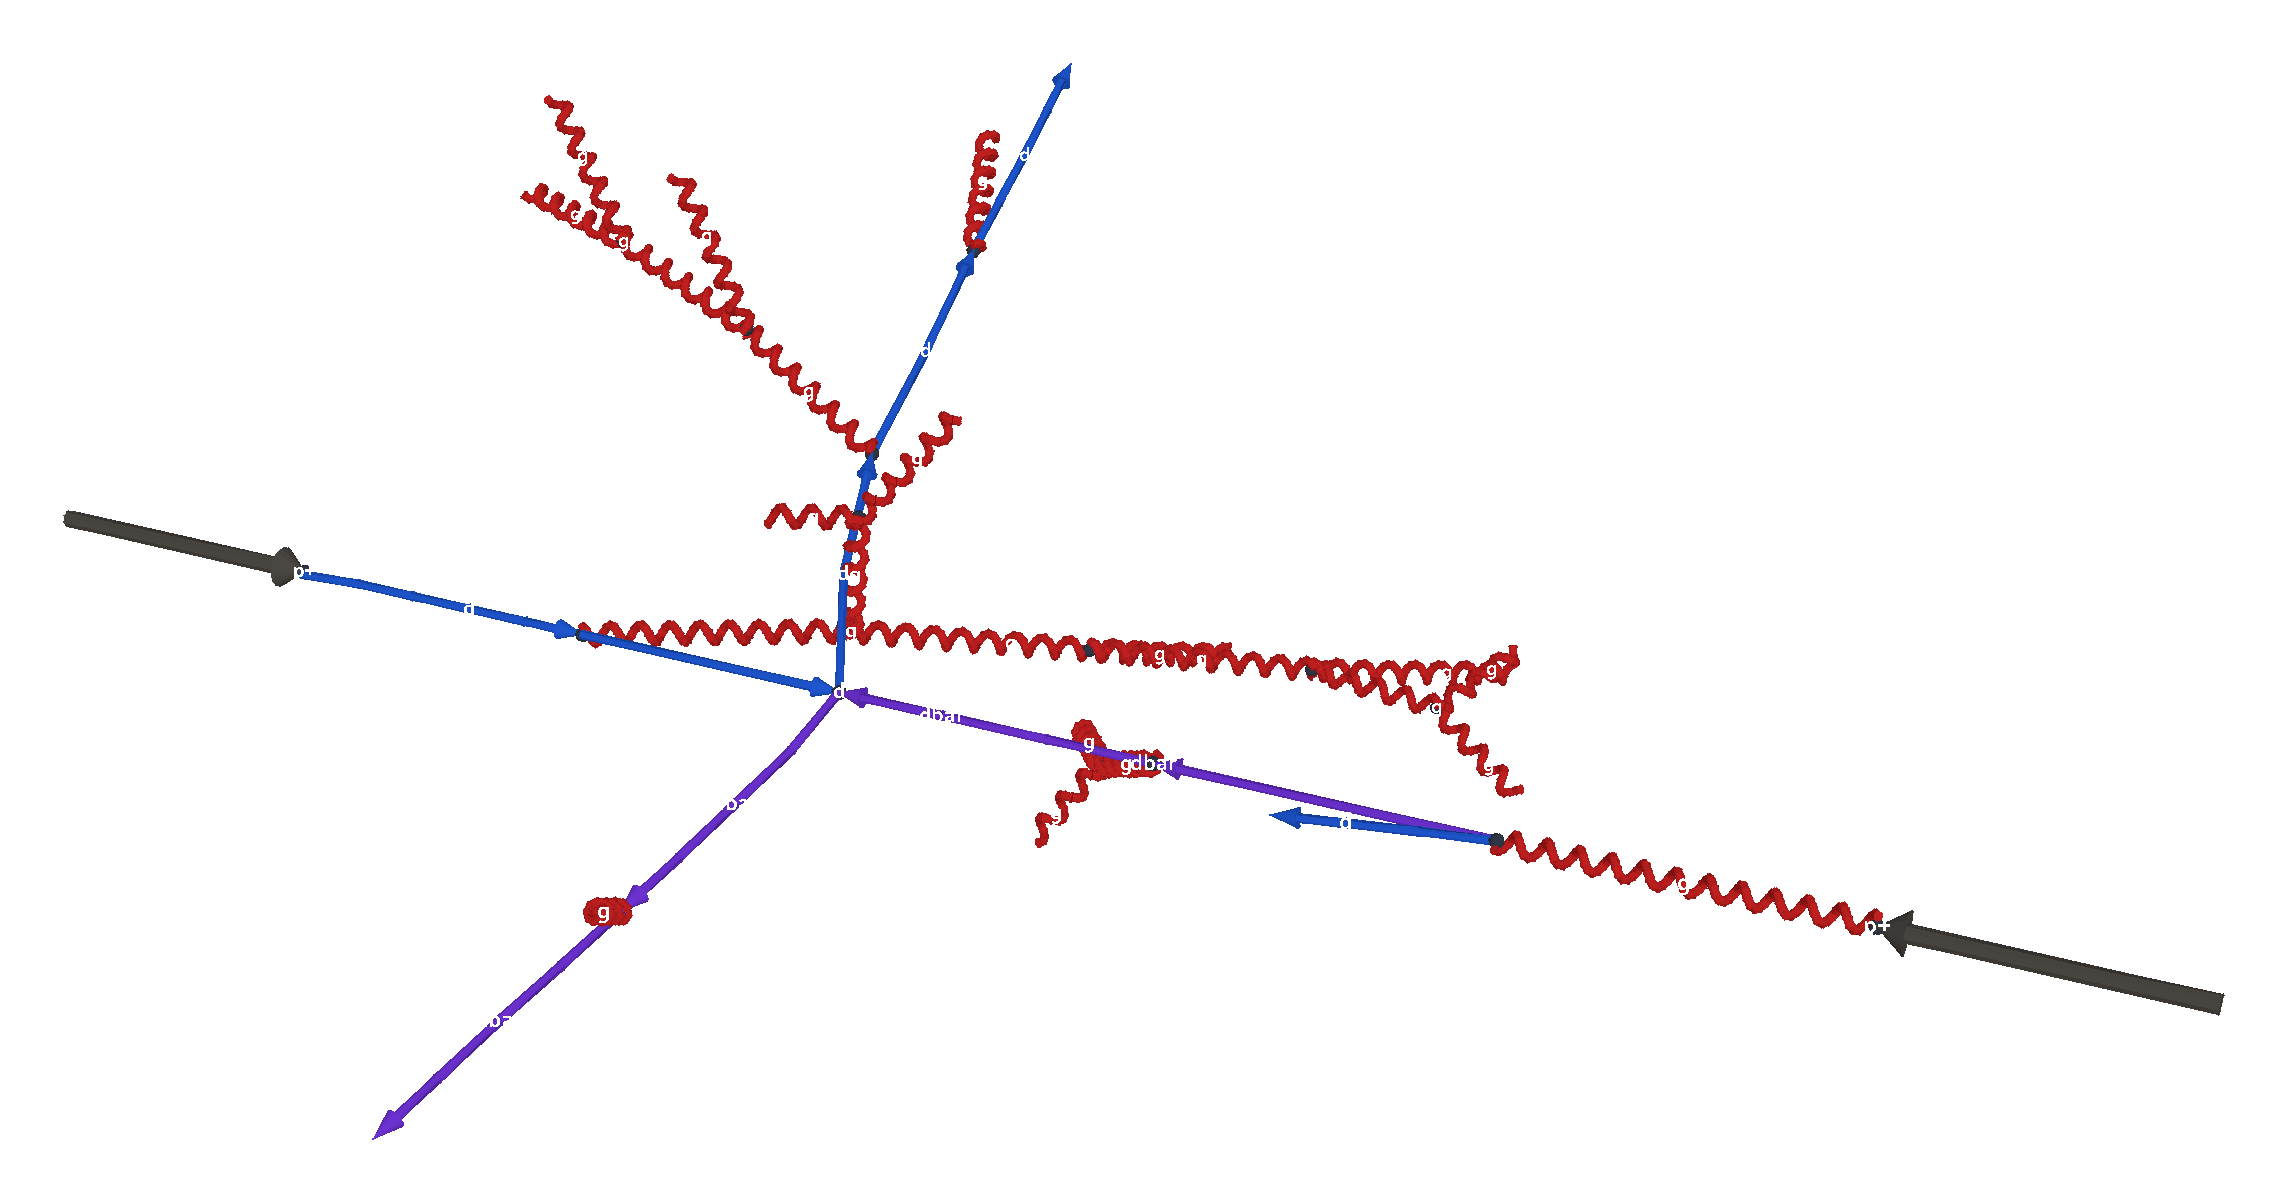
\includegraphics[height=0.24\textheight]{partonShower/qq2qq_noHadr.pdf} \\
					\rotatebox{90}{\scriptsize\(qg \to qg\)} & 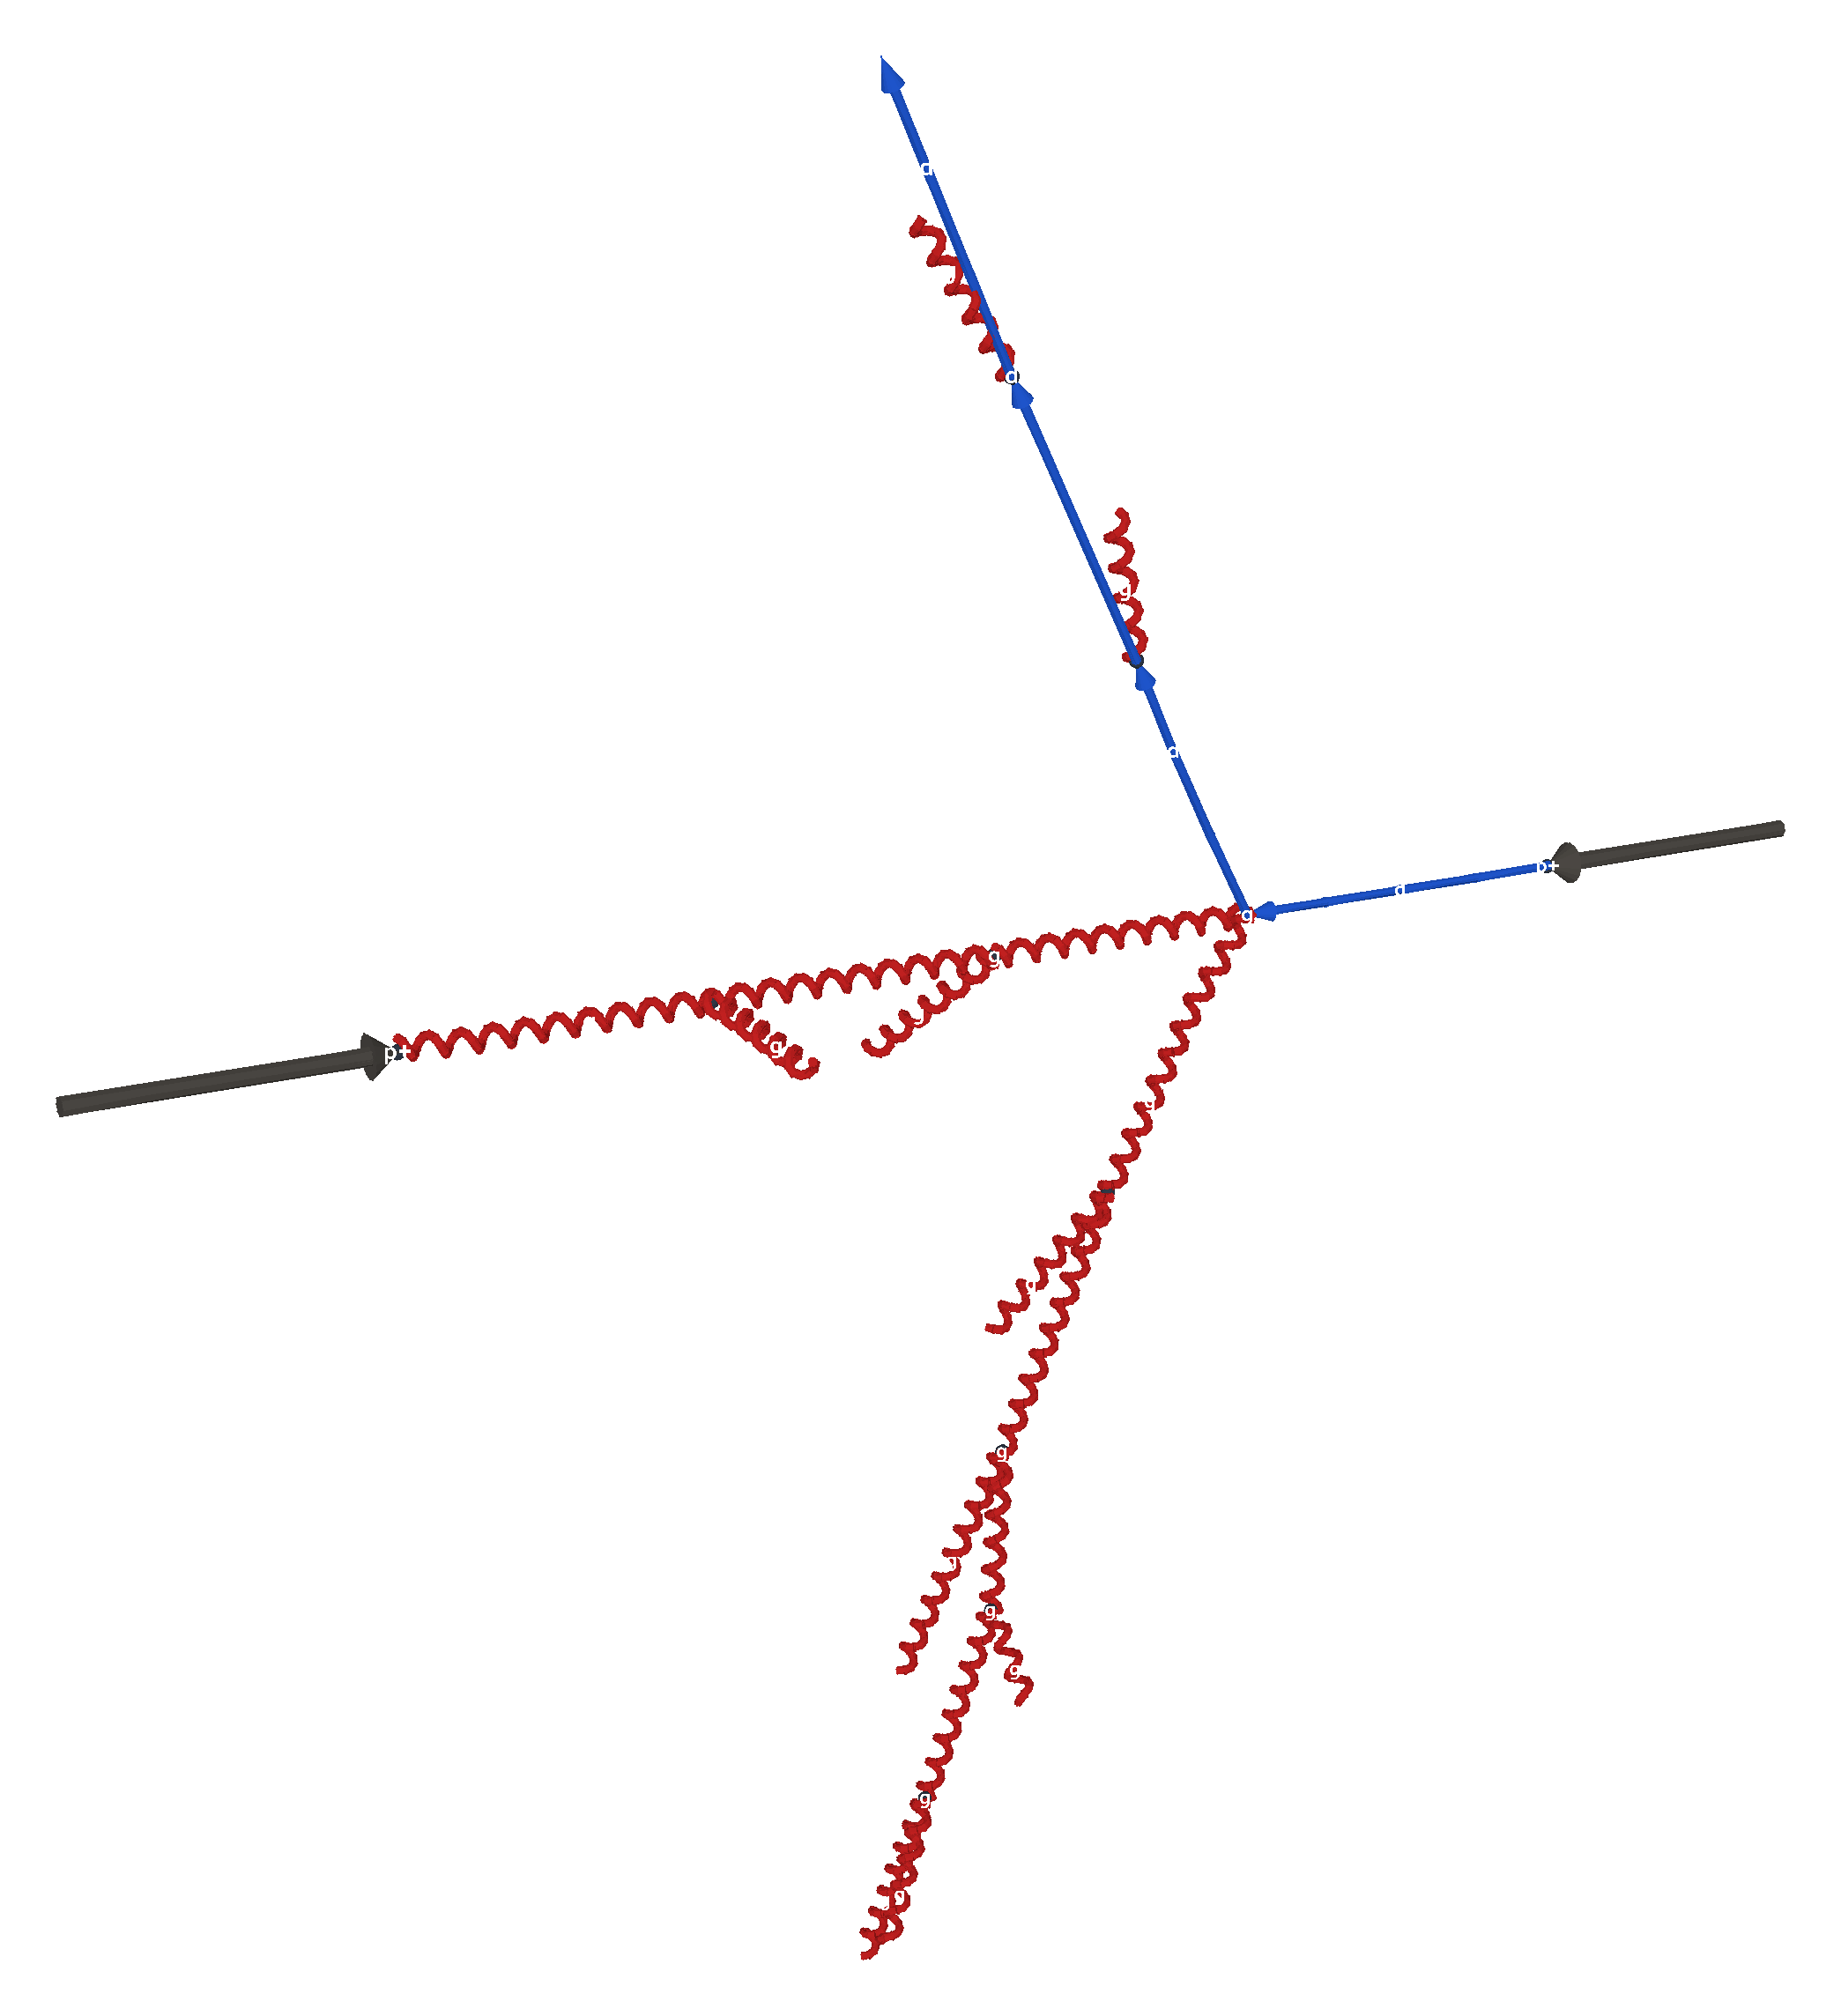
\includegraphics[height=0.24\textheight]{partonShower/qg2qg_noHadr.pdf} \\
					\rotatebox{90}{\scriptsize\(gg \to gg\)} & 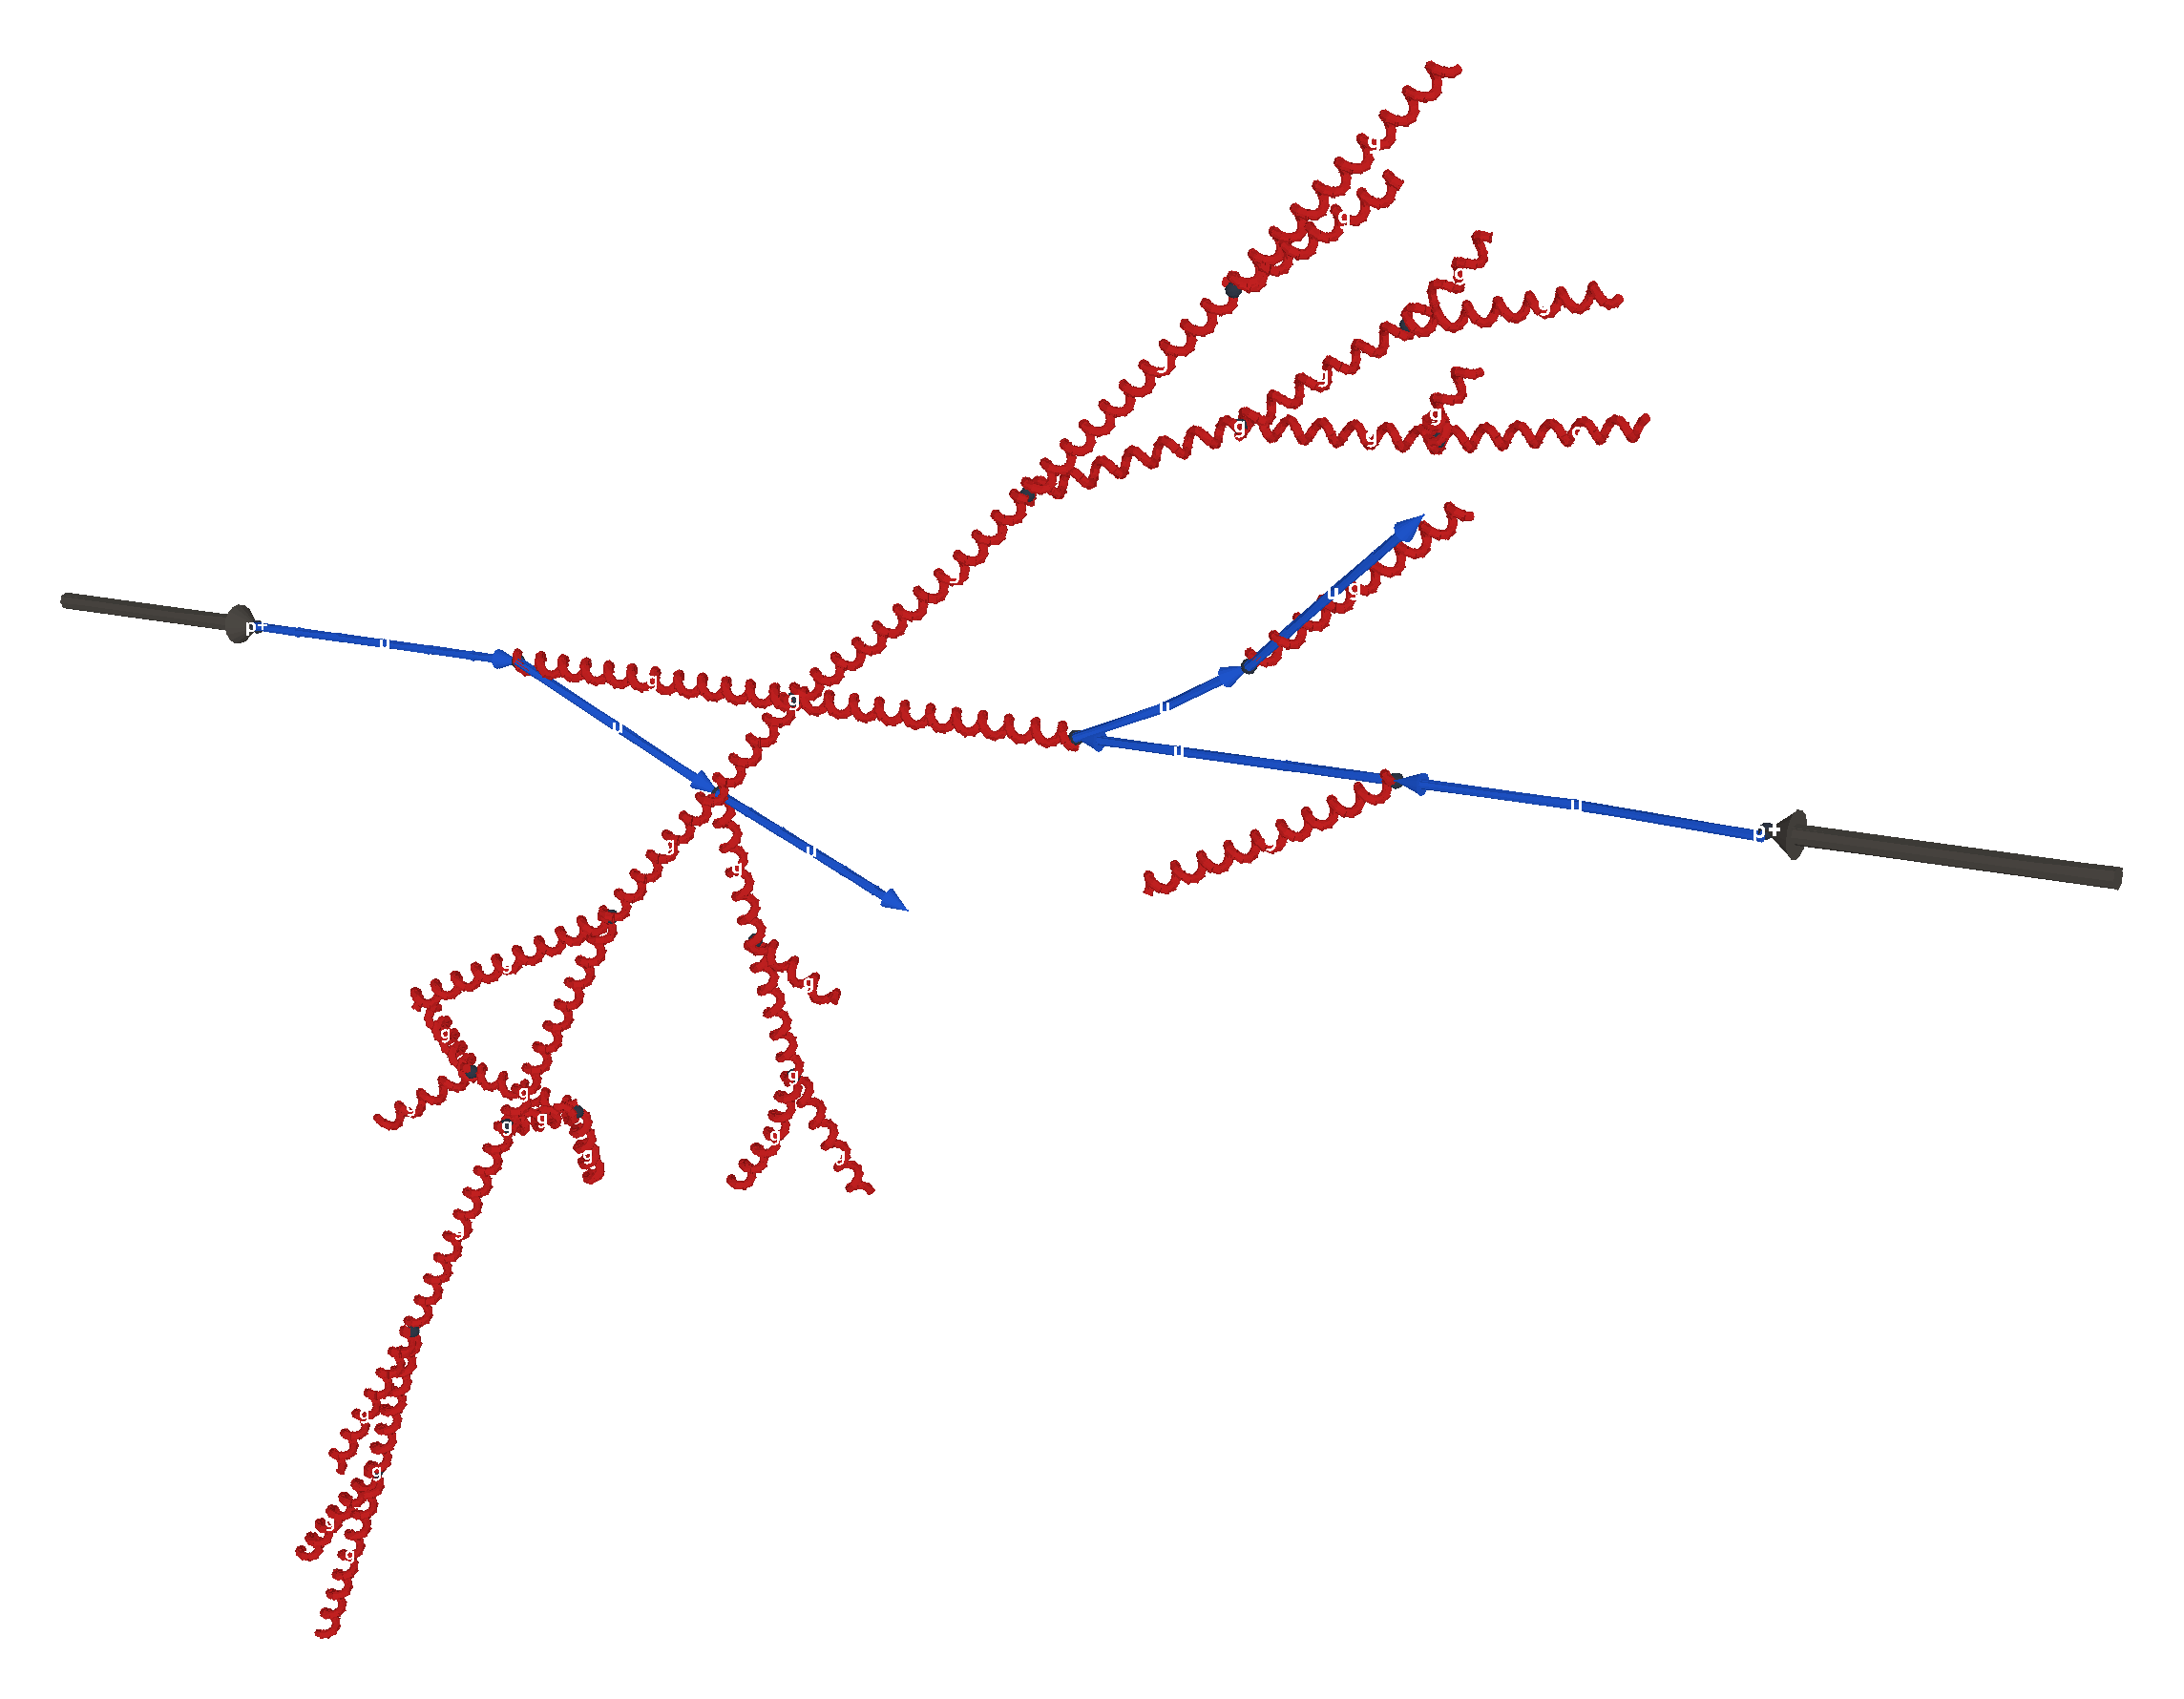
\includegraphics[height=0.24\textheight]{partonShower/gg2gg_noHadr.pdf}
				\end{tabular}}
		\end{column}
	\end{columns}

\end{frame}

\begin{frame}{From partons to hadrons}
	\centering
	\begin{tikzpicture}[
		callout/.style={draw=PrimaryColor, fill=white, rounded corners=3pt, line width=0.8pt,
				text width=3.5cm, align=left, inner sep=4pt, font=\scriptsize, execute at begin node={\hyphenpenalty=10000\exhyphenpenalty=10000}},
		pointer/.style={-{Stealth[length=2mm]}, PrimaryColor, line width=0.8pt}]
		% one qg -> qg event: shower (clicks 1-2), then hadrons (click 3 on)
		\node[inner sep=0, visible on=<1-2>] (sh) at (0,0) {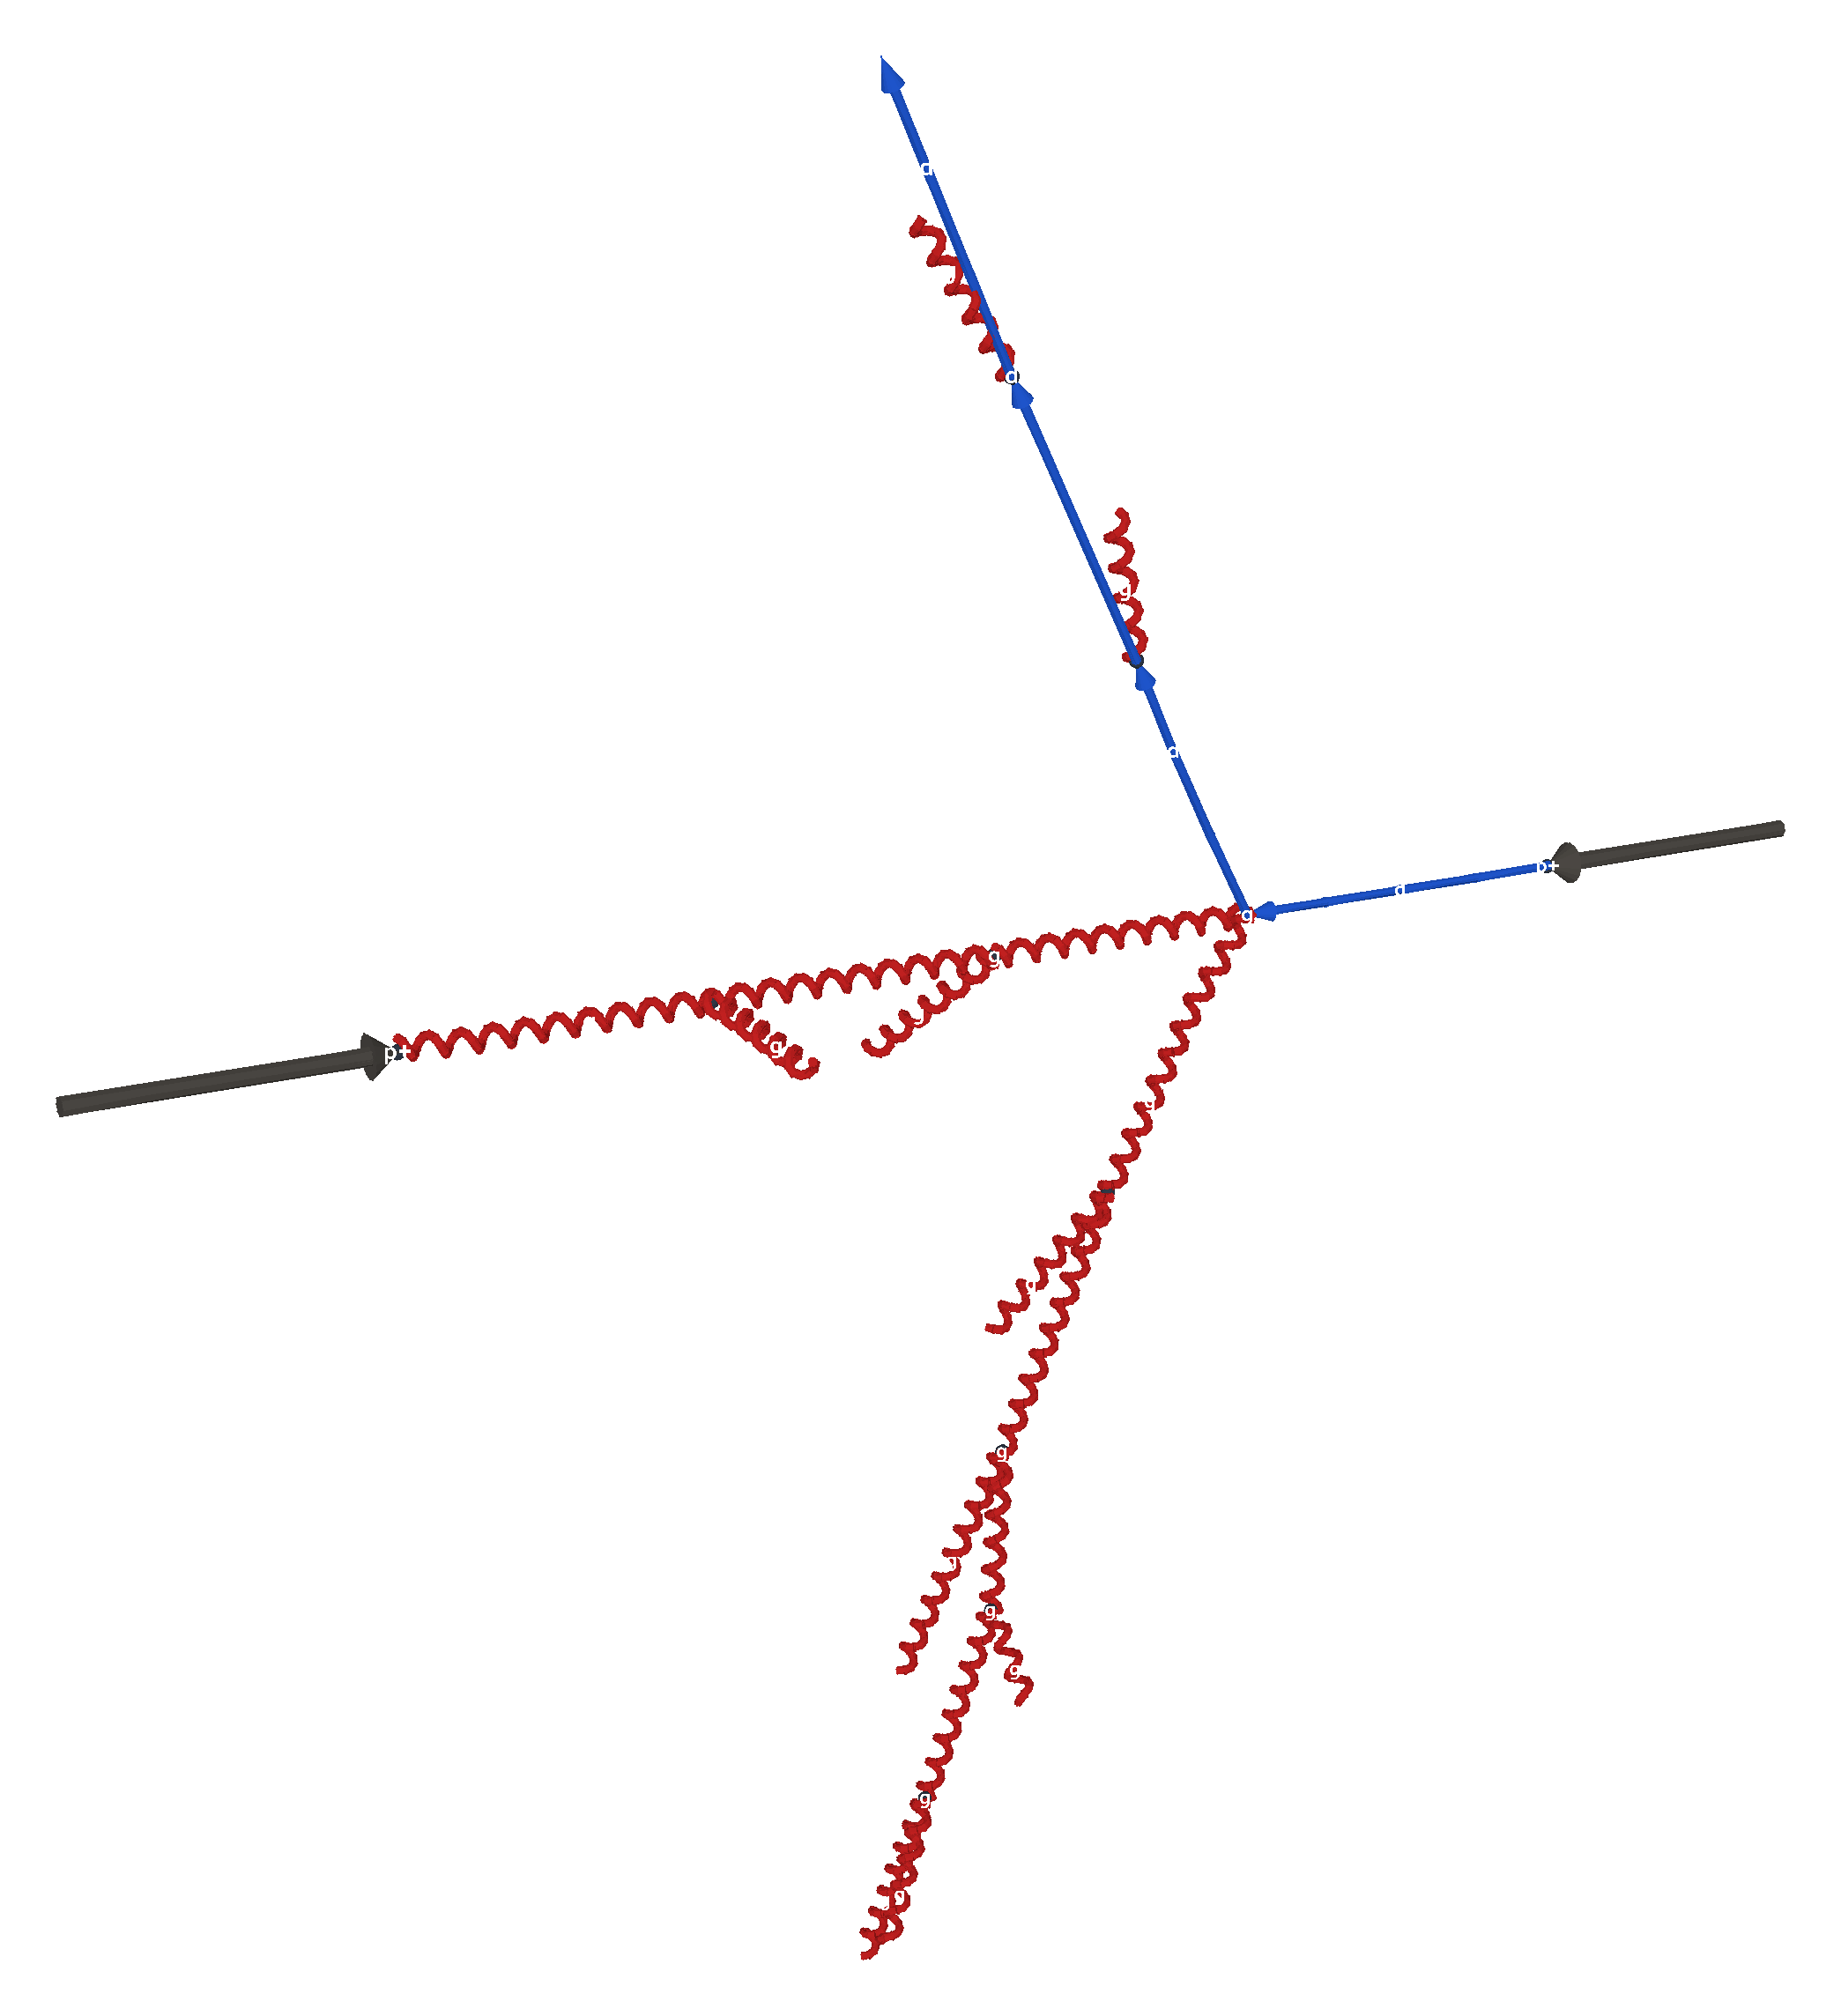
\includegraphics[height=0.66\textheight]{partonShower/qg2qg_noHadr.pdf}};
		\node[inner sep=0, visible on=<3->] (hd) at (0,0) {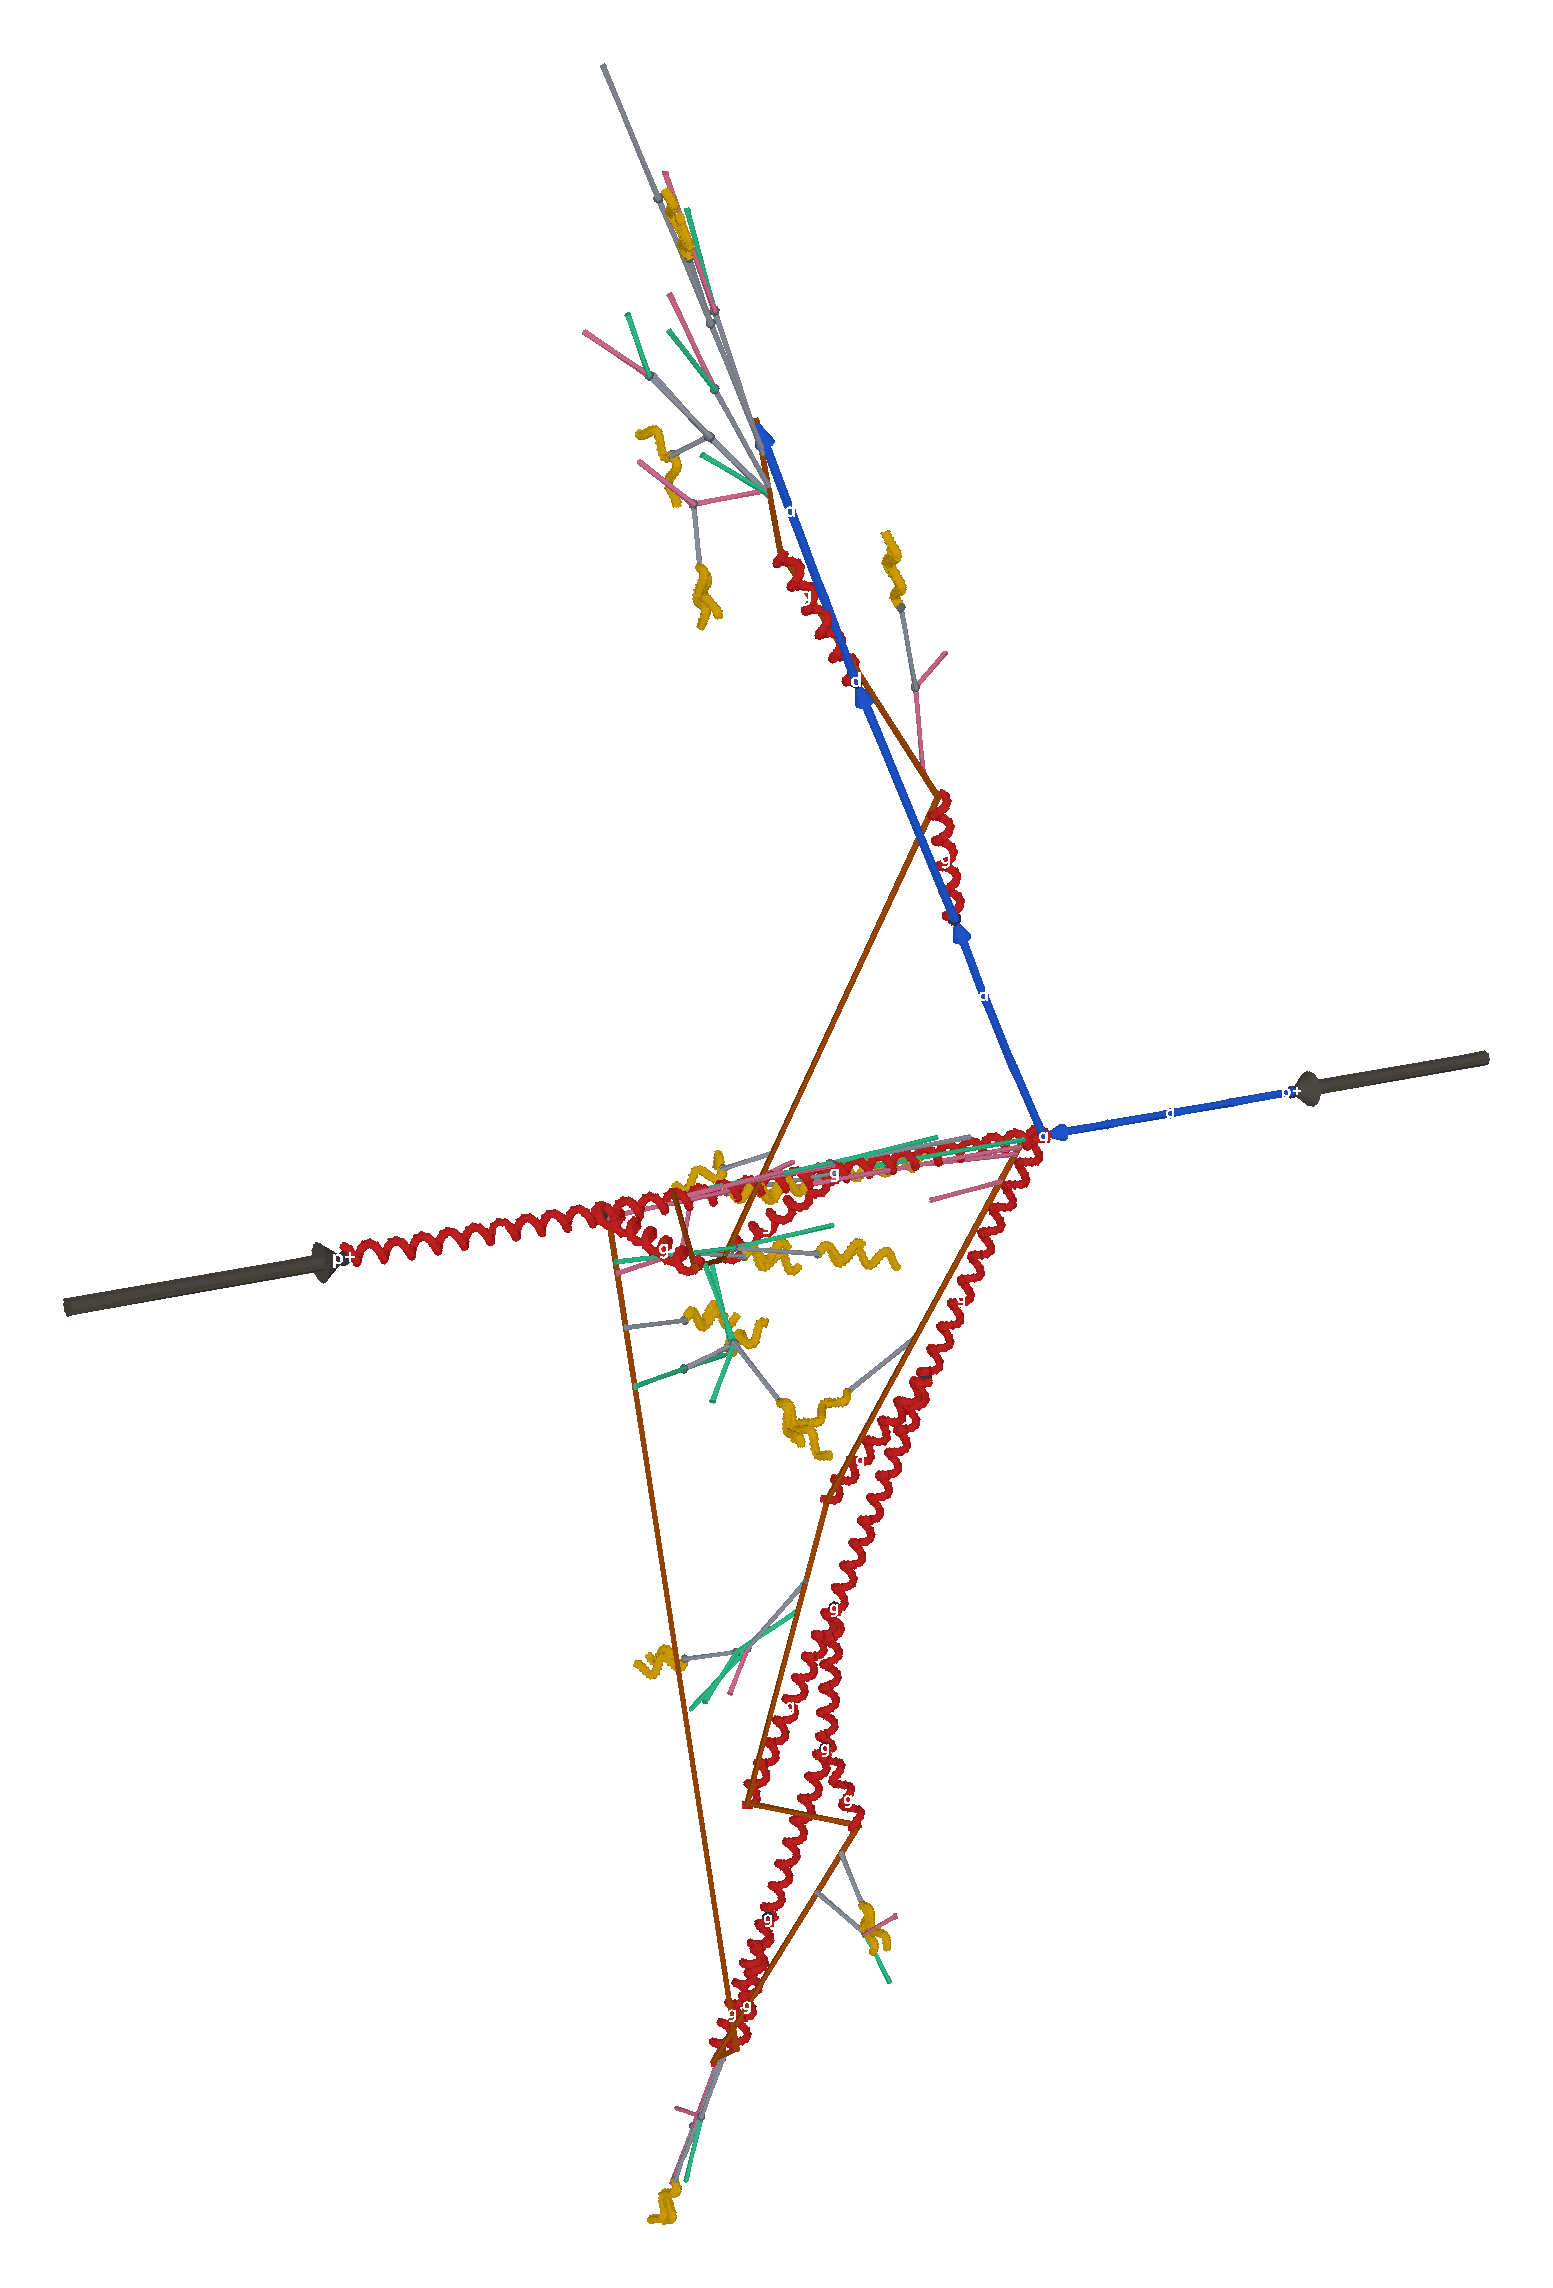
\includegraphics[height=0.66\textheight]{partonShower/qg2qg_hadr.pdf}};
		\node[callout, anchor=east] (shw) at (-2.4,1.3) {Hard-scattered partons highly \textbf{virtual} \(\to\) radiate gluons, \(g \to q\bar{q}\): \textbf{parton shower} (ISR + FSR)};
		\node[callout, anchor=west, visible on=<2->] (soft) at (2.4,-1.2) {Emissions mostly soft or collinear; shower stops at \(\sim 1\)~GeV};
		\node[callout, anchor=west, visible on=<3->] (had) at (2.4,1.3) {\textbf{Hadronization}: non-perturbative, modeled (string, cluster)};
		\node[callout, anchor=east, visible on=<4->] (gen) at (-2.4,-1.2) {Generators: \PYsix, \PYeight, \HWseven};
		% unit square on the shower image
		\begin{scope}[shift={(sh.south west)}, x={($(sh.south east)-(sh.south west)$)}, y={($(sh.north west)-(sh.south west)$)}]
			\draw[pointer, visible on=<1-2>] (shw.east) -- (0.56,0.80);   % outgoing (scattered) quark
			% ISR on the incoming gluon, FSR off the outgoing quark (label style of fig:partonShowerStages)
			\node[font=\scriptsize\sffamily, inner sep=1pt, visible on=<1-2>] (isr) at (0.22,0.33) {ISR};
			\draw[-{Stealth[length=1.6mm]}, thin, black!80, visible on=<1-2>] (isr) -- (0.42,0.47);
			\node[font=\scriptsize\sffamily, inner sep=1pt, visible on=<1-2>] (fsr) at (0.82,0.78) {FSR};
			\draw[-{Stealth[length=1.6mm]}, thin, black!80, visible on=<1-2>] (fsr) -- (0.62,0.72);
			\draw[pointer, visible on=<2>] (soft.west) -- (0.50,0.08);    % soft end of the gluon shower
		\end{scope}
		% unit square on the hadron image
		\begin{scope}[shift={(hd.south west)}, x={($(hd.south east)-(hd.south west)$)}, y={($(hd.north west)-(hd.south west)$)}]
			\draw[pointer, visible on=<3->] (had.west) -- (0.45,0.86);     % hadrons along the quark jet
			\draw[pointer, visible on=<3->] (had.south west) -- (0.43,0.30); % color string
		\end{scope}
	\end{tikzpicture}
	\vfill
	\onslide<4->{%
		\begin{beamercolorbox}[wd=0.85\linewidth, sep=5pt, rounded=true, center]{block body}
			\small\textbf{Jet} = collimated hadron spray that traces its parton's shower
		\end{beamercolorbox}}
\end{frame}

\begin{frame}{Finding jets}
	\begin{columns}[c]
		\begin{column}{0.39\textwidth}
			\begin{itemize}
				\item Jet = algorithm; same on partons, hadrons, detector
				\item<2-> \textbf{anti-\(k_\mathrm{T}\)}: hardest first \(\Rightarrow\) cone-like, radius \(R\)
				\item<3-> IRC safe: insensitive to soft/collinear splits
				\item<4-> Here: \(R = 0.4\), FastJet
			\end{itemize}
		\end{column}
		\begin{column}{0.59\textwidth}
			\centering
			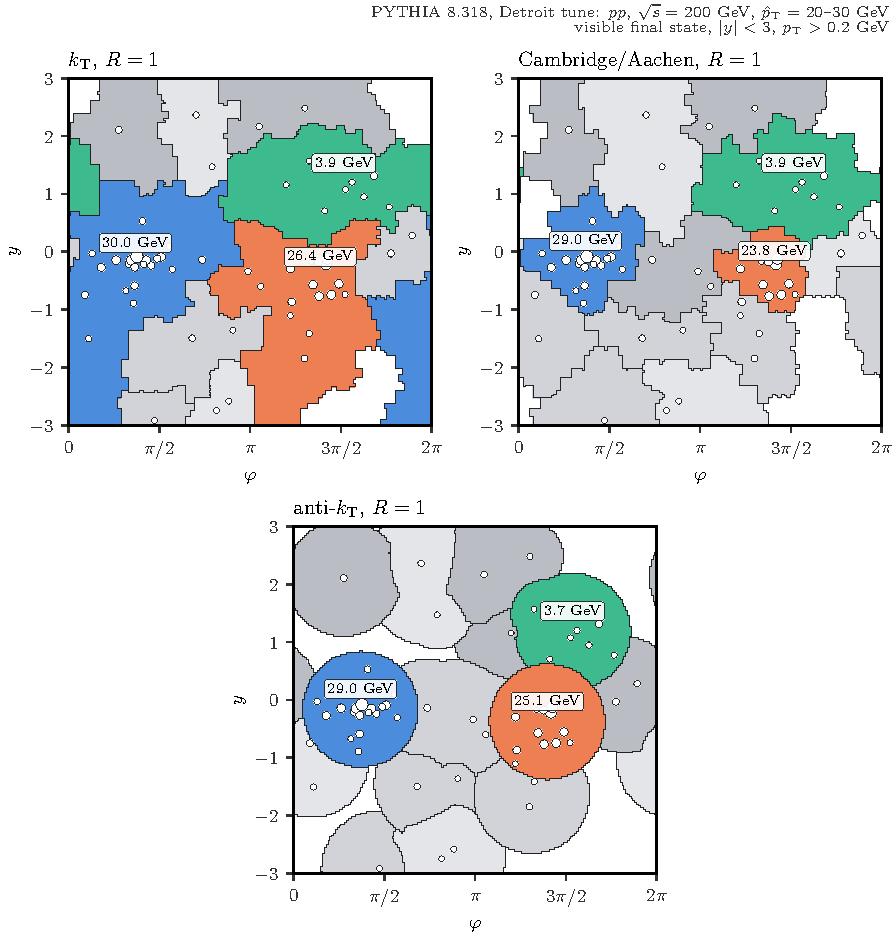
\includegraphics[width=\linewidth,height=0.78\textheight,keepaspectratio]{jet_areas.pdf}
		\end{column}
	\end{columns}
	\refnote{Cacciari, Salam, Soyez, JHEP 04 (2008) 063}
\end{frame}

\begin{frame}{Heavy-ion collisions and the quark-gluon plasma}
	\begin{columns}[c]
		\begin{column}{0.39\textwidth}
			\begin{itemize}
				\item Hot, dense matter \(\to\) \textbf{QGP}; universe \(\mu\)s after Big Bang
				\item<2-> Heavy-ion collisions: pre-equilibrium \(\to\) QGP \(\to\) hadrons \(\to\) freeze-out
				\item<3-> Too short-lived \(\Rightarrow\) self-generated probes
			\end{itemize}
		\end{column}
		\begin{column}{0.59\textwidth}
			\centering
			\only<1>{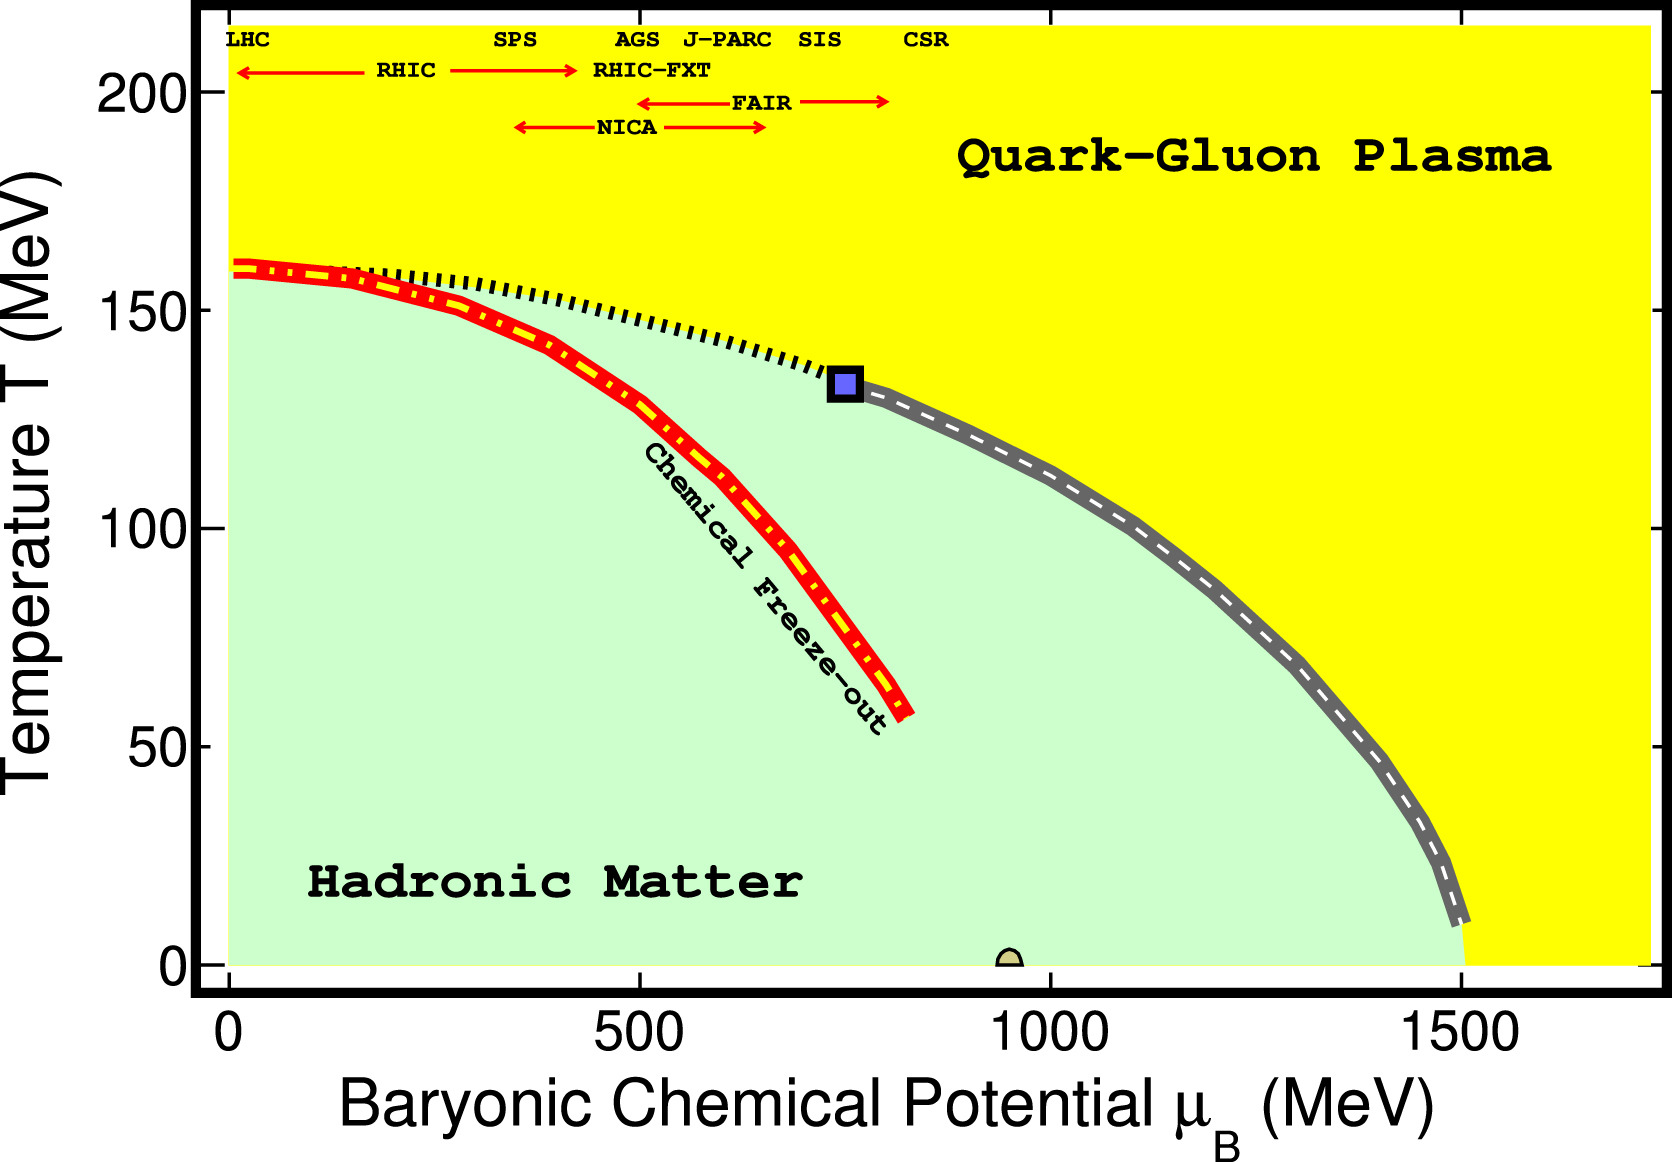
\includegraphics[width=\linewidth,height=0.78\textheight,keepaspectratio]{qcd_phase_diagram.jpg}}%
			\only<2->{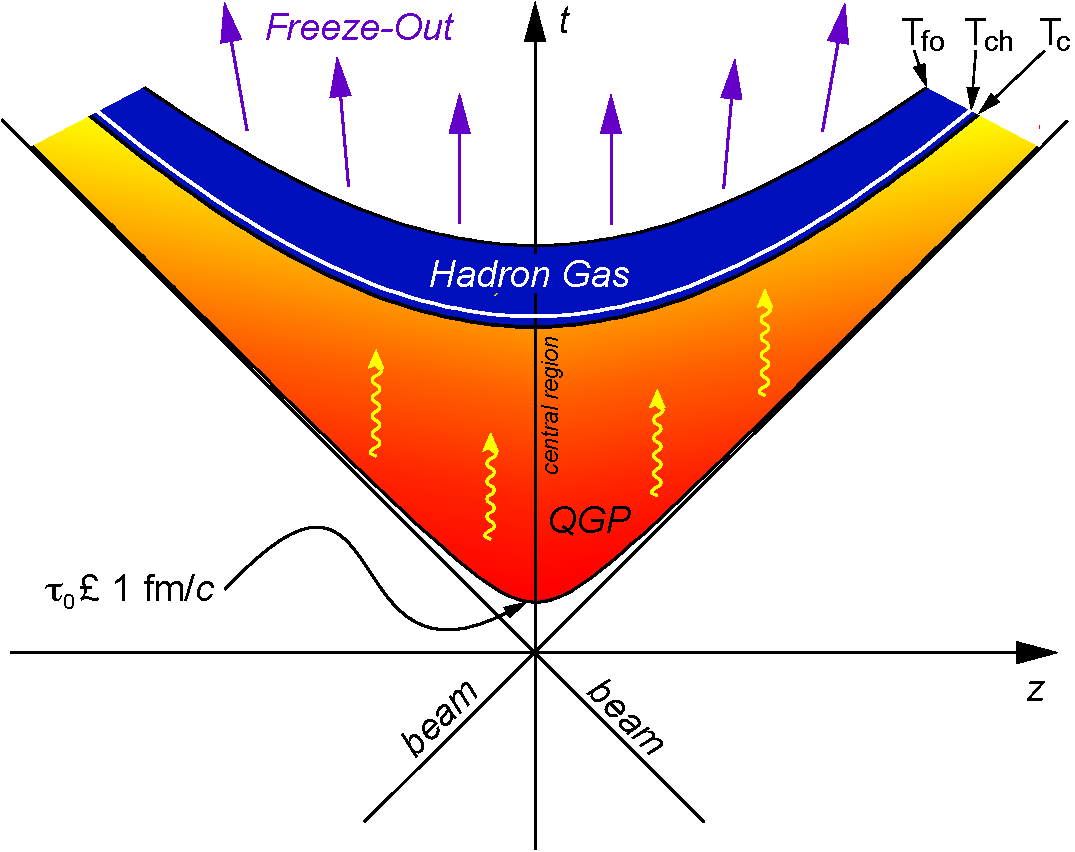
\includegraphics[width=\linewidth,height=0.78\textheight,keepaspectratio]{LightCone1_color-crop}}
		\end{column}
	\end{columns}
\end{frame}

\begin{frame}{Centrality}
	\begin{columns}[c]
		\begin{column}{0.39\textwidth}
			\small
			\begin{itemize}
				\item Impact parameter \(b\): not measurable
				\item<2-> Proxy: charged multiplicity \(N_\mathrm{ch}\) \(\Rightarrow\) \textbf{centrality} classes
				\item<3-> Glauber MC: \(b \to N_\mathrm{part}, N_\mathrm{coll}\) + 2-component model:
				      {\footnotesize\[\frac{dN_\mathrm{ch}}{d\eta} = n_{pp}\Big[x N_\mathrm{coll} + (1-x)\tfrac{N_\mathrm{part}}{2}\Big]\]}
				\item<4-> 0--5\% = top 5\% of \(N_\mathrm{ch}\); \(\langle N_\mathrm{part} \rangle\), \(\langle N_\mathrm{coll} \rangle\) per class
			\end{itemize}
		\end{column}
		\begin{column}{0.59\textwidth}
			\centering
			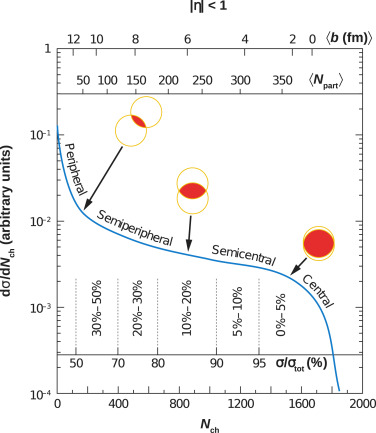
\includegraphics[width=\linewidth,height=0.78\textheight,keepaspectratio]{centrality_refmult.jpg}
		\end{column}
	\end{columns}
	\refnote{Miller et al., Ann.\ Rev.\ Nucl.\ Part.\ Sci.\ 57 (2007) 205}
\end{frame}

\begin{frame}{Collective flow}
	\begin{columns}[c]
		\begin{column}{0.39\textwidth}
			\begin{itemize}
				\item Non-central: almond-shaped overlap
				\item<2-> Pressure gradients \(\to\) momentum anisotropy \(v_2\) w.r.t.\ \textbf{event plane}
				\item<3-> Near-ideal hydro \(\Rightarrow\) strongly coupled liquid
				\item<4-> In- vs out-of-plane jets: \alert{different path lengths}
			\end{itemize}
		\end{column}
		\begin{column}{0.59\textwidth}
			\centering
			\begin{tikzpicture}
				\node[anchor=south west, inner sep=0] (ini) at (0,0) {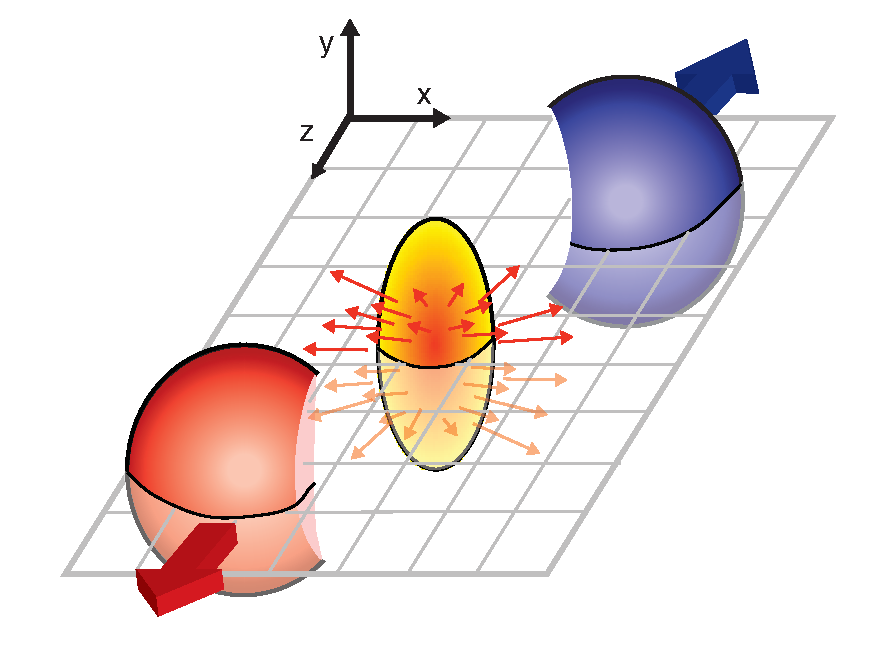
\includegraphics[width=0.48\linewidth]{flow_elliptic_init_v4.pdf}};
				% the grid is the x-z plane: beam (z) and impact parameter (x)
				\begin{scope}[x={(ini.south east)}, y={(ini.north west)}]
					\node[font=\scriptsize, anchor=north, text=PrimaryColor] (rp) at (0.62,-0.02) {reaction plane \(\Psi_\mathrm{RP}\)};
					\draw[-{Stealth[length=1.6mm]}, PrimaryColor, thin] (rp.north) -- (0.58,0.19);
				\end{scope}
			\end{tikzpicture}\hfill
			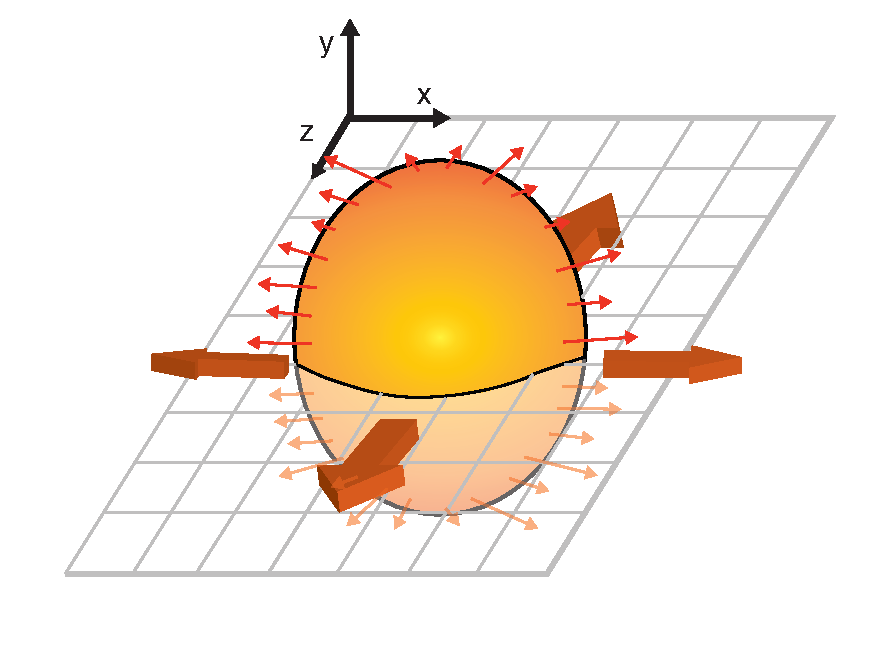
\includegraphics[width=0.48\linewidth]{flow_elliptic_expd_xyz_v2.pdf}\\[1mm]
			\begin{overlayarea}{\linewidth}{0.4\textheight}
				\centering
				% click 2: Psi_RP is not measured; the 2nd-order event plane approximates it (App. EP reconstruction)
				\only<2>{%
					\begin{tikzpicture}[scale=1.0, >={Stealth[length=1.6mm]}]
						\draw[dashed, gray] (-1.6,0) -- (1.6,0) node[below right, font=\scriptsize, text=black!70, inner sep=1pt] {\(\Psi_\mathrm{RP}\)};
						% particles: more and harder along the reaction plane (elliptic flow)
						\foreach \p in {0,22,45,67,90,112,135,157,180,202,225,247,270,292,315,337} {
								\pgfmathsetmacro{\r}{0.7+0.55*cos(2*\p)}
								\draw[->, thin, black!70] (0,0) -- (\p+8:\r);
							}
						\draw[thick, PrimaryColor] (200:1.6) -- (20:1.6) node[above right, font=\scriptsize, text=PrimaryColor, inner sep=1pt] {\(\Psi_{2,\mathrm{EP}}\)};
						\draw[PrimaryColor] (0:1.45) arc[start angle=0, end angle=20, radius=1.45];
					\end{tikzpicture}\hspace{1mm}%
					\parbox[c]{0.5\linewidth}{\raggedright\footnotesize
						\(\Psi_\mathrm{RP}\) not measurable \(\to\) event plane from tracks:\\[1mm]
						\(\Psi_{2,\mathrm{EP}} = \tfrac{1}{2}\arctan(Q_{y,2}/Q_{x,2})\)\\[1mm]
						\(\mathbf{Q}_2 = \sum_\mathrm{tracks} p_\mathrm{T} (\cos 2\phi, \sin 2\phi)\)\\[1mm]
						\(R_2 = \langle \cos 2(\Psi_{2,\mathrm{EP}} - \Psi_\mathrm{RP}) \rangle\)}}%
				\only<3->{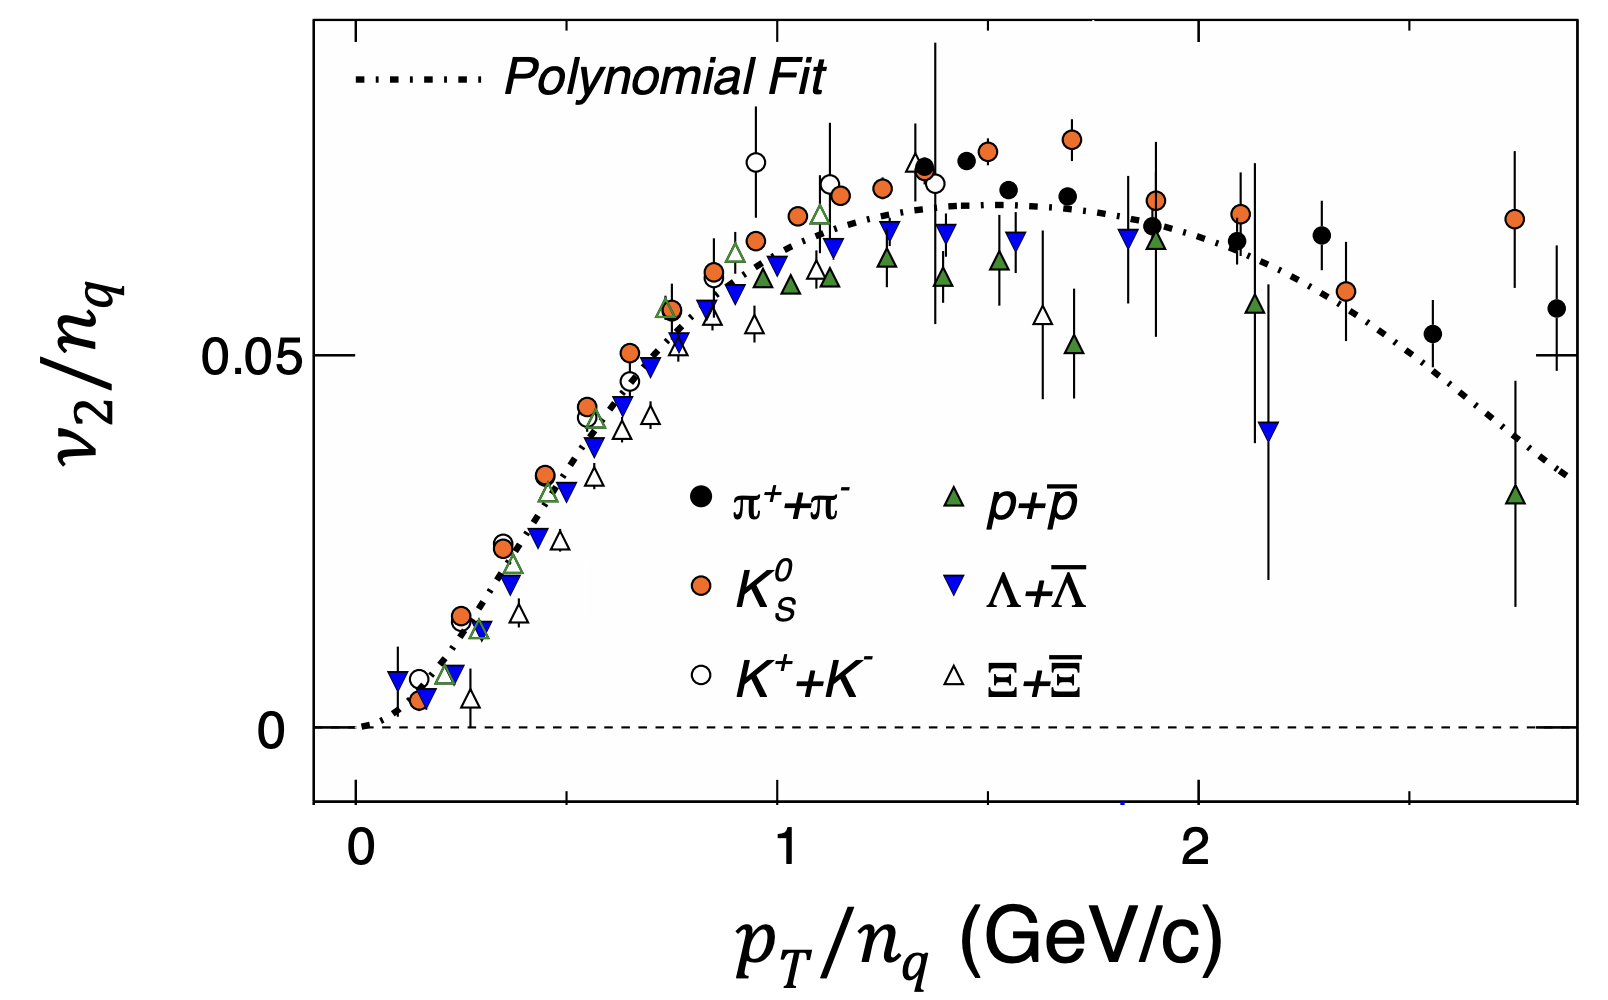
\includegraphics[width=0.6\linewidth]{Gen1_IdentifiedParticle_v2.png}}
			\end{overlayarea}
		\end{column}
	\end{columns}
\end{frame}

\begin{frame}{Jet quenching}
	\begin{columns}[c]
		\begin{column}{0.39\textwidth}
			% fixed, top-aligned box so the first bullet never moves between clicks
			\parbox[c][0.83\textheight][t]{\linewidth}{%
			\begin{itemize}
				\item Partons lose energy in QGP
			\end{itemize}
			% di-hadron correlation cartoon (click 3), transverse plane
			\only<3>{%
			\centering
			\begin{tikzpicture}[scale=1.1,
				trig/.style={-{Stealth[length=2.5mm]}, line width=1.6pt, PrimaryColor},
				assoc/.style={-{Stealth[length=1.8mm]}, thick, black!70},
				lbl/.style={font=\scriptsize, align=center, inner sep=1pt}]
				% QGP in the transverse plane; hard scattering near its surface
				\shade[inner color=orange!70, outer color=orange!15] (0,0) ellipse [x radius=1.25, y radius=1.6];
				\node[lbl, text=orange!40!black, font=\scriptsize\bfseries] at (-0.1,1.2) {QGP};
				\coordinate (hs) at (0.85,0.25);
				% trigger: short path, escapes with its near-side partners
				\draw[trig] (hs) -- (2.3,0.65) node[lbl, right, text=PrimaryColor] {trigger:\\[-1pt]short path};
				% associated hadrons at the angles of the earlier cartoon, relative to the trigger (15.5 deg):
				% near side -15, +15, +50 deg; away side +170, +185, +205 deg
				\foreach \a/\l in {0.5/1.3, 30.5/1.15, 65.5/1.25} \draw[assoc] (hs) -- ++(\a:\l);
				\foreach \a/\l in {185.5/1.3, 200.5/1.5, 220.5/1.1} \draw[assoc, black!40] (hs) -- ++(\a:\l);
				\draw[thin] ($(hs)+(15.5:0.6)$) arc[start angle=15.5, end angle=65.5, radius=0.6];
				\node[lbl] at ($(hs)+(40:0.85)$) {\(\Delta\phi\)};
				% away side: long path through the QGP, absorbed
				\draw[line width=1.6pt, PrimaryColor!70, densely dashed] (hs) -- (-0.85,-0.15);
				\draw[line width=1.6pt, PrimaryColor!25, densely dotted, -{Stealth[length=2mm]}] (-0.85,-0.15) -- (-1.15,-0.22);
				\node[lbl, text=red!60!black, font=\large] at (-0.9,-0.16) {\(\times\)};
				\node[lbl, anchor=north] at (-0.75,-0.35) {away side:\\[-1pt]long path,\\[-1pt]absorbed};
				\fill (hs) circle (1.6pt);
			\end{tikzpicture}\\[1mm]
			{\small \(\Delta\phi = \phi_\mathrm{assoc} - \phi_\mathrm{trig}\): \(\displaystyle \frac{1}{N_\mathrm{trig}} \frac{dN_\mathrm{pair}}{d\Delta\phi}\)}}%
			% R_AA / R_CP definitions take this space on clicks 4-5
			\only<4->{%
				\begin{itemize}
					\item Heavy-ion vs scaled \(p+p\):
					      \[R_\mathrm{AA} = \frac{dN_\mathrm{AA}/dp_\mathrm{T}}{\langle T_\mathrm{AA} \rangle\, d\sigma_{pp}/dp_\mathrm{T}}\]
					\item<5-> Central vs scaled peripheral:
					      \[R_\mathrm{CP} = \frac{dN/dp_\mathrm{T} \,/\, \langle N_\mathrm{coll} \rangle \big|_\mathrm{cent}}{dN/dp_\mathrm{T} \,/\, \langle N_\mathrm{coll} \rangle \big|_\mathrm{peri}}\]
				\end{itemize}}%
			}
		\end{column}
		\begin{column}{0.59\textwidth}
			\centering
			% figure and its takeaway centred together in a fixed-height box
			\parbox[c][0.83\textheight][c]{\linewidth}{\centering
				\only<1-2>{%
					\resizebox{!}{0.62\textheight}{%
						\begin{tikzpicture}
							\useasboundingbox (-4.3,-2.6) rectangle (2.2,3.6); % same frame for both steps
							\only<1>{%
								\drawDiJetInVacuum
								\draw[fill=violet!20, rounded corners, opacity=0.2] (-2.0, 3.5) rectangle (0.6, -2.5) node at (-1.0, 3.) {Medium};
							}%
							\only<2>{\drawDiJetInMedium}%
						\end{tikzpicture}}}%
				\only<3>{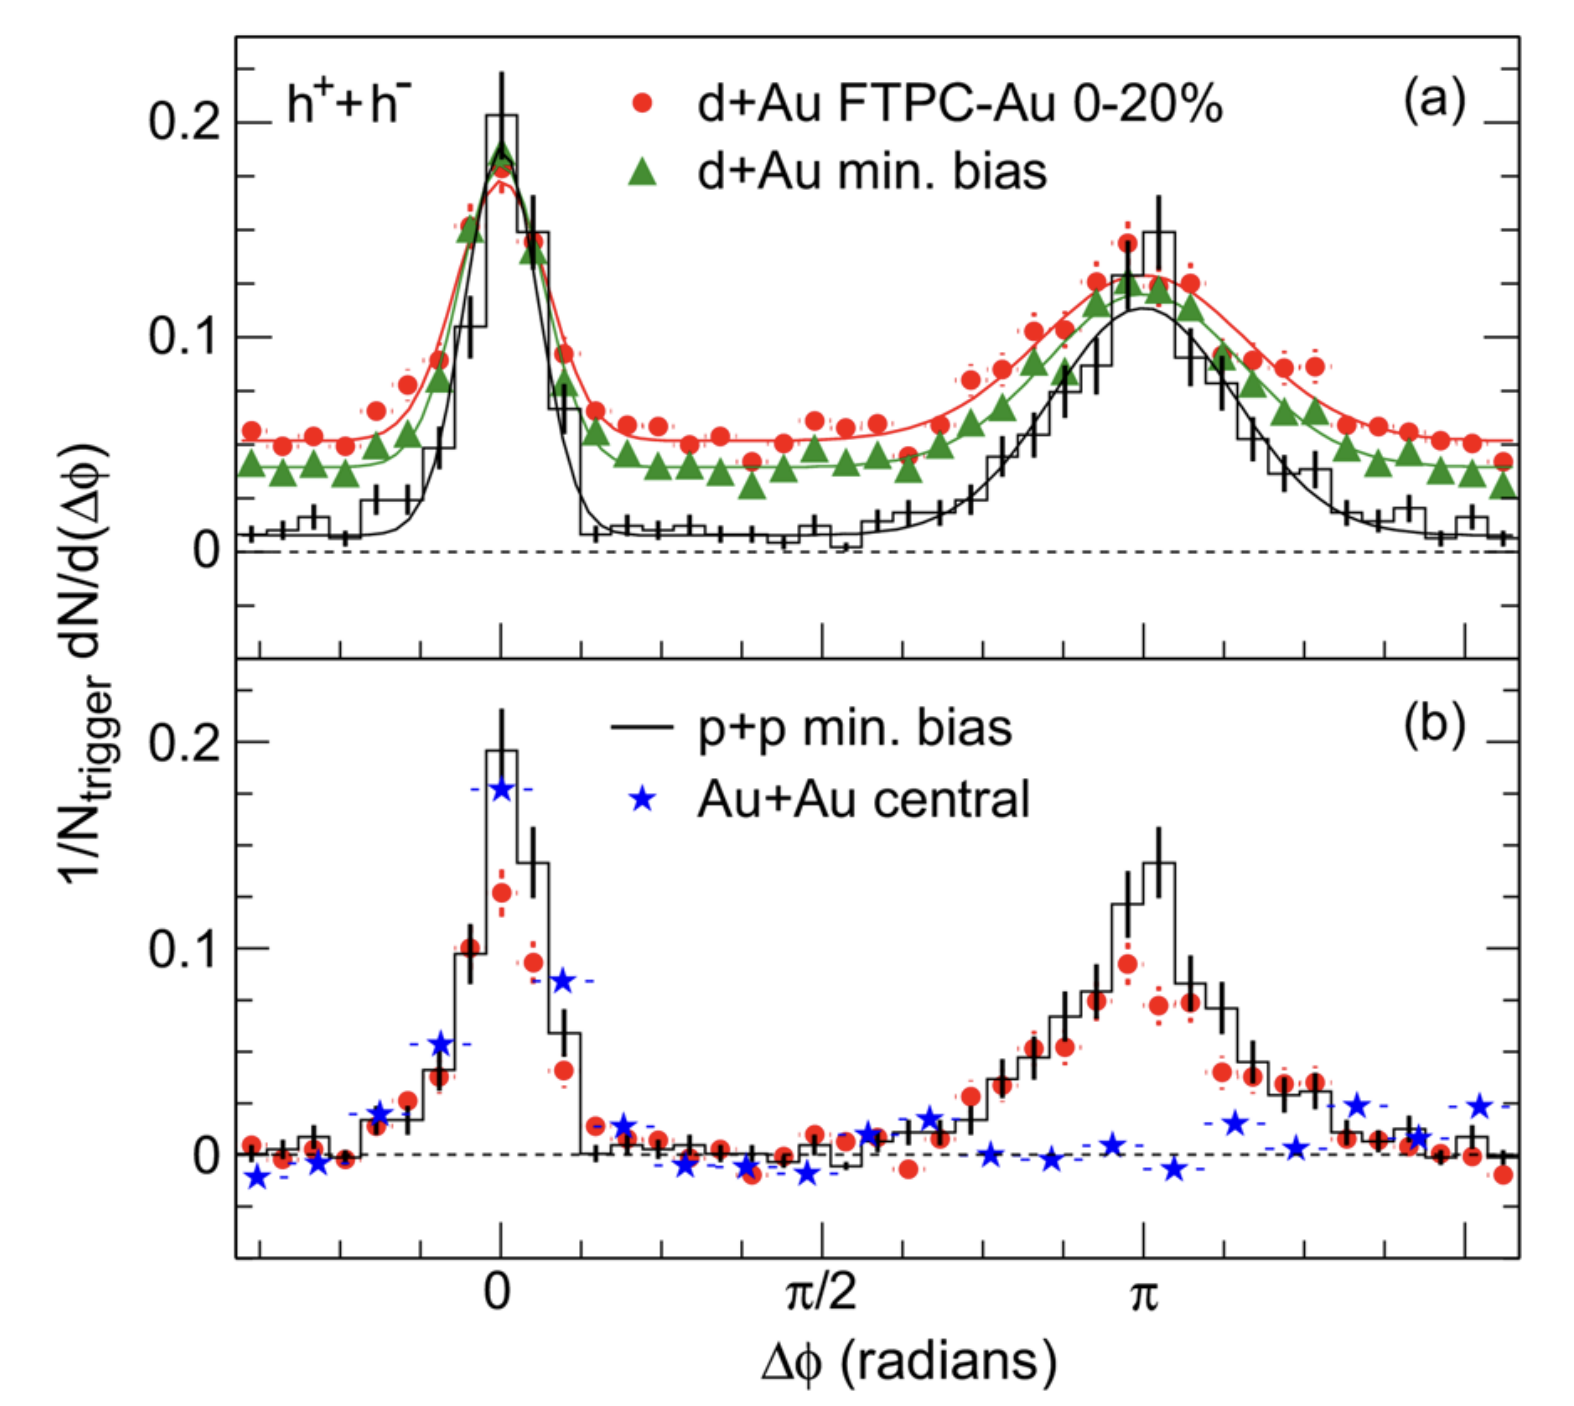
\includegraphics[width=\linewidth,height=0.62\textheight,keepaspectratio]{Gen0_AngularCorrelation_JetQuenching.png}}%
				\only<4>{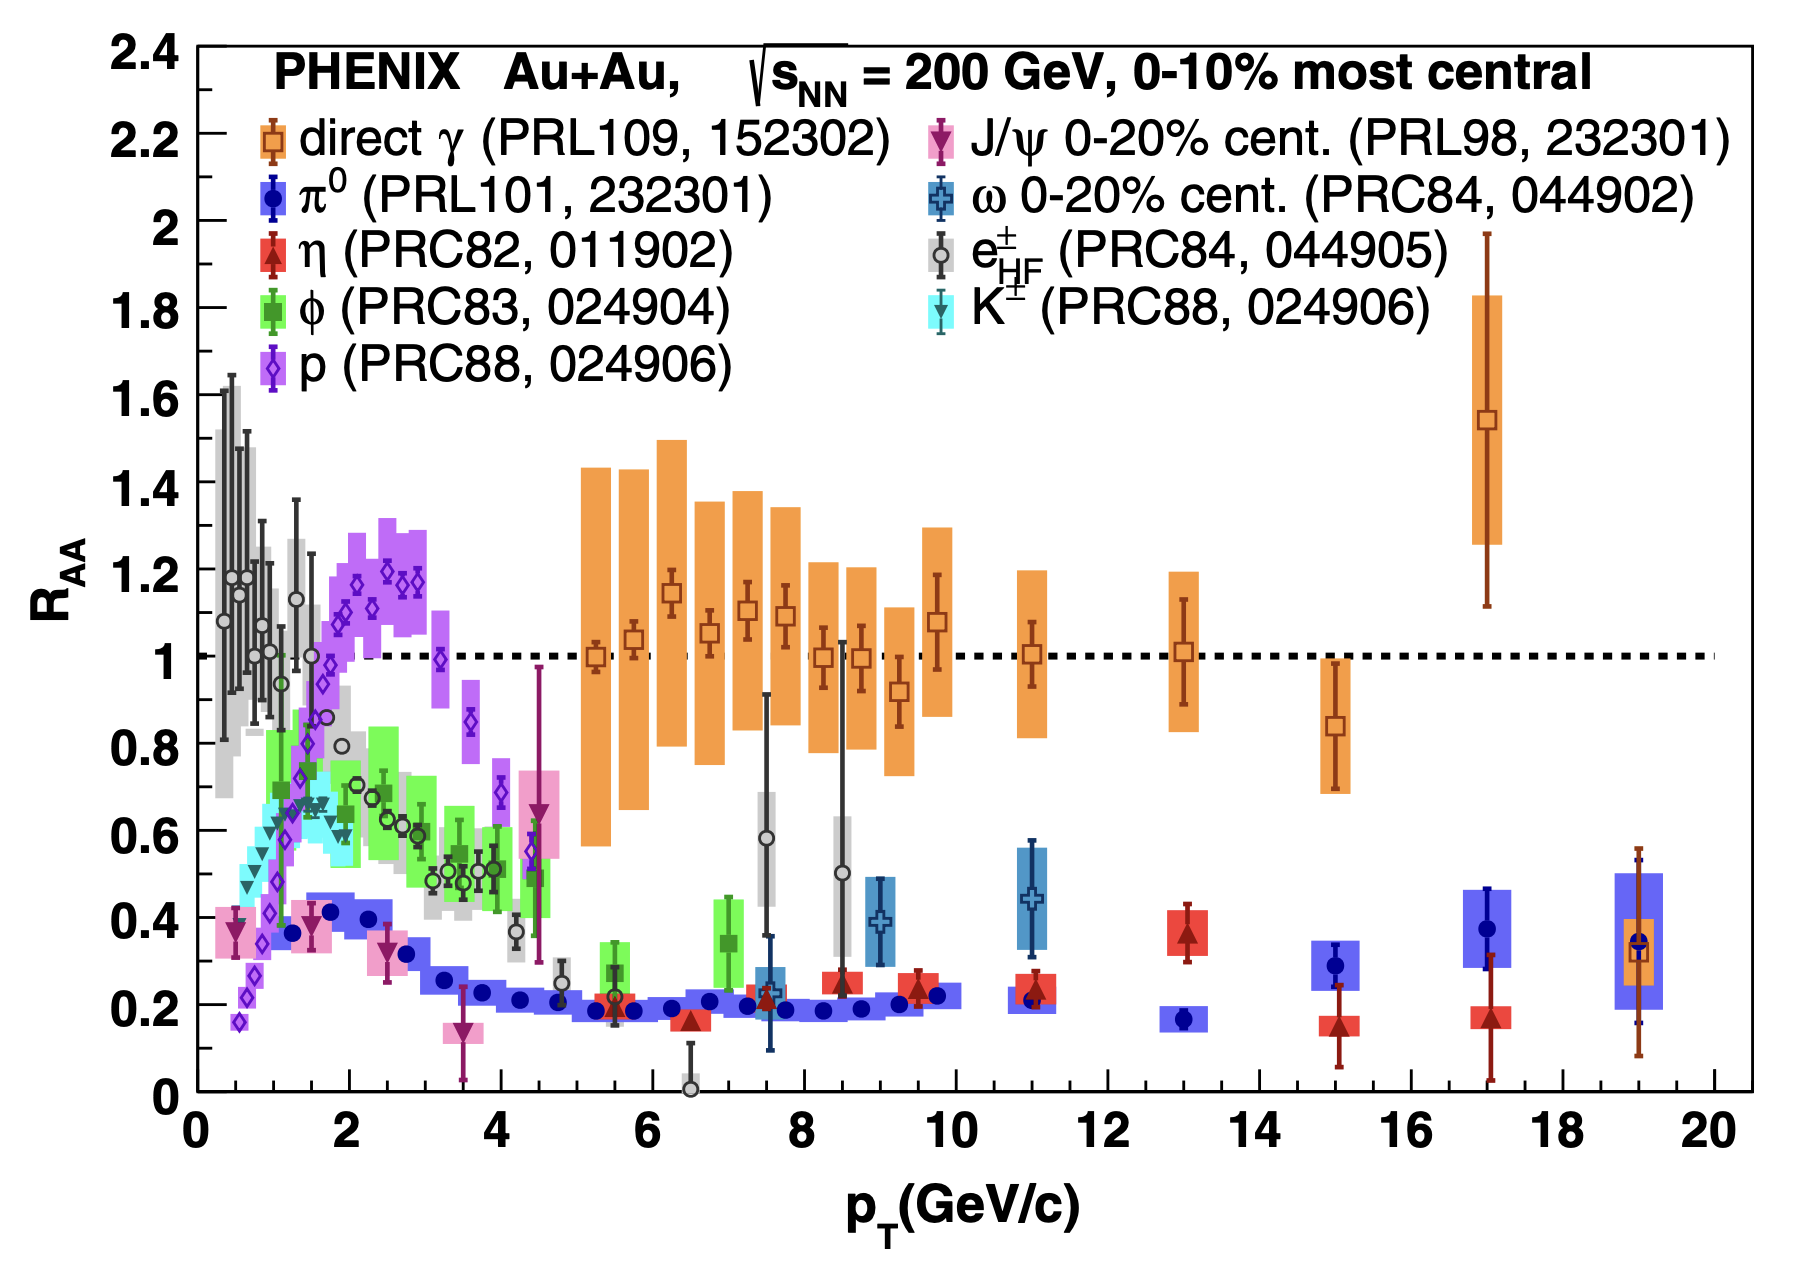
\includegraphics[width=\linewidth,height=0.62\textheight,keepaspectratio]{Gen0_SingleParticle_RAA.png}}%
				\only<5>{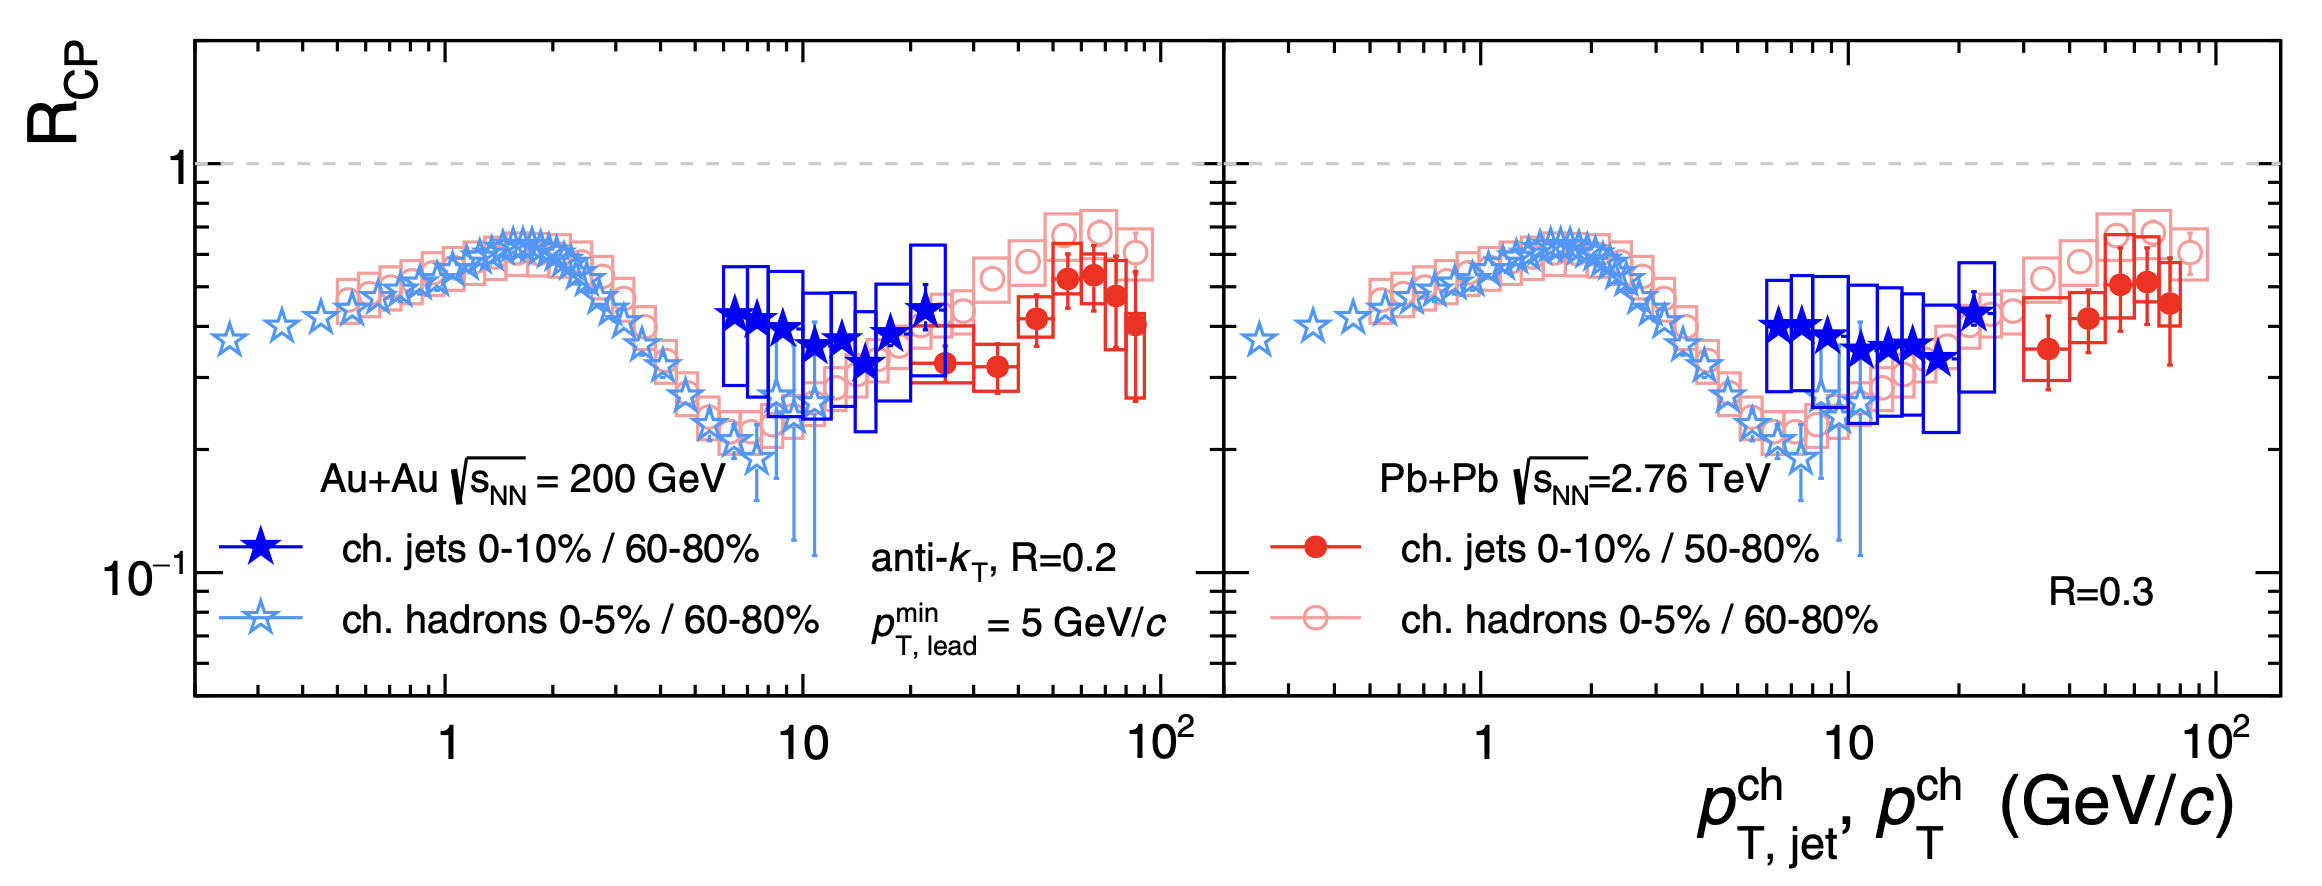
\includegraphics[width=\linewidth,height=0.62\textheight,keepaspectratio]{Gen1_ChargedParticleAndJets_RCP.png}}
				\par\vspace{1mm}
				\only<1-3>{\visible<3>{\begin{beamercolorbox}[wd=\linewidth, sep=4pt, rounded=true, center]{block body}\small Away-side peak vanishes in central Au+Au: recoiling parton quenched\end{beamercolorbox}}}%
			\only<4>{\begin{beamercolorbox}[wd=\linewidth, sep=4pt, rounded=true, center]{block body}\small All hadrons suppressed, \(R_\mathrm{AA} \approx 0.2\)--\(0.6\); direct \(\gamma\) unmodified\end{beamercolorbox}}%
			\only<5>{\begin{beamercolorbox}[wd=\linewidth, sep=4pt, rounded=true, center]{block body}\small Charged jets \(\sim\)60\% suppressed, no \(p_\mathrm{T}\) dependence; same at RHIC and LHC\end{beamercolorbox}}
			}
		\end{column}
	\end{columns}
	\only<3>{\refnote{STAR, PRL 91 (2003) 072304}}%
	\only<4>{\refnote{PHENIX, from Tannenbaum, J.\ Phys.\ Conf.\ Ser.\ 589 (2015) 012019}}%
	\only<5>{\refnote{STAR, PRC 102 (2020) 054913}}
\end{frame}

\begin{frame}{Why look inside jets?}
	\begin{itemize}
		\item \(R_\mathrm{AA}\), \(R_\mathrm{CP}\) \emph{count} jets --- blind to inside
		\item<2-> Medium moves momentum to \textbf{larger angles, lower \(p_\mathrm{T}\)}
		\item<3-> QGP resolves splittings only above some \textbf{angle} (coherence)
		\item<4-> Yields average over \textbf{path length}
	\end{itemize}
	\vspace{3mm}
	\onslide<5->{
		\begin{block}{This thesis}
			\begin{itemize}
				\item Path length: jet-hadron vs event plane (Au+Au)
				\item Energy vs angle: angularities (Au+Au, \(p+p\))
			\end{itemize}
		\end{block}}
	\refnote{Cao, Wang, Rept.\ Prog.\ Phys.\ 84 (2021) 024301; Casalderrey-Solana et al., PLB 725 (2013) 357; Brewer, Milhano, Thaler, PRL 122 (2019) 222301}
\end{frame}

%======================================================================
\section{RHIC and STAR}

\begin{frame}{The Relativistic Heavy Ion Collider}
	\begin{columns}[c]
		\begin{column}{0.59\textwidth}
			\centering
			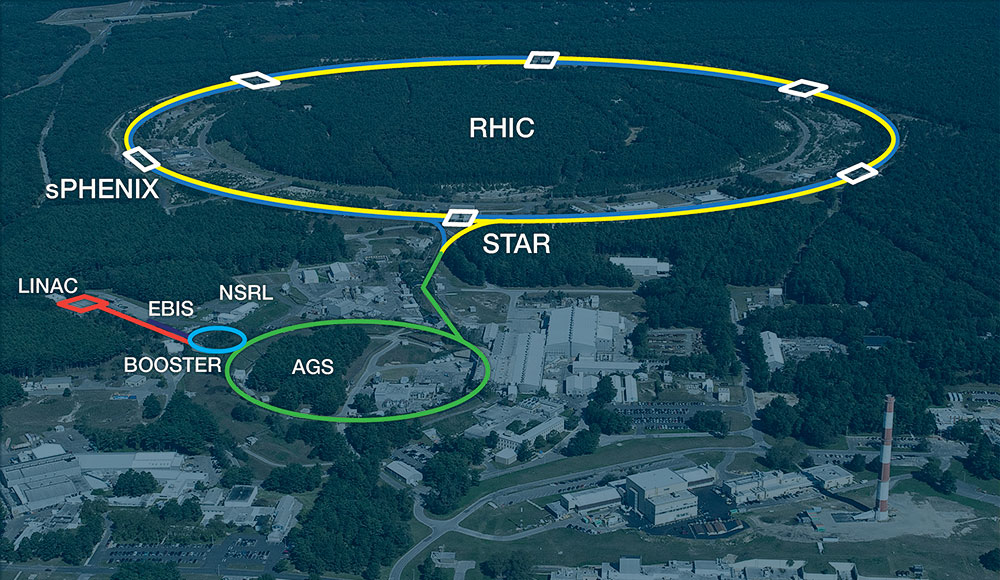
\includegraphics[width=\linewidth]{rhic-aerial-hr.jpg}
		\end{column}
		\begin{column}{0.39\textwidth}
			\begin{itemize}
				\item Operated 2000--2026: dedicated heavy-ion + polarized \(p\) collider
				\item \(\sim\)300 trillion collisions, \(\sim\)450 PB
				\item Last beam: O+O, 6 Feb 2026
				\item Here: Au+Au 2014, \(p+p\) 2012, 200~GeV
			\end{itemize}
		\end{column}
	\end{columns}
\end{frame}

\begin{frame}{The STAR detector}
	\centering
	\begin{tikzpicture}[
		blurb/.style={draw=PrimaryColor, fill=white, rounded corners=3pt, line width=0.8pt,
				text width=2.8cm, align=left, inner sep=4pt, font=\scriptsize, execute at begin node={\hyphenpenalty=10000\exhyphenpenalty=10000}},
		pointer/.style={-{Stealth[length=2mm]}, PrimaryColor, line width=0.8pt}]
		\node[anchor=south west, inner sep=0] (star) at (0,0) {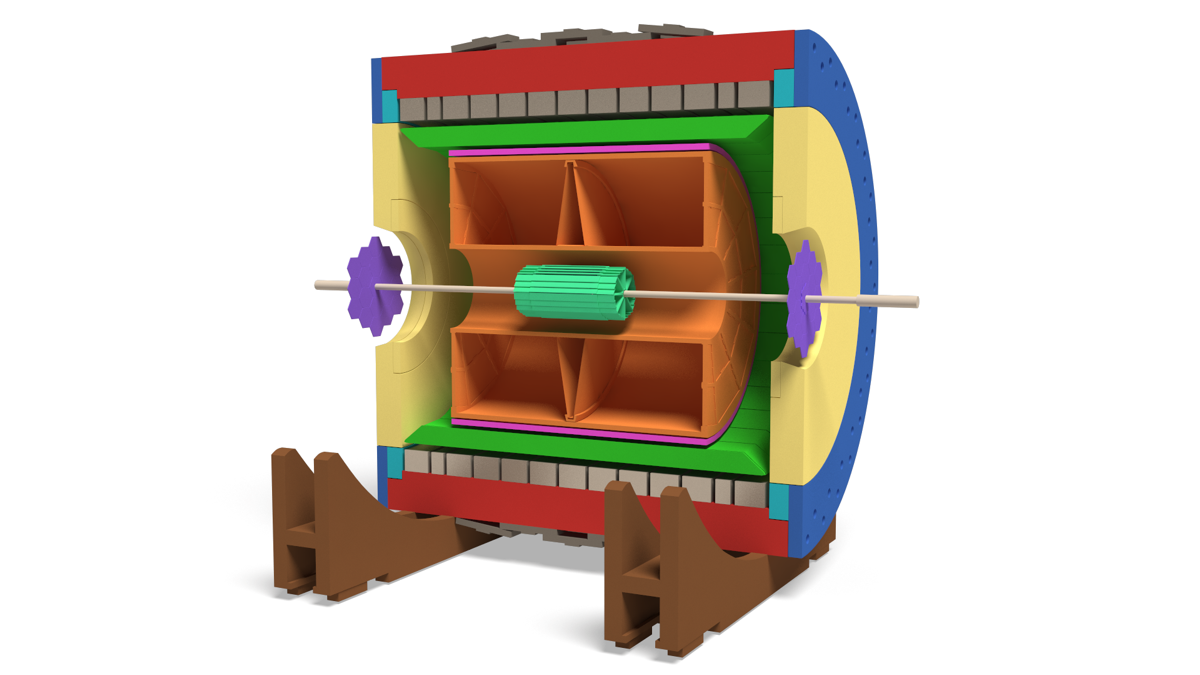
\includegraphics[height=0.58\textheight]{STAR.png}};
		% unit square on the image (1200 x 675 px); arrow targets as in fig:STARDetector
		\begin{scope}[x={(star.south east)}, y={(star.north west)}]
			\node[blurb, anchor=north] (tpc) at (-0.09,-0.04) {\textbf{TPC}: tracks + d\(E\)/d\(x\); \(|\eta| < 1\), full \(\phi\); 0.2--30~GeV/\(c\)};
			\node[blurb, anchor=north] (bemc) at (0.30,-0.04) {\textbf{BEMC}: \(0.05 \times 0.05\) towers; neutral energy; HT trigger};
			\node[blurb, anchor=north] (bbc) at (0.69,-0.04) {\textbf{BBC} (3.7~m): \(3.4 < |\eta| < 5\); \(p+p\) MB trigger, rel.\ luminosity};
			\node[blurb, anchor=north] (fwd) at (1.08,-0.04) {\textbf{VPD} (5.7~m): \(v_z\), start time\\\textbf{ZDC} (18~m): neutrons; MB, luminosity};
			\draw[pointer] (tpc.north) -- (0.43,0.70);
			\draw[pointer] (bemc.north) -- (0.54,0.32);
			\draw[pointer] (bbc.north) -- (0.665,0.52);
			\draw[pointer, dashed] (fwd.north) -- (0.77,0.555) node[pos=0.55, sloped, above, font=\tiny, text=PrimaryColor] {further along beam};
			\node[anchor=west, font=\scriptsize, text=gray] (mag) at (0.80,0.95) {Solenoid: 0.5~T};
			\draw[-{Stealth[length=1.6mm]}, gray, line width=0.6pt] (mag.west) -- (0.55,0.845);
		\end{scope}
	\end{tikzpicture}\\[1mm]
	{\small \textbf{Jets} = TPC tracks + BEMC towers}
\end{frame}

%======================================================================
\section{Jet-hadron correlations relative to the event plane}

\begin{frame}{Jet-hadron correlations: what we measure}
	\begin{columns}[c]
		\begin{column}{0.39\textwidth}
			\small
			\begin{itemize}
				\item Energy loss vs \textbf{path length}?
				\item<2-> Jet angle to event plane \(\Psi_2\): \textbf{in / mid / out-of-plane}
				\item<3-> Hadrons around jet vs \(\Delta\phi, \Delta\eta\): \textbf{yields}, \textbf{widths}
				\item<4-> 20--50\% Au+Au 200~GeV, HT; hard-core jets (cons.\ \(> 2\)~GeV/\(c\)), 15--20, 20--40~GeV/\(c\)
			\end{itemize}
		\end{column}
		\begin{column}{0.59\textwidth}
			\centering
			\begin{tikzpicture}[scale=0.95, >={Stealth[length=2.2mm]}]
				\def\R{2.6}
				% event-plane bins, Eq. Eq:EPbins, mirrored into all four quadrants
				\begin{scope}[visible on=<2->]
					\foreach \c in {0,180} {
							\fill[red!25]  (0,0) -- (\c-30:\R) arc[start angle=\c-30, end angle=\c+30, radius=\R] -- cycle;
							\fill[gray!12] (0,0) -- (\c+30:\R) arc[start angle=\c+30, end angle=\c+60, radius=\R] -- cycle;
							\fill[gray!12] (0,0) -- (\c-60:\R) arc[start angle=\c-60, end angle=\c-30, radius=\R] -- cycle;
							\fill[blue!20] (0,0) -- (\c+60:\R) arc[start angle=\c+60, end angle=\c+120, radius=\R] -- cycle;
						}
					\node[font=\scriptsize\bfseries, text=red!70!black]  at (-15:2.25) {in};
					\node[font=\scriptsize\bfseries, text=black!70]      at (-45:2.25) {mid};
					\node[font=\scriptsize\bfseries, text=blue!70!black] at (-75:2.25) {out};
				\end{scope}
				% overlap region and event plane
				\fill[orange!60, opacity=0.85] (0,0) ellipse [x radius=0.85, y radius=1.45];
				\node[font=\tiny] at (0,-1.1) {QGP};
				\draw[dashed, thick] (\R+0.2,0) -- (-\R-0.2,0) node[left, font=\scriptsize] {\(\Psi_2\)};
				% trigger jet, recoil and associated hadrons
				\begin{scope}[visible on=<3->]
					\draw[->, line width=1.6pt, PrimaryColor] (0.15,0.05) -- (20:\R) node[above, font=\scriptsize, text=PrimaryColor, inner sep=2pt, align=center] {trigger jet\\near side, \(\Delta\phi \approx 0\)};
					\draw[->, line width=1.6pt, PrimaryColor!60] (-0.15,-0.05) -- (200:\R) node[below, font=\scriptsize, text=PrimaryColor!60, inner sep=2pt, align=center] {recoil\\away side, \(\Delta\phi \approx \pi\)};
					\foreach \a/\l in {14/1.5, 27/1.8, 190/1.6, 212/1.8} \draw[->, thin] (0,0) -- (\a:\l);
					\draw[->, thin] (0,0) -- (55:1.75);
					\draw[thick] (20:1.15) arc[start angle=20, end angle=55, radius=1.15] node[midway, above right, font=\scriptsize, inner sep=1pt] {\(\Delta\phi\)};
					\draw[PrimaryColor] (0:2.0) arc[start angle=0, end angle=20, radius=2.0];
					\node[font=\scriptsize, anchor=west, text=PrimaryColor, inner sep=1pt] at (7:2.02) {\(\phi_\mathrm{jet} - \Psi_2\)};
				\end{scope}
			\end{tikzpicture}
		\end{column}
	\end{columns}
	\refnote{STAR, PRC 109 (2024) 044909}
\end{frame}

\begin{frame}{Jet-hadron correlation functions}
	\centering
	\begin{overlayarea}{\linewidth}{0.5\textheight}
		\centering
		\only<1>{%
			\begin{tabular}{@{}c@{\hspace{2pt}}c@{\hspace{2pt}}c@{}}
				{\scriptsize same event}                                                                      & {\scriptsize mixed event} & {\scriptsize same / mixed} \\
				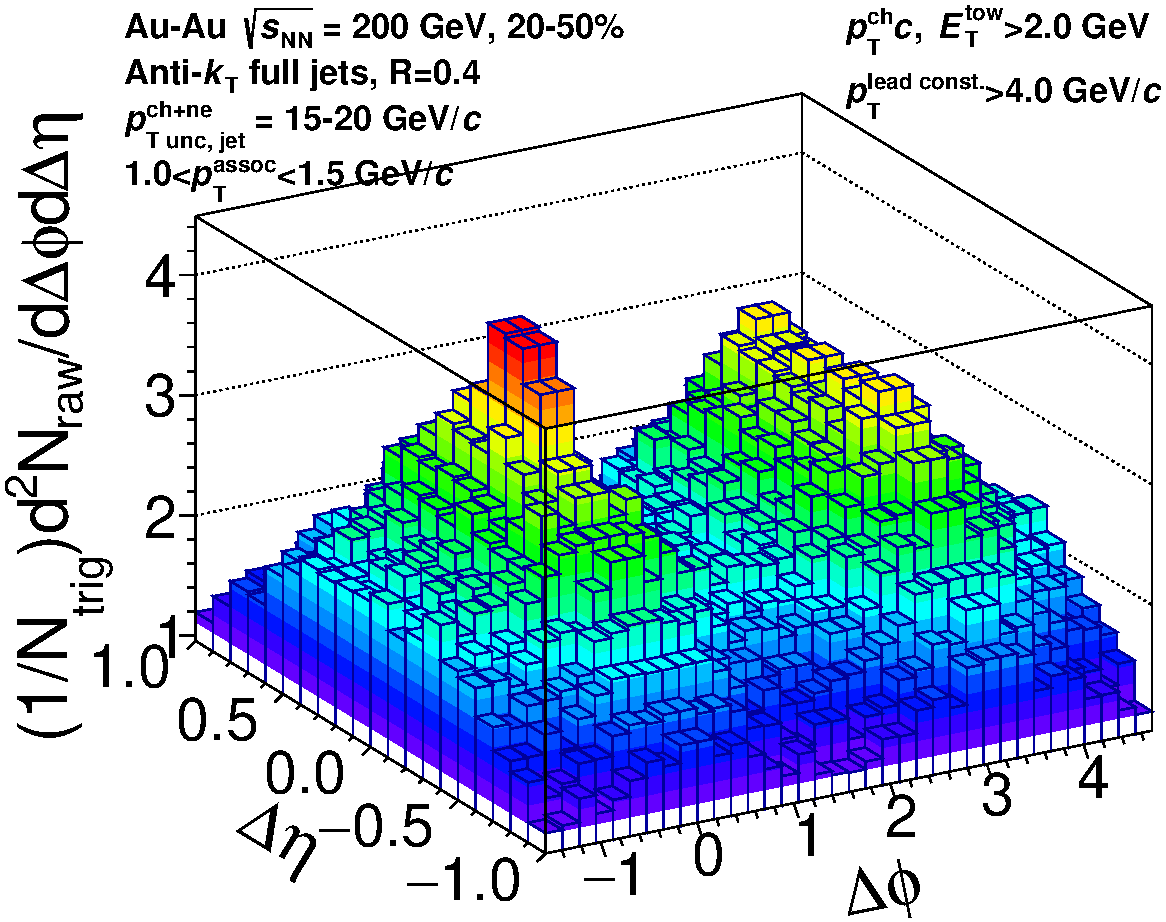
\includegraphics[width=0.325\linewidth]{JHC/J15-20_C20-50_raw2D_sig_in_Ass1.0-1.5_Zcut24.pdf} &
				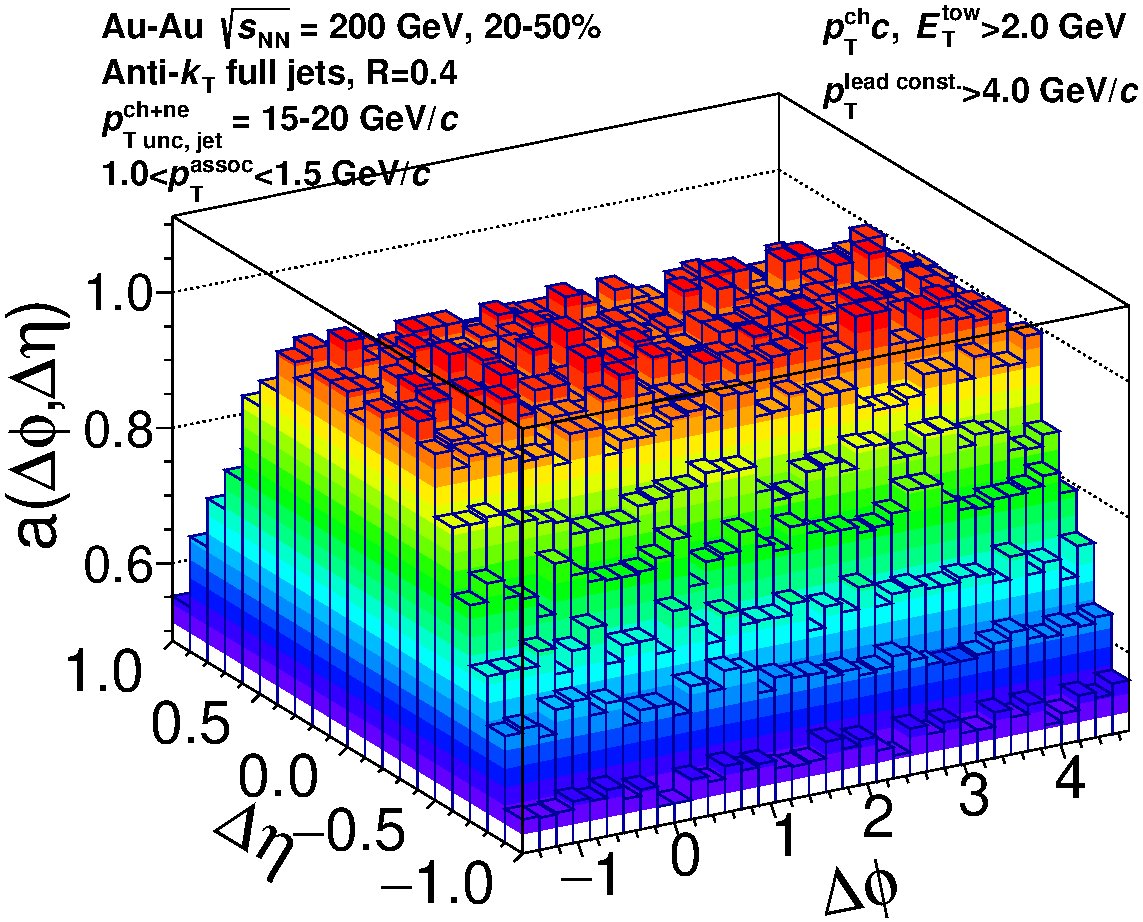
\includegraphics[width=0.325\linewidth]{JHC/J15-20_C20-50_raw2D_mix_in_Ass1.0-1.5_Zcut24.pdf} &
				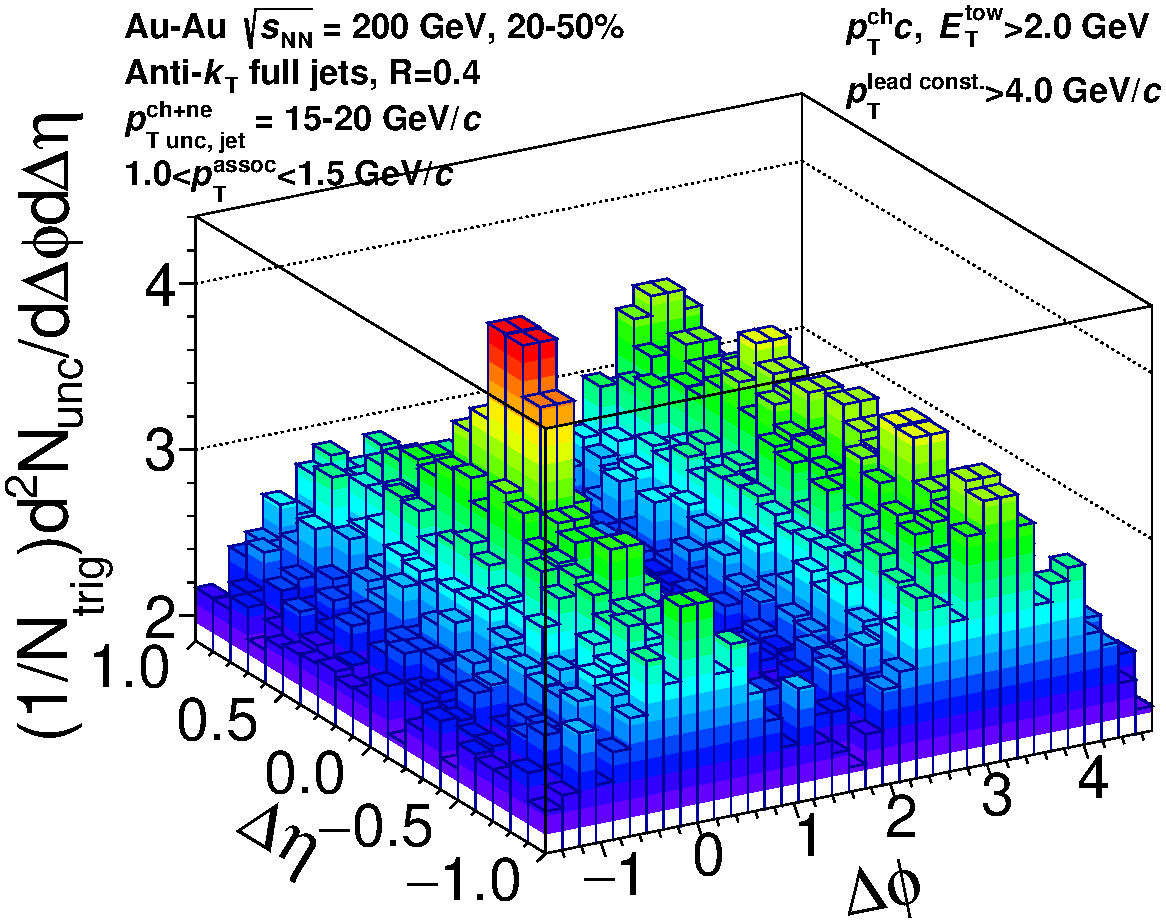
\includegraphics[width=0.325\linewidth]{JHC/J15-20_C20-50_raw2D_ratio_in_Ass1.0-1.5_Zcut24.pdf}
			\end{tabular}}%
		\only<2->{%
			\begin{tikzpicture}
				\node[anchor=south west, inner sep=0] (dphi) at (0,0) {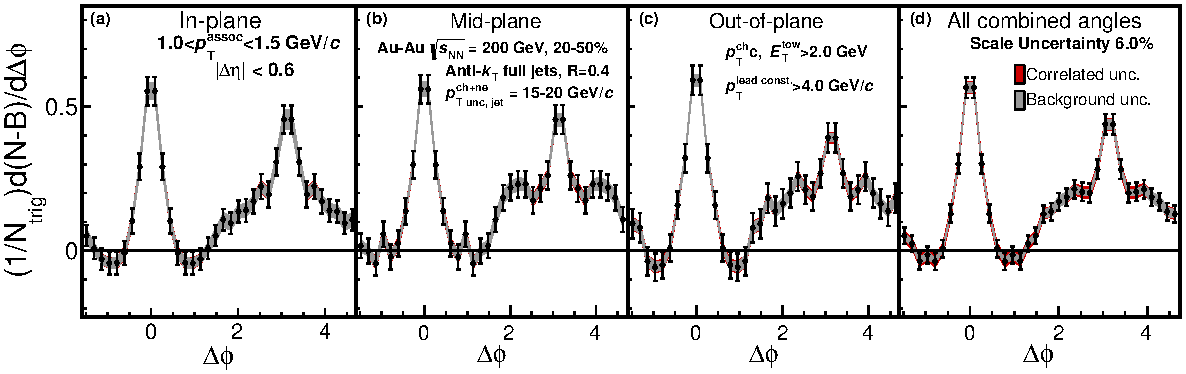
\includegraphics[width=\linewidth,height=0.48\textheight,keepaspectratio]{JHC/dPhiCorrelationsJ15-20_C20-50_1.0-1.5.pdf}};
				% unit square on the image (1186 x 375 px render): panel frames at x = 81/355/627/899/1179 px,
				% plot area y = 5..317 px; each panel spans -pi/2 < dphi < 3pi/2.
				% Per panel: x of dphi = 0 and image widths per radian
				\begin{scope}[x={(dphi.south east)}, y={(dphi.north west)}]
					\foreach \xz/\k in {0.12614/0.036838, 0.35700/0.036433, 0.58600/0.036501, 0.81703/0.037572} {
							\fill[blue!40, opacity=0.3, visible on=<3->]   ({\xz-1.0472*\k},0.155) rectangle ({\xz+1.0472*\k},0.985);  % near side |dphi| < pi/3
							\fill[orange!60, opacity=0.3, visible on=<3->] ({\xz+2.0944*\k},0.155) rectangle ({\xz+4.1888*\k},0.985);  % away side |dphi - pi| < pi/3
						}
				\end{scope}
			\end{tikzpicture}}
	\end{overlayarea}
	\vfill
	\begin{overlayarea}{\linewidth}{0.26\textheight}
		\only<1-2>{%
			\begin{columns}[T]
				\begin{column}{0.49\textwidth}
					\small
					\begin{itemize}
						\item Hadrons around jets in \(\Delta\phi\), \(\Delta\eta\), per trigger jet
						\item Same / mixed event: pair acceptance (trapezoid in \(\Delta\eta\)), \(\varepsilon\) corrected
					\end{itemize}
				\end{column}
				\begin{column}{0.49\textwidth}
					\small
					\begin{itemize}
						\item<2-> Project onto \(\Delta\phi\): in / mid / out-of-plane jets
						\item<2-> Near side \(\Delta\phi \approx 0\), away side \(\Delta\phi \approx \pi\), on flow background
					\end{itemize}
				\end{column}
			\end{columns}}%
		\only<3>{%
		\centering
		\(\displaystyle Y = \frac{1}{N_\mathrm{trig}} \int_{-0.6}^{0.6} d\Delta\eta \int_{a}^{b} d\Delta\phi\, \frac{d^2N_\mathrm{assoc,jet}}{d\Delta\phi\, d\Delta\eta}\)\\[2mm]
		\small{\color{blue!70!black}\textbf{near side}: \([a,b] = [-\pi/3, \pi/3]\)} \qquad {\color{orange!80!black}\textbf{away side}: \([a,b] = [2\pi/3, 4\pi/3]\)}}
	\end{overlayarea}
	\refnote{STAR, PRC 109 (2024) 044909. In-plane 15--20~GeV/\(c\) jets, 1.0--1.5~GeV/\(c\) hadrons, 20--50\%}
\end{frame}

\begin{frame}{Results: yields and their ratios}
	\centering
	\only<1>{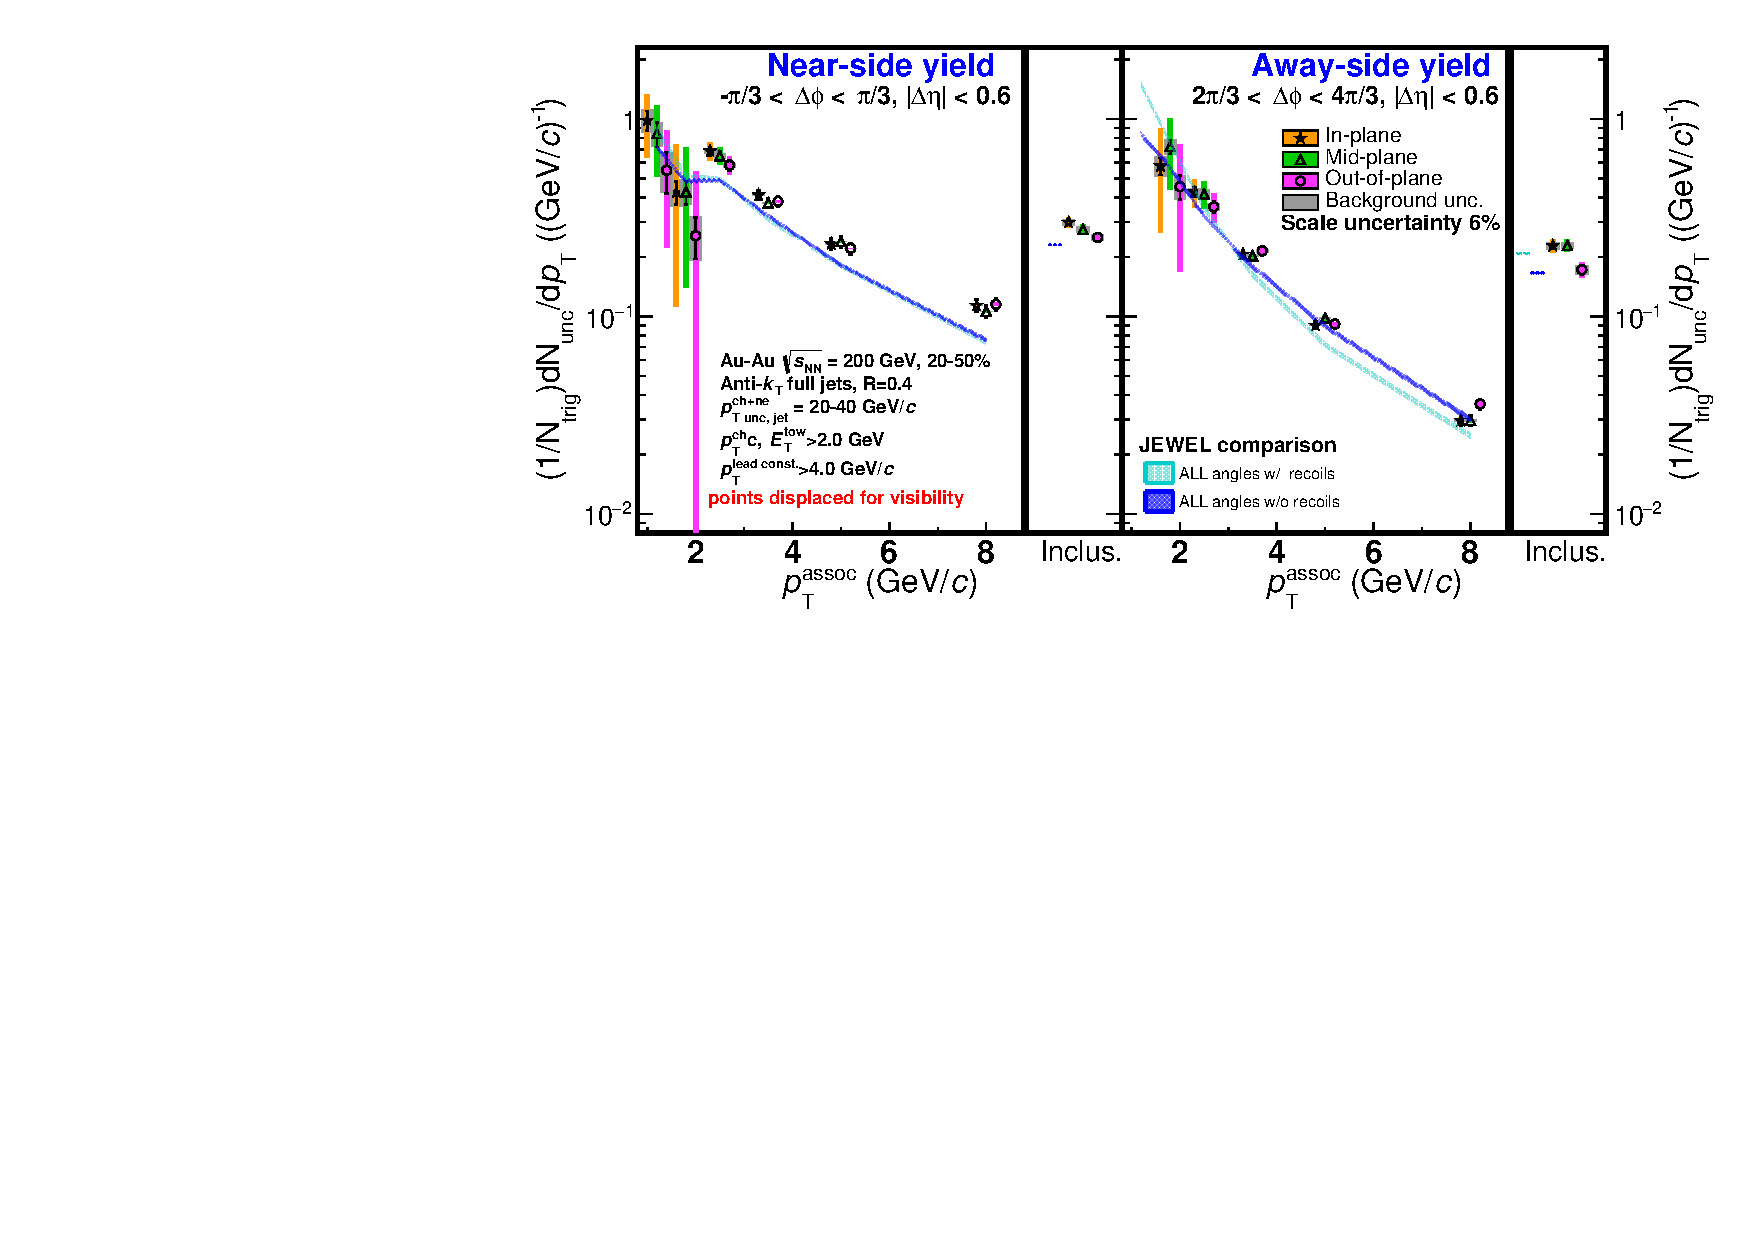
\includegraphics[height=0.6\textheight]{JHC/results/NearAwaySideYield_J20-40_C20-50_wJEScorr_wJEWELerr.pdf}}%
	\only<2->{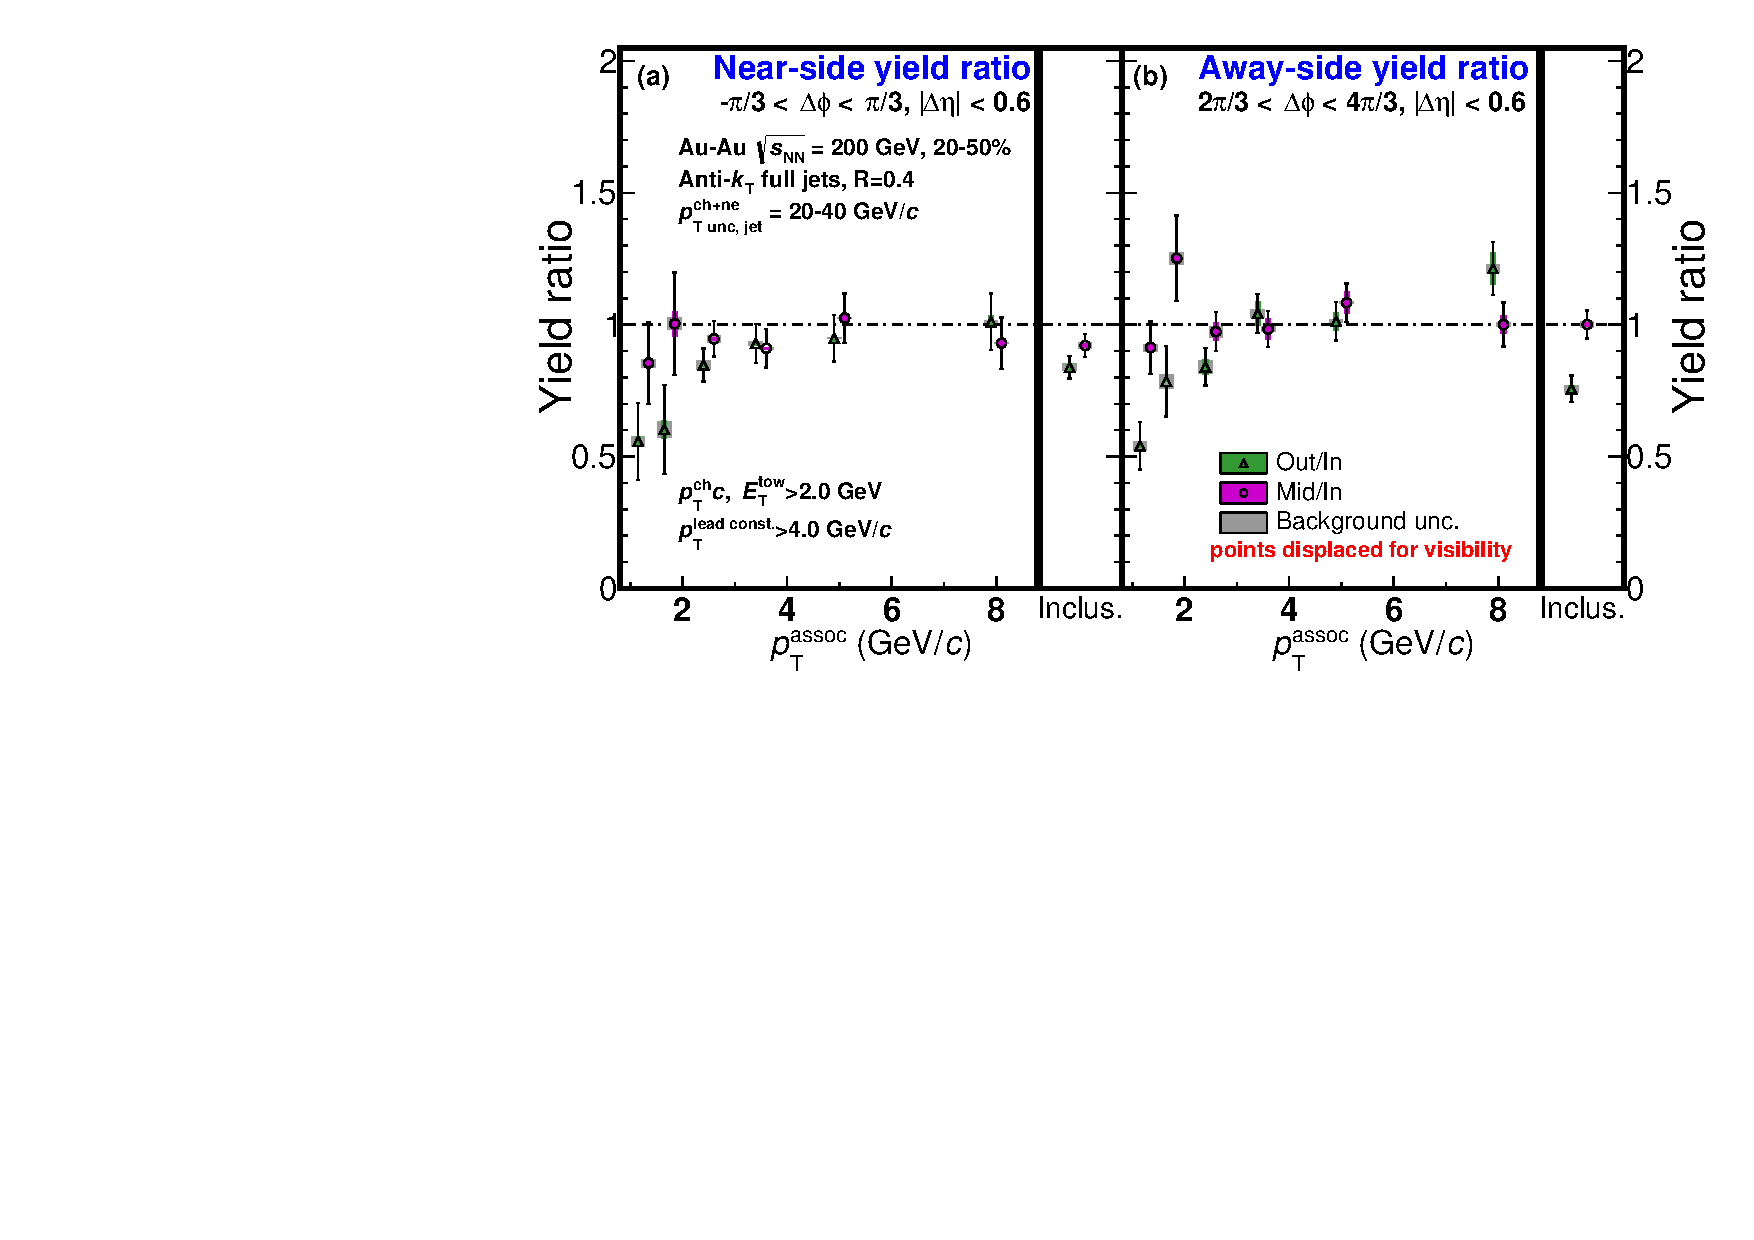
\includegraphics[height=0.6\textheight]{JHC/results/YieldRatio_J20-40_C20-50_wJEScorr.pdf}}
	\begin{itemize}\setlength{\itemsep}{0pt}\scriptsize
		\item 20--40~GeV/\(c\) jets. Yields, widths: \textbf{no event-plane dependence}
		\item<2-> Ratios \(\approx 1\); hint only in inclusive 1--10~GeV/\(c\) bin
		\item<3-> JEWEL: high \(p_\mathrm{T,assoc}\) w/o recoils, low with
	\end{itemize}
	\refnote{STAR, PRC 109 (2024) 044909}
\end{frame}

\begin{frame}{Jet-hadron correlations: conclusions}
	\begin{itemize}
		\item Yields, widths: \textbf{no event-plane dependence} within precision
		\item Path-length dependence \textbf{\(<\) uncertainties}
		\item Consistent with RHIC h-h, LHC jet-h
		\item Models need tuning for hard-fragmenting (biased) jets
	\end{itemize}
	\vspace{3mm}
	\begin{block}{Published}
		STAR, PRC \textbf{109}, 044909 (2024); HEPData ins2735142
	\end{block}
\end{frame}

%======================================================================
\section{Angularities of jets in Au+Au collisions}

\begin{frame}{Generalized angularities}
	\[
		\lambda^\kappa_\beta = \sum_{\mathrm{cons} \in \mathrm{jet}} z_\mathrm{cons}^\kappa \left(\frac{\Delta R_\mathrm{cons, jet}}{R}\right)^\beta ,
		\qquad z_\mathrm{cons} = \frac{p_\mathrm{T, cons}}{p_\mathrm{T, jet}}
	\]
	\begin{columns}[T]
		\begin{column}{0.56\textwidth}
			\begin{itemize}
				\item<2-> \(\kappa\): hard constituents; \(\beta\): wide angles
				\item<3-> \(\kappa = 1\), IRC safe: \(\lambda^1_{0.5}\) (LHA), \(\lambda^1_1\) (girth), \(\lambda^1_2\) (thrust \(\approx m^2/p_\mathrm{T}^2\))
				\item<4-> Au+Au: \(g = \lambda^1_1\), \(p_\mathrm{T}^D = \sqrt{\lambda^2_0}\), LeSub \(= p_\mathrm{T}^\mathrm{lead} - p_\mathrm{T}^\mathrm{sublead}\); hard-core jets, 0--20\% vs 40--80\%
				\item<5-> \textbf{MultiFold}: \alert{first unbinned ML unfolding in heavy ions}
			\end{itemize}
		\end{column}
		\begin{column}{0.42\textwidth}
			\centering
			\onslide<2->{%
				% same toy jet in the eta-phi plane (circle = jet radius R), marker area ~ constituent weight
				\begin{tikzpicture}[scale=0.95]
					\useasboundingbox (-1.1,-3.95) rectangle (3.5,1.05); % same frame for both stages
					% clicks 2-3: IRC-safe angularities, area ~ z (dR/R)^beta, normalised per panel
					\only<2-3>{%
						\begin{scope}[shift={(0,0)}]
							\draw[thin, gray] (0,0) circle (1);
							\draw[densely dotted, gray] (0,0) -- (1,0);
							\fill[PrimaryColor] (0,0) circle (0.8pt);
							\foreach \r/\a/\s in {0.060/35/0.300, 0.180/215/0.272, 0.320/115/0.244, 0.480/300/0.220, 0.660/65/0.223, 0.820/165/0.218, 0.940/250/0.206} \fill[blue!60!black, opacity=0.75] (\a:\r) circle (\s);
							\node[font=\scriptsize, anchor=north] at (0,-1.02) {\(\lambda^1_{0.5}\) LHA};
						\end{scope}
						\begin{scope}[shift={(2.4,0)}]
							\draw[thin, gray] (0,0) circle (1);
							\draw[densely dotted, gray] (0,0) -- (1,0);
							\fill[PrimaryColor] (0,0) circle (0.8pt);
							\foreach \r/\a/\s in {0.060/35/0.215, 0.180/215/0.257, 0.320/115/0.265, 0.480/300/0.265, 0.660/65/0.291, 0.820/165/0.300, 0.940/250/0.293} \fill[blue!60!black, opacity=0.75] (\a:\r) circle (\s);
							\node[font=\scriptsize, anchor=north] at (0,-1.02) {\(\lambda^1_1\) girth};
						\end{scope}
						\begin{scope}[shift={(1.2,-2.6)}]
							\draw[thin, gray] (0,0) circle (1);
							\draw[densely dotted, gray] (0,0) -- (1,0);
							\fill[PrimaryColor] (0,0) circle (0.8pt);
							\foreach \r/\a/\s in {0.060/35/0.055, 0.180/215/0.115, 0.320/115/0.158, 0.480/300/0.194, 0.660/65/0.249, 0.820/165/0.287, 0.940/250/0.300} \fill[blue!60!black, opacity=0.75] (\a:\r) circle (\s);
							\node[font=\scriptsize, anchor=north] at (0,-1.02) {\(\lambda^1_2\) thrust};
						\end{scope}
					}%
					% click 4 on: p_T^D = sqrt(lambda^2_0), area ~ z^2 on a common scale
					\only<4->{%
					\begin{scope}[shift={(0,0)}]
						\draw[thin, gray] (0,0) circle (1);
						\draw[densely dotted, gray] (0,0) -- (1,0);
						\fill[PrimaryColor] (0,0) circle (0.8pt);
						\foreach \r/\a/\s in {0.090/20/0.050, 0.220/140/0.046, 0.300/260/0.042, 0.410/75/0.042, 0.500/200/0.038, 0.580/320/0.038, 0.670/110/0.034, 0.740/30/0.034, 0.830/240/0.029, 0.900/170/0.029, 0.950/300/0.038} \fill[blue!60!black, opacity=0.75] (\a:\r) circle (\s);
						\node[font=\scriptsize, anchor=north] at (0,-1.02) {low \(p_\mathrm{T}^D = 0.31\)};
					\end{scope}
					\begin{scope}[shift={(2.4,0)}]
						\draw[thin, gray] (0,0) circle (1);
						\draw[densely dotted, gray] (0,0) -- (1,0);
						\fill[PrimaryColor] (0,0) circle (0.8pt);
						\foreach \r/\a/\s in {0.050/40/0.294, 0.350/200/0.042, 0.550/110/0.034, 0.750/290/0.025, 0.900/170/0.025} \fill[blue!60!black, opacity=0.75] (\a:\r) circle (\s);
						\node[font=\scriptsize, anchor=north] at (0,-1.02) {high \(p_\mathrm{T}^D = 0.72\)};
					\end{scope}
					% LeSub: leading minus subleading constituent, in a cone jet (\jetcone from TikzDiagrams.tex)
					\coordinate (lsA) at (-0.8,-2.75);
					\coordinate (lsB) at (3.1,-2.75);
					\jetcone{lsA}{lsB}{0.7}{0.16}
					\draw[-{Stealth[length=2.2mm]}, line width=1.6pt, red!80!black] (lsA) -- (2.3,-2.5) node[pos=0.55, above, sloped, font=\scriptsize, text=red!80!black, inner sep=1pt] {\(p_\mathrm{T}^\mathrm{lead}\)};
					\draw[-{Stealth[length=1.8mm]}, line width=1.1pt, orange!90!black] (lsA) -- (1.6,-3.05) node[pos=0.6, below, sloped, font=\scriptsize, text=orange!80!black, inner sep=1pt] {\(p_\mathrm{T}^\mathrm{sublead}\)};
					\foreach \e in {(1.0,-2.55),(0.9,-2.95),(1.2,-2.8)} \draw[-{Stealth[length=1.2mm]}, thin, white] (lsA) -- \e;
					\node[font=\scriptsize, anchor=north] at (1.2,-3.5) {LeSub \(= p_\mathrm{T}^\mathrm{lead} - p_\mathrm{T}^\mathrm{sublead}\)};
					}%
				\end{tikzpicture}}
		\end{column}
	\end{columns}
\end{frame}

\begin{frame}{Au+Au angularities: results}
	\centering
	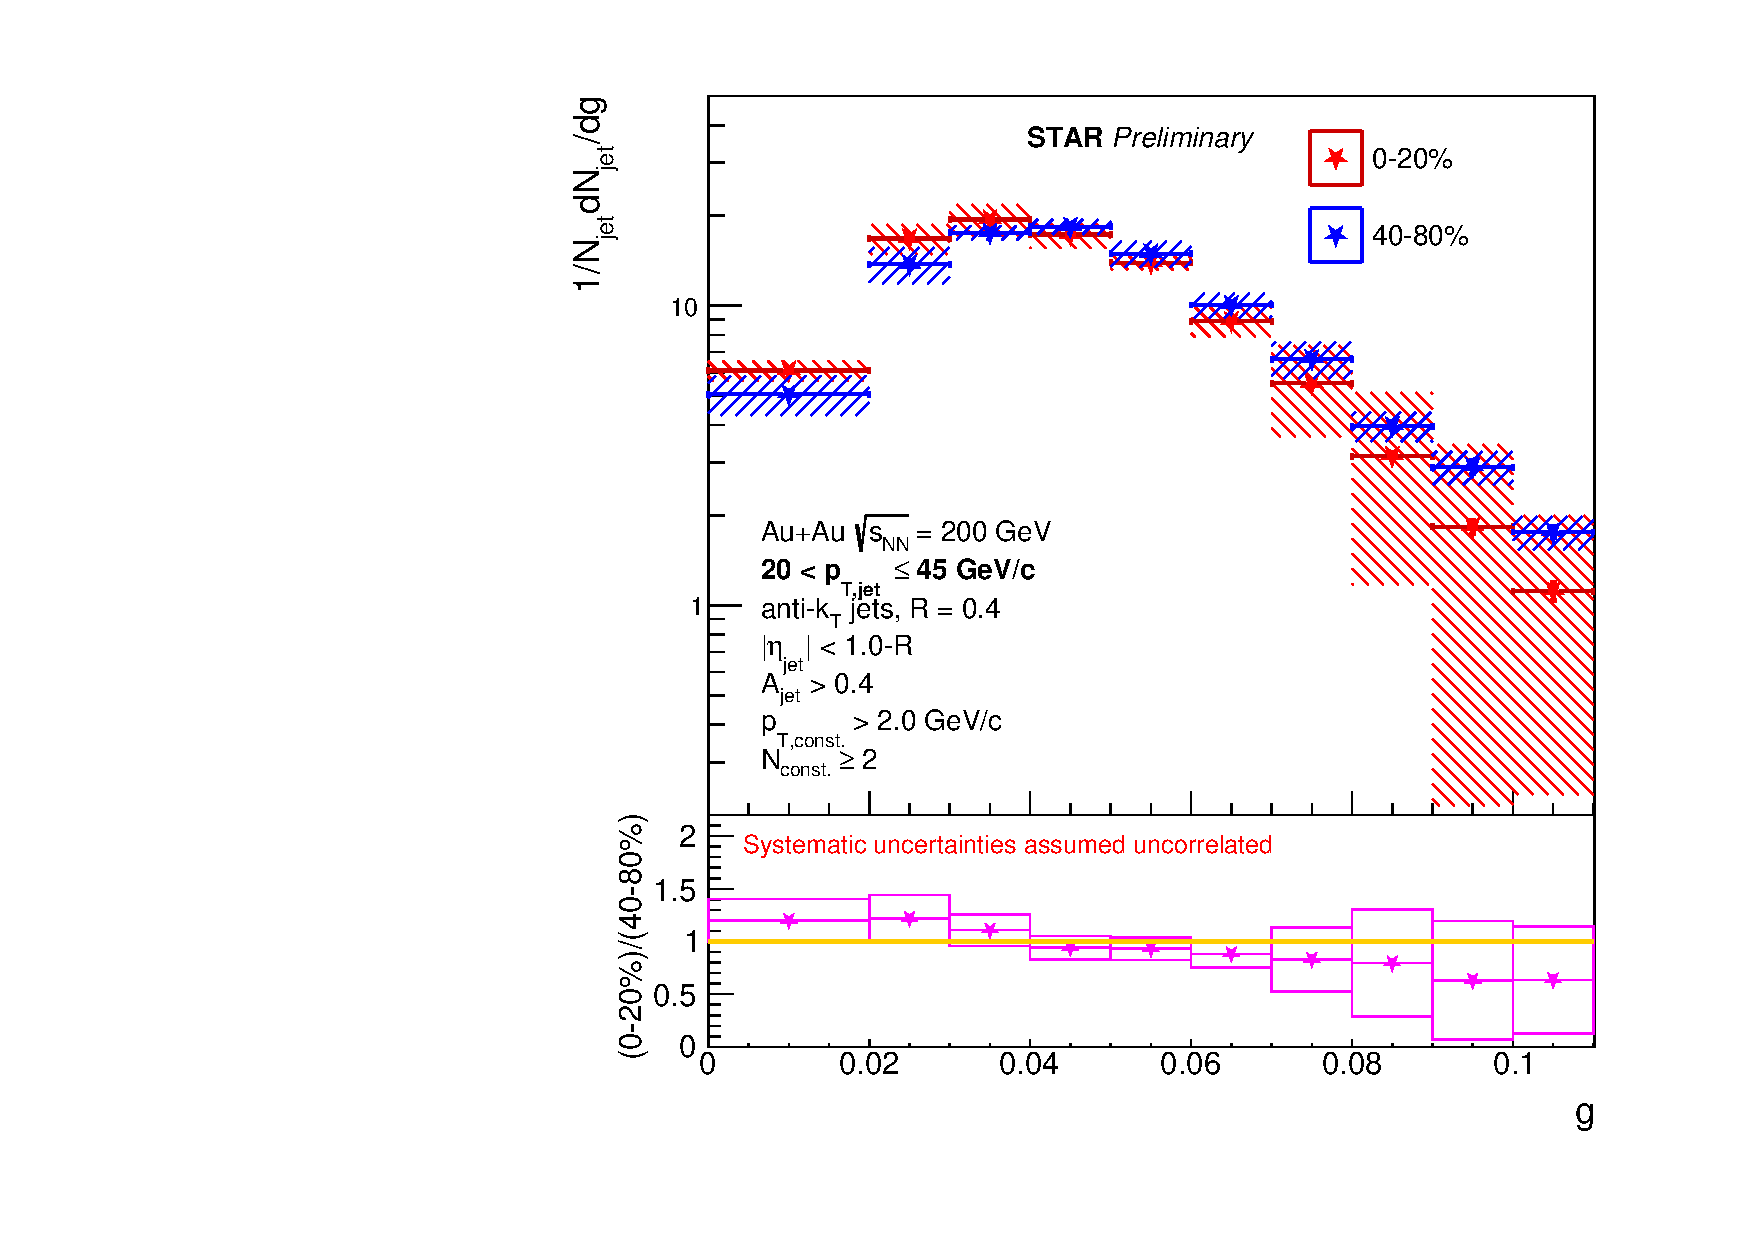
\includegraphics[width=0.325\linewidth]{angularities/AuAu/finalPlots_noPP_Girth_1_v3_warn.pdf}
	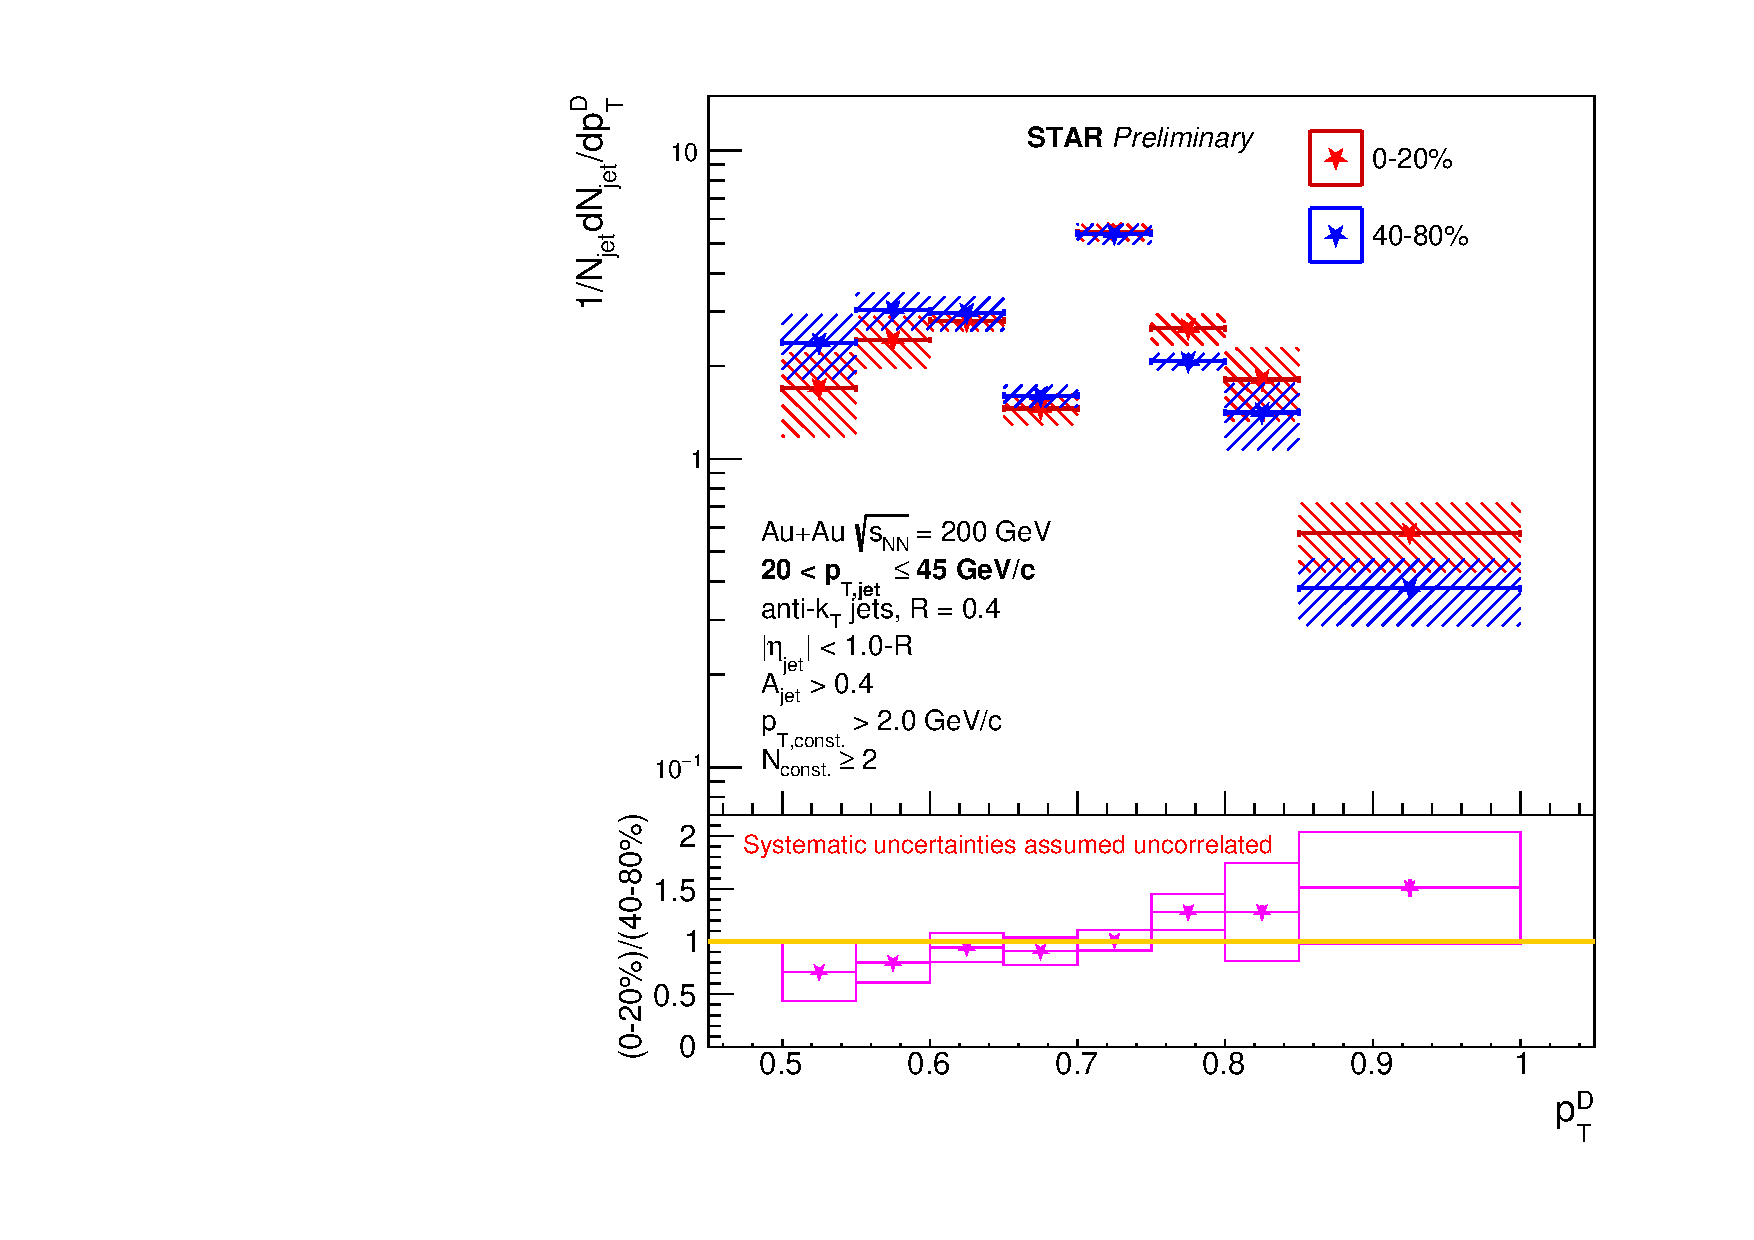
\includegraphics[width=0.325\linewidth]{angularities/AuAu/finalPlots_noPP_PtD_1_v3_warn.pdf}
	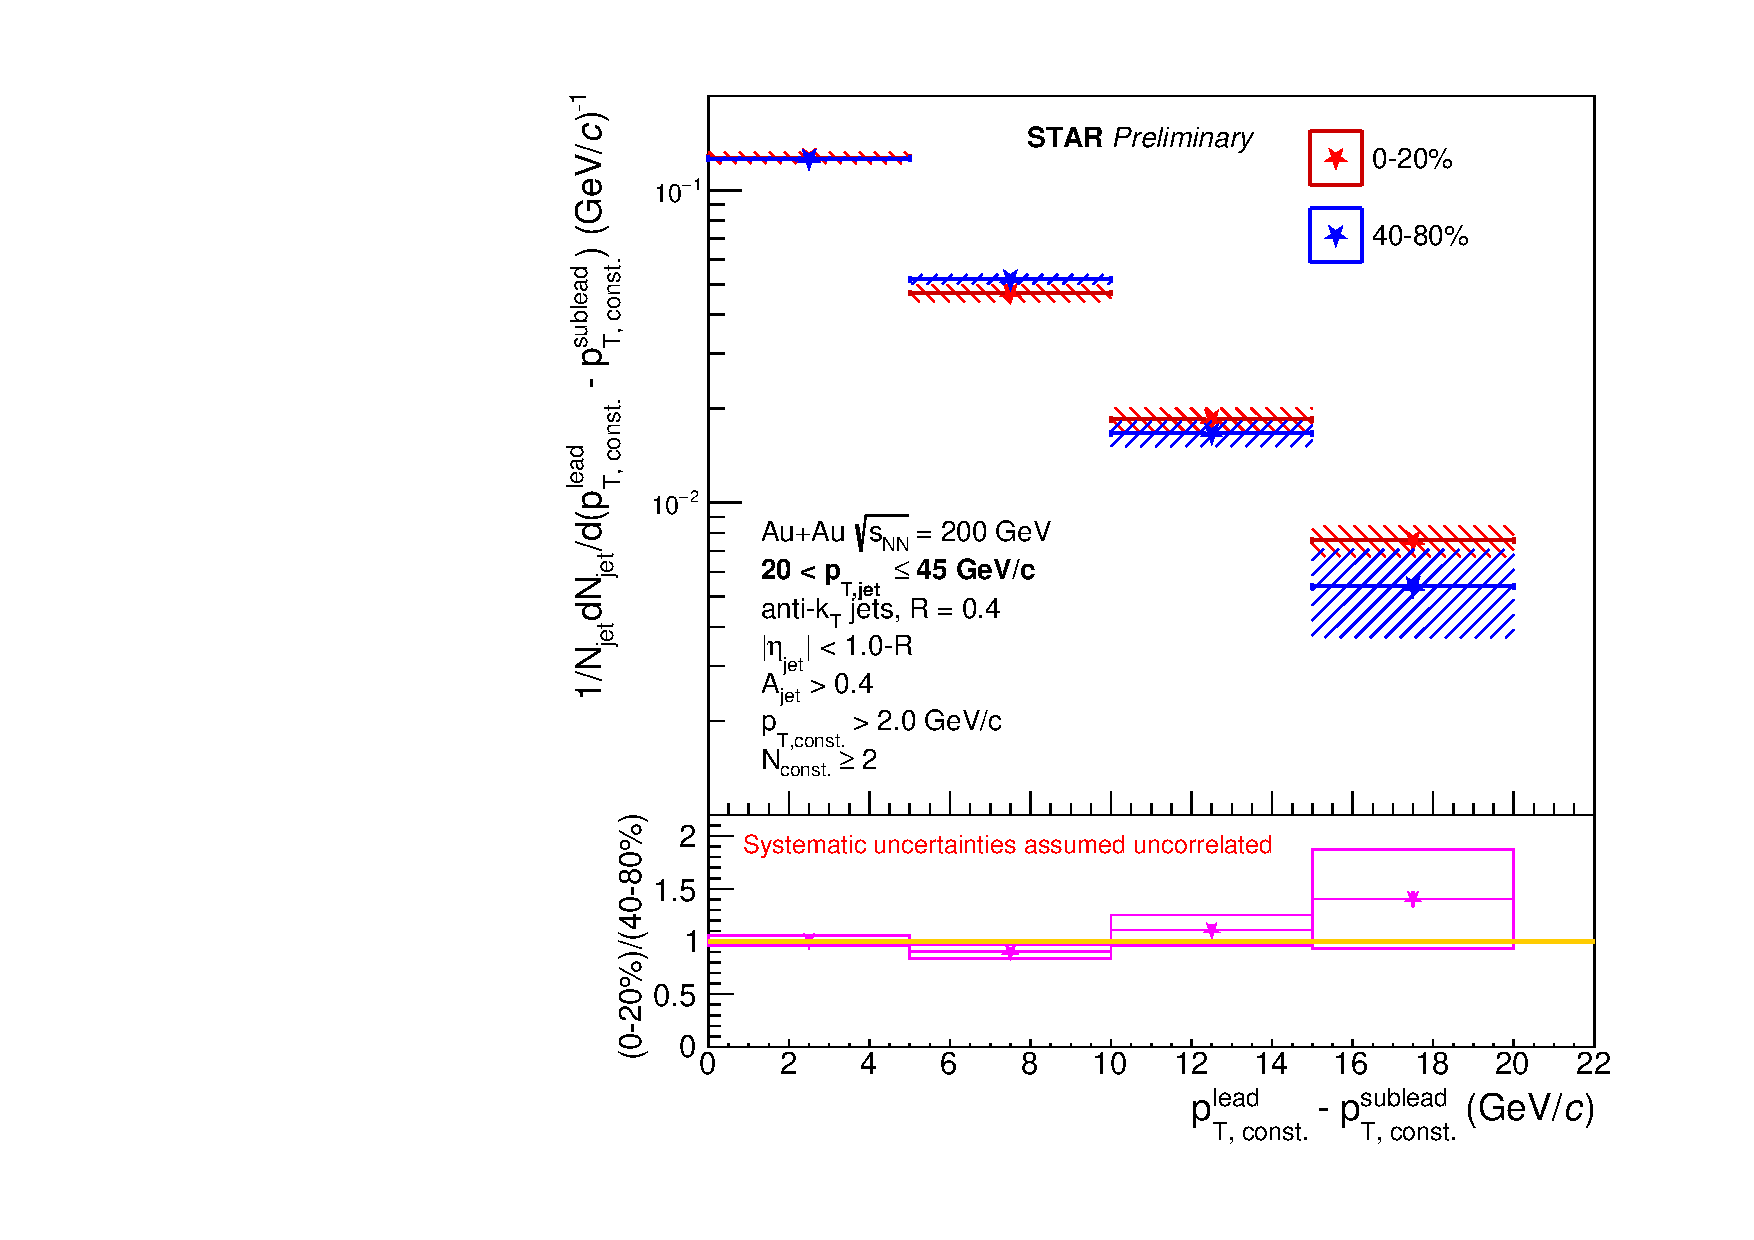
\includegraphics[width=0.325\linewidth]{angularities/AuAu/finalPlots_noPP_LeSub_1_v3_warn.pdf}
	\begin{itemize}\setlength{\itemsep}{0pt}
		\scriptsize
		\item 20--45~GeV/\(c\): central (red) \(\approx\) peripheral (blue)
		\item<2-> Hard-core cut \(\Rightarrow\) narrow jets, unresolved by QGP
		\item<3-> Next: \alert{grooming} instead of hard-core; develop unfolding in \alert{\(p+p\)}
	\end{itemize}
	\refnote{T.~Pani (STAR), QM 2023; HP 2024 (STAR Preliminary)}
\end{frame}

%======================================================================
\section{Inclusive and groomed angularities in \(p+p\)}

\begin{frame}{Inclusive and groomed angularities in \(p+p\): goals}
	\begin{enumerate}
		\item \textbf{Baseline} for heavy-ion angularities at 200~GeV
		\item<2-> Develop \textbf{unbinned unfolding} for RHIC
		\item<3-> Go \textbf{beyond distributions}
	\end{enumerate}
	\vspace{4mm}
	\onslide<4->{
		Measured: \lam{\beta}, \(\beta = 0.5, 1, 2\), inclusive + groomed; \(\langle\lambda_\beta\rangle\) vs \Rg}
	\refnote{T.~Pani (STAR), HP 2026 (STAR Preliminary)}
\end{frame}

\begin{frame}{SoftDrop grooming}
	\begin{columns}[c]
		\begin{column}{0.59\textwidth}
			\centering
			\resizebox{\linewidth}{!}{%
				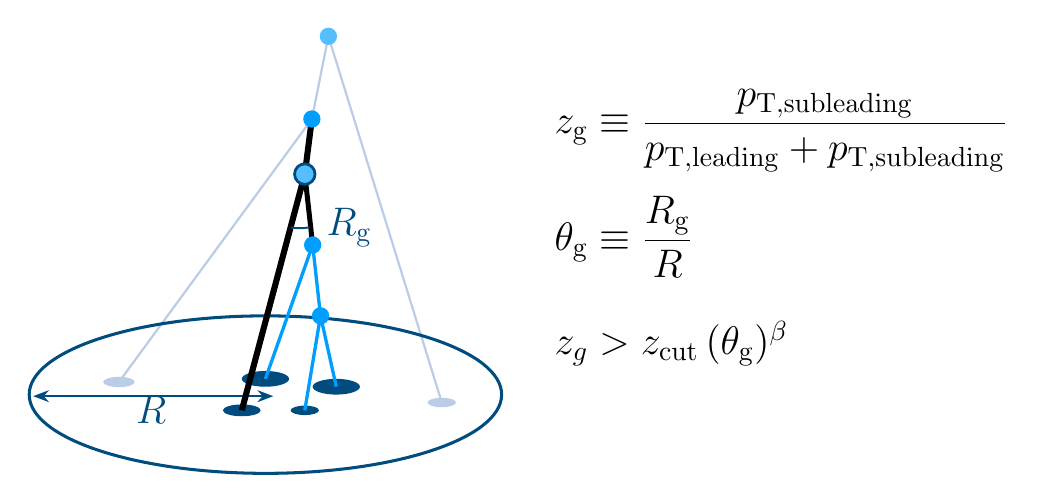
\begin{tikzpicture}[font=\Large, >={Stealth[length=2mm]}, baseline]
					\coordinate (O)  at (0,0);
					\coordinate (A)  at (0.80,4.55);
					\coordinate (D)  at (0.59,3.50);
					\coordinate (N)  at (0.5,2.8);
					\coordinate (S1) at (0.6, 1.9);
					\coordinate (S2) at (0.7,1.);
					\coordinate (Fc) at (-0.3,-0.2);
					\coordinate (F1) at (0.0,0.2);
					\coordinate (F2) at (0.5,-0.2);
					\coordinate (F3) at (0.9,0.1);
					\coordinate (FL) at (-1.86,0.16);
					\coordinate (FR) at (2.24,-0.1);
					\draw[sdlight, line width=0.8pt] (A) -- (D);
					\draw[sdlight, line width=0.8pt] (D) -- (FL);
					\draw[sdlight, line width=0.8pt] (A) -- (FR);
					\draw[sdnavy, line width=1.1pt] (O) ellipse [x radius=3, y radius=1.0];
					\draw[{Stealth[length=2mm]}-{Stealth[length=2mm]}, sdnavy, line width=0.9pt] (-2.95, -0.02) -- (0.1, -0.02);
					\node[sdnavy, below] at (-1.45,0.1) {$R$};
					\fill[sdlight] (FL) ellipse [x radius=0.20, y radius=0.065];
					\fill[sdnavy]  (Fc) ellipse [x radius=0.24, y radius=0.075];
					\fill[sdnavy]  (F1) ellipse [x radius=0.3, y radius=0.1];
					\fill[sdnavy]  (F2) ellipse [x radius=0.18, y radius=0.060];
					\fill[sdnavy]  (F3) ellipse [x radius=0.3, y radius=0.1];
					\fill[sdlight] (FR) ellipse [x radius=0.18, y radius=0.060];
					\draw[black,  line width=2.2pt] (Fc) -- (N) -- (D);
					\draw[black, line width=1.8pt] (N) -- (S1);
					\draw[sdblue,  line width=1.2pt] (S1) -- (F1);
					\draw[sdblue,  line width=1.2pt] (S1) -- (S2);
					\draw[sdblue, line width=1.2pt] (S2) -- (F2);
					\draw[sdblue, line width=1.2pt] (S2) -- (F3);
					\draw[sdnavy, line width=0.7pt] (N) ++(-105:0.7) arc (-100:-80.1:0.7);
					\node[sdnavy] at ($(N)+(-50:0.88)$) {$R_{\mathrm g}$};
					\fill[sdcyan] (A) circle (0.11);
					\fill[sdblue] (D) circle (0.11);
					\draw[sdnavy, line width=1pt, fill=sdcyan] (N) circle (0.13);
					\fill[sdblue] (S1) circle (0.11);
					\fill[sdblue] (S2) circle (0.11);
					\node[anchor=west] at (3.55,3.35)
					{$z_{\mathrm g}\equiv\dfrac{p_{\mathrm{T,subleading}}}{p_{\mathrm{T,leading}}+p_{\mathrm{T,subleading}}}$};
					\node[anchor=west] at (3.55,2.0)
					{$\theta_{\mathrm g}\equiv\dfrac{R_{\mathrm g}}{R}$};
					\node[anchor=west] at (3.55,0.65)
					{$z_g > z_{\rm cut}\,(\theta_{\mathrm{g}})^{\beta}$};
				\end{tikzpicture}}
		\end{column}
		\begin{column}{0.39\textwidth}
			\small
			\begin{itemize}
				\item C/A recluster \(\Rightarrow\) angle-ordered tree
				\item<2-> Unwind; drop softer branch until \(z > z_\mathrm{cut}\,\theta^\beta\)
				\item<3-> First hard splitting \(\to\) \zg, \Rg
				\item<4-> \(z_\mathrm{cut} = 0.2\), \(\beta = 0\)
			\end{itemize}
		\end{column}
	\end{columns}
	\refnote{Larkoski, Marzani, Soyez, Thaler, JHEP 05 (2014) 146}
\end{frame}

\begin{frame}{What \Rg tells us}
	\centering
	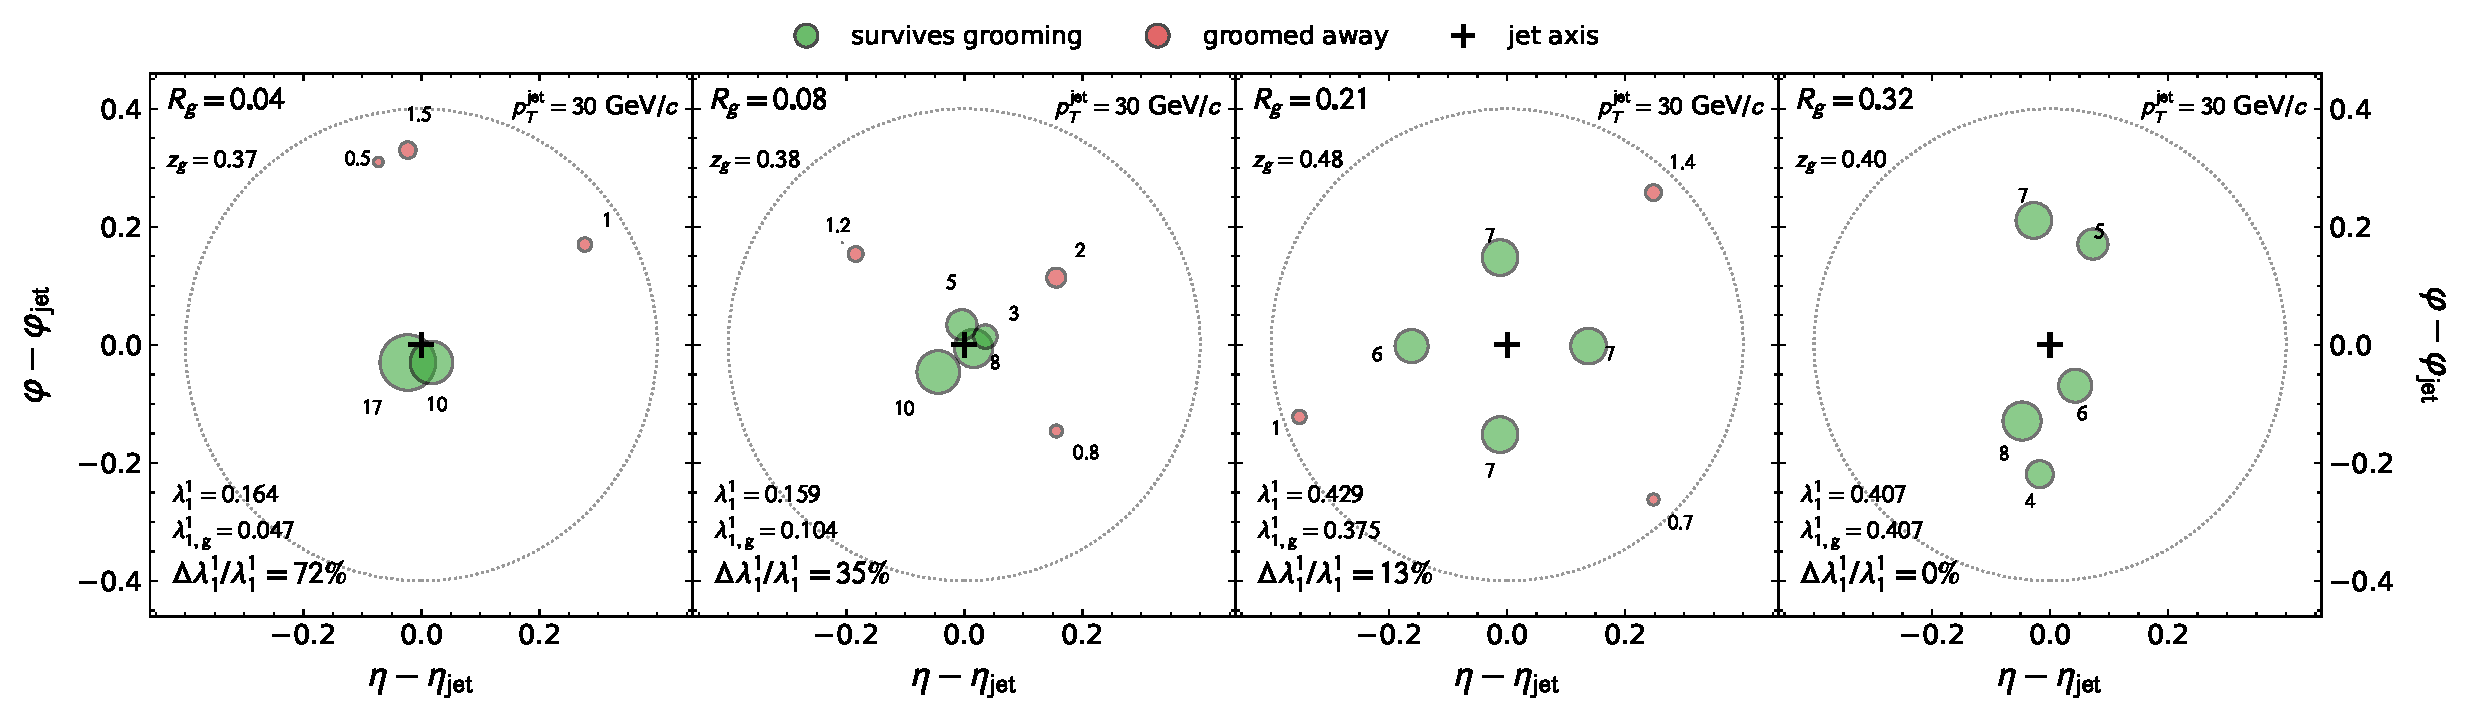
\includegraphics[width=0.95\linewidth]{fig_grooming_cartoon_4panel.pdf}
	\begin{itemize}
		\item Larger \Rg: earlier splitting, more room for later ones
		\item<2-> Groomed-away girth \(\downarrow\) with \Rg: pencil \(\to\) two-prong
		\item<3-> \(\langle\lambda_\beta\rangle\) vs \Rg: radiation \alert{at fixed splitting angle}
	\end{itemize}
\end{frame}

\begin{frame}{Embedding: from particles to the detector}
	\centering
	% fig:UnfoldingScheme from appendices/unfolding.tex (TikZ copied verbatim)
	\resizebox{!}{0.82\textheight}{%
		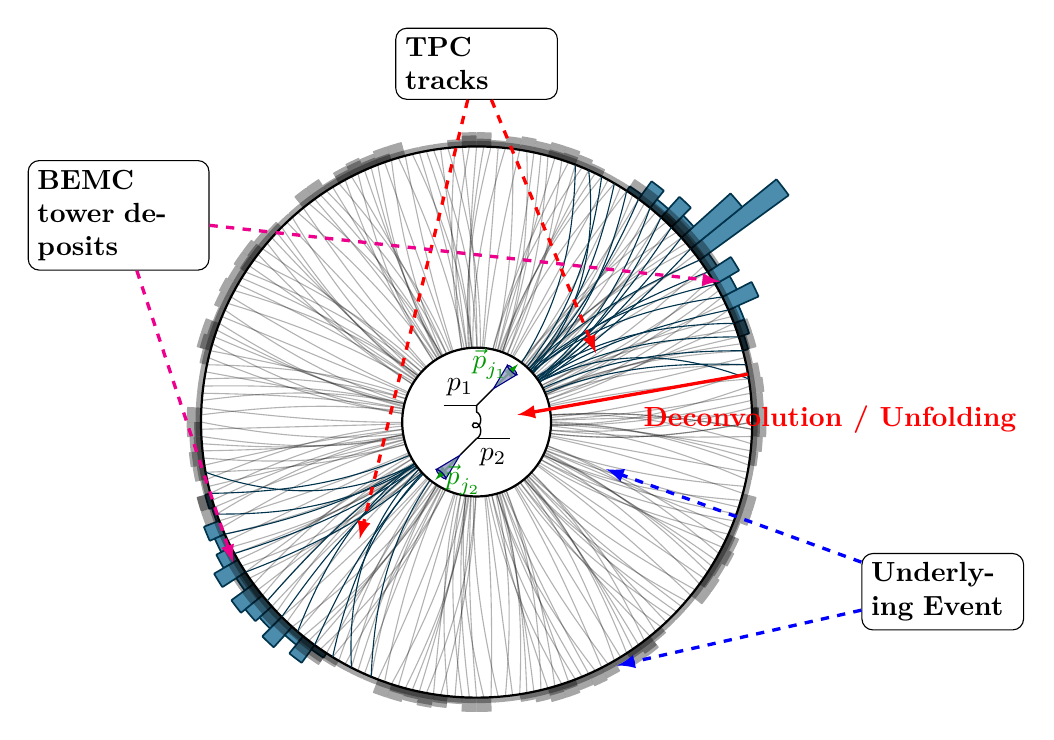
\begin{tikzpicture}[scale=0.7,rotate=0]
			\def\R{5} % tracker outer radius
			\def\dang{3} % angular granularity of calo deposits, 
			% HCAL DEPOSITS
			\foreach \dr [count=\i,
				evaluate={\r=\R+\dr; \anga=12+\dang*\i; \angb=\anga+\dang;}
			] in {0.1, 0.2, 0.2, 0.6, 0.3,0.5,0.2,2.0,1.2,0.3,0.5, 0.2, 0.4, 0.1}{
					\draw[calo] (0,0) -- (\anga:\r) arc(\anga:\angb:\r) -- cycle;
					%\draw[calo]
					%  (\anga:\R) -- (\anga:\r) arc(\anga:\angb:\r)
					%  -- (\angb:\R) arc(\angb:\anga:\R) -- cycle;
				}

			\foreach \dr [count=\i,
				evaluate={\r=\R+\dr; \anga=192+\dang*\i; \angb=\anga+\dang;}
			] in {0.1, 0.05, 0.3, 0.2,0.3,0.5,0.2, 0.5,0.4,0.3,0.5, 0.2, 0.4, 0.1}{
					\draw[calo] (0,0) -- (\anga:\r) arc(\anga:\angb:\r) -- cycle;
					%\draw[calo]
					%  (\anga:\R) -- (\anga:\r) arc(\anga:\angb:\r)
					%  -- (\angb:\R) arc(\angb:\anga:\R) -- cycle;
				}

			\foreach \ang [count=\i,
				evaluate={\stepa = 15;
						\stepb=\stepa+50;
						\ra=\R+0.25*sin(\dang*\i*10);
						\rb=\R+0.2*cos(\dang*\i*15);
						\rc=\R+0.3*sin(\dang*\i*20);
						\rd=\R+0.1;
					}]in {0, 3,...,360}{
			\draw[calobg] (0,0) -- (\ang:\ra) arc(\ang:\ang+\dang:\ra) -- cycle;
			\draw[calobg] (0,0) -- (\ang:\rd) arc(\ang:\ang+\dang:\rd) -- cycle;
			\draw[calobg] (0,0) -- (\stepa*\dang+\ang:\rb) arc(\stepa*\dang+\ang:\stepa*\dang+\ang+\dang:\rb) -- cycle;
			\draw[calobg] (0,0) -- (\stepb*\dang+\ang:\rc) arc(\stepb*\dang+\ang:\stepb*\dang+\ang+\dang:\rc) -- cycle;
			}

			\draw[thick,fill=white] (0,0) circle(\R);

			\foreach \ang [count=\i,
				evaluate={\bend=12*sin(20+\i*\dang*15)}]in {0, 3,...,360}{
			\draw[black,opacity=0.3,thin,fill=none]
			(0,0) to[bend right=\bend] (\ang:\R);
			}

			\foreach \ang [count=\i,
				evaluate={\bend=12*cos(\i*\dang*15)}]in {0, 3,...,360}{
			\draw[black,opacity=0.3,thin,fill=none]
			(0,0) to[bend left=\bend] (\ang-\dang*0.5:\R);
			}

			%\draw[calo]
			%  (\anga:\R) -- (\anga:\r) arc(\anga:\angb:\r)
			%  -- (\angb:\R) arc(\angb:\anga:\R) -- cycle;

			\foreach \bend [count=\i,
				evaluate={\anga=6+\dang*\i;}
			] in {30, 14, 15,18, 20, 12, 19, 17, 11, 12}{
					\draw[blue!60!green!50!black,thin,fill=none]
					(0,0) to[bend left=\bend] (\anga:\R);
				}

			\foreach \bend [count=\i,
				evaluate={\anga=72-\dang*\i;}
			] in {20, 30, 19, 18, 20, 12, 19, 17, 12, 10, 8}{
					\draw[blue!60!green!50!black,thin,fill=none]
					(0,0) to[bend right=\bend] (\anga:\R);
				}

			\foreach \bend [count=\i,
				evaluate={\anga=186+1.5*\dang*\i;}
			] in {30, 14, 20, 12, 11, 12}{
					\draw[blue!60!green!50!black,thin,fill=none]
					(0,0) to[bend left=\bend] (\anga:\R);
				}

			\foreach \bend [count=\i,
				evaluate={\anga=252-1.5*\dang*\i;}
			] in {20, 30, 19, 12, 19, 10, 8}{
					\draw[blue!60!green!50!black,thin,fill=none]
					(0,0) to[bend right=\bend] (\anga:\R);
				}

			\begin{scope}[visible on=<2->]
				\node[draw, text width=0.15\textwidth, rounded corners=4pt] (tracks) at (90:1.3*\R){
					\textbf{TPC tracks}
				};
				\draw (tracks) edge[dashed,  ->, very thick, red] (225:0.6*\R);
				\draw (tracks) edge[dashed,  ->, very thick, red] (30:0.5*\R);
			\end{scope}

			\begin{scope}[visible on=<3->]
				\node[draw, text width=0.17\textwidth, rounded corners=4pt] (towers) at (150:1.5*\R){
					\textbf{BEMC tower deposits}
				};
				\draw (towers) edge[dashed,  ->, very thick, magenta] (210:1.02*\R);
				\draw (towers) edge[dashed,  ->, very thick, magenta] (30:1.02*\R);
			\end{scope}

			\begin{scope}[visible on=<4->]
				\node[draw, text width=0.15\textwidth, rounded corners=4pt] (UE) at (340:1.8*\R){
					\textbf{Underlying Event}
				};
				\draw (UE) edge[dashed, ->, very thick, blue] (300:1.02*\R);
				\draw (UE) edge[dashed,  ->, very thick, blue] (340:0.5*\R);
			\end{scope}

			\draw[thick,fill=white] (0,0) circle(0.27*\R);
			\begin{feynhand}[scale=0.3]
				\vertex (a)  at (-1, -2);
				\vertex(b)  at (-2, 1);
				\vertex (c)  at (0, -1);
				\vertex (d)  at (0, 1);
				\propag [plain] (c) to (a);
				\propag [plain] (b) to  [edge label = $p_1$] (d);
				\propag [gluon] (c) to (d);
				\vertex(e) at (2, -1) ;
				\vertex (f) at (1, 2);
				\propag [plain] (e) to [edge label = $p_2$](c);
				\propag [plain] (d) to (f);
				\coordinate (J1) at (2.5,3.5);
				\coordinate (J2) at (-2.5, -3.5);
				\jetcone{f}{J1}{0.4}{0.10}
				\jetcone{a}{J2}{0.4}{0.10}
				\node[vector,left] at (J1) {$\vv{p}_{j_1}$};
				\node[vector,right] at (J2) {$\vv{p}_{j_2}$};
			\end{feynhand}

			\begin{scope}[visible on=<5->]
				\draw  (10:\R) edge["\textbf{Deconvolution / Unfolding}", ->, very thick, red] (10:0.15*\R);
			\end{scope}
		\end{tikzpicture}}
\end{frame}

\begin{frame}{Dataset and jets}
	\centering
	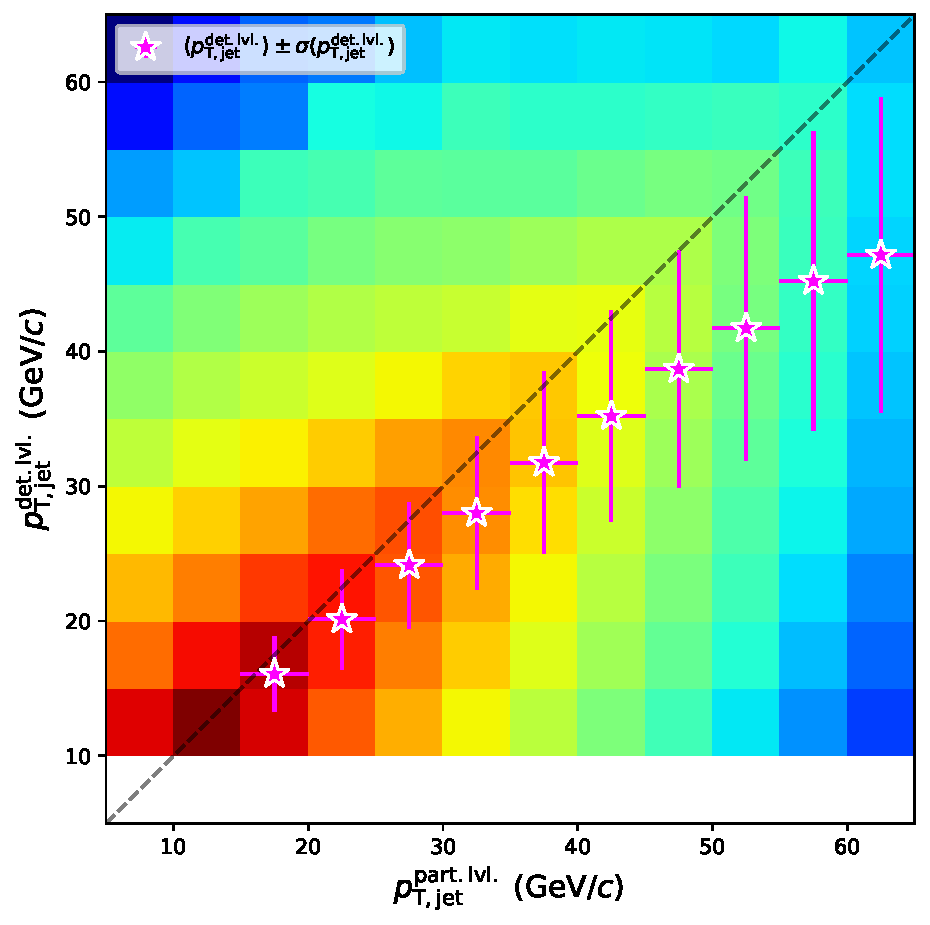
\includegraphics[width=0.285\linewidth]{jet_pt_response.pdf}\hfill
	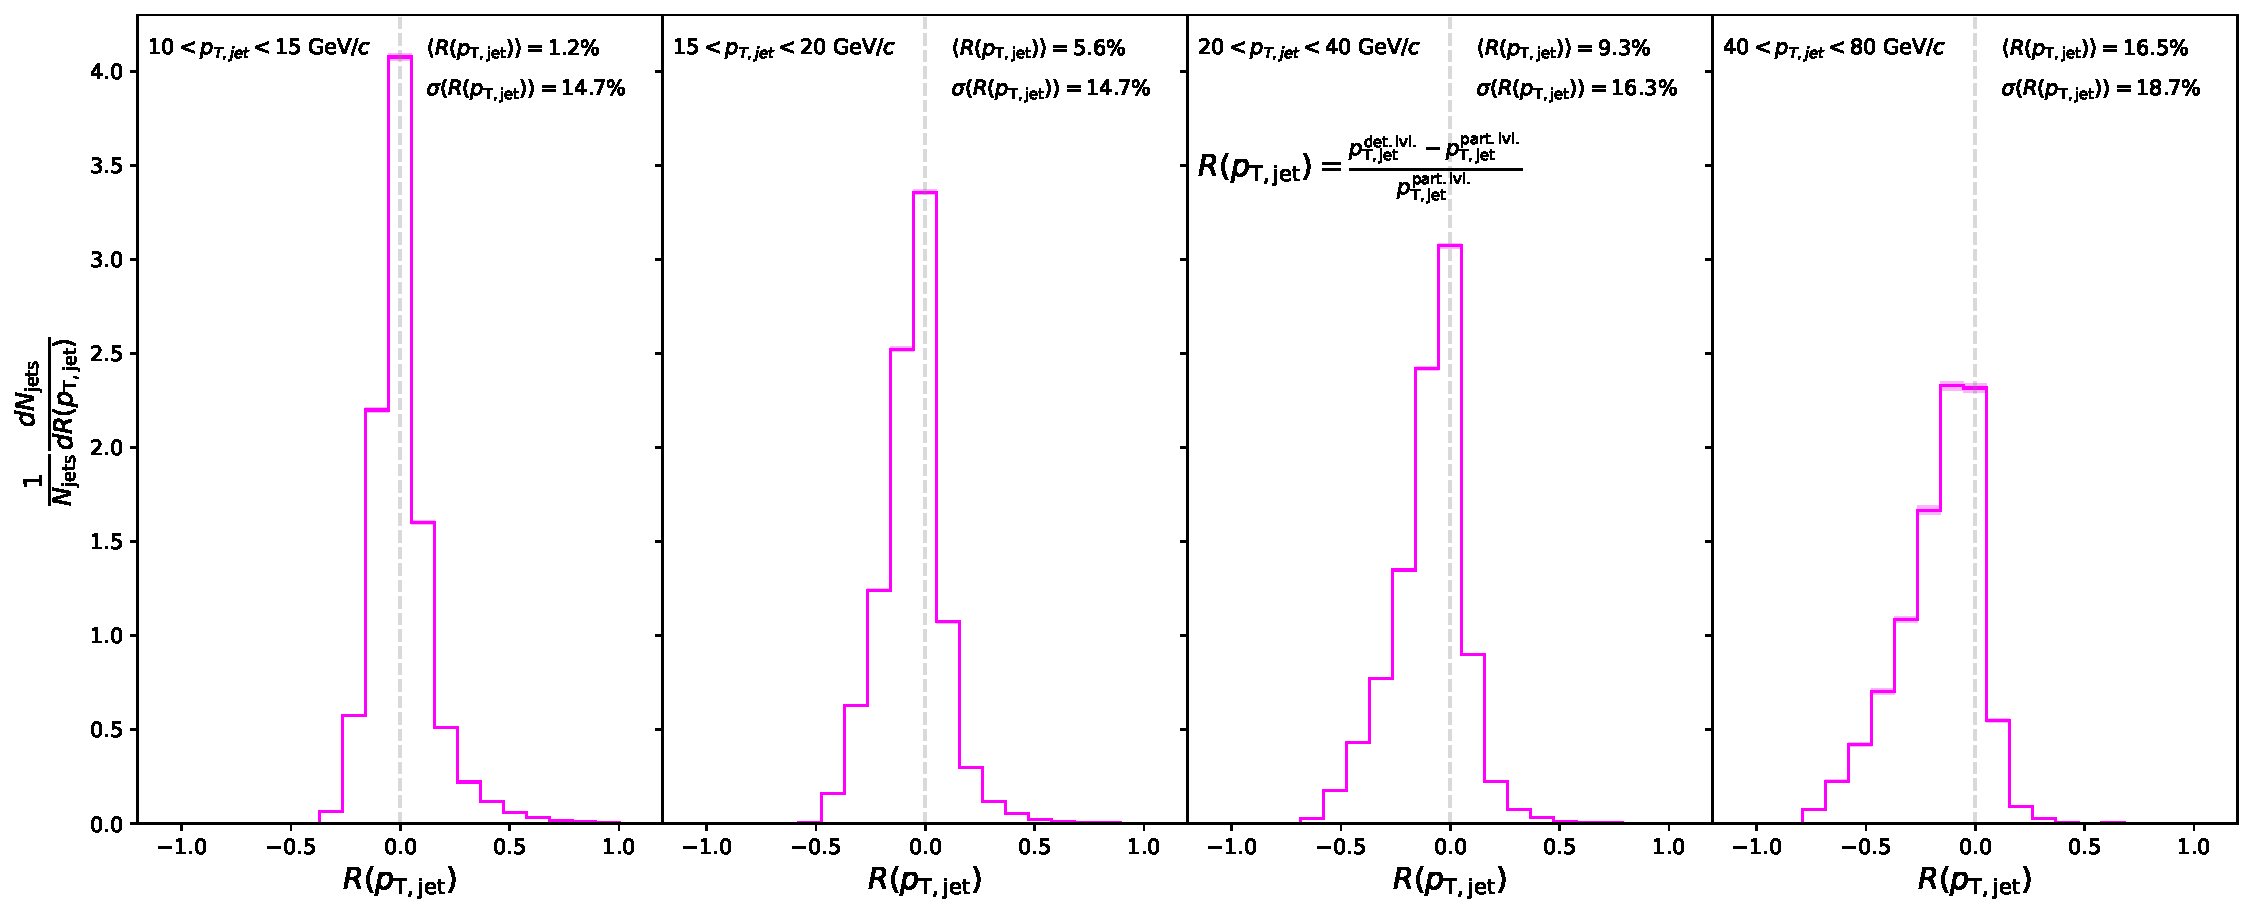
\includegraphics[width=0.7\linewidth]{jet_pt_res.pdf}
	\vfill
	\begin{columns}[T]
		\begin{column}{0.49\textwidth}
			\small
			\begin{itemize}
				\item \(p+p\) 200~GeV, 2012; 5.1M HT events
				\item Tracks, towers \(> 0.2\)~GeV; full hadronic corr.
				\item anti-\(k_\mathrm{T}\) \(R = 0.4\), \(|\eta| \leq 0.6\), \(p_\mathrm{T} \geq 10\)~GeV/\(c\), \(N_\mathrm{ch} \geq 2\)
			\end{itemize}
		\end{column}
		\begin{column}{0.49\textwidth}
			\small
			\begin{itemize}
				\item \textbf{Inclusive}: no hard-core cut
				\item Embedding: \PYsix + GEANT3 + zero-bias, 16M events
				\item JES shift 1\(\to\)17\%, JER 15\(\to\)19\% (low \(\to\) high \(p_\mathrm{T}\))
			\end{itemize}
		\end{column}
	\end{columns}
\end{frame}

\begin{frame}{Unbinned unfolding with MultiFold}
	\centering
	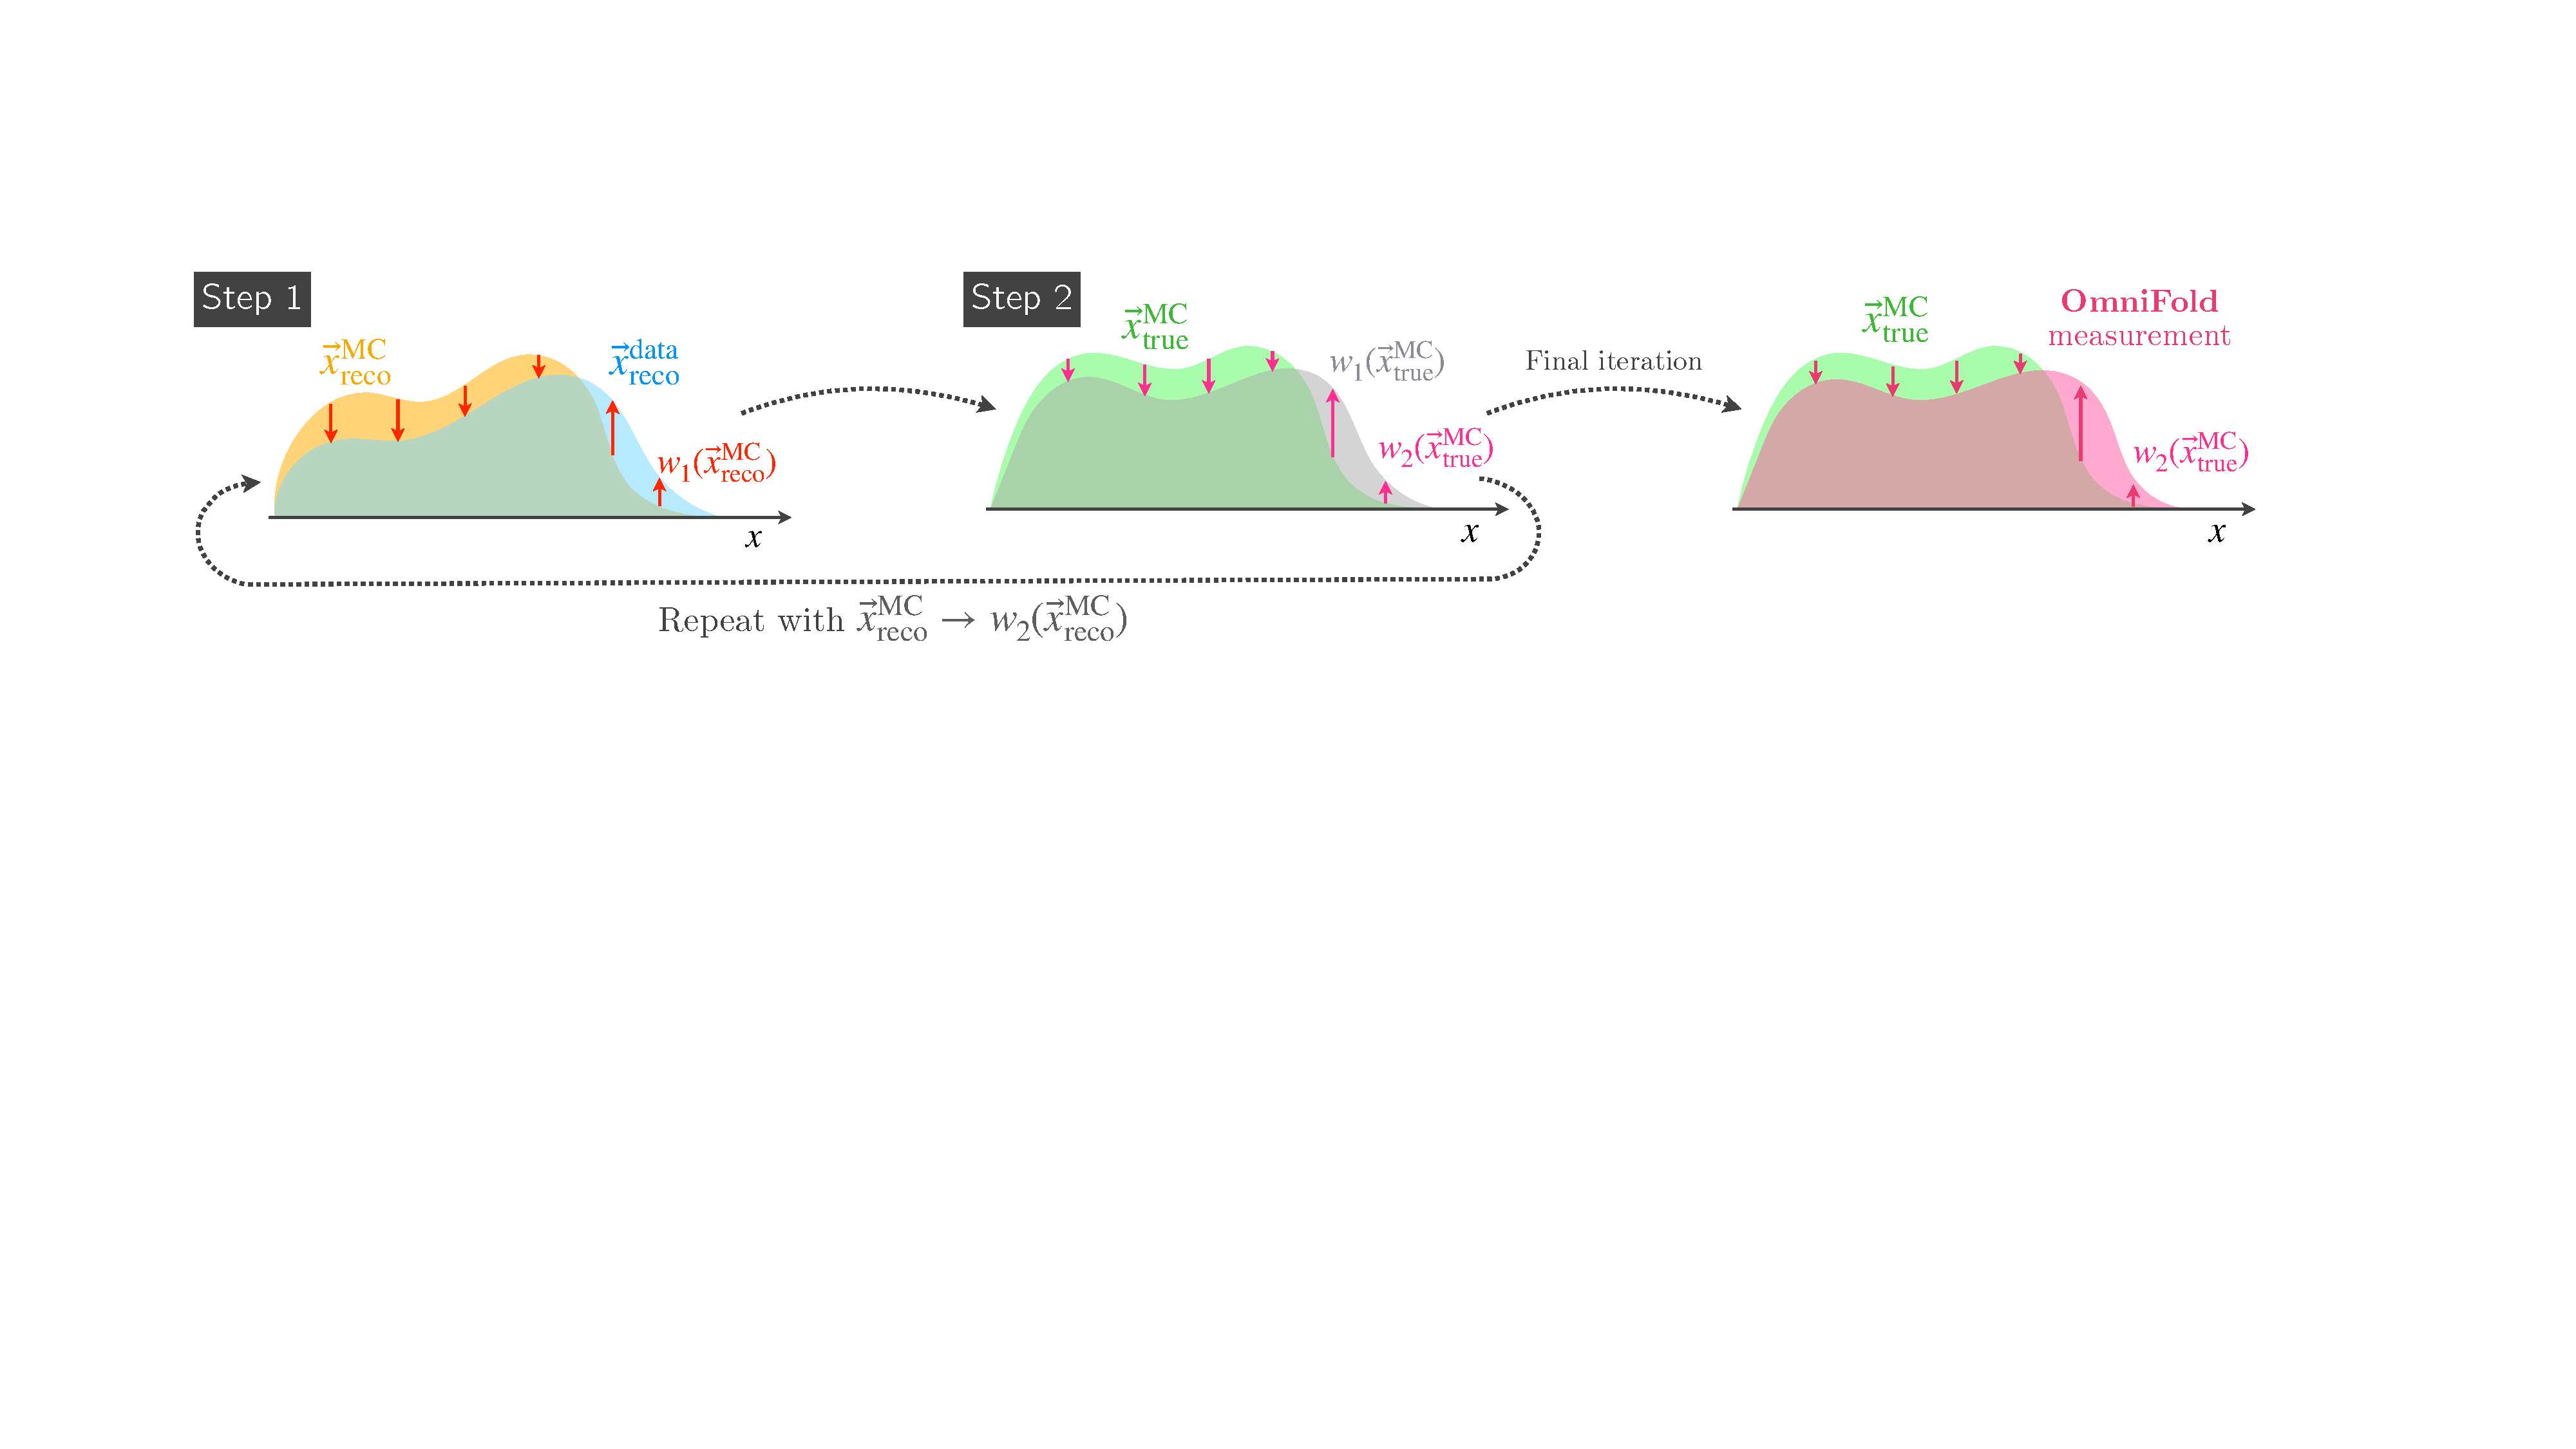
\includegraphics[width=\linewidth]{omnifold_fig_2025_04_24.pdf}
	\begin{columns}[T]
		\begin{column}{0.5\textwidth}
			\begin{itemize}
				\item IBU with histograms \(\to\) \textbf{classifiers}: \(\frac{f}{1-f} \approx \frac{p_A}{p_B}\)
				\item<2-> \textbf{Step 1}: reco \(\to\) data. \textbf{Step 2}: pull to gen, smooth
				\item<3-> \textbf{23 features}/jet \(\to\) weight/jet \(\Rightarrow\) any function of them, after the fact
			\end{itemize}
		\end{column}
		\begin{column}{0.46\textwidth}
			\begin{itemize}
				\item<4-> 4 classifiers: DNN 3\(\times\)256, AdamW; \textbf{2 iterations}
				\item<5-> \textbf{50 replicas} (500k+500k jets each) \(\Rightarrow\) stat.\ unc.\ = spread
				\item<5-> All on one GPU (\texttt{torchstrap})
			\end{itemize}
		\end{column}
	\end{columns}
	\refnote{Andreassen, Komiske, Metodiev, Nachman, Thaler, PRL 124 (2020) 182001}
\end{frame}

\begin{frame}{Training diagnostics}
	\begin{columns}[c]
		\begin{column}{0.59\textwidth}
			\centering
			% loss panels of the four classifiers (steps 1, 1b, 2, 2b), 2x2, from
			% jet-angularity-study/studies/plot_training.py (run metrics), training_loss_2x2.pdf
			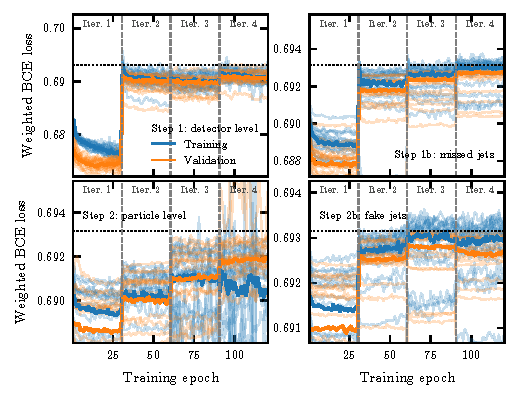
\includegraphics[width=\linewidth, height=0.8\textheight, keepaspectratio]{angularities/pp/unfolding/pp_multifold_training_loss.pdf}
		\end{column}
		\begin{column}{0.39\textwidth}
			{\footnotesize
				\[\begin{aligned}
						\mathcal{L}_\mathrm{BCE} & = -\frac{1}{\sum_i w_i}\sum_i w_i \big[\, y_i \ln f_i \\
						                         & \qquad + (1-y_i) \ln(1-f_i)\big]
					\end{aligned}\]
				\centering \(f_i = f(\mathbf{x}_i)\): classifier output, \(y_i \in \{0,1\}\)\par}
			\begin{itemize}
				\item Weighted BCE loss; thin lines = replicas
				\item<2-> Iter.\ 1: loss \(< \ln 2\) \(\Rightarrow\) data \(\ne\) reco
				\item<3-> Iter.\ 2+: loss \(\approx \ln 2\) \(\Rightarrow\) converged
				\item<4-> Later: replicas diverge \(\Rightarrow\) use \textbf{iter.\ 2}
			\end{itemize}
		\end{column}
	\end{columns}
\end{frame}

\begin{frame}{Closure with a data-like prior}
	\begin{columns}[c]
		\begin{column}{0.59\textwidth}
			\centering
			\only<1>{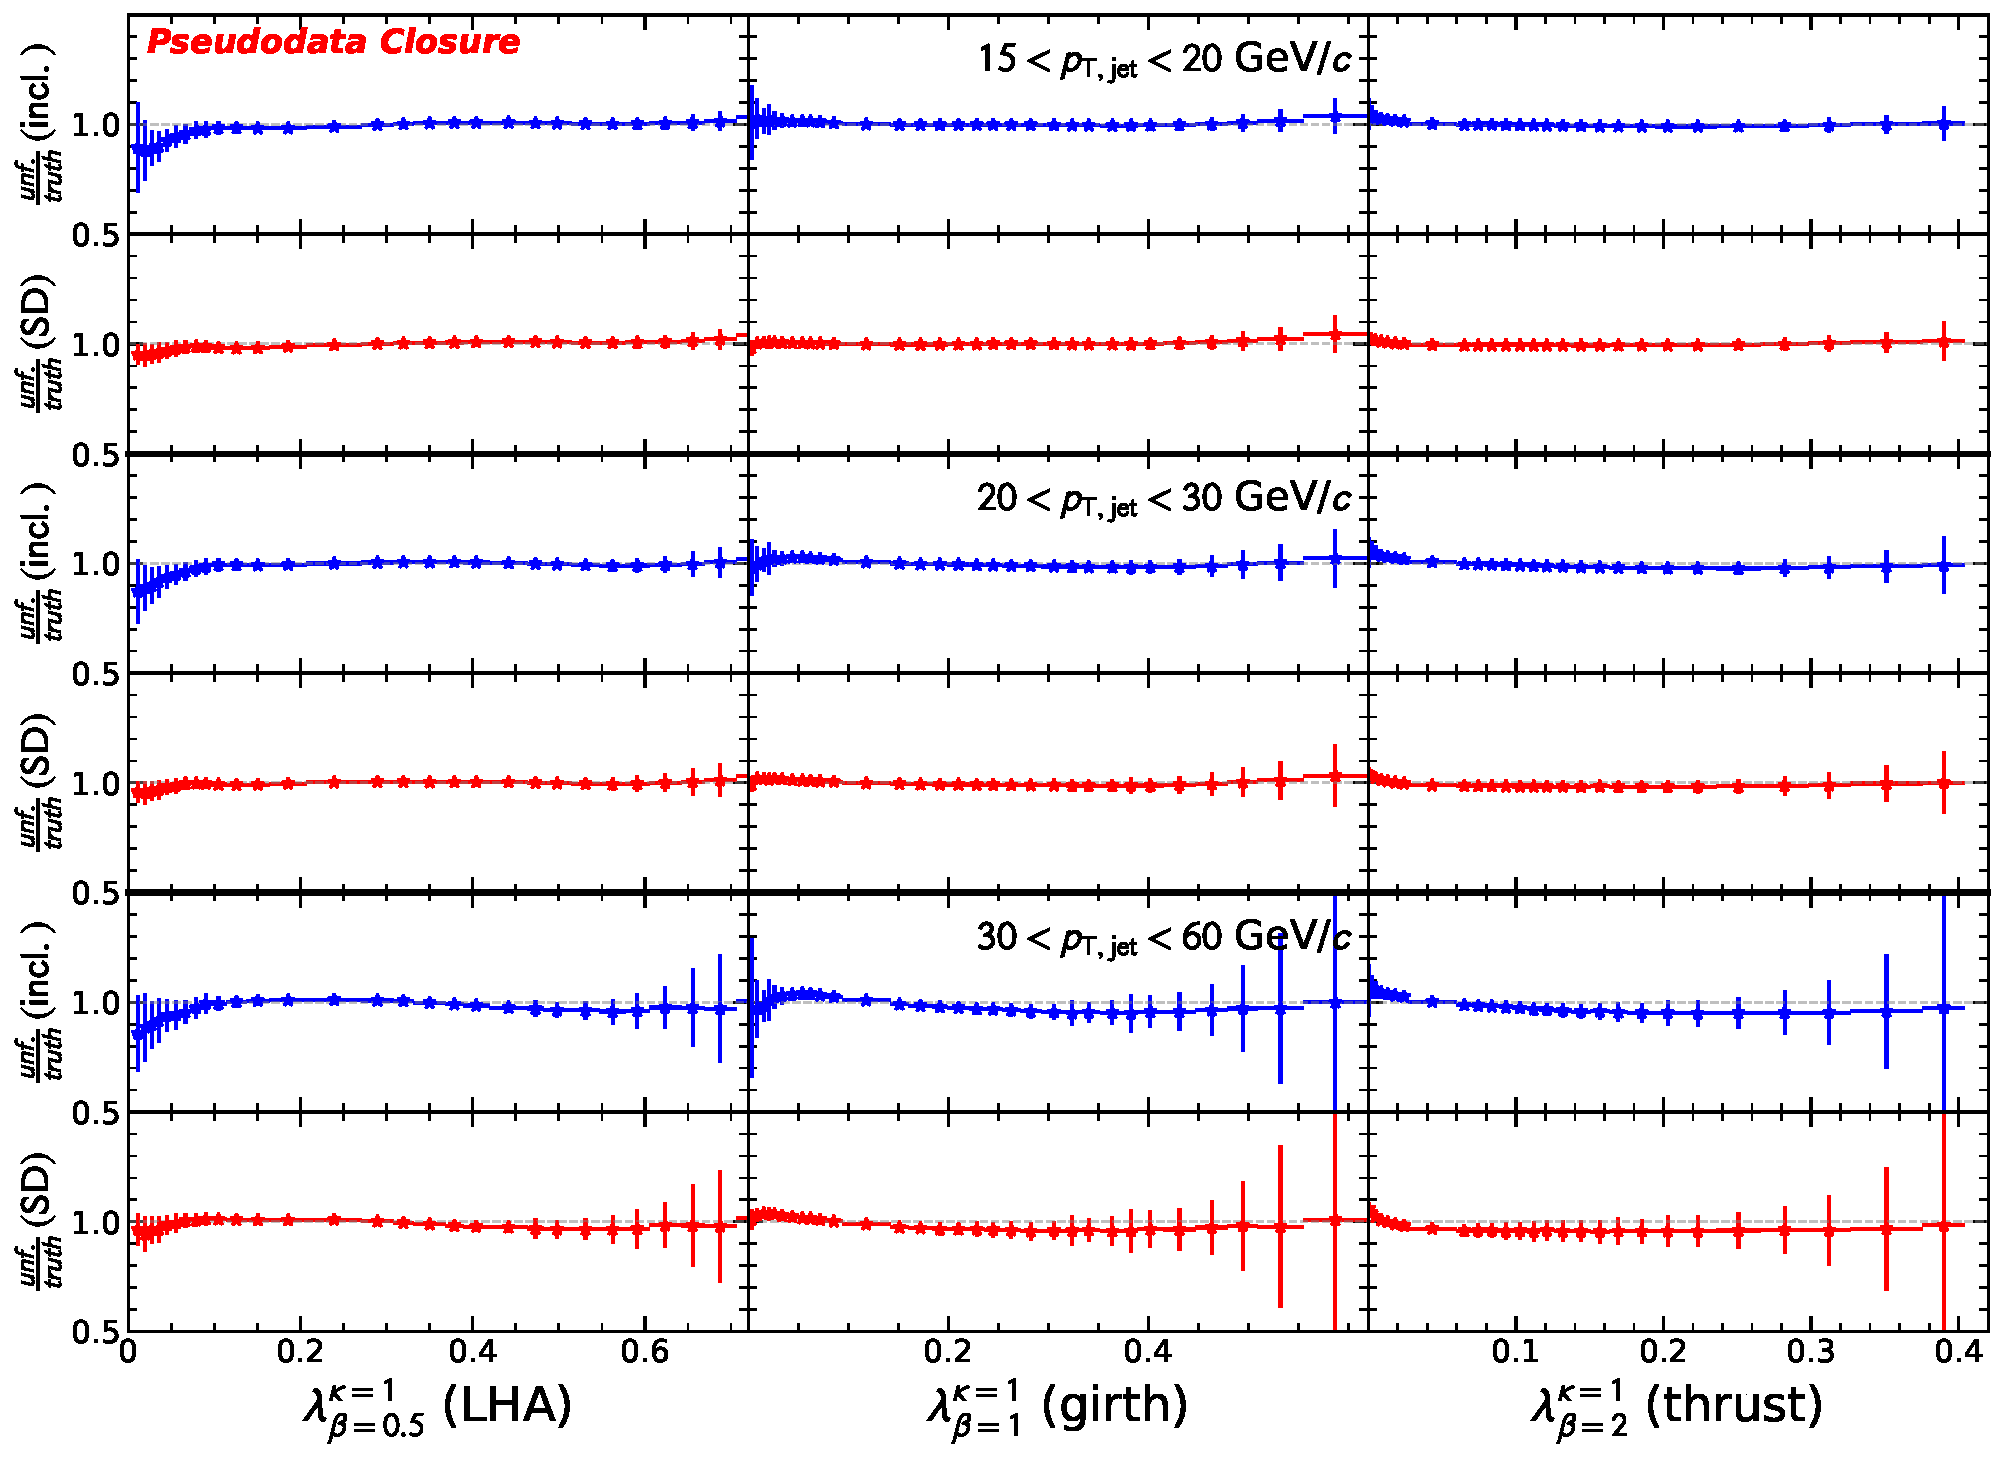
\includegraphics[width=\linewidth,height=0.78\textheight,keepaspectratio]{angularities/pp/fig_dist_ptbins_closure_like.pdf}}%
			\only<2>{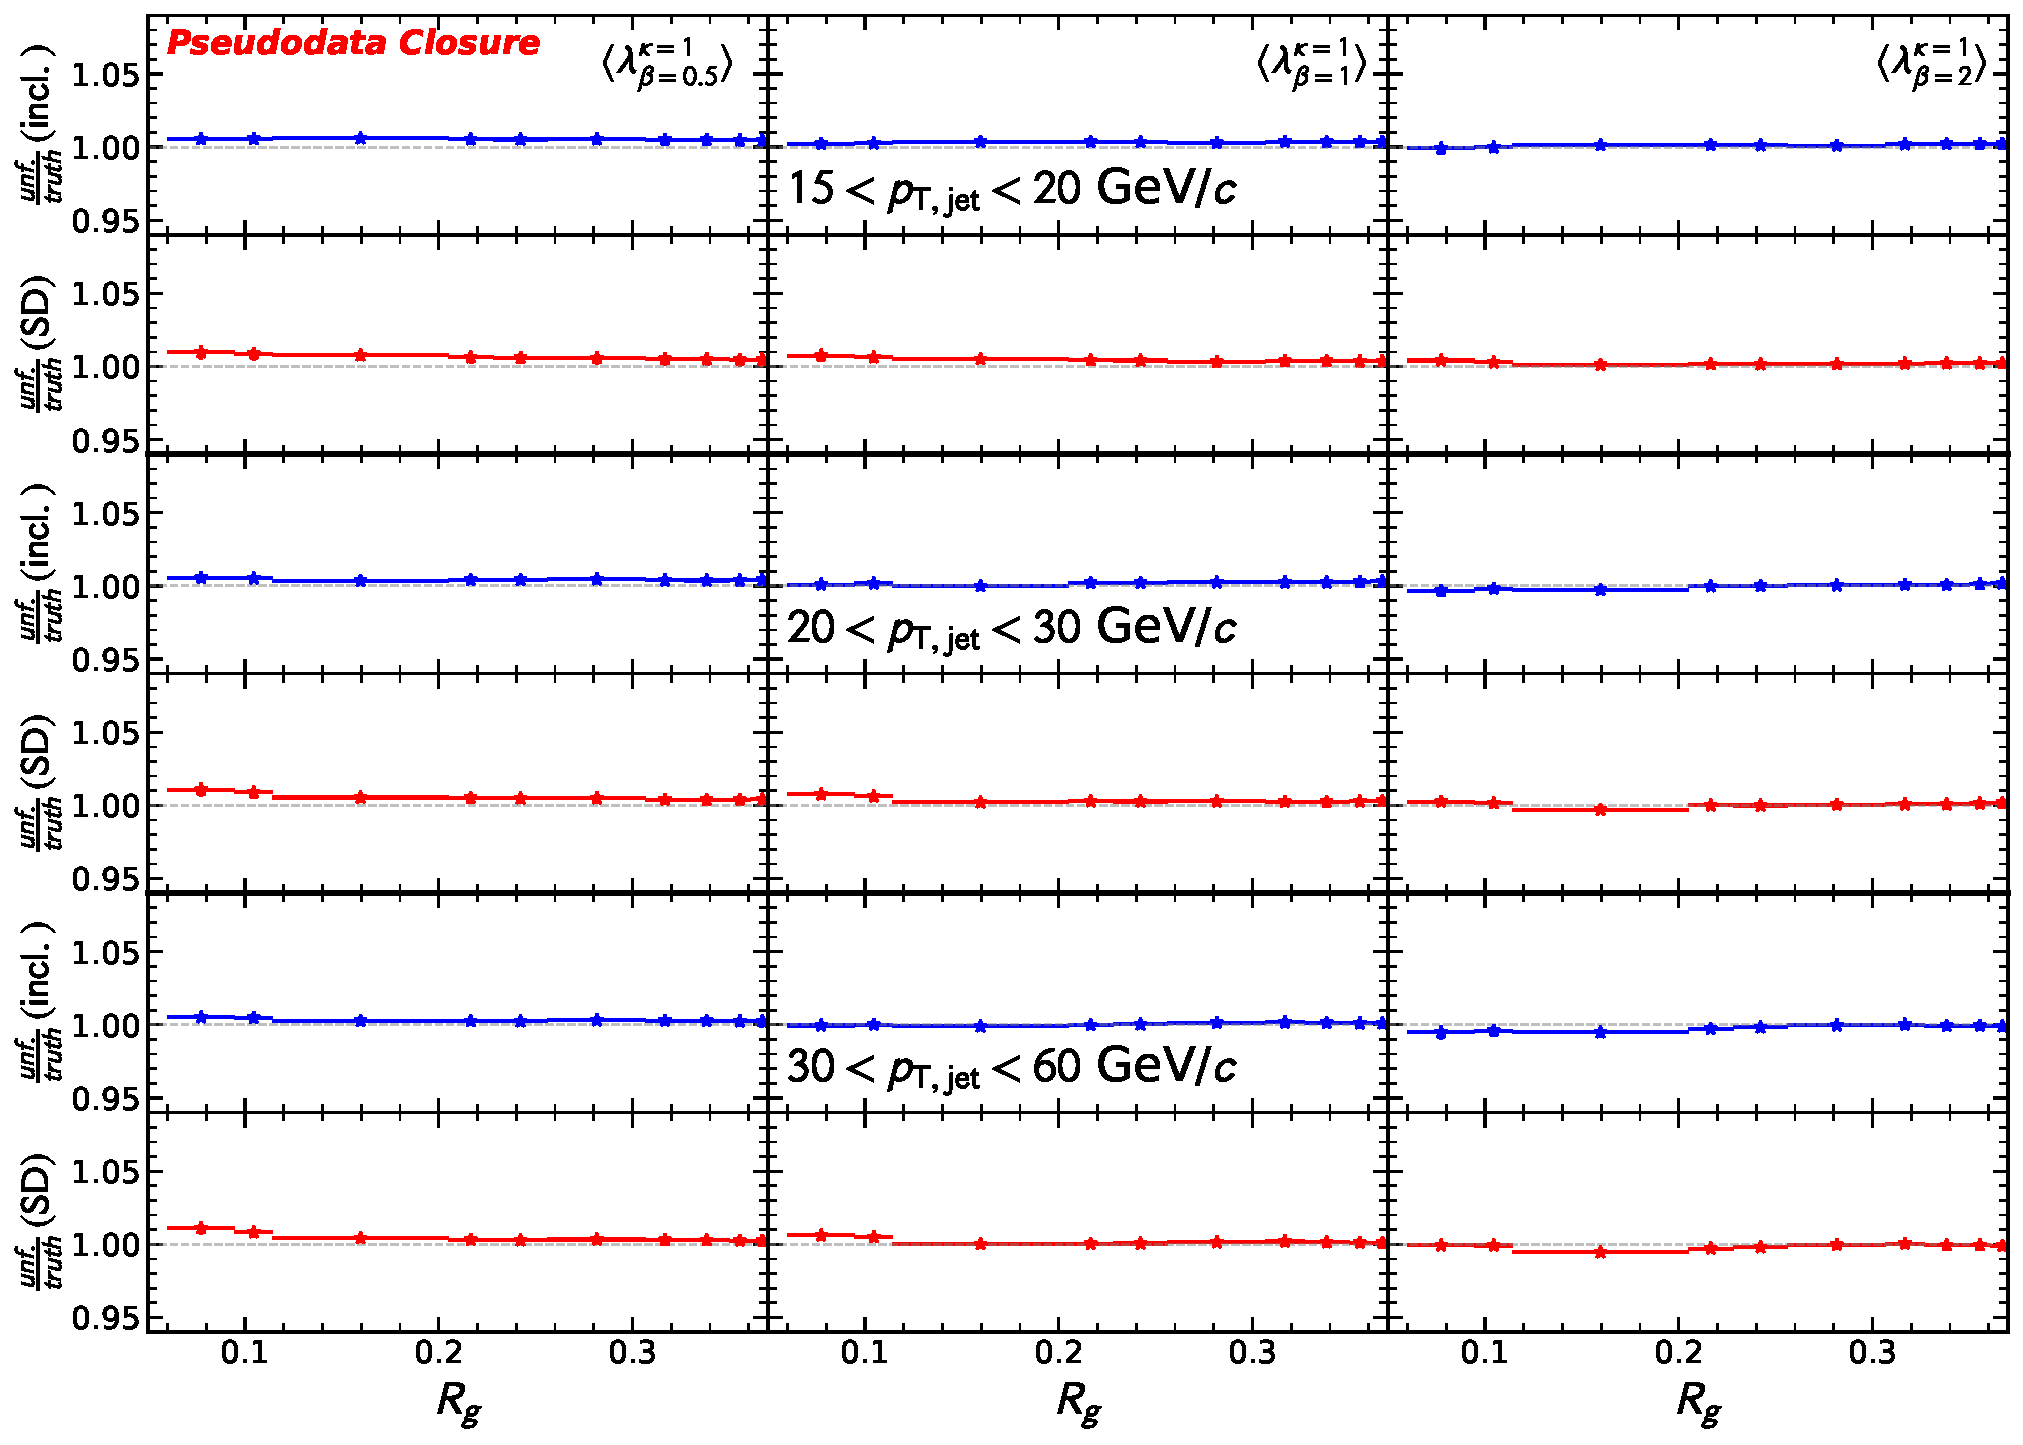
\includegraphics[width=\linewidth,height=0.78\textheight,keepaspectratio]{angularities/pp/fig_dr_ptbins_closure_like.pdf}}
		\end{column}
		\begin{column}{0.39\textwidth}
			\small
			\begin{itemize}
				\item Pseudo-data: \PYsix reweighted to look like data
				\item Unfolded / truth
				\item<1> Distributions: few \%; \(\lesssim\)20\% in tails
				\item<2> Profiles: \textbf{\(\lesssim\)1\%}
			\end{itemize}
		\end{column}
	\end{columns}
\end{frame}

\begin{frame}{Systematic uncertainties}
	\small
	\begin{columns}[T]
		\begin{column}{0.5\textwidth}
			\textbf{Detector}
			\begin{itemize}
				\item Tracking efficiency: 4\%
				\item Hadronic correction: \(f_\mathrm{had} = 1 \to 0.5\)
				\item Tower gain: \(+3.8\%\)
				\item JER: shifted \(p_\mathrm{T}\) bins
			\end{itemize}
			Barlow: drop shifts within stat.\ noise
		\end{column}
		\begin{column}{0.48\textwidth}
			\textbf{Unfolding} (max envelope)
			\begin{itemize}
				\item Iterations: 2 \(\to\) 1, 3
				\item Prior: \PYsix \(\to\) \HWseven, \PYeight
				\item Non-closure
			\end{itemize}
			Total = envelope \(\oplus\) detector
		\end{column}
	\end{columns}
	\vspace{3mm}
	\onslide<2->{
		\begin{block}{Size}
			\textbf{Prior} dominates: few \% at peaks, 20--35\% in tails; profiles 3--6\%; detector \(\lesssim\) few \%
		\end{block}}
\end{frame}

\begin{frame}{Uncertainty breakdown (girth)}
	\centering
	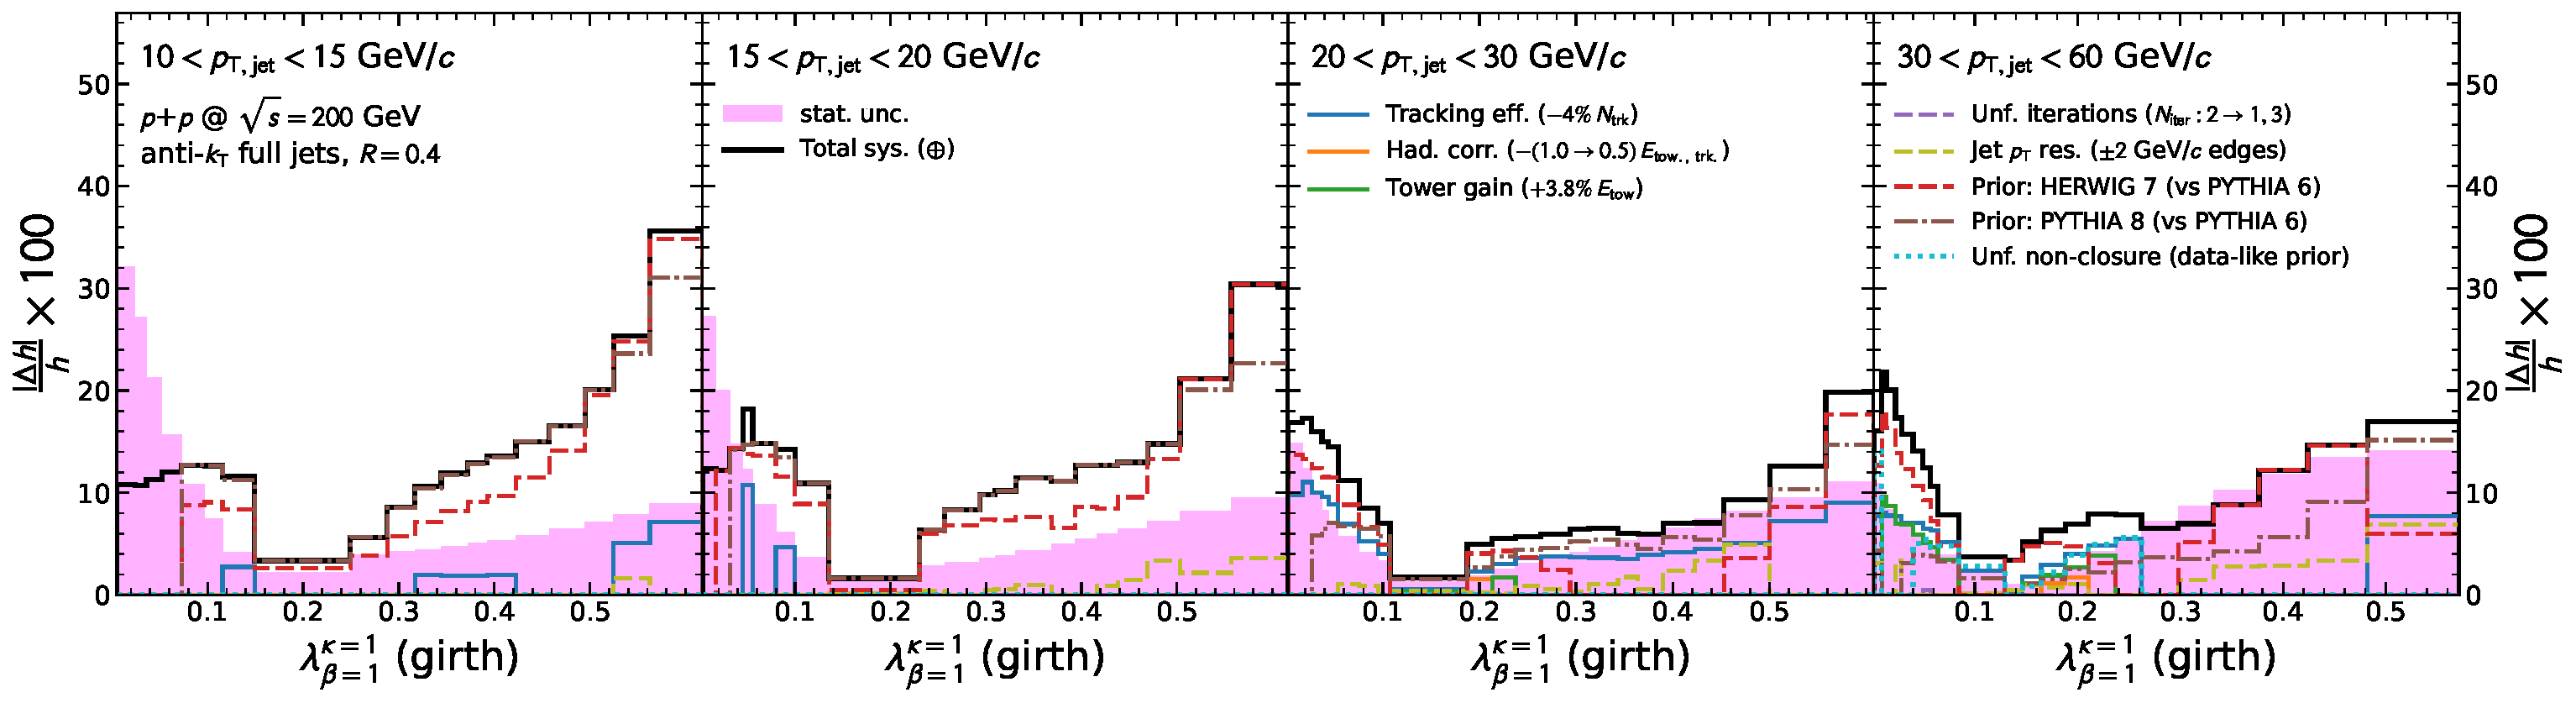
\includegraphics[width=0.9\linewidth]{angularities/pp/sys_ch_ang_k1_b1_hist_ang.pdf}\\
	\onslide<2->{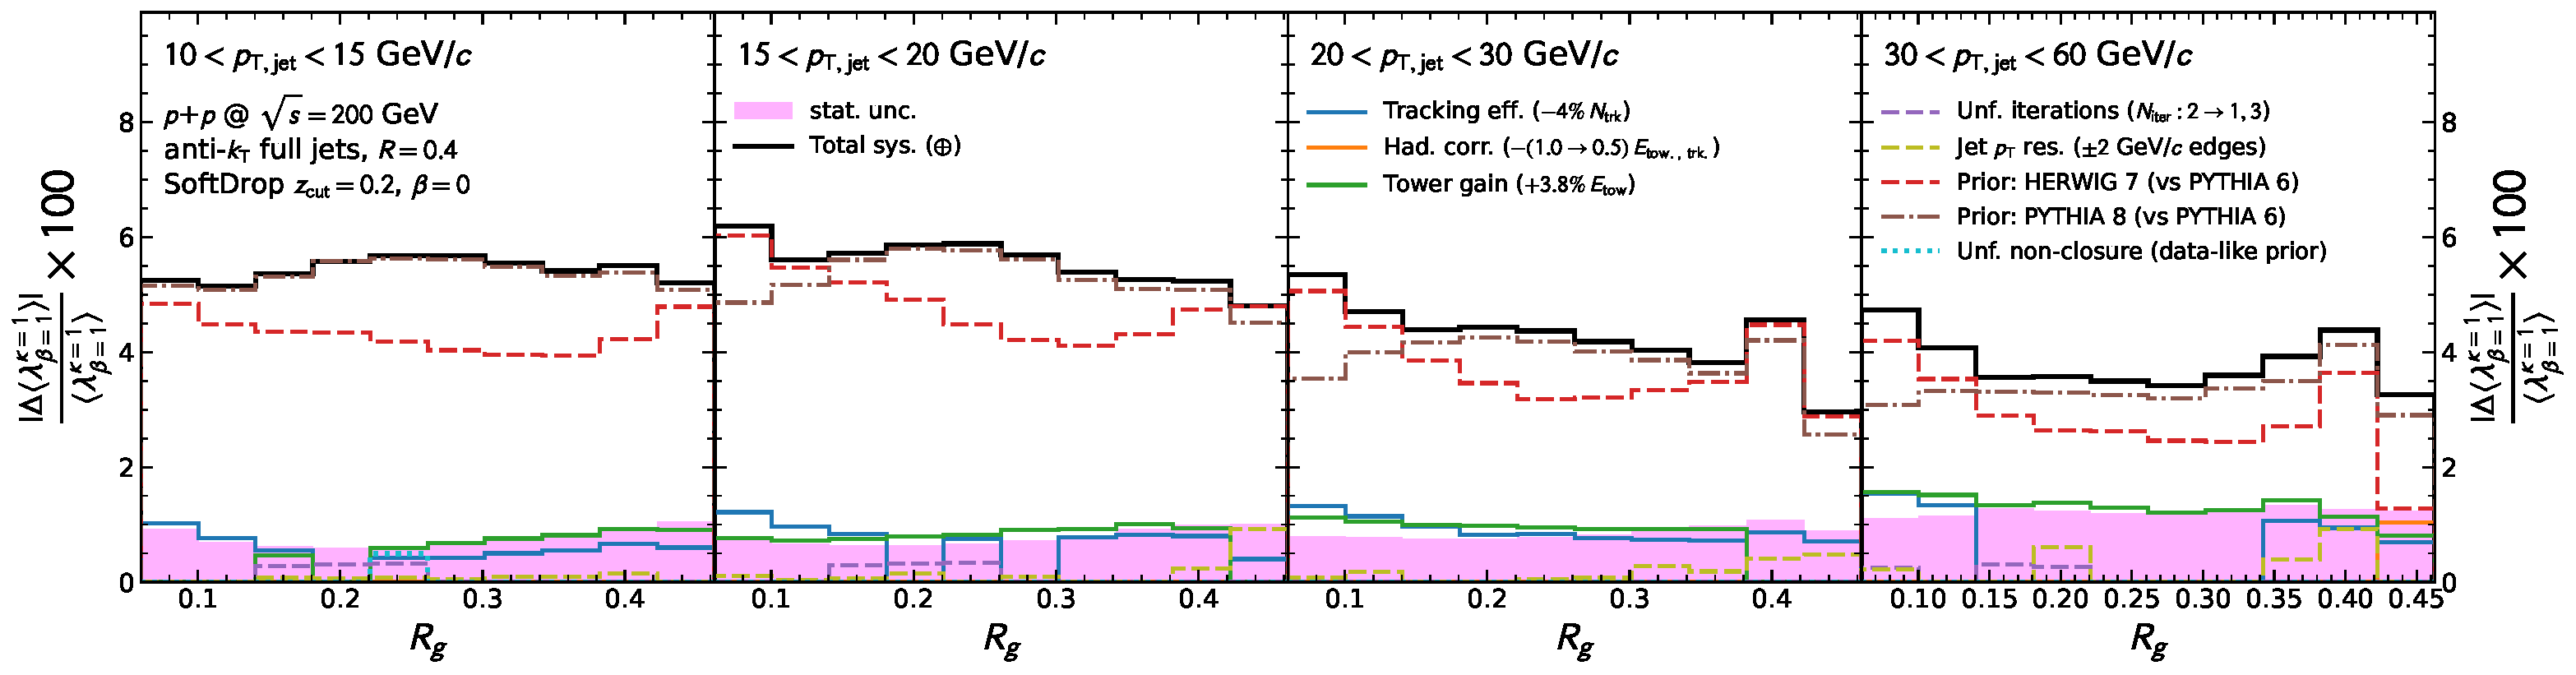
\includegraphics[width=0.9\linewidth]{angularities/pp/sys_ch_ang_k1_b1_prof_incl_vs_sd_dR.pdf}}
\end{frame}

\begin{frame}{Results: inclusive and groomed angularities}
	\centering
	\only<1>{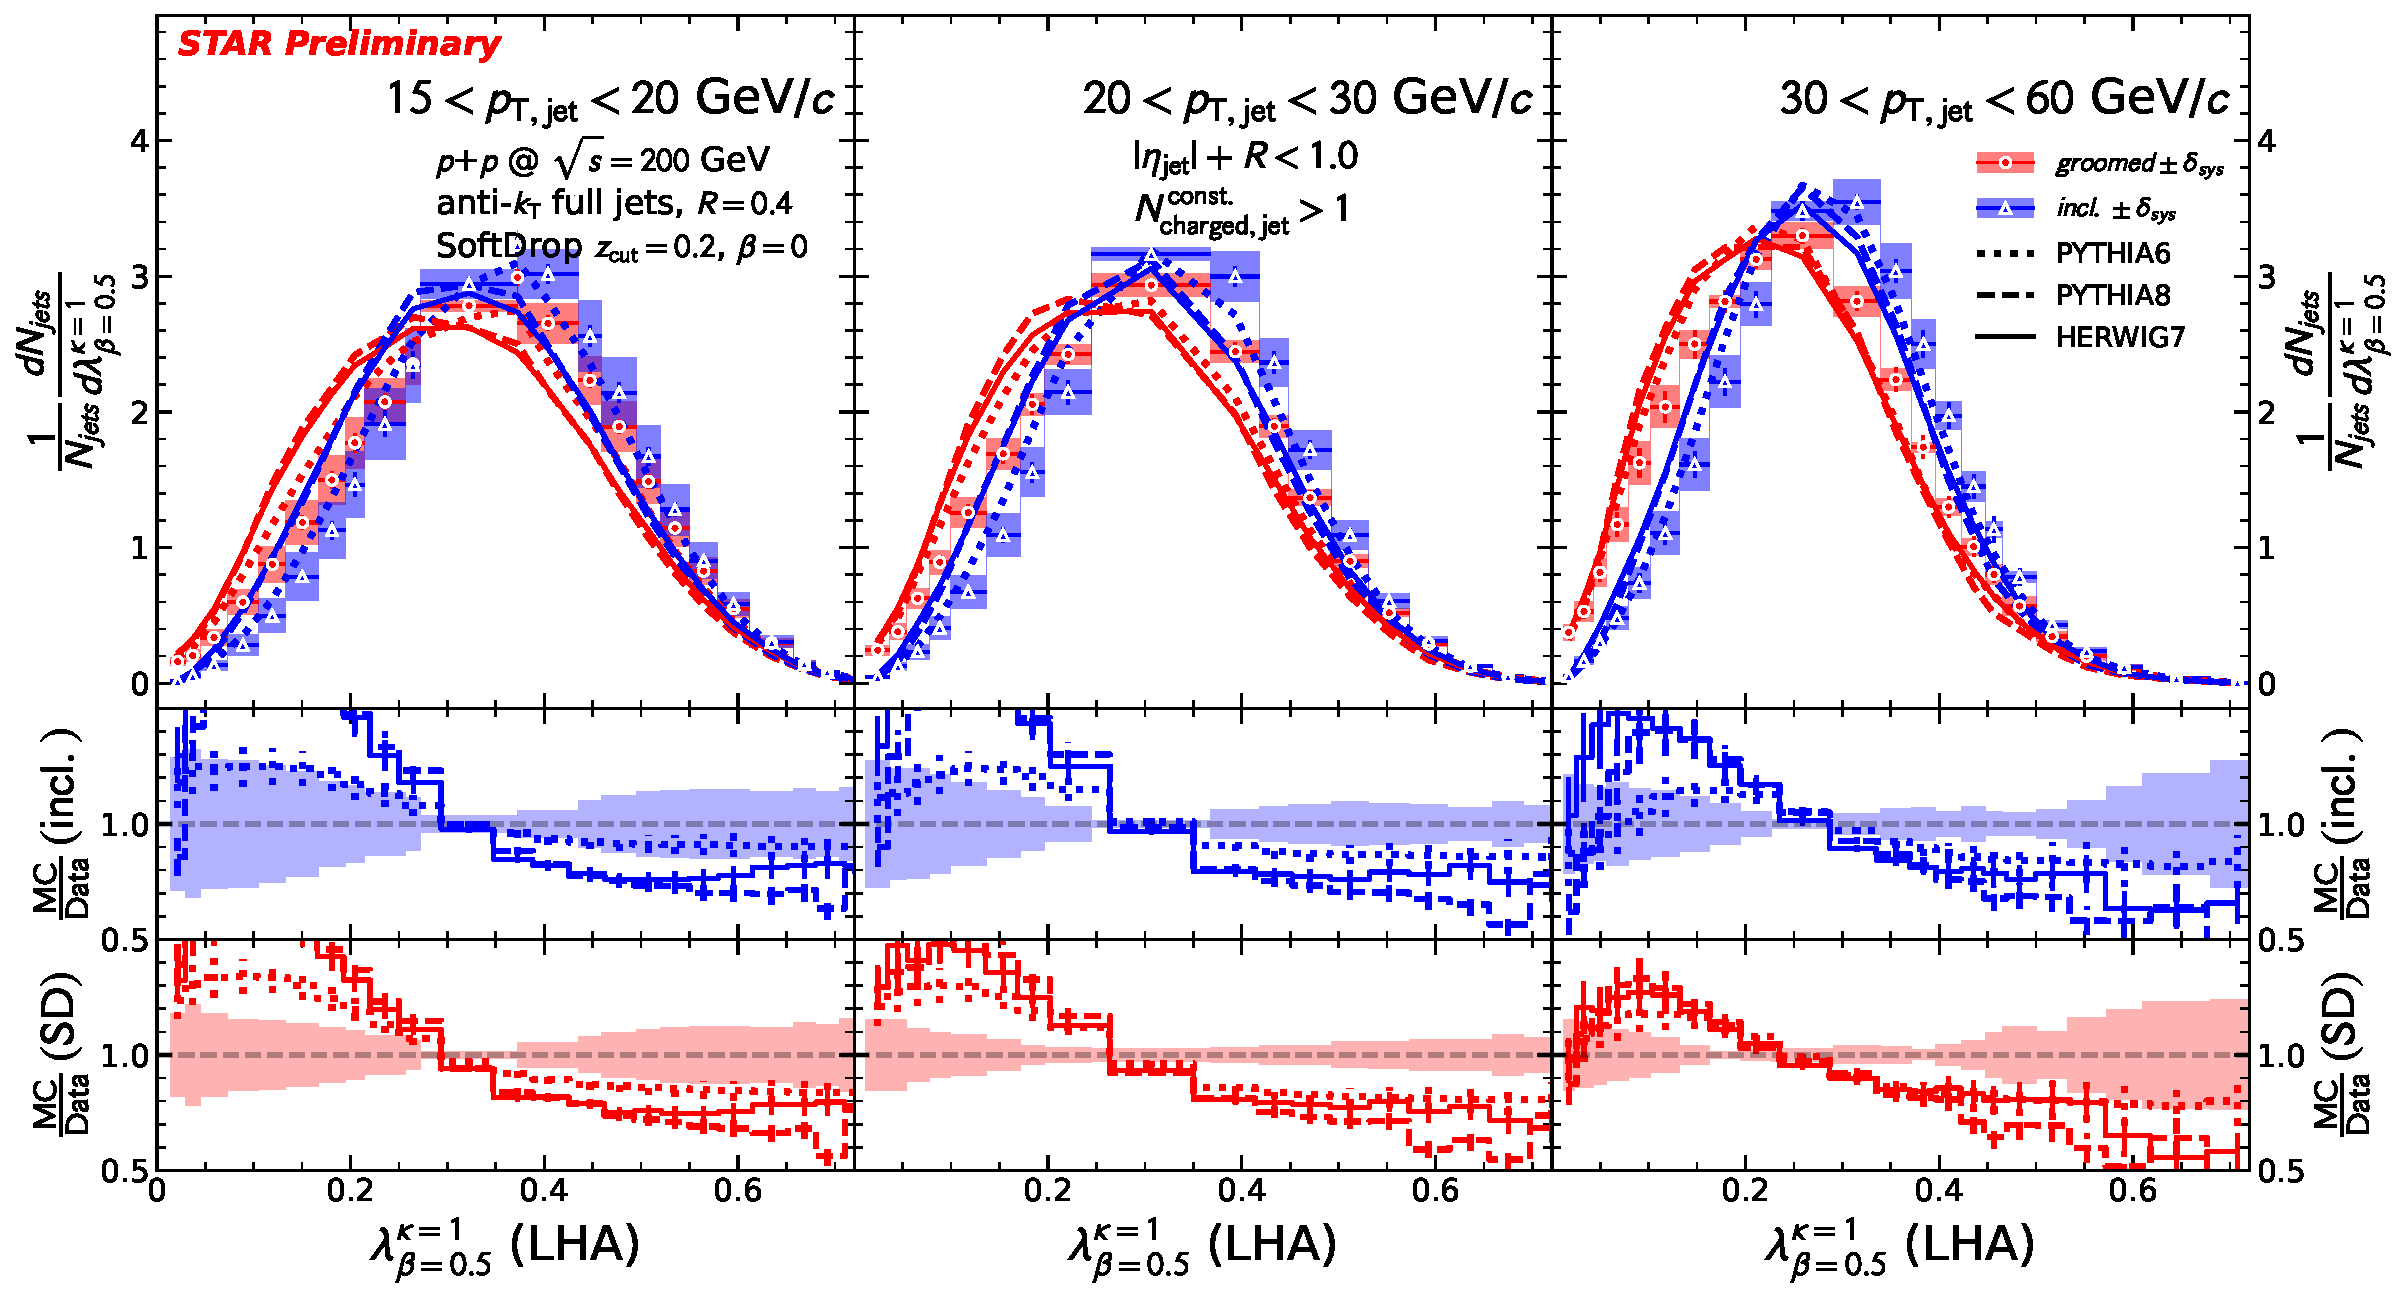
\includegraphics[height=0.7\textheight]{angularities/pp/fig_dist_ptbins_ch_ang_k1_b0_5.pdf}}%
	\only<2>{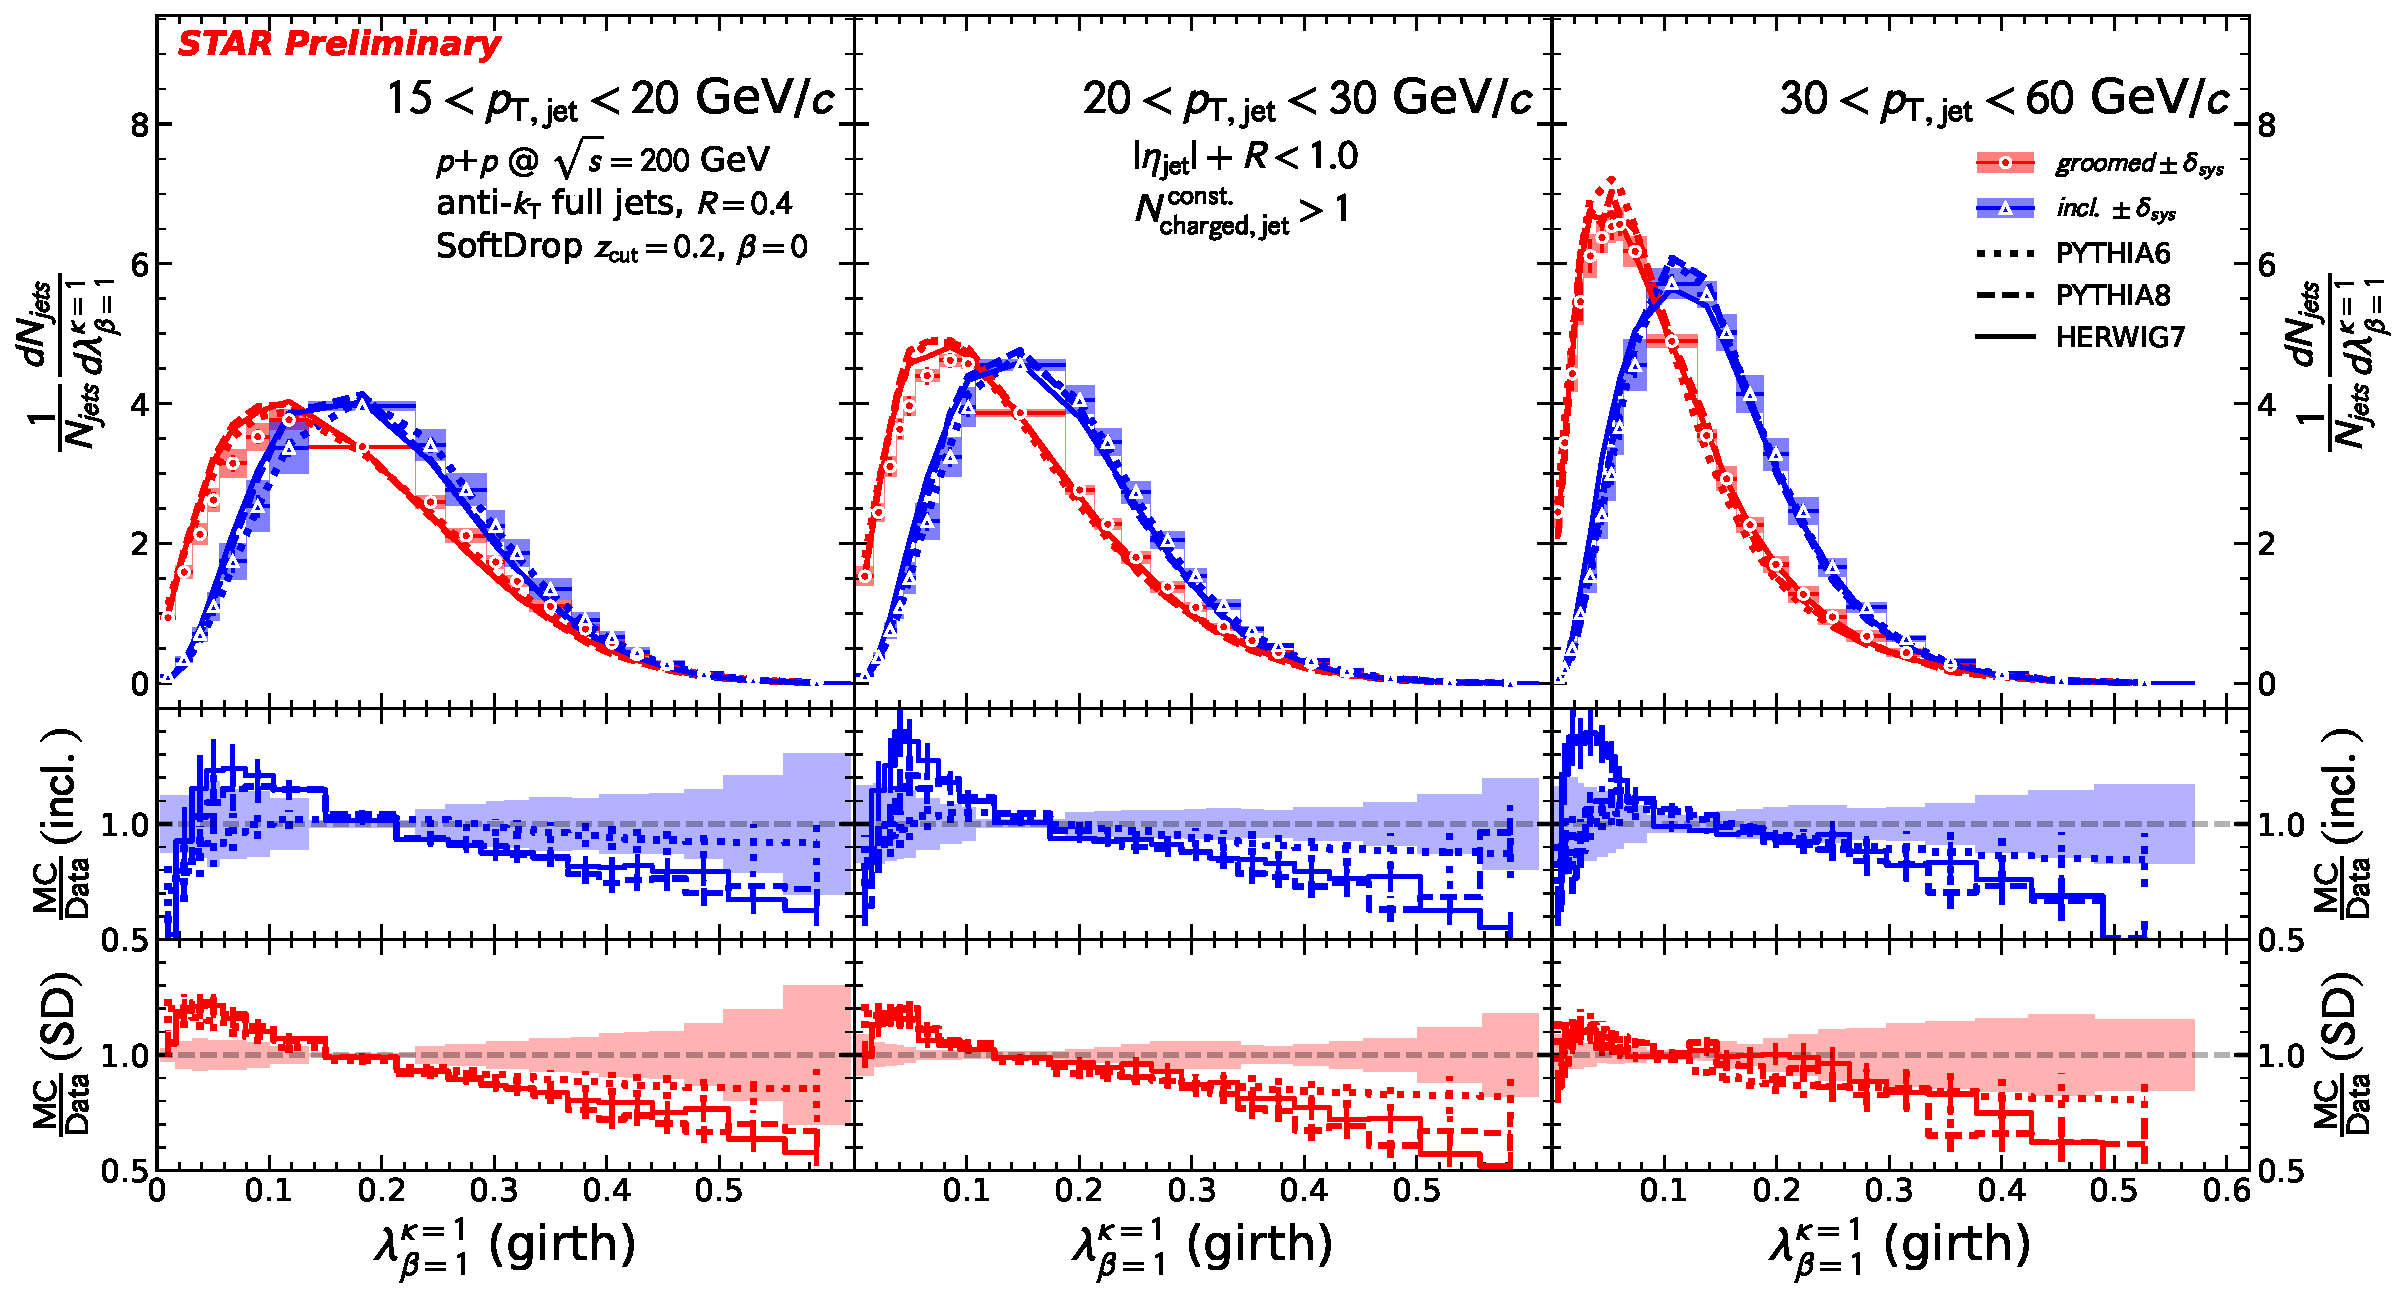
\includegraphics[height=0.7\textheight]{angularities/pp/fig_dist_ptbins_ch_ang_k1_b1.pdf}}%
	\only<3->{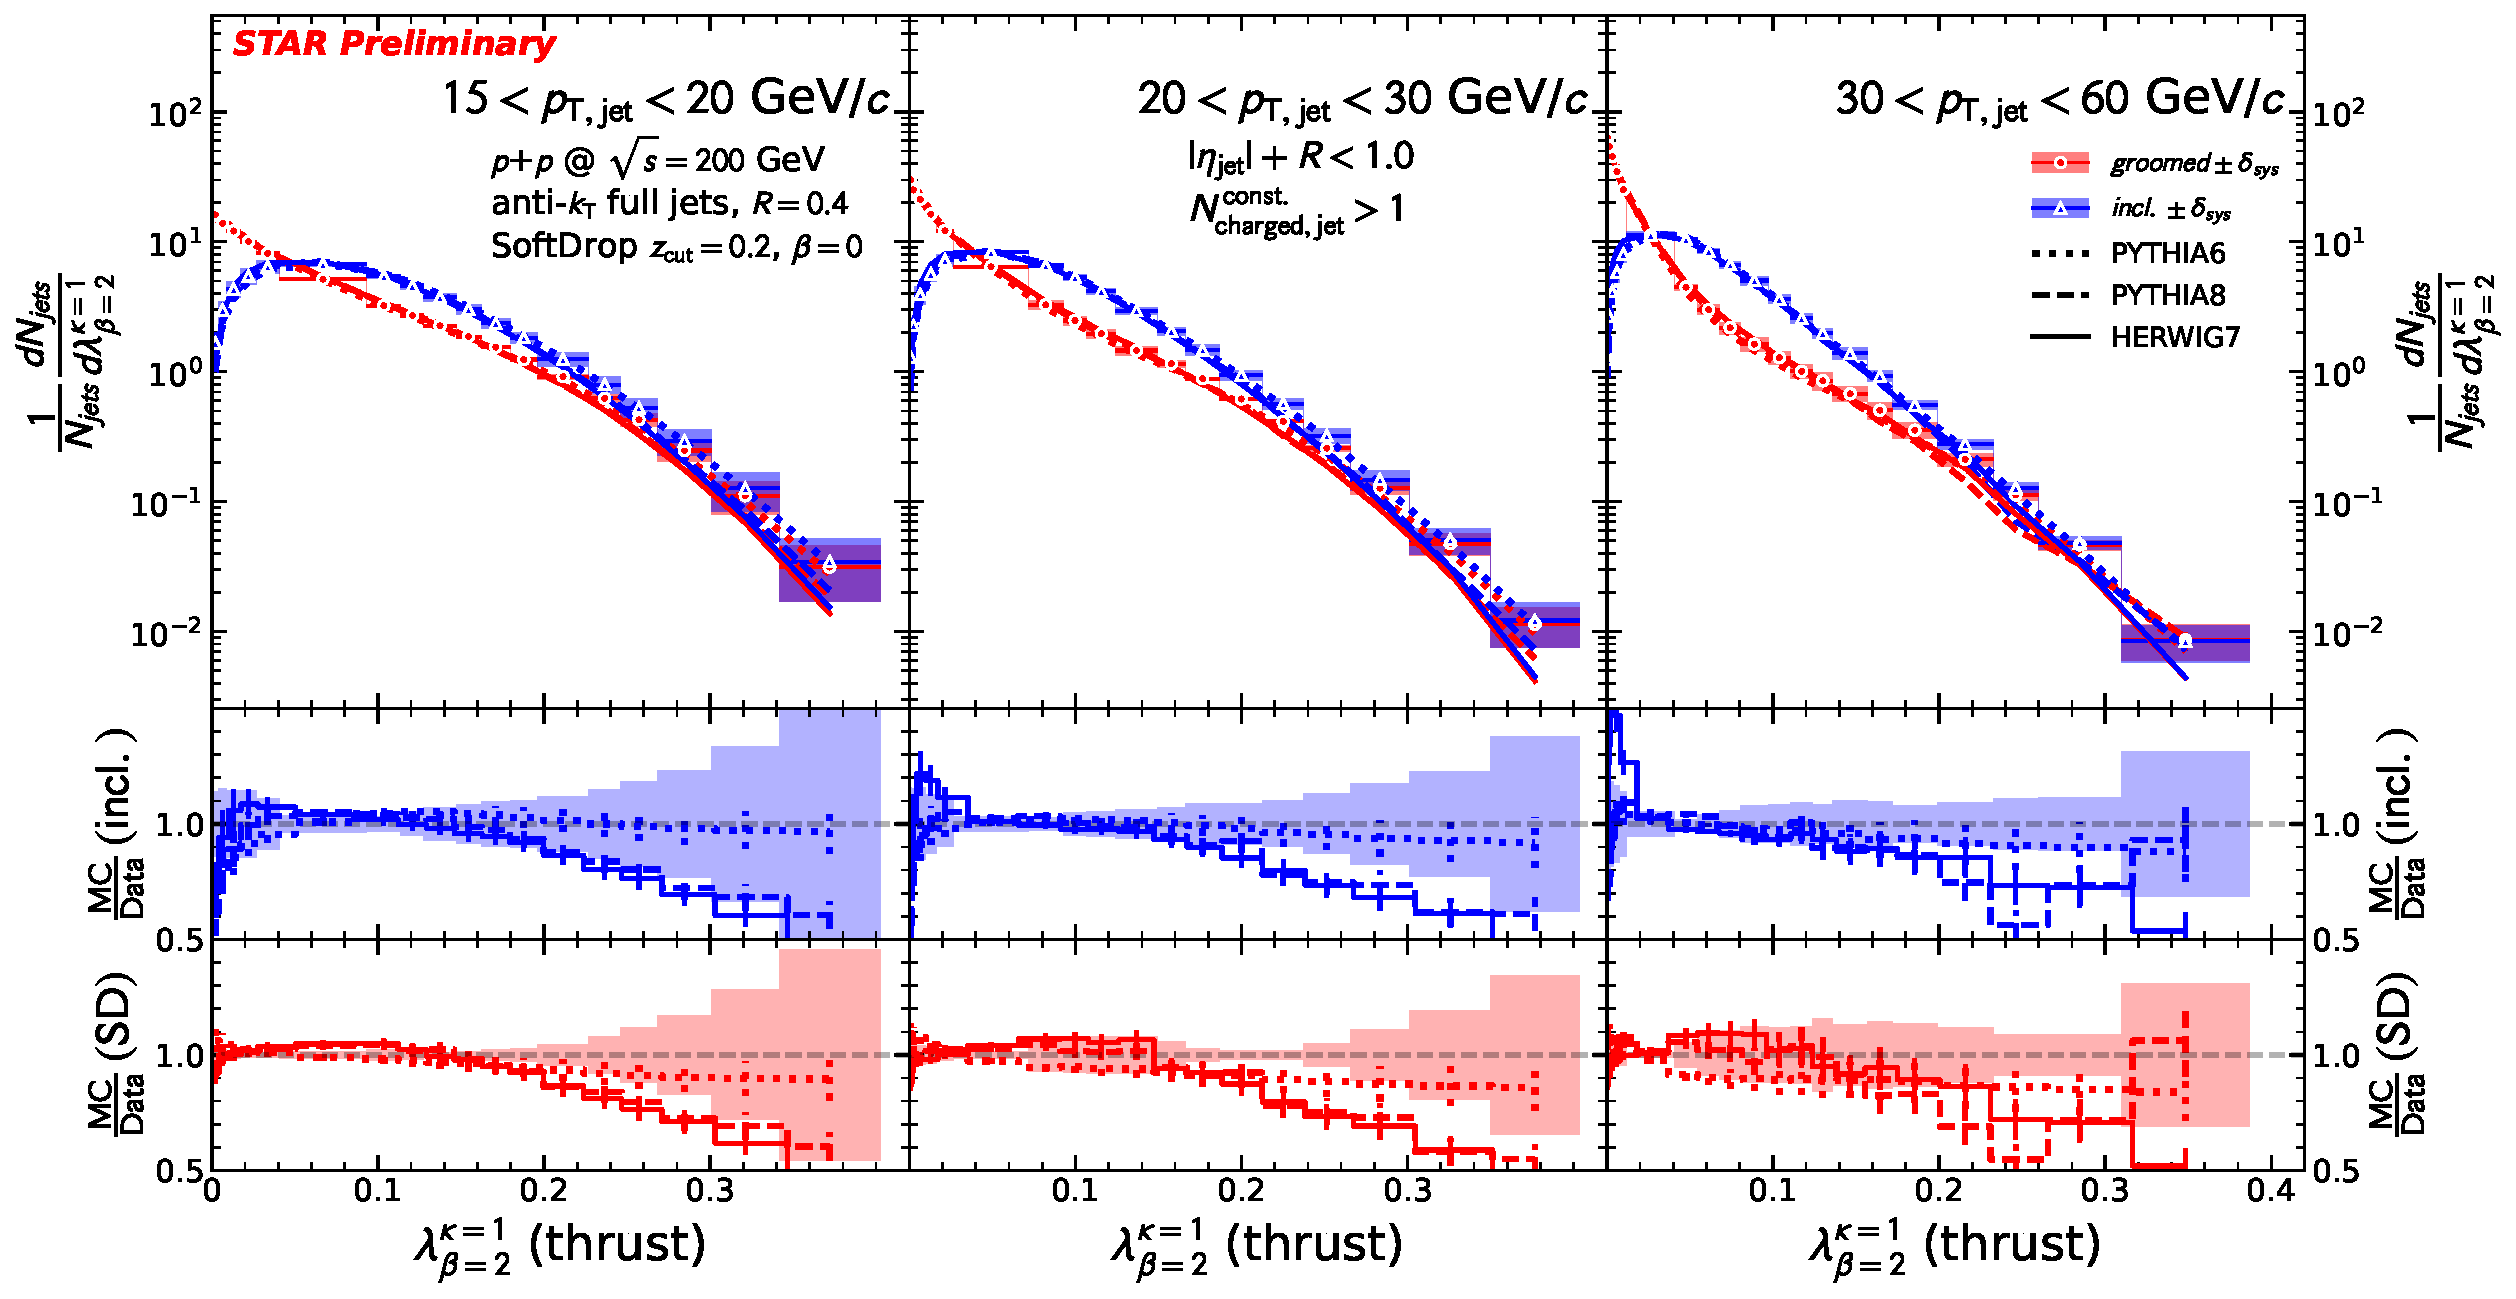
\includegraphics[height=0.7\textheight]{angularities/pp/fig_dist_ptbins_ch_ang_k1_b2.pdf}}
	\begin{itemize}\setlength{\itemsep}{0pt}
		\scriptsize
		\item Jets narrower at high \(p_\mathrm{T}\); grooming \(\to\) smaller \(\lambda\)
		\item<2->  Grooming affects more for larger \(\beta\)
		\item<2-> MC jets \textbf{too narrow}: \HWseven, \PYeight 20--40\% low in tails
		\item<3-> Grooming reduces the gap (\(\beta = 1, 2\))
	\end{itemize}
\end{frame}

\begin{frame}{Results: \(\langle\lambda_\beta\rangle\) vs \Rg}
	\centering
	\only<1>{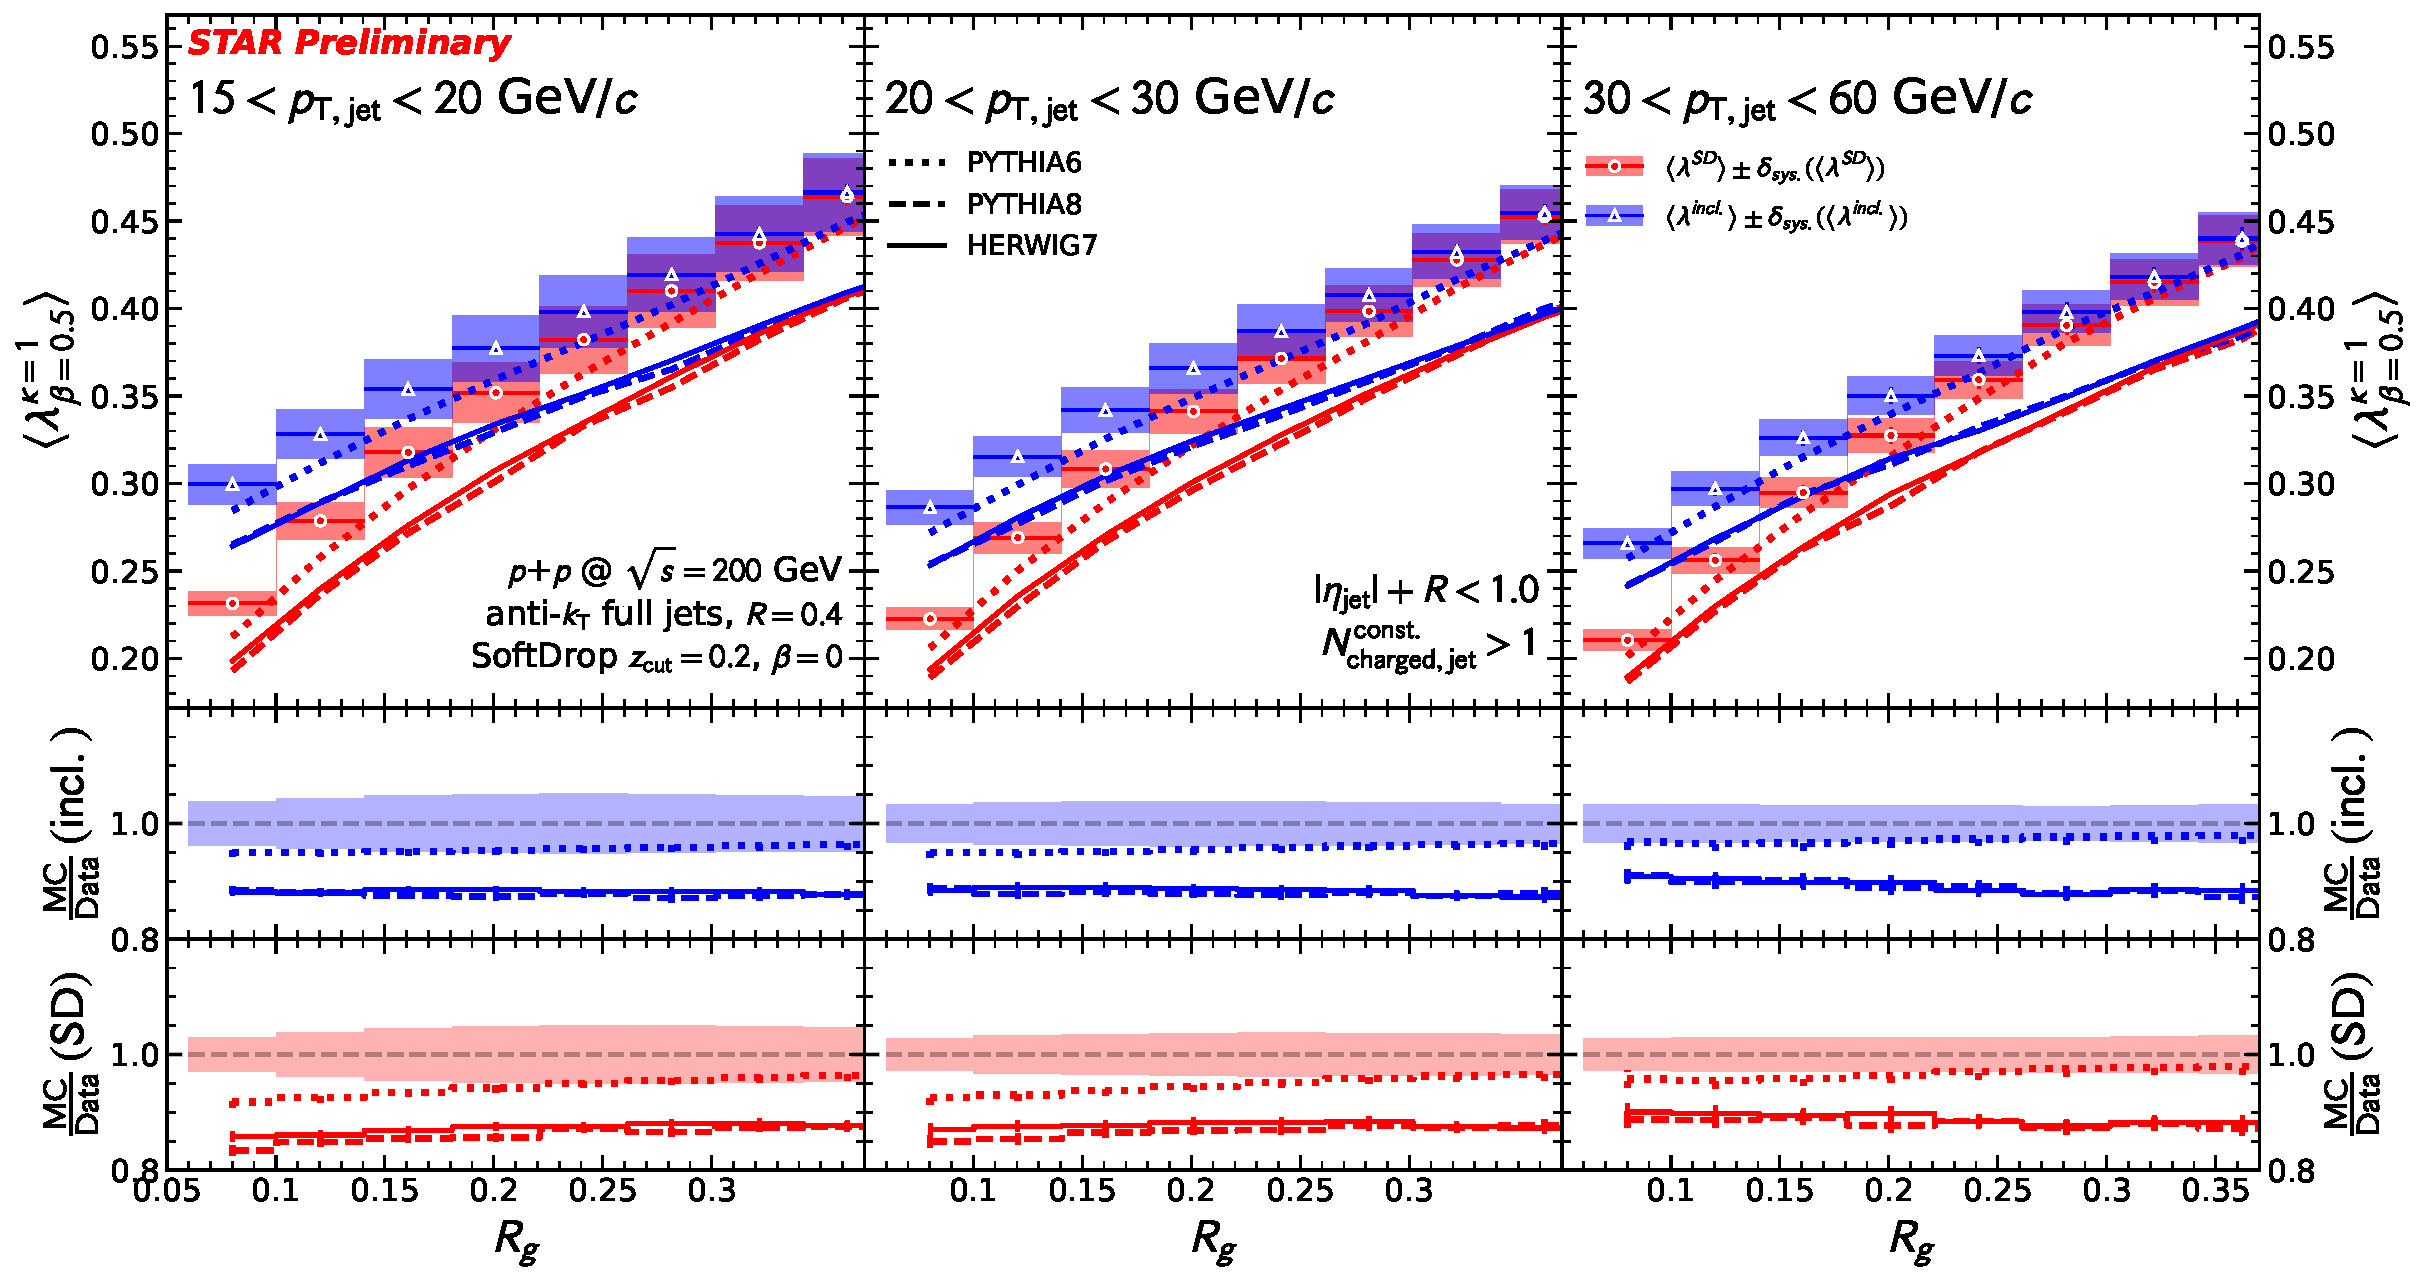
\includegraphics[height=0.7\textheight]{angularities/pp/fig_prof_sd_dR_ptbins_ch_ang_k1_b0_5.pdf}}%
	\only<2>{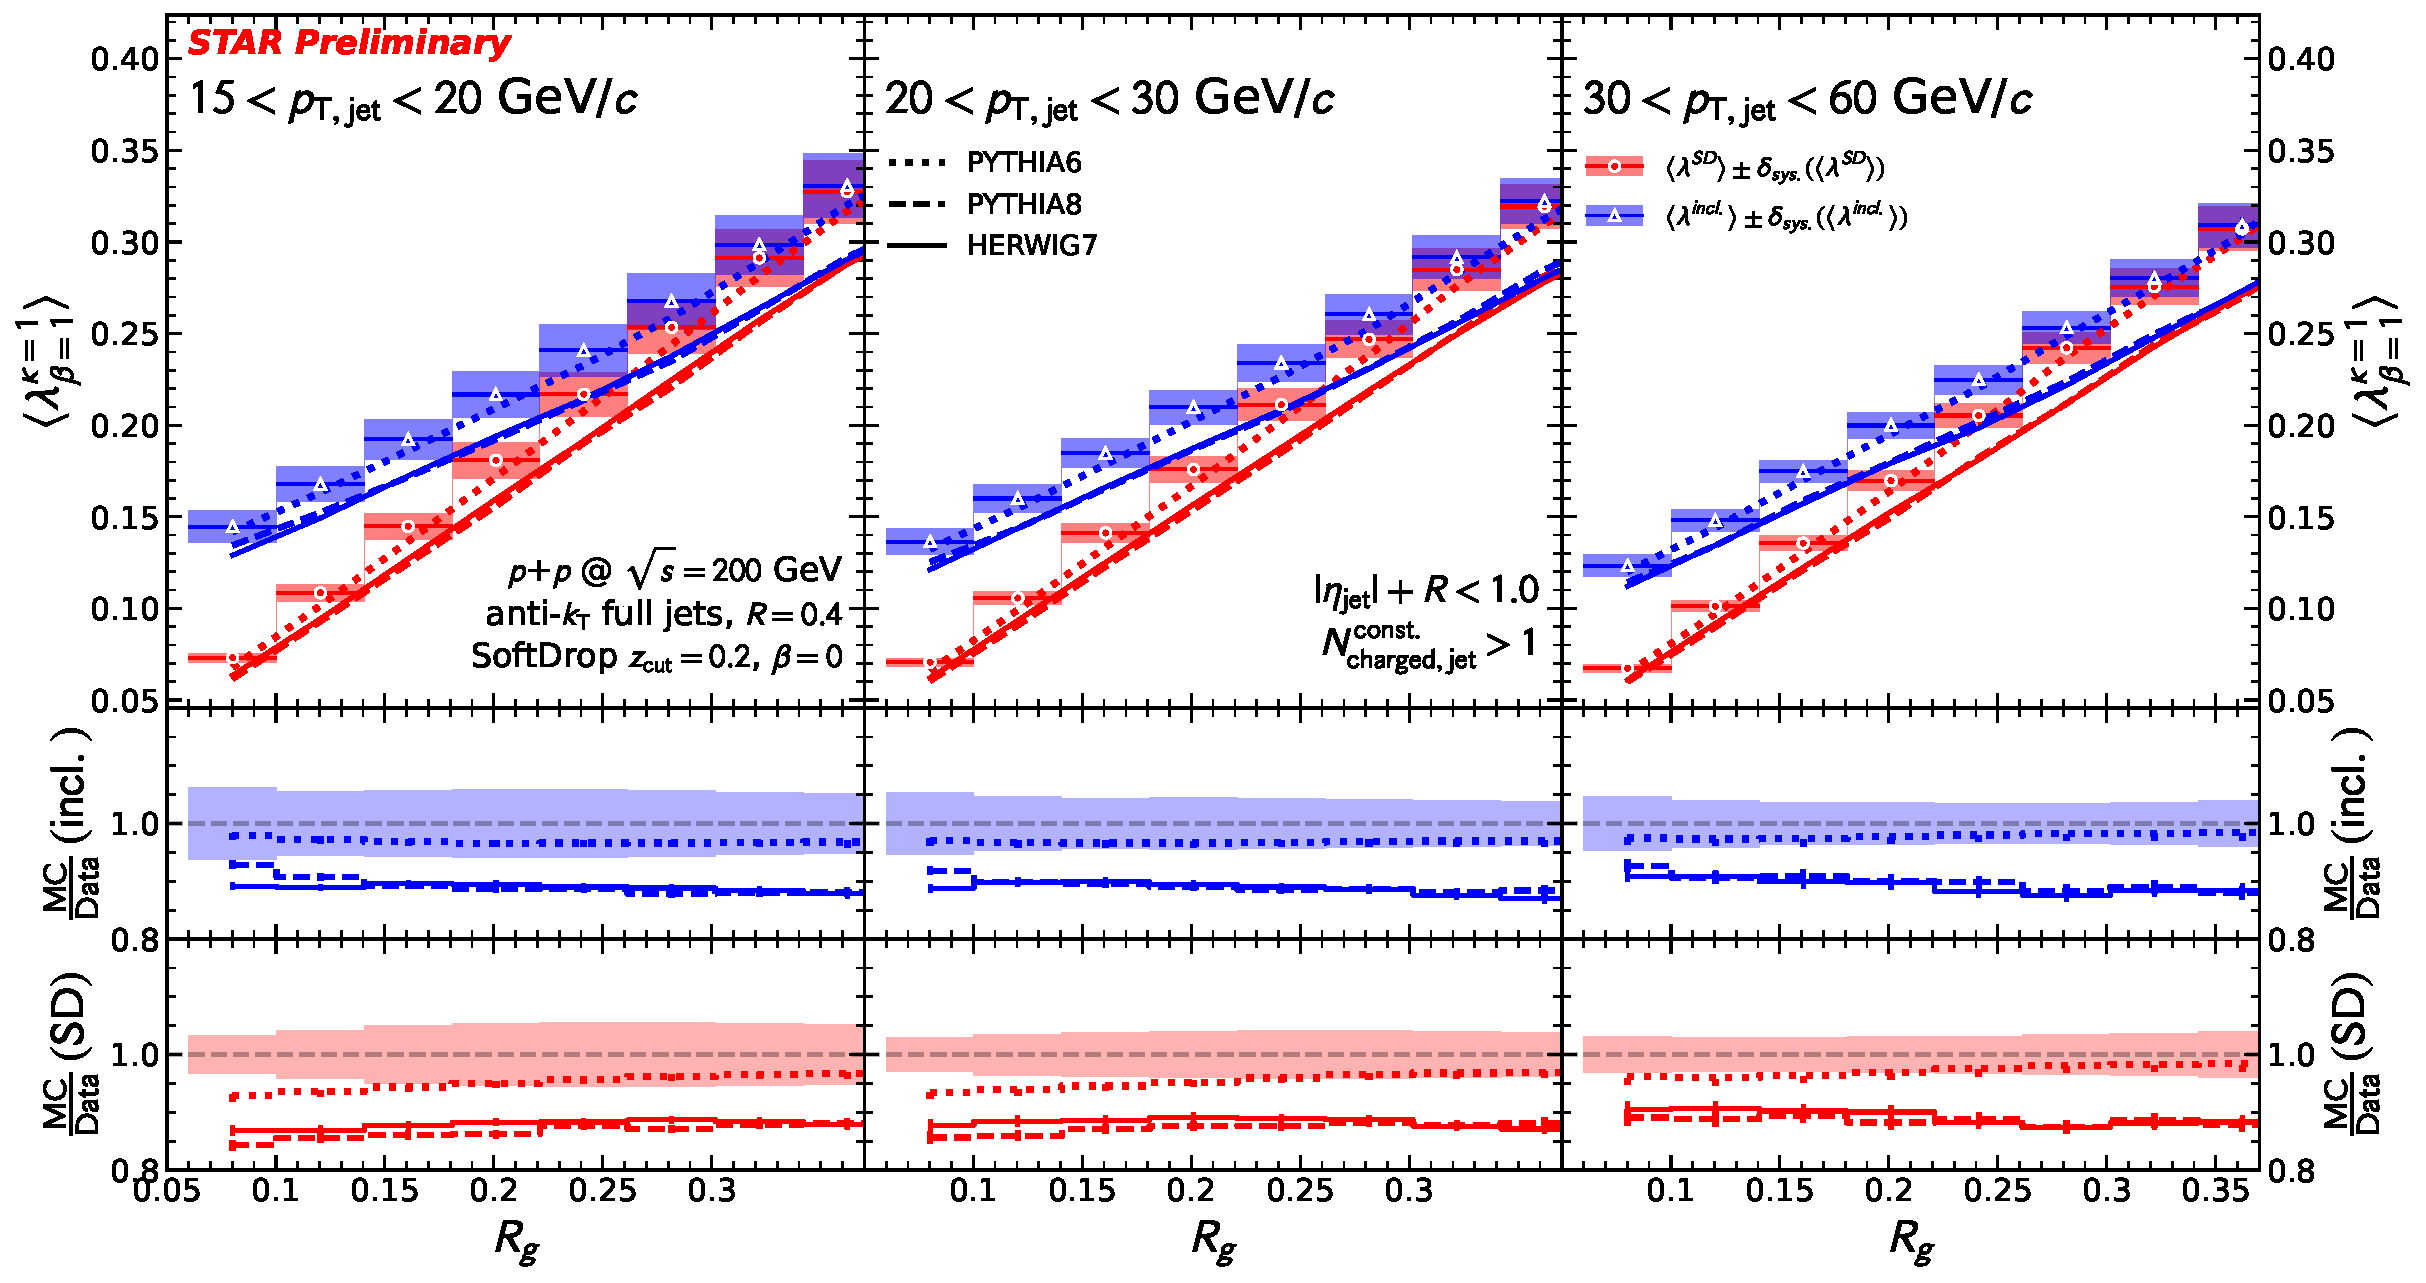
\includegraphics[height=0.7\textheight]{angularities/pp/fig_prof_sd_dR_ptbins_ch_ang_k1_b1.pdf}}%
	\only<3->{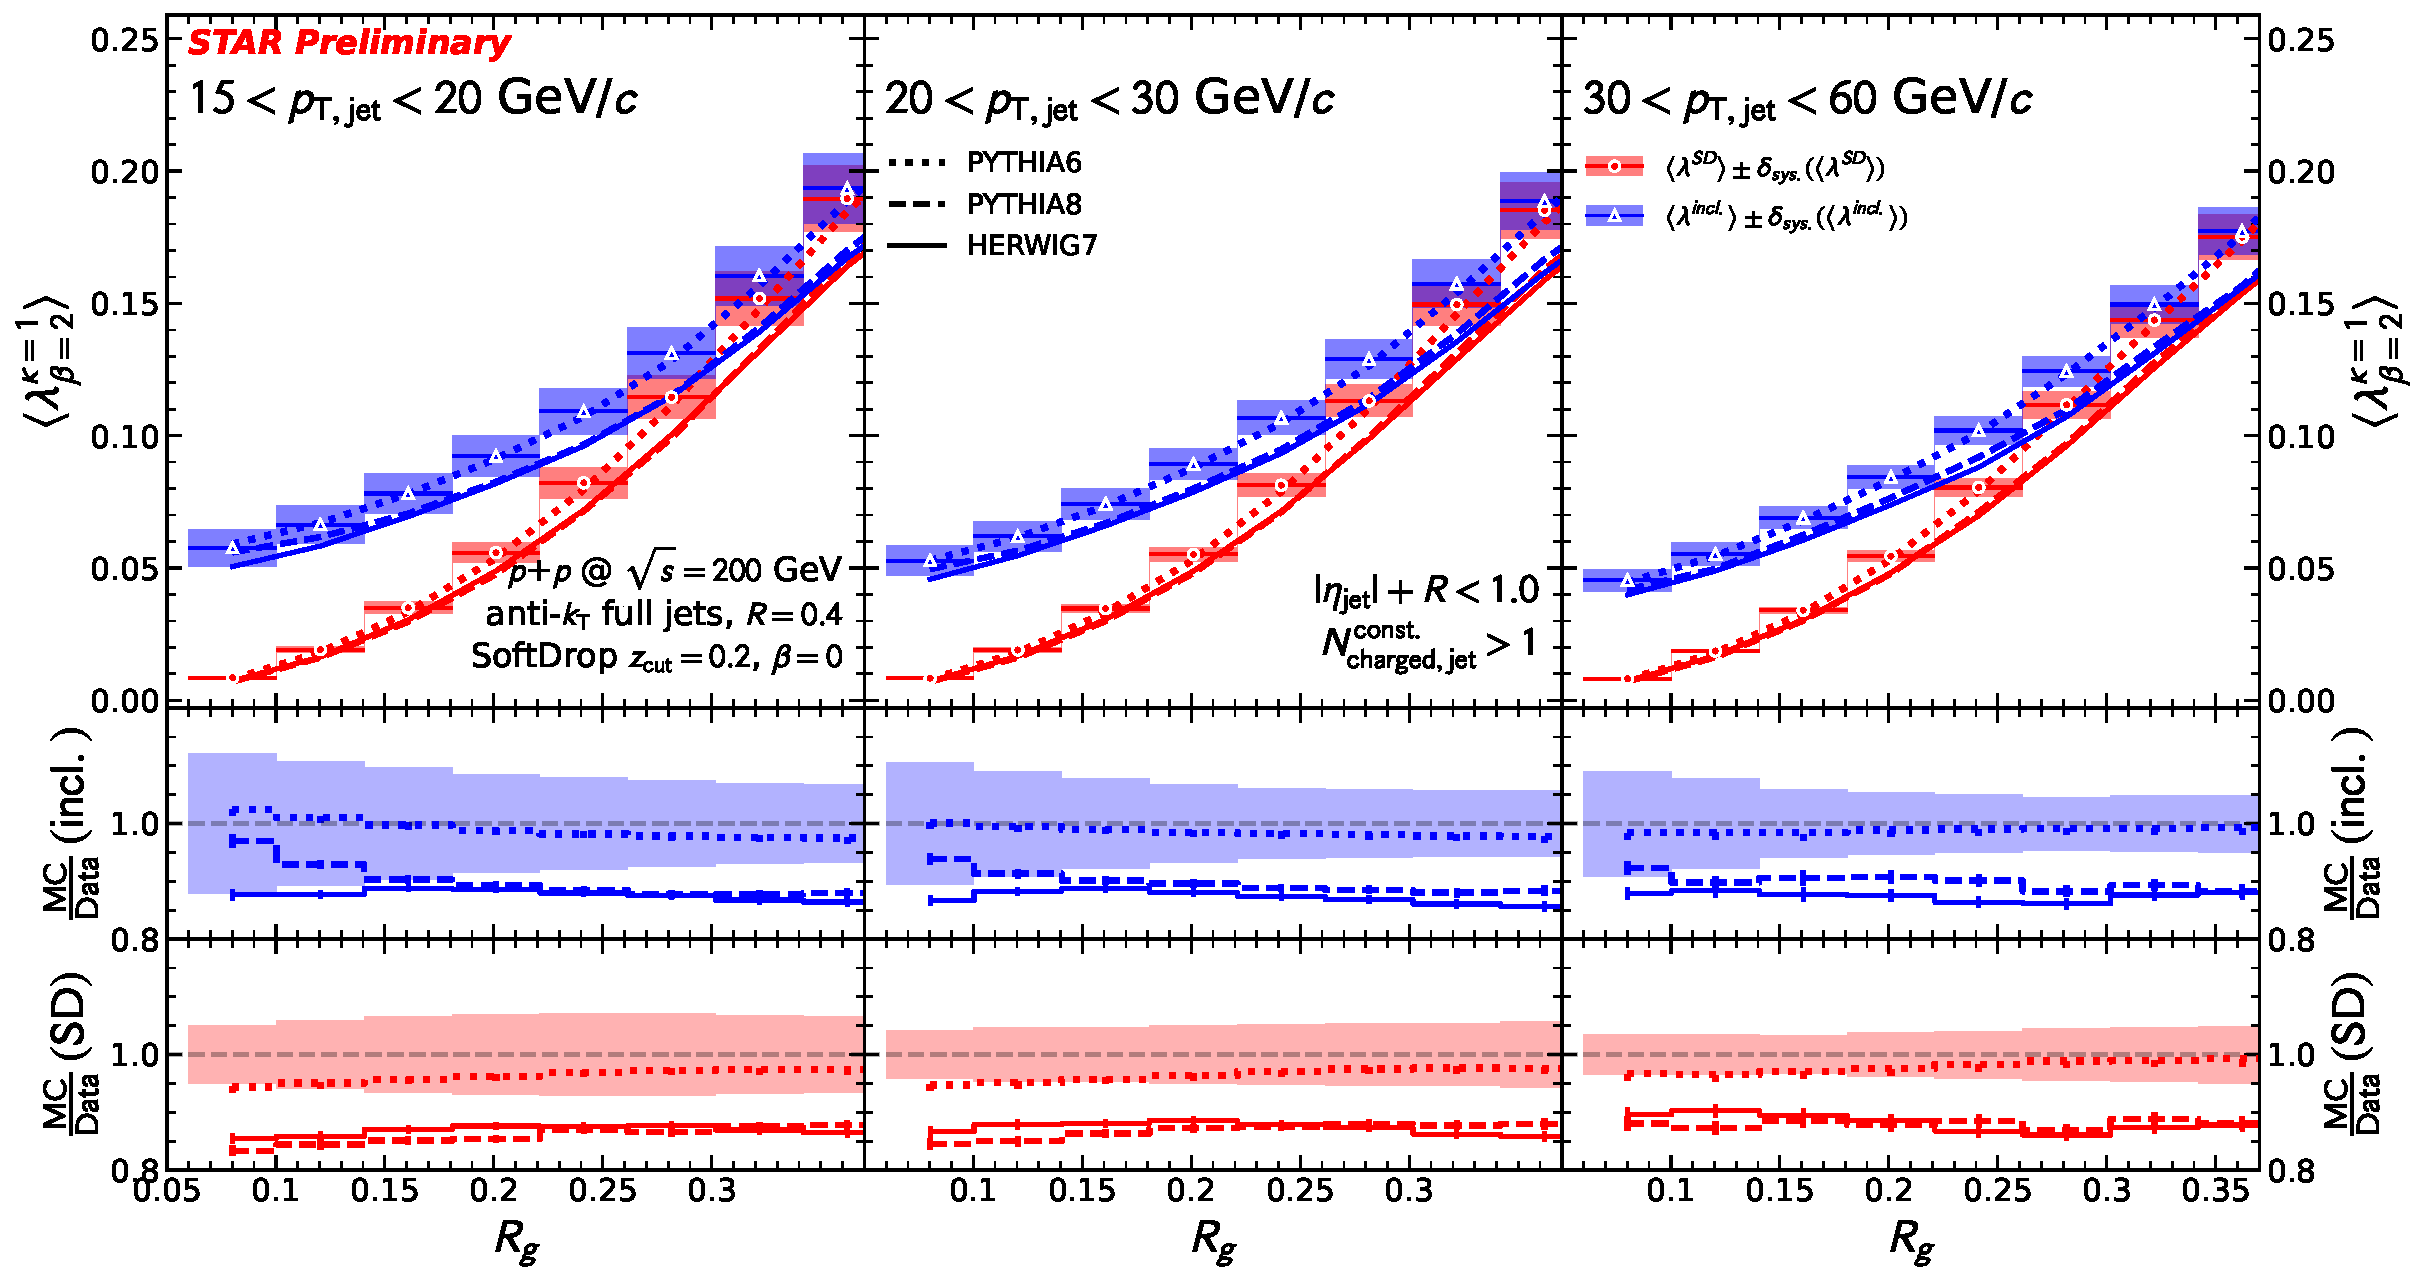
\includegraphics[height=0.7\textheight]{angularities/pp/fig_prof_sd_dR_ptbins_ch_ang_k1_b2.pdf}}
	\begin{itemize}\setlength{\itemsep}{0pt}
		\scriptsize
		\item Rises with \Rg (\(\sim R_\mathrm{g}^\beta\) groomed); incl.\ \(\to\) groomed at large \Rg
		\item<2-> Weak \(p_\mathrm{T}\) dependence at fixed \Rg \(\Rightarrow\) narrowing = \Rg shift
		\item<3-> \HWseven, \PYeight \alert{10--15\% low at every \Rg}
	\end{itemize}
\end{frame}

\begin{frame}{What the profiles add}
	\begin{block}{Distributions}
		\HWseven, \PYeight: jets too narrow
	\end{block}
	\onslide<2->{
		\begin{block}{Profiles vs \Rg}
			Same splitting angle, still too little radiation \\
			\(\Rightarrow\) \alert{radiation per splitting}, not splitting-angle distribution
		\end{block}}
	\onslide<3->{
		\begin{itemize}
			\item Not chosen before unfolding --- unbinned pays off
			\item Input for RHIC tunes (Detroit, Nashville)
		\end{itemize}}
\end{frame}

\begin{frame}{Comparison with ALICE at \(\sqrt{s} = 5.02\)~TeV}
	\centering
	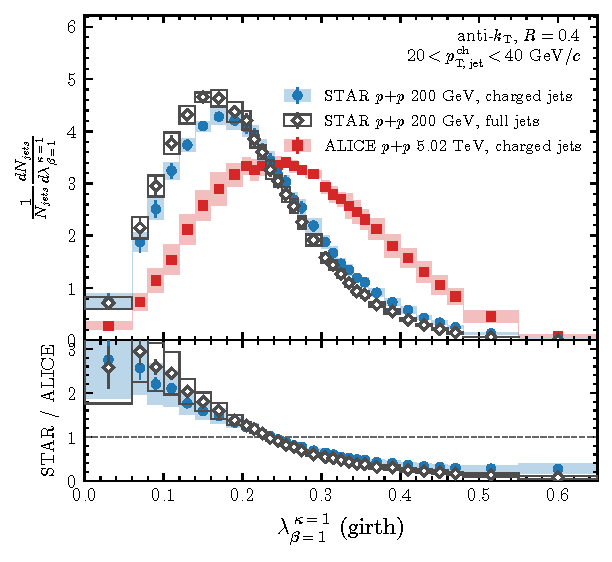
\includegraphics[height=0.63\textheight]{angularities/pp/pub_comparison/alice_2107.11303/angularities_noptd/alice_ungroomed_lambda1_ptch20_40.pdf}
	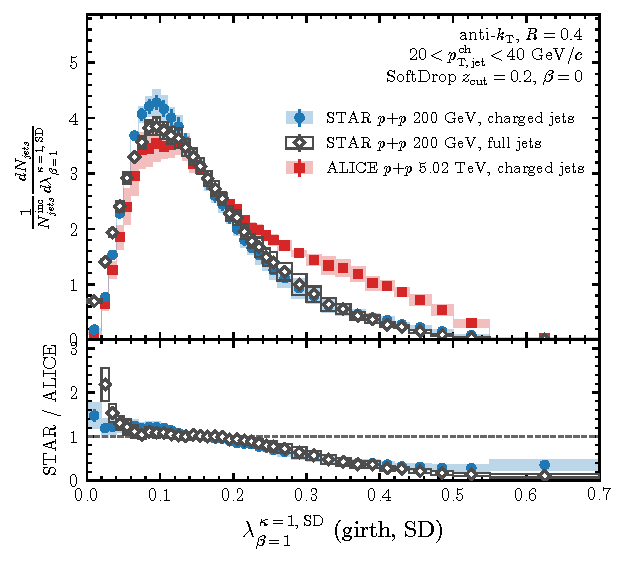
\includegraphics[height=0.63\textheight]{angularities/pp/pub_comparison/alice_2107.11303/angularities_noptd/alice_groomed_lambda1_ptch20_40.pdf}
	\begin{itemize}\setlength{\itemsep}{0pt}
		\scriptsize
		\item Charged jets, 20--40~GeV/\(c\), from our unfolded jets
		\item RHIC jets \textbf{much narrower} --- more quark jets
	\end{itemize}
	\refnote{ALICE, JHEP 05 (2022) 061}
\end{frame}

%======================================================================
\section{Summary and outlook}

\begin{frame}{Summary}
	\small
	\begin{itemize}
		\item \textbf{Jet-hadron (published):} no event-plane dependence; path-length effect \(<\) uncertainties
		\item<2-> \textbf{Au+Au angularities:} first unbinned ML unfolding in heavy ions; vacuum-like
		\item<3-> \textbf{\(p+p\) angularities:} first at RHIC; MC too narrow; \Rg profiles: radiation per splitting
		\item<4-> Heavy-ion: \textbf{survivor bias}
		\item<5-> \(p+p\) baseline calculated for inclusive and groomed angularities
		\item<6-> Developed analysis pipeline with unbinned unfoldoing for RHIC
	\end{itemize}
\end{frame}

\begin{frame}{Outlook}
	\begin{itemize}
		\item Groomed angularities, \Rg profiles in \textbf{Au+Au}
		\item<3-> STAR paper: inclusive/groomed angularities in \(p+p\)
	\end{itemize}
\end{frame}

%\begin{frame}{Acknowledgements}
%	\begin{columns}[c]
%		\begin{column}{0.64\textwidth}
%			\small
%			\begin{itemize}
%				\item \textbf{Prof. Sevil Salur} --- like Athena, always looking out for me.
%				\item \textbf{The committee}: Prof. Matthew R. Buckley, Prof. John P. Hughes, Prof. Ronald D. Ransome, Dr. Isaac A. Mooney --- who made me believe in \emph{xenia} again.
%				\item \textbf{Prof. Bedangadas Mohanty} --- my Nestor, before the voyage began.
%				\item \textbf{Dr. Joel A. Mazer}, the STAR Collaboration, and Sevil's group: Khovesh Ramdin, Ravi Koka, Jinglin Liu.
%				\item \textbf{Claire}, my family --- and Janeway and Bones.
%			\end{itemize}
%		\end{column}
%		\begin{column}{0.32\textwidth}
%			\centering
%			
\includegraphics[height=1.2cm]{figures/logos/DOE}\\[4mm]
%			
\includegraphics[height=1.2cm]{figures/logos/NSF}\\[4mm]
%			
\includegraphics[height=1.2cm]{figures/logos/STAR}
%		\end{column}
%	\end{columns}
%\end{frame}

\begin{frame}
	\centering
	\vfill
	{\Huge\color{PrimaryColor} Thank you}\\[6mm]
	%	{\large\itshape Ithaka gave you the marvelous journey.}\\[2mm]
	%	{\small --- C.\,P.~Cavafy, \emph{Ithaka}}
	\vfill
\end{frame}

%======================================================================
\appendix

\begin{frame}
	\centering\Huge\color{PrimaryColor} Backup
\end{frame}

\begin{frame}{Backup: statistical uncertainties from replicas}
	\begin{itemize}
		\item Replica = full unfolding: \(w^{(r)}_n = \prod_k \nu^{(r)}_k\)
		\item Subsample to train, evaluate on all jets
		\item \(\bar H\) = mean, \(\sigma_H\) = std over replicas; ratios per replica
		\item \(\sigma_H\): data + MC stat.\ + training; conservative
		\item Barlow: keep shift if \(|\Delta \bar H| \geq \sqrt{|\sigma^2_\mathrm{var} - \sigma^2_\mathrm{nom}|}\)
	\end{itemize}
\end{frame}

\begin{frame}{Backup: vectorized ensemble training (\texttt{torchstrap})}
	\centering
	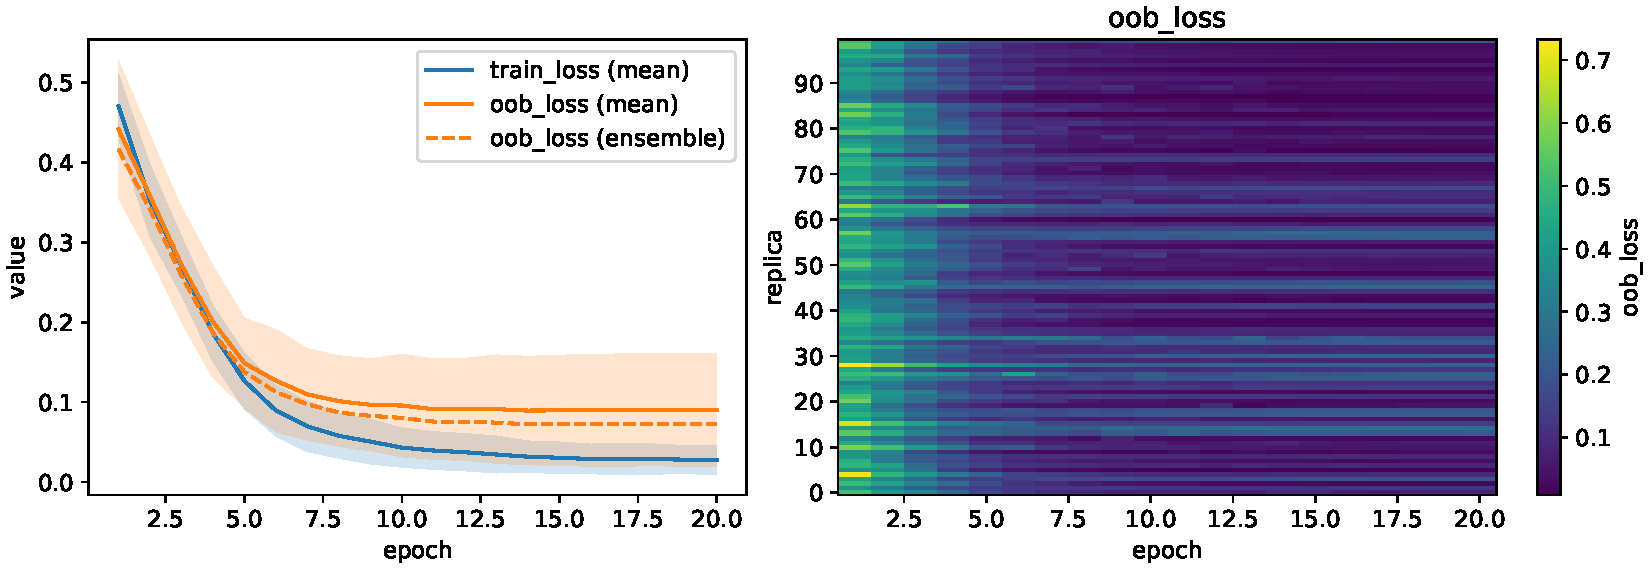
\includegraphics[width=0.48\linewidth]{torchstrap/spirals_training.pdf}
	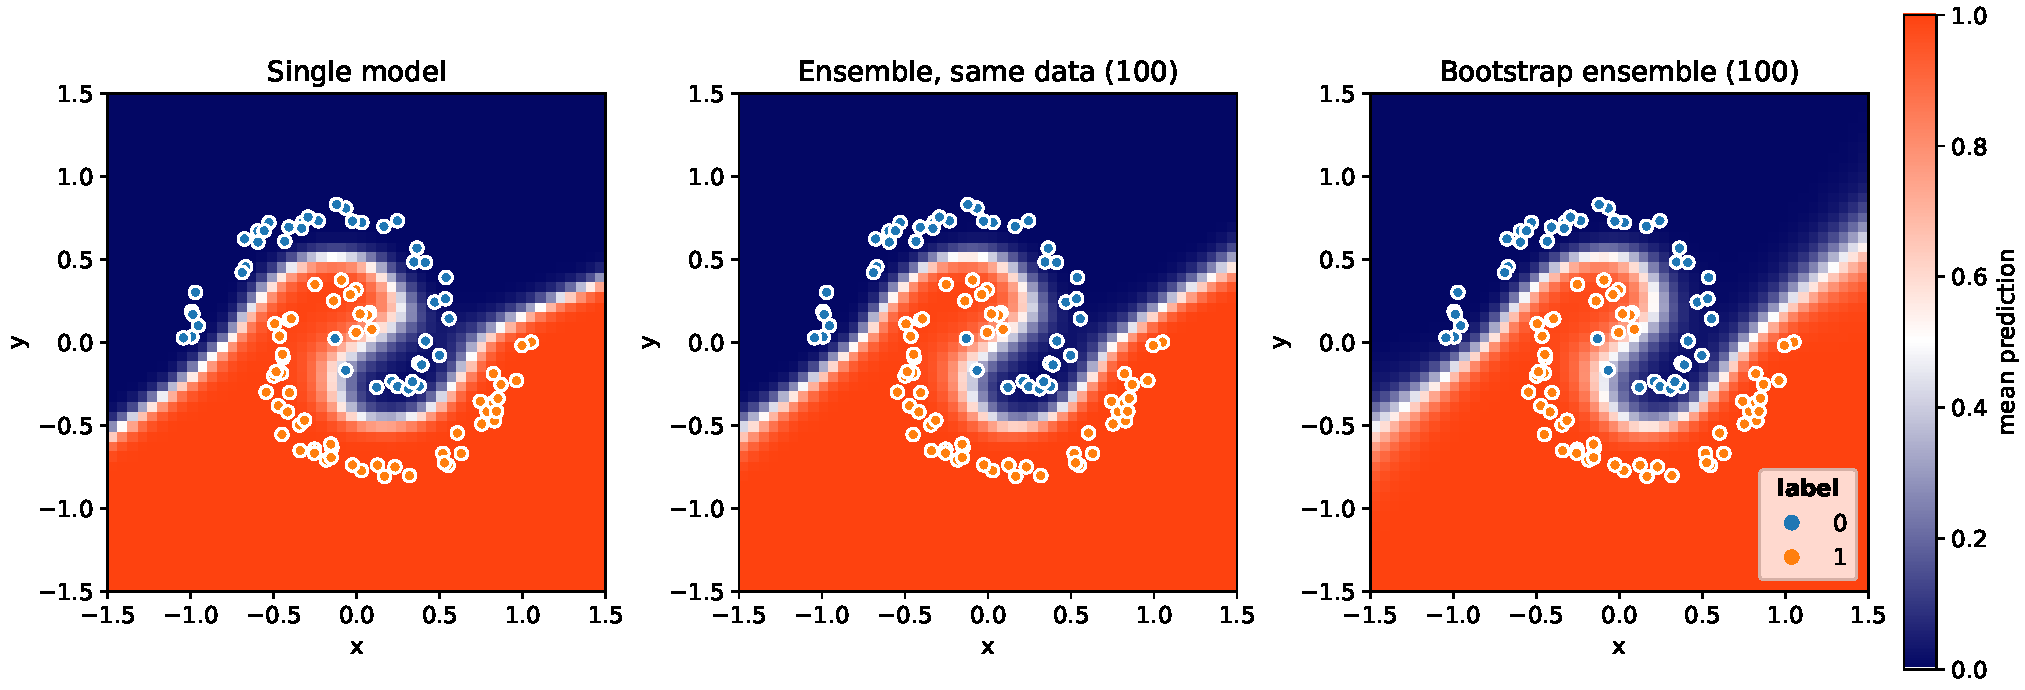
\includegraphics[width=0.48\linewidth]{torchstrap/spirals_predictions.pdf}
	\begin{itemize}
		\small
		\item Stateless models, \texttt{vmap} over replicas, fused Adam
	\end{itemize}
\end{frame}

\begin{frame}{Backup: systematics, inclusive distributions}
	\centering
	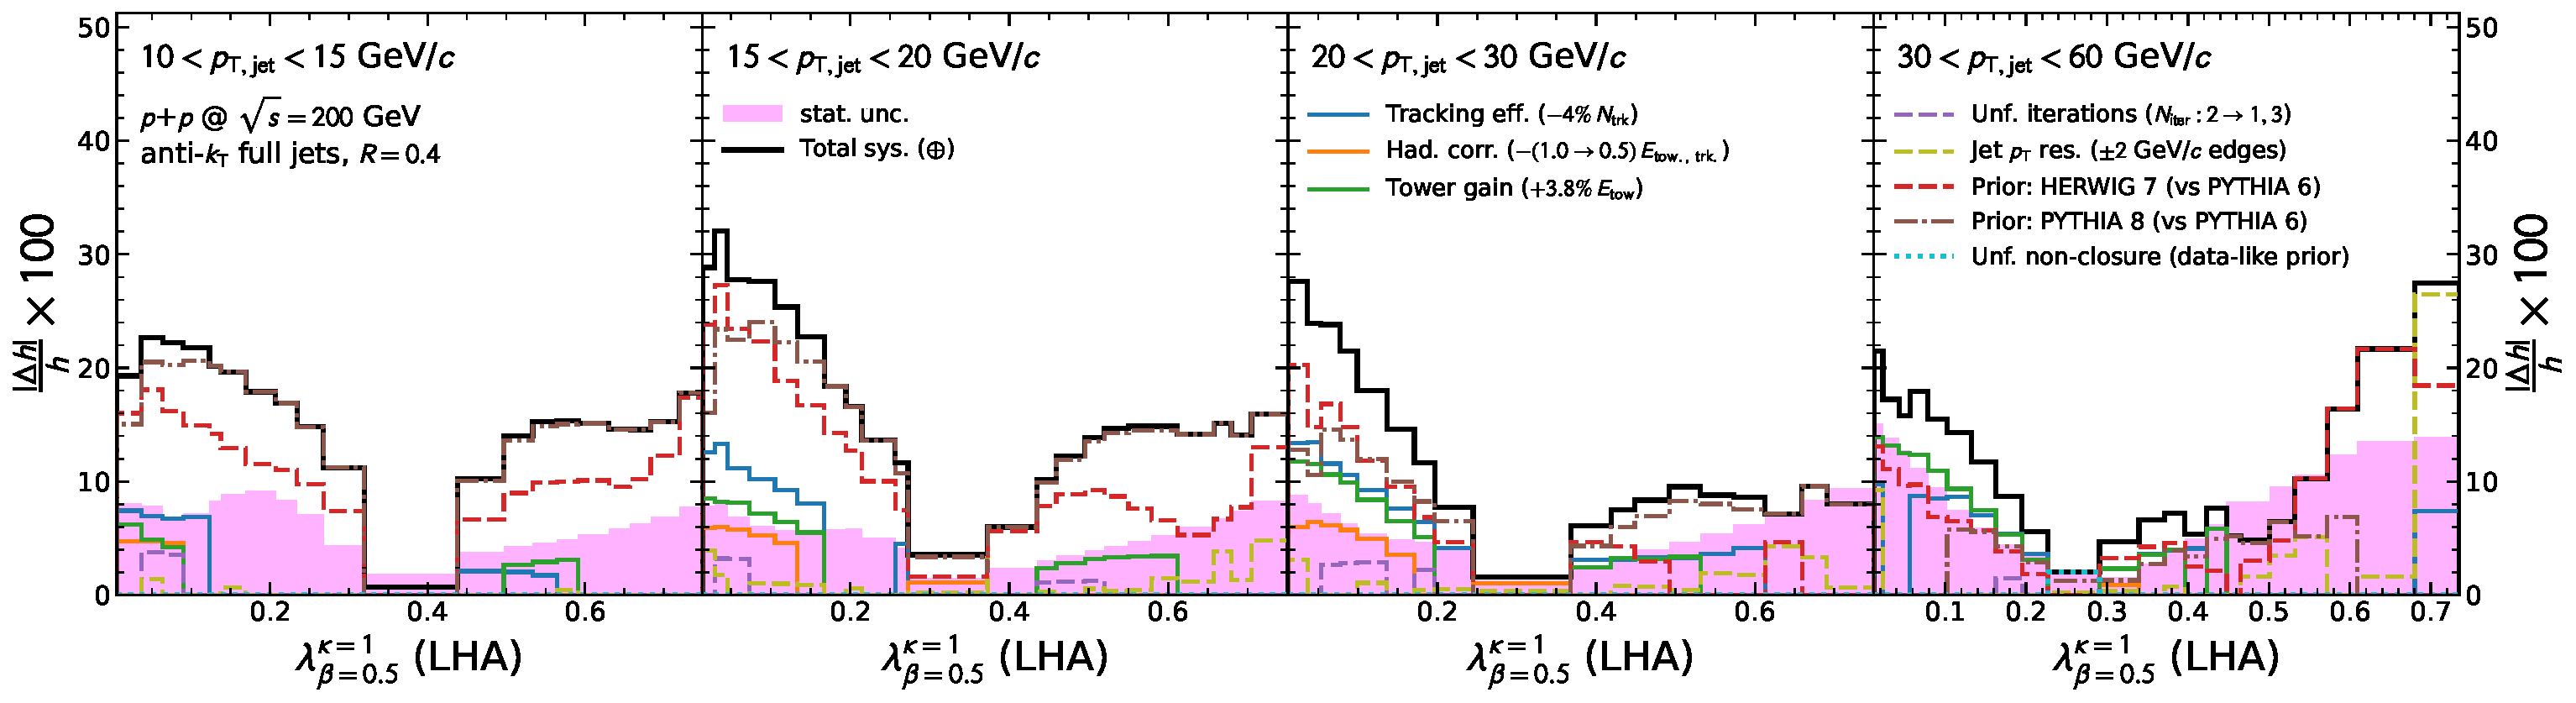
\includegraphics[width=0.85\linewidth]{angularities/pp/sys_ch_ang_k1_b0.5_hist_ang.pdf}\\
	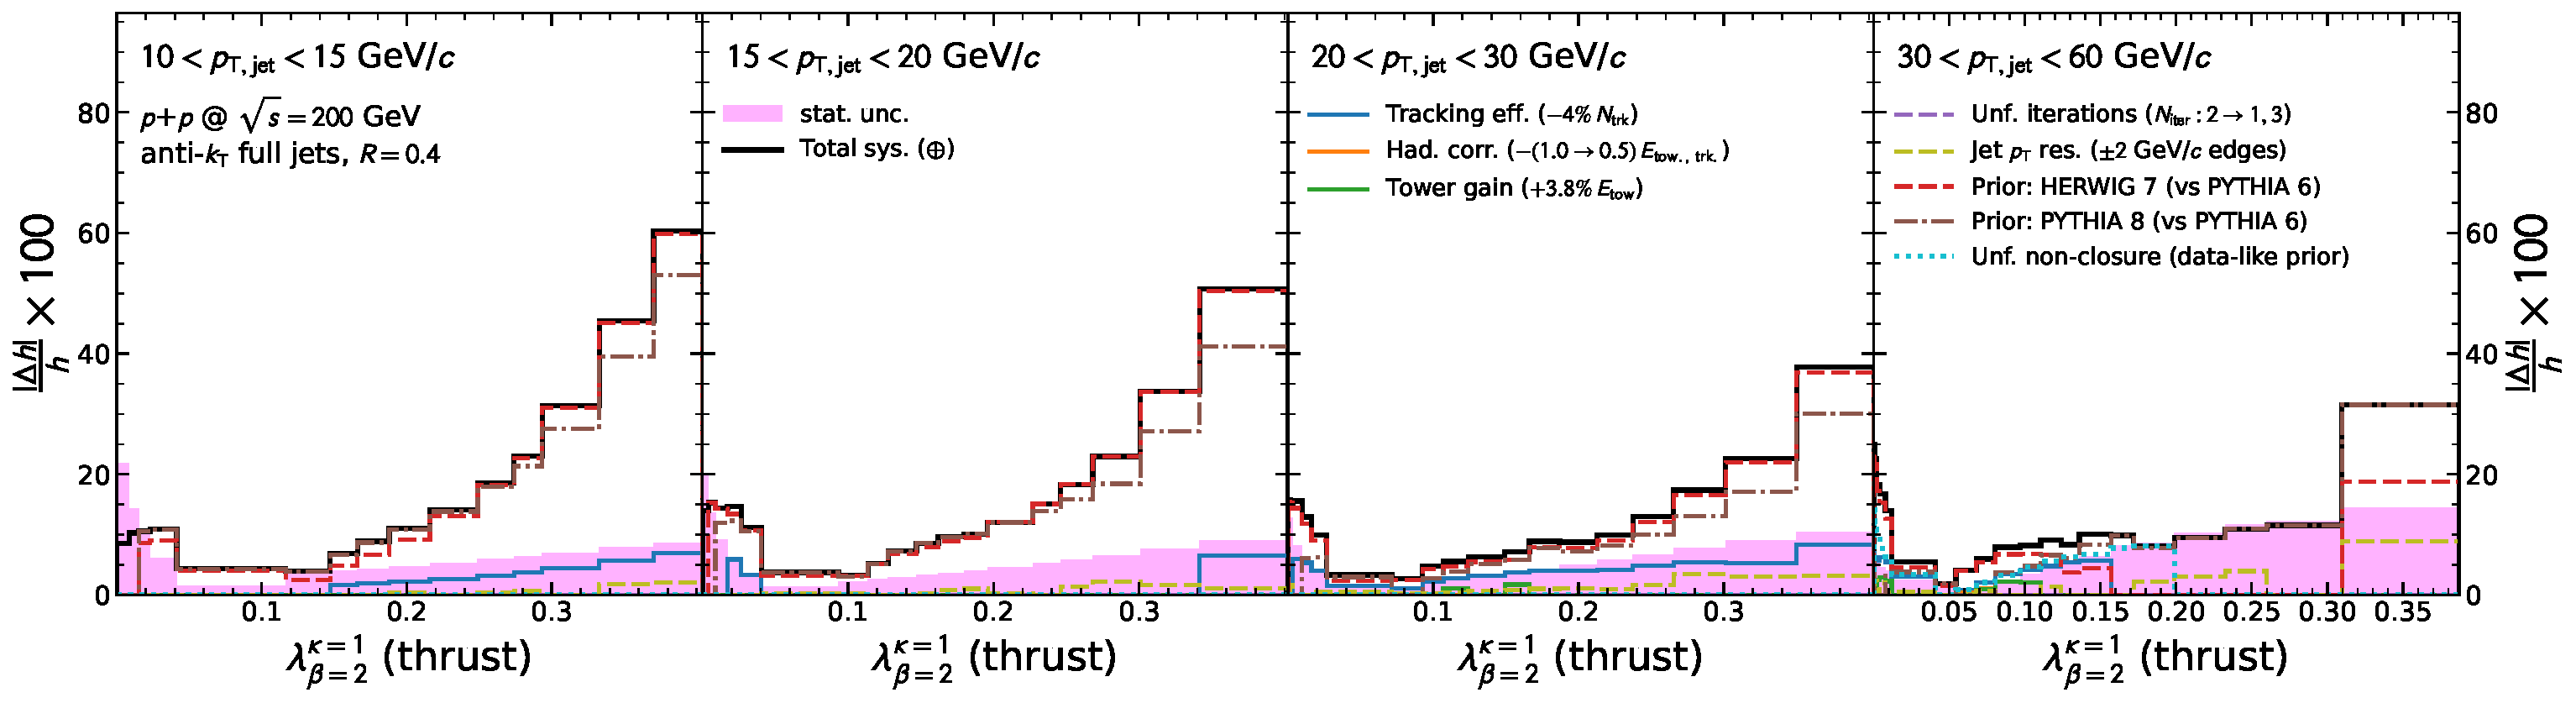
\includegraphics[width=0.85\linewidth]{angularities/pp/sys_ch_ang_k1_b2_hist_ang.pdf}
\end{frame}

\begin{frame}{Backup: systematics, groomed distributions}
	\centering
	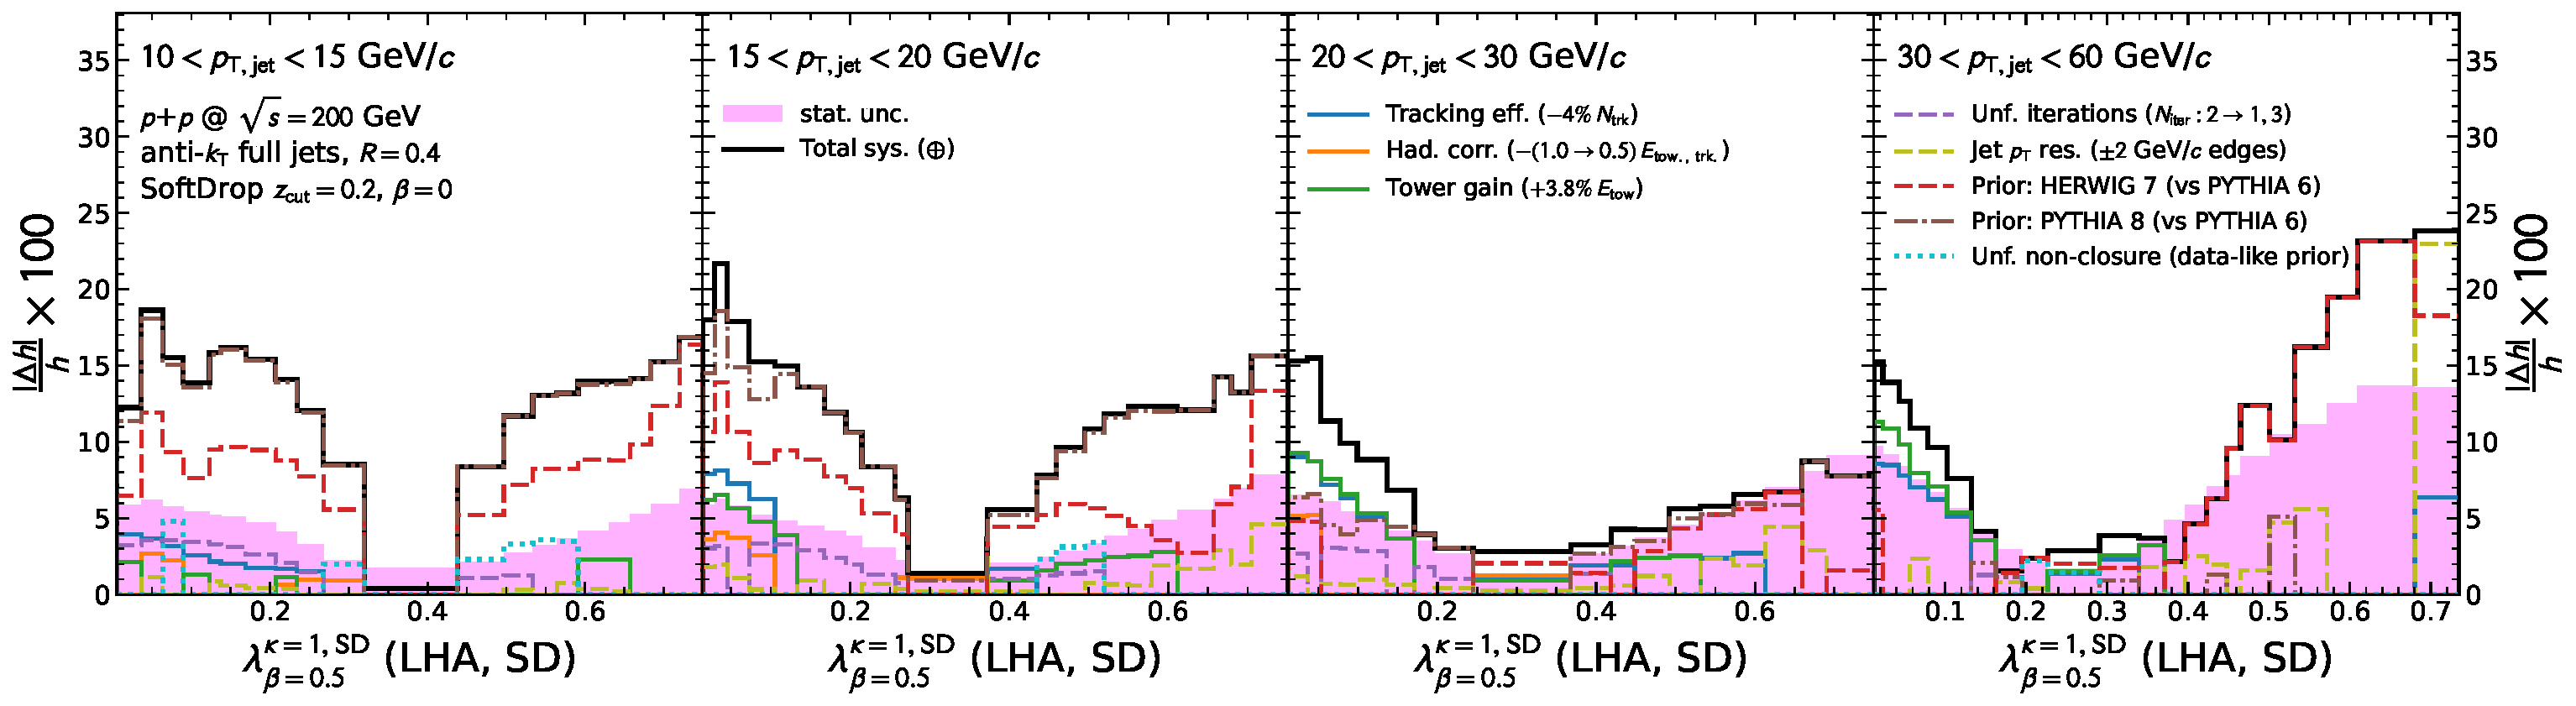
\includegraphics[height=0.26\textheight]{angularities/pp/sys_ch_ang_k1_b0.5_hist_sd_ang.pdf}\\
	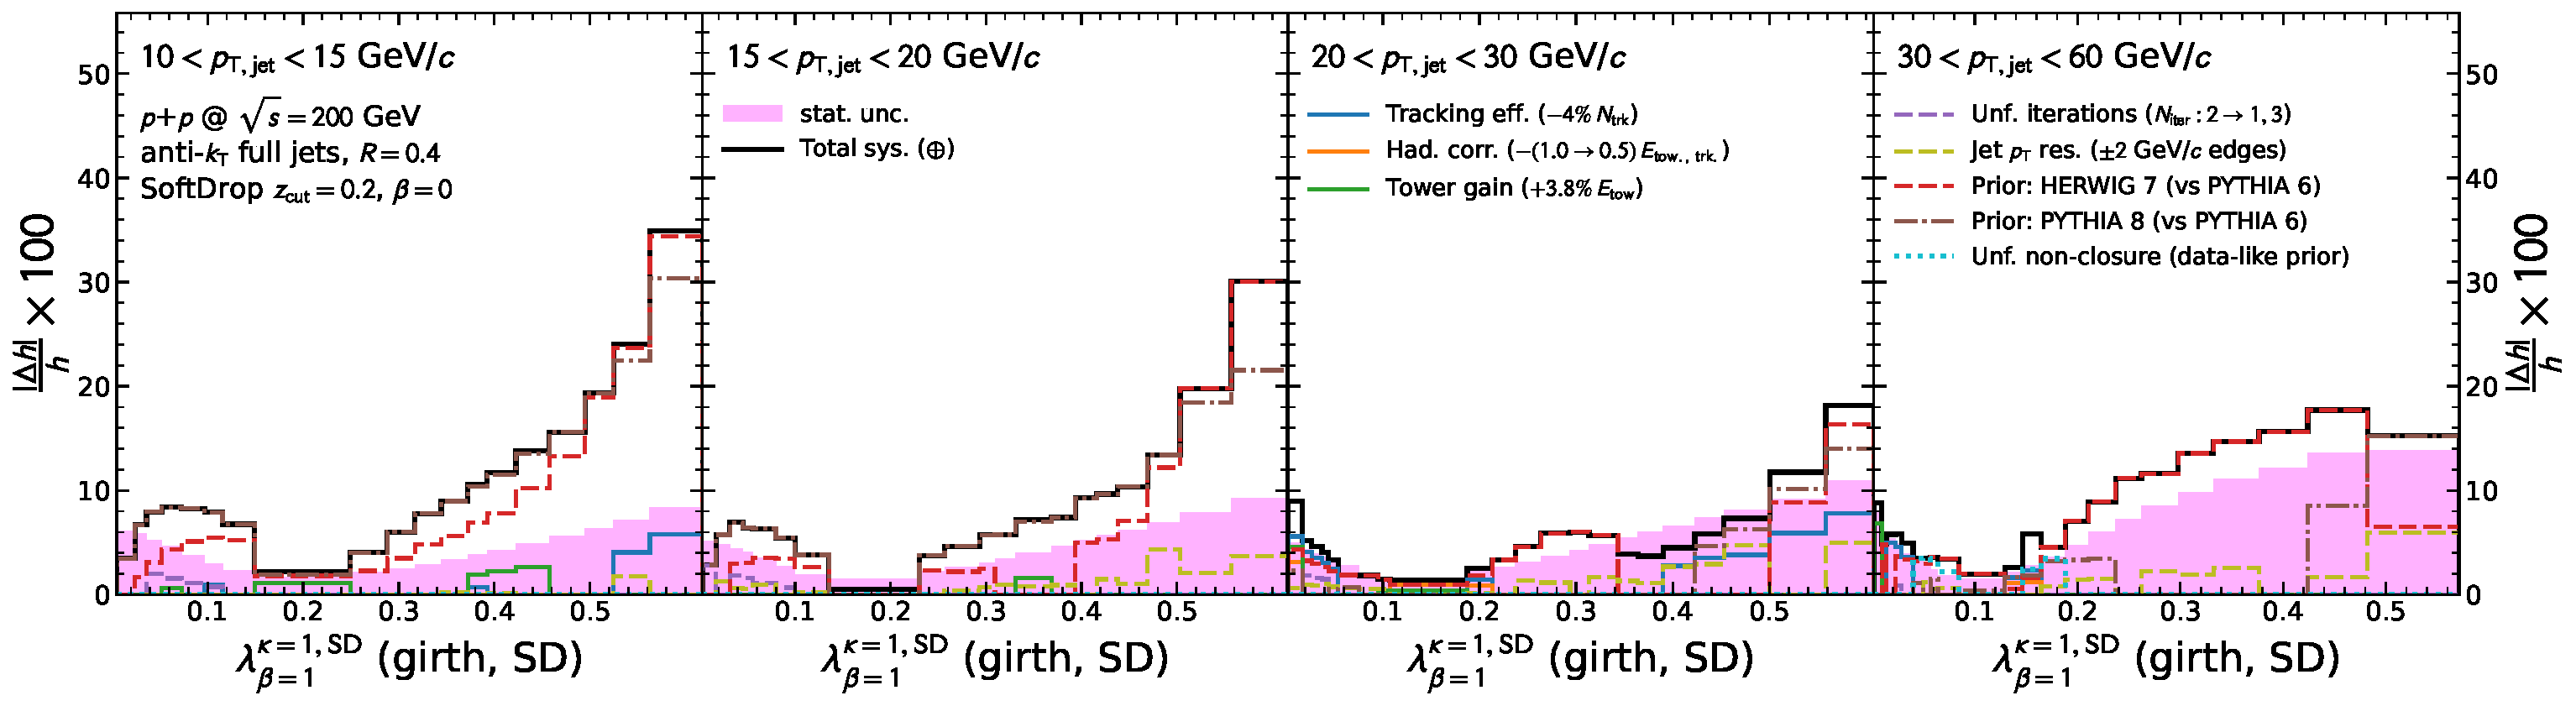
\includegraphics[height=0.26\textheight]{angularities/pp/sys_ch_ang_k1_b1_hist_sd_ang.pdf}\\
	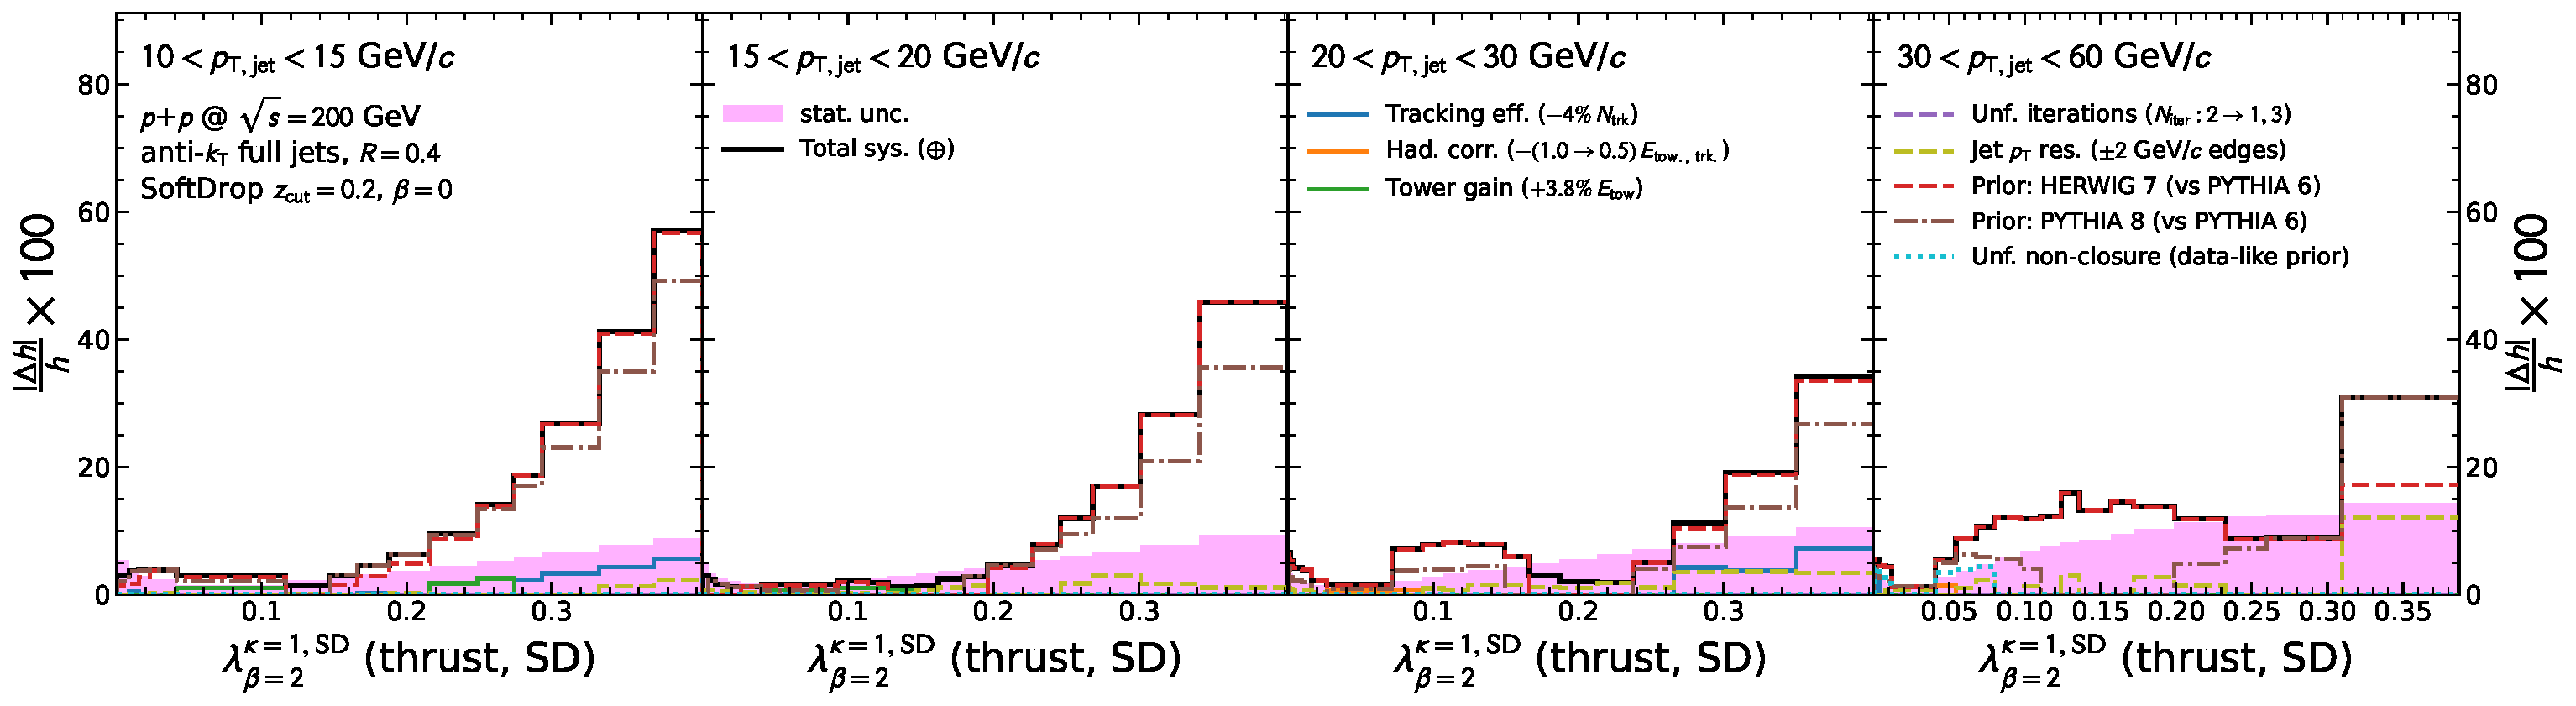
\includegraphics[height=0.26\textheight]{angularities/pp/sys_ch_ang_k1_b2_hist_sd_ang.pdf}
\end{frame}

\begin{frame}{Backup: systematics, \Rg profiles}
	\centering
	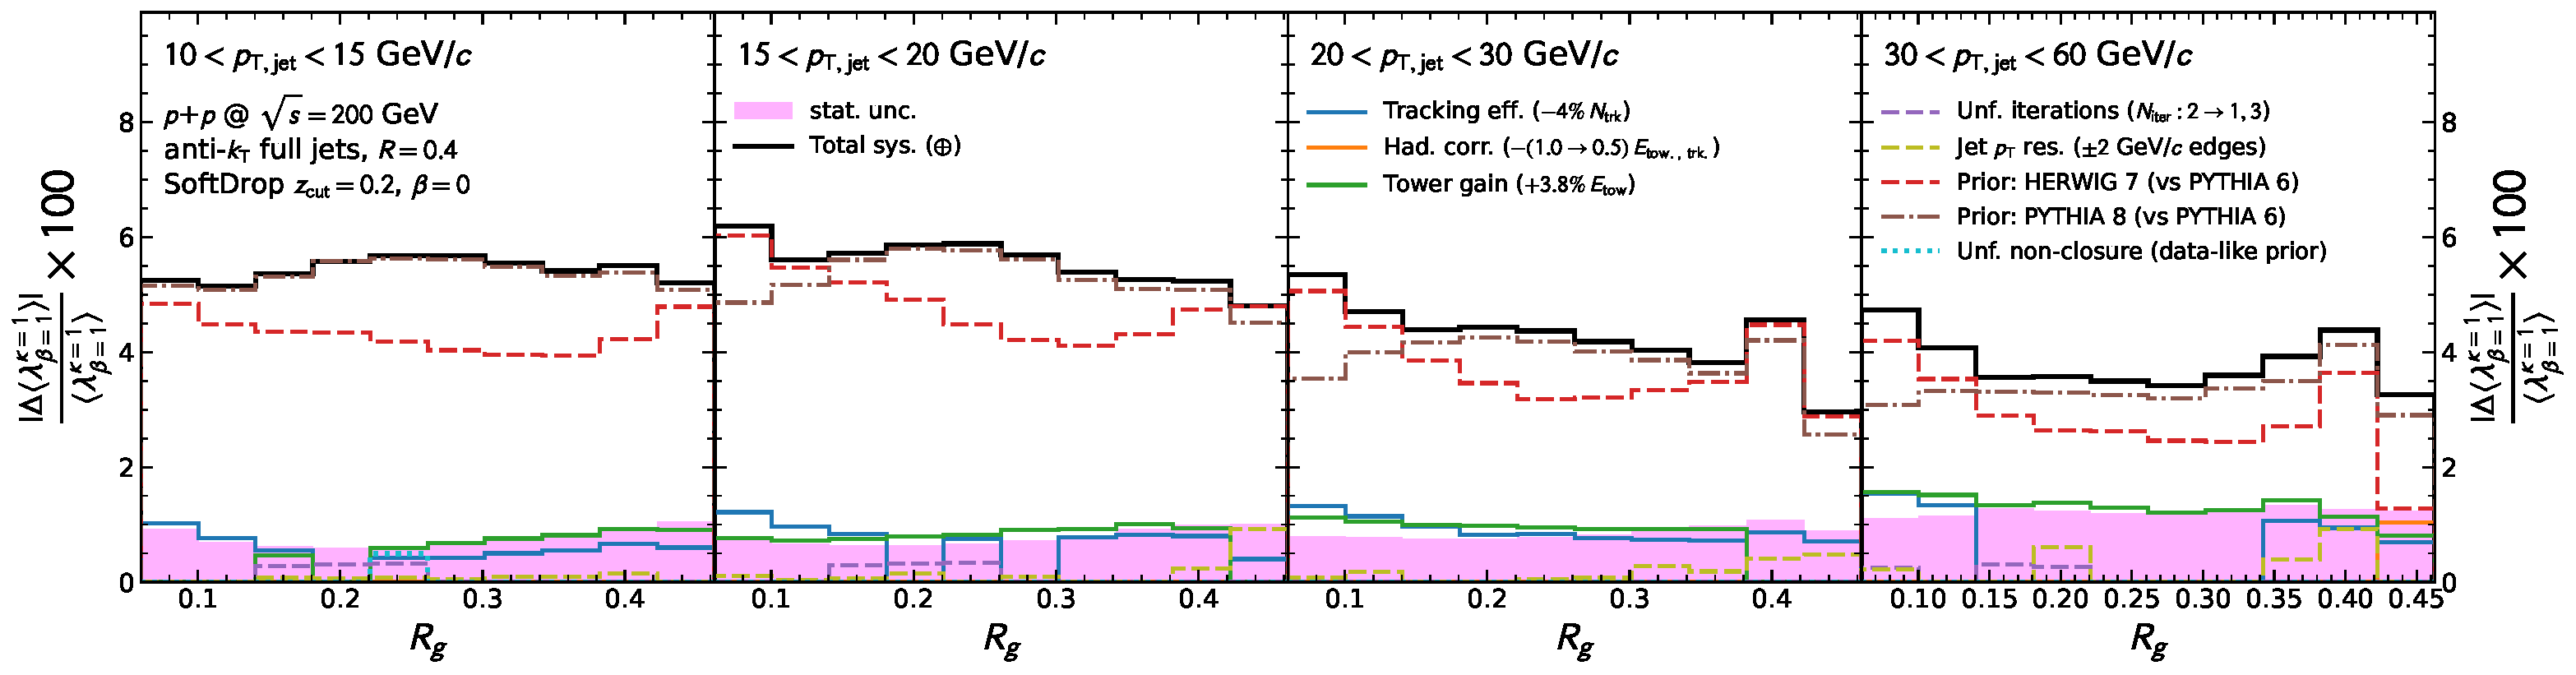
\includegraphics[width=0.85\linewidth]{angularities/pp/sys_ch_ang_k1_b1_prof_incl_vs_sd_dR.pdf}\\
	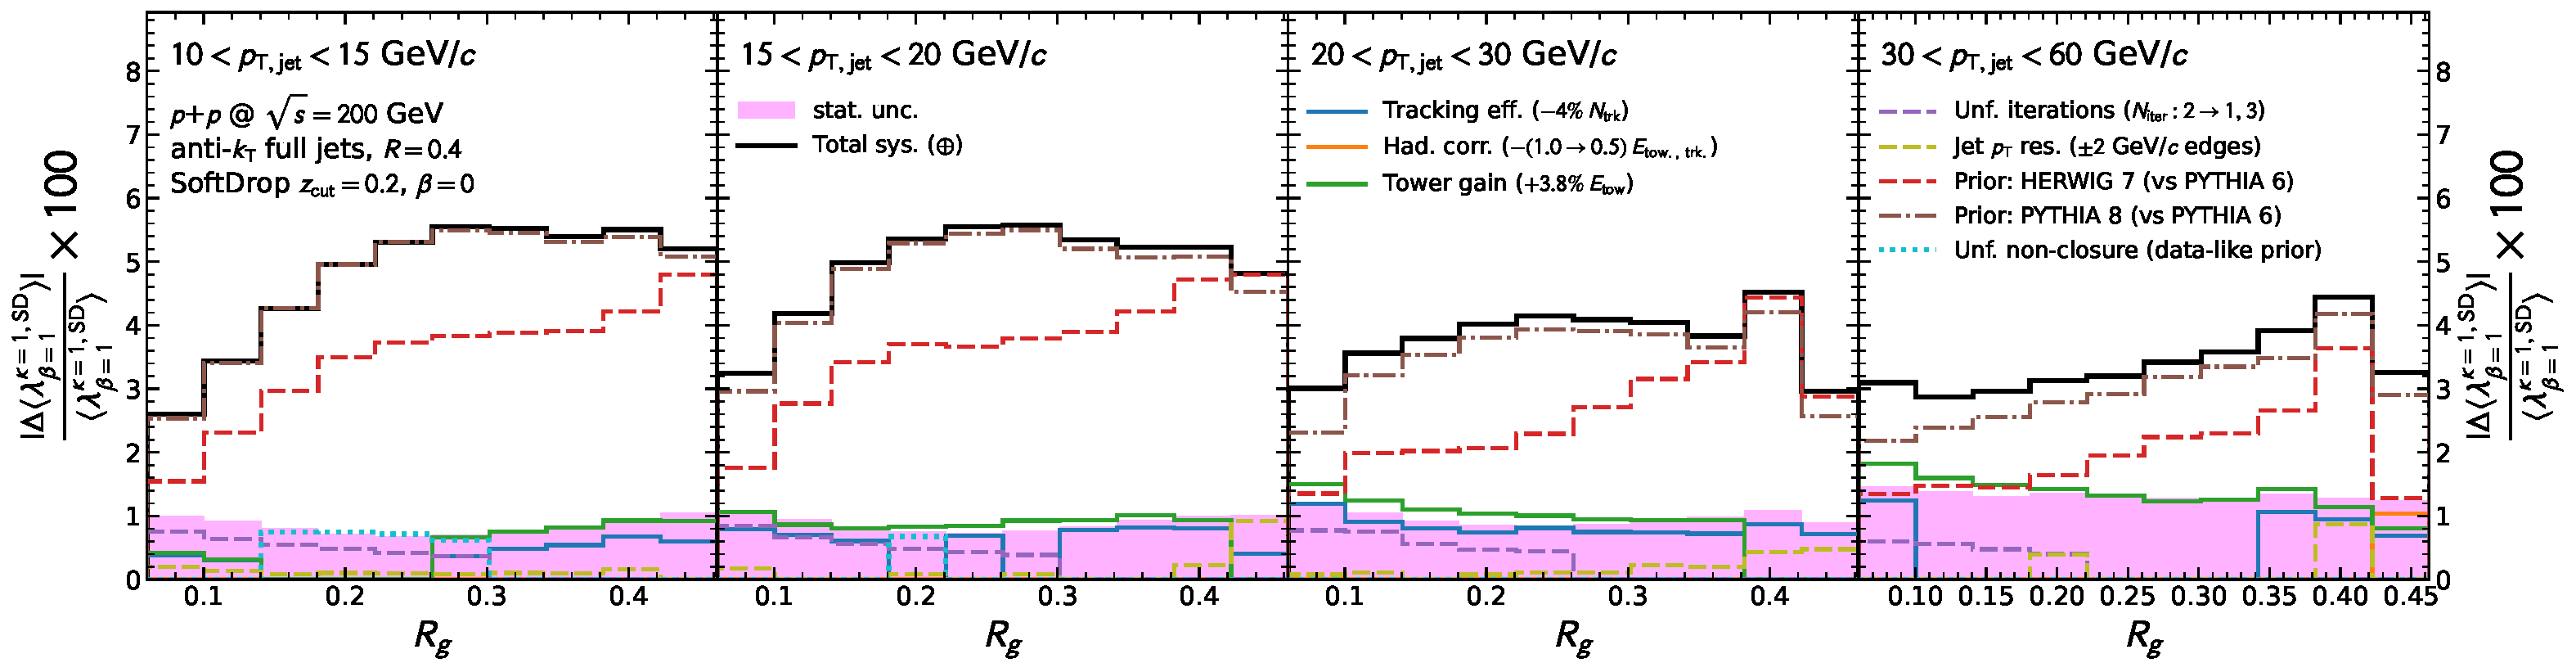
\includegraphics[width=0.85\linewidth]{angularities/pp/sys_ch_ang_k1_b1_prof_sd_vs_sd_dR.pdf}
\end{frame}

\begin{frame}{Backup: prior variation by classifier reweighting}
	\centering
	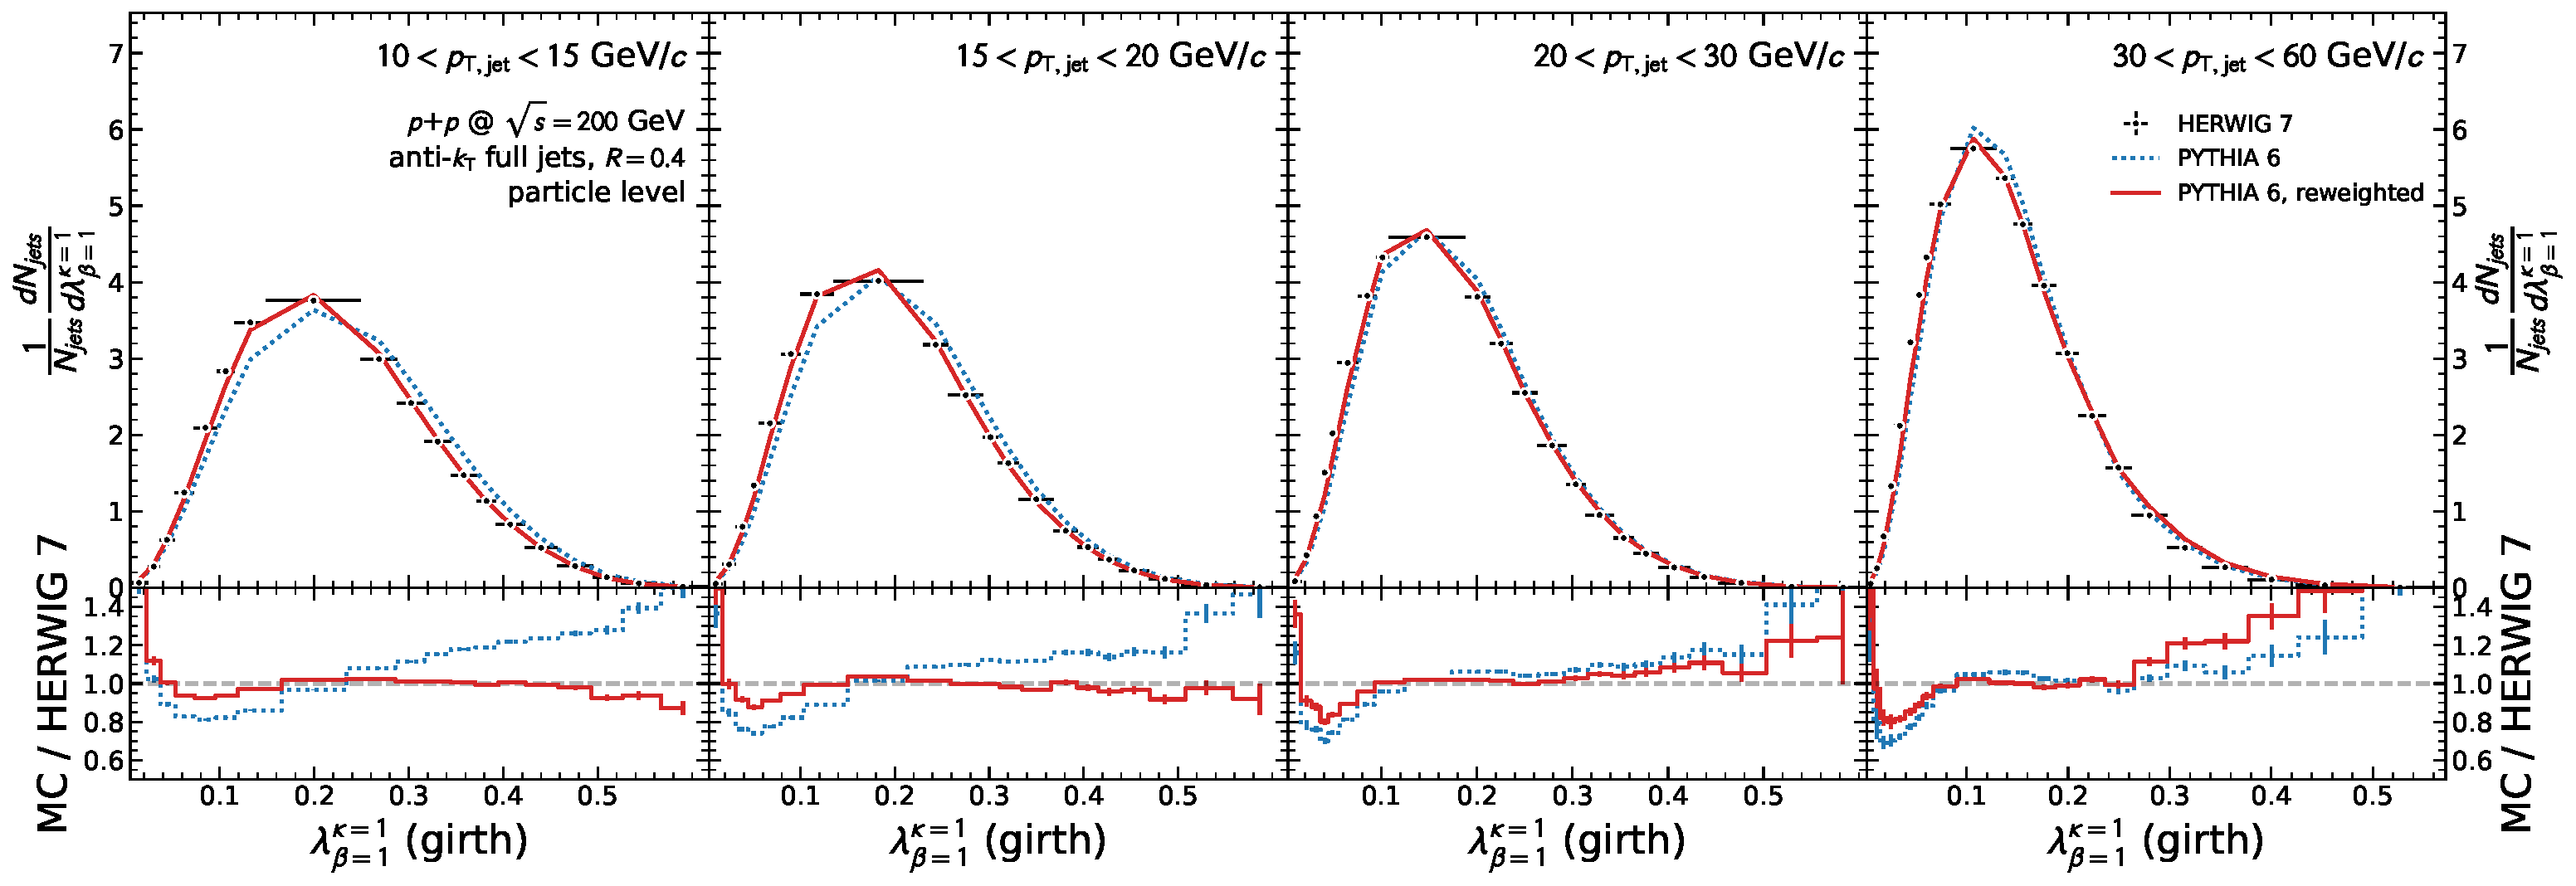
\includegraphics[width=0.49\linewidth]{angularities/pp/reweight_herwig7_ch_ang_k1_b1.pdf}
	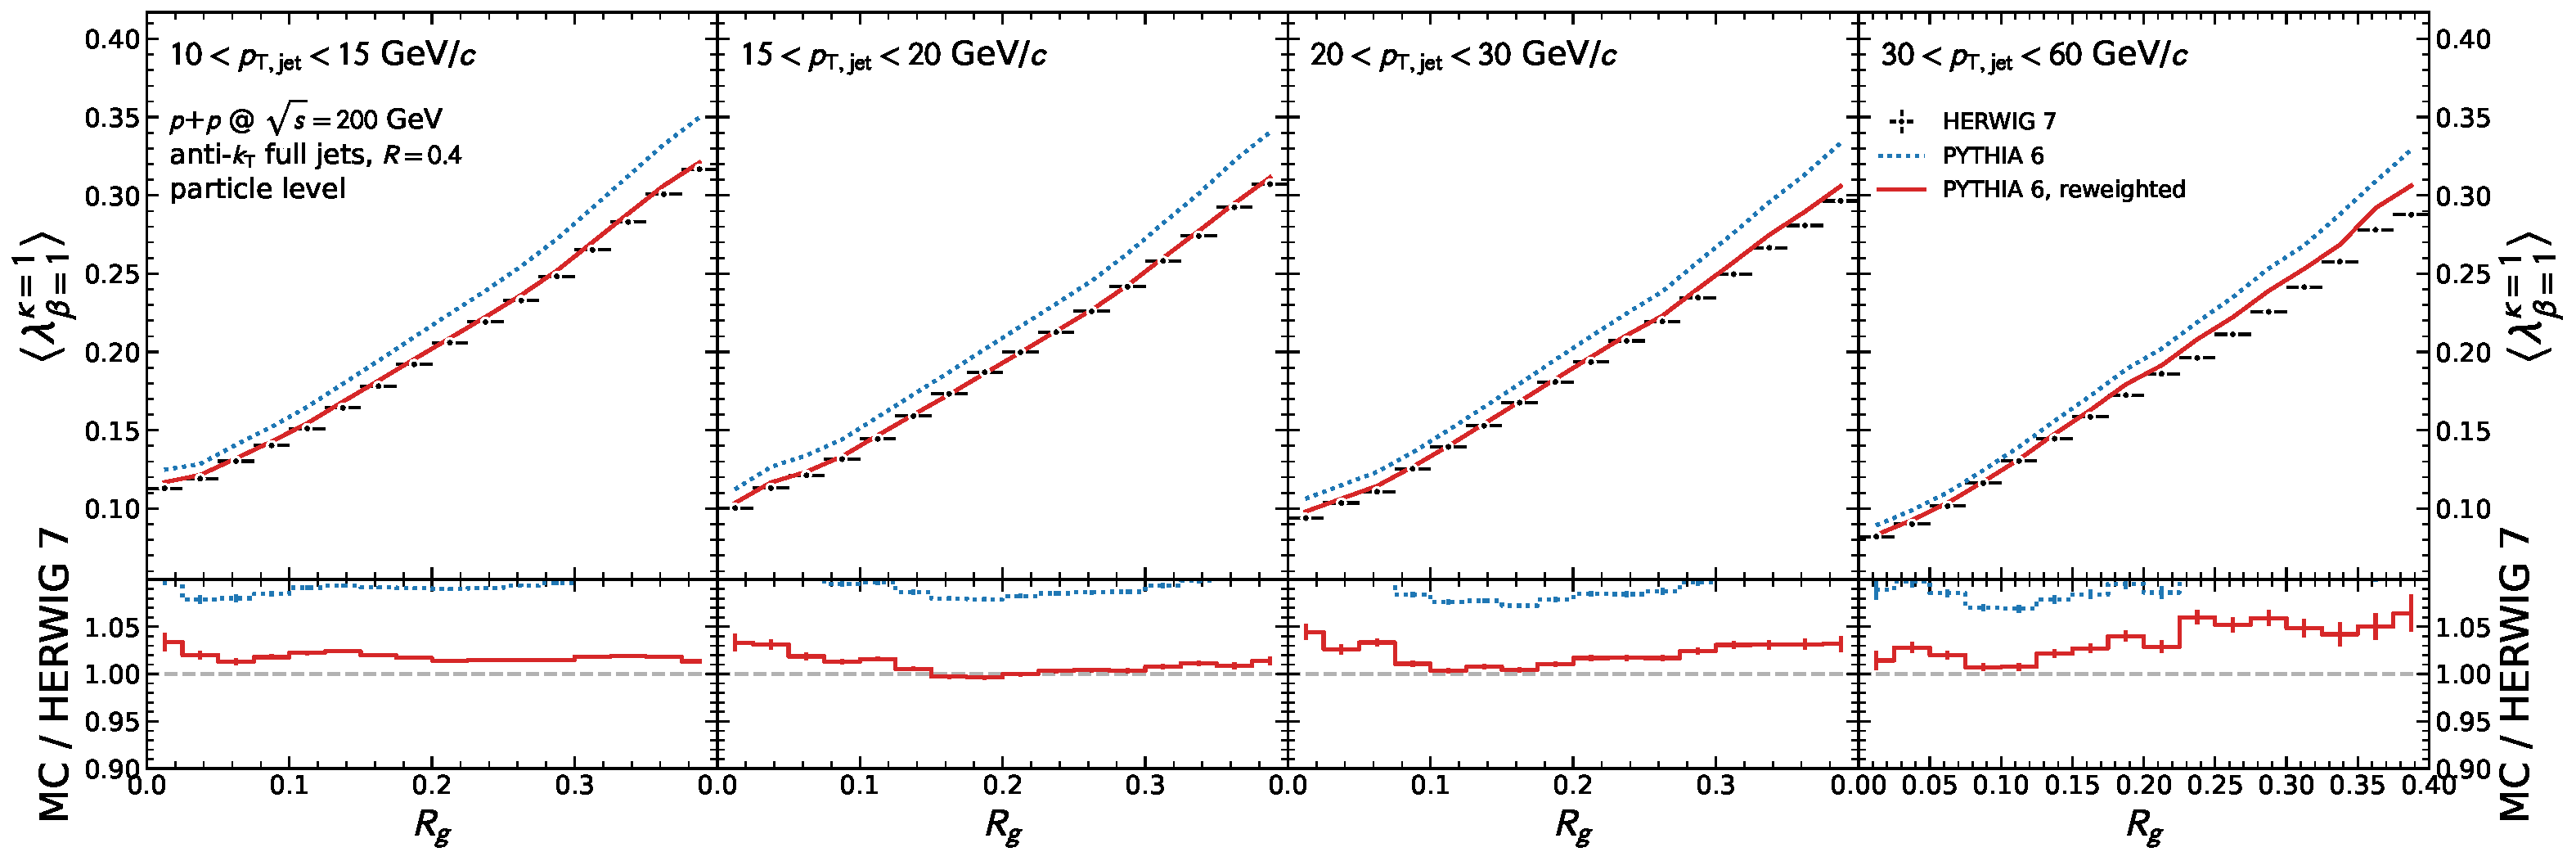
\includegraphics[width=0.49\linewidth]{angularities/pp/reweight_herwig7_prof_ch_ang_k1_b1.pdf}
	\begin{itemize}
		\small
		\item \PYsix \(\to\) \HWseven / \PYeight via classifier on \textbf{all features}; response fixed
		\item<2-> Few-\% match, \alert{incl.\ \Rg correlation} (1-D can't)
	\end{itemize}
\end{frame}

\begin{frame}{Backup: \PYeight prior reweighting}
	\centering
	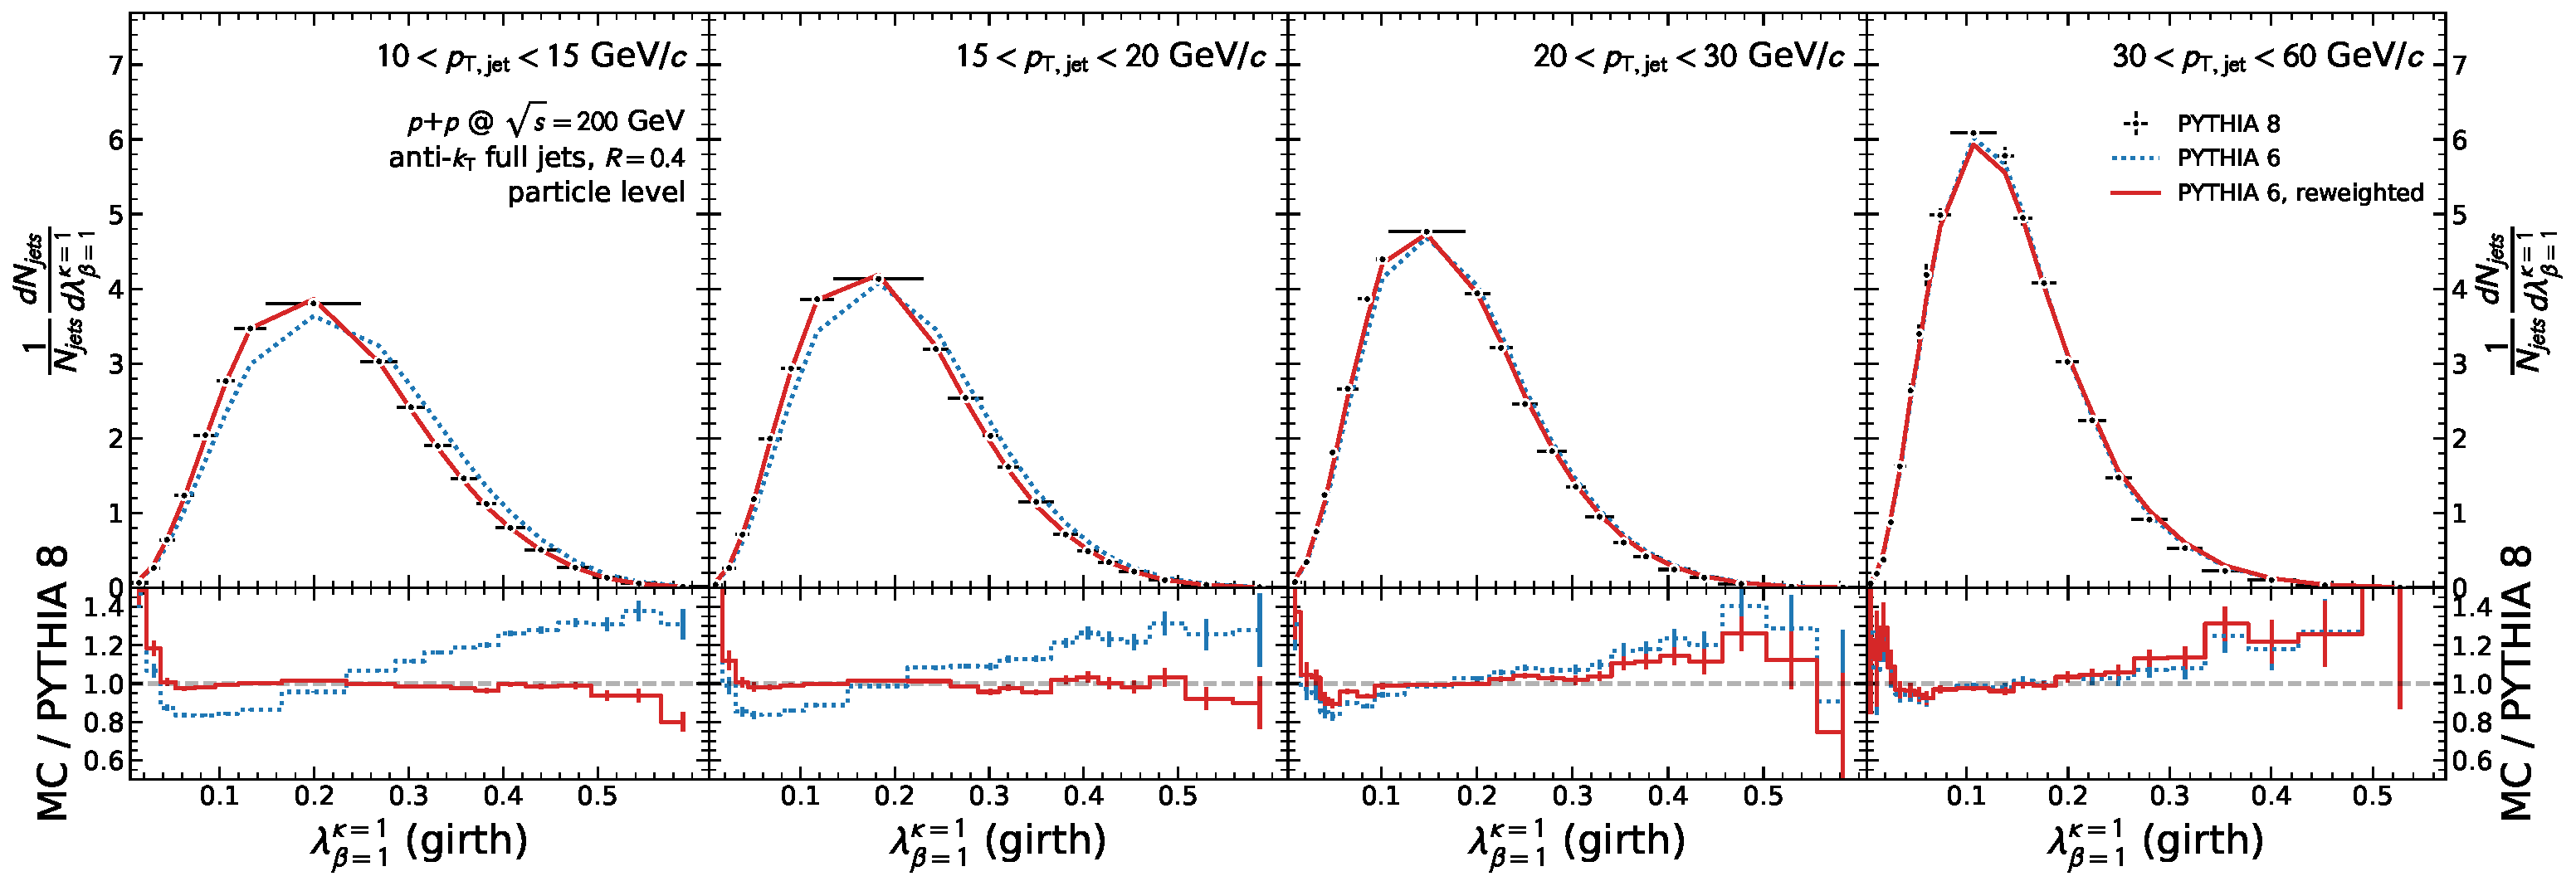
\includegraphics[width=0.49\linewidth]{angularities/pp/reweight_pythia8_ch_ang_k1_b1.pdf}
	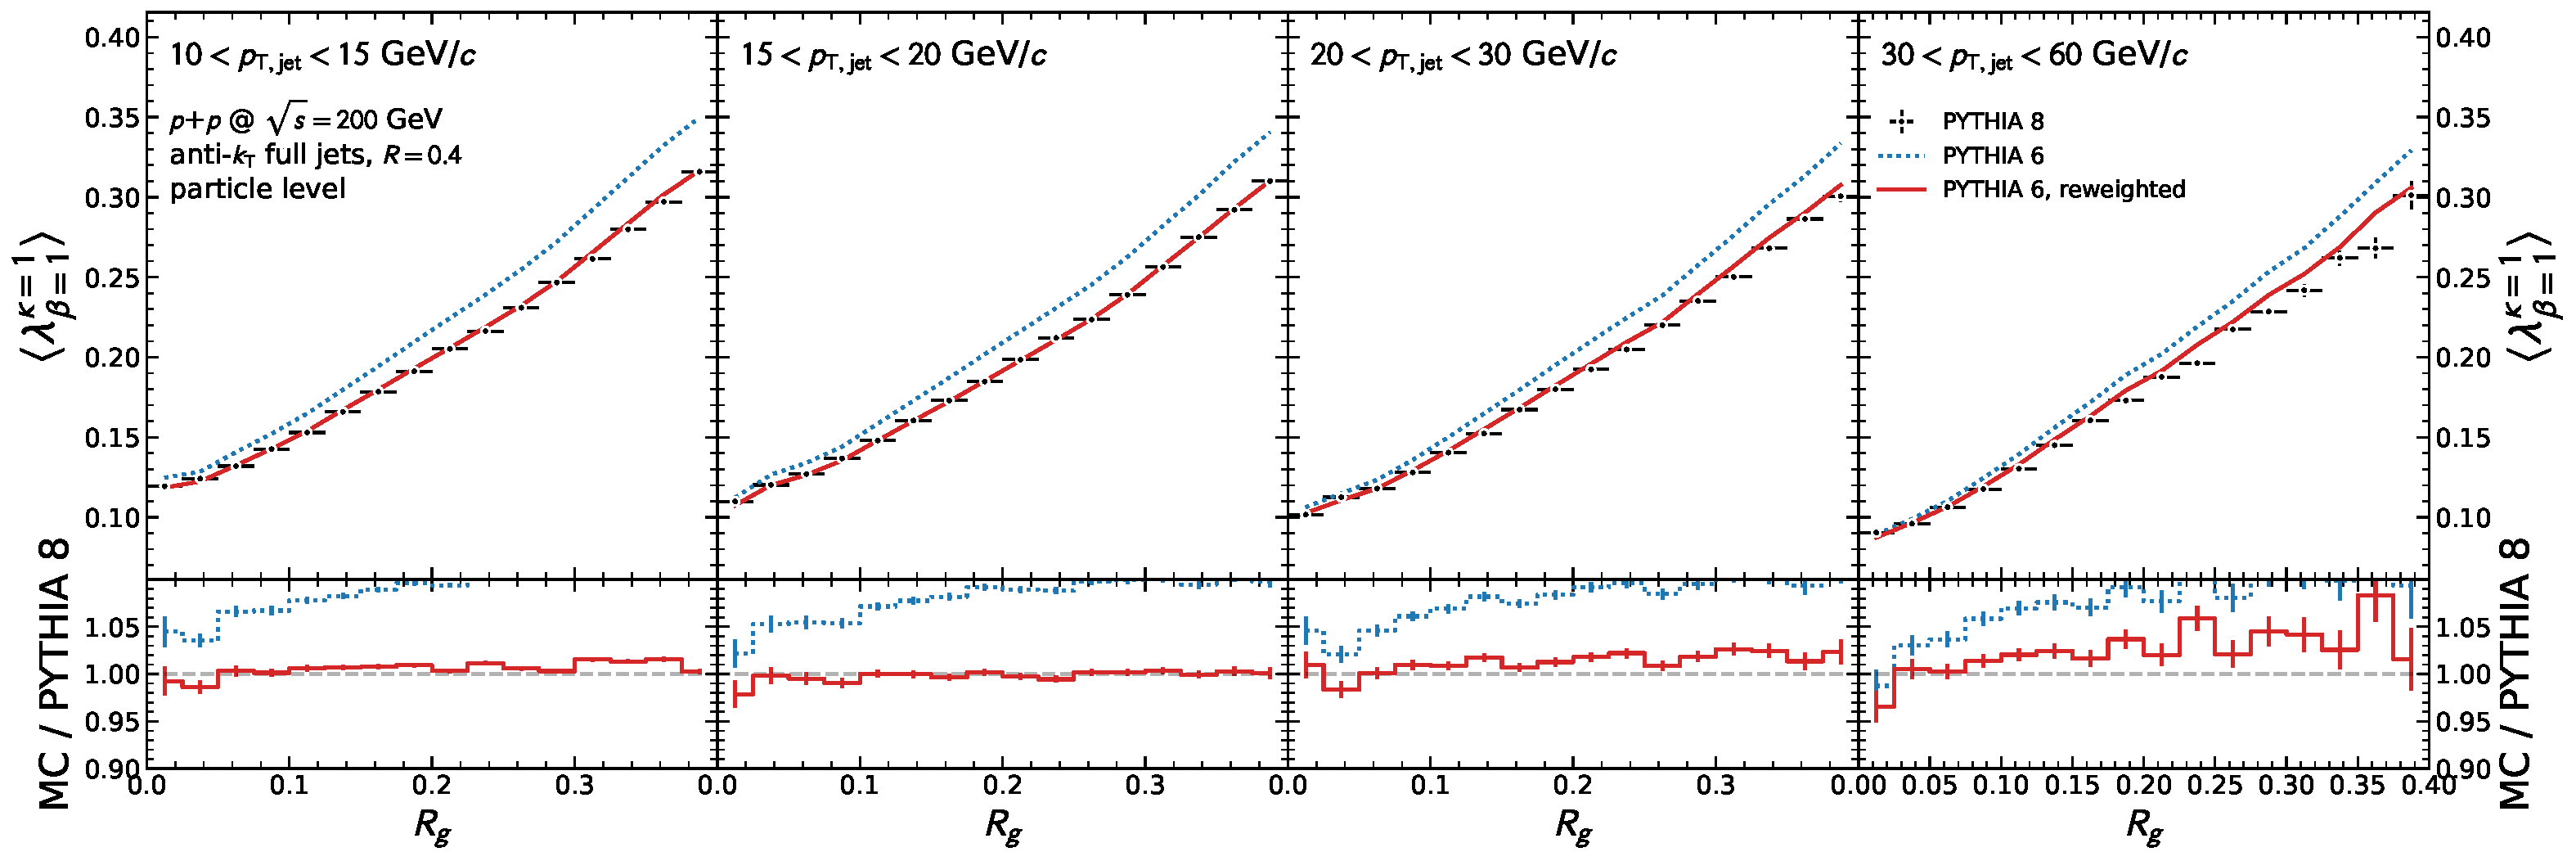
\includegraphics[width=0.49\linewidth]{angularities/pp/reweight_pythia8_prof_ch_ang_k1_b1.pdf}
\end{frame}

\begin{frame}{Backup: ALICE comparison, \(\lambda_2\)}
	\centering
	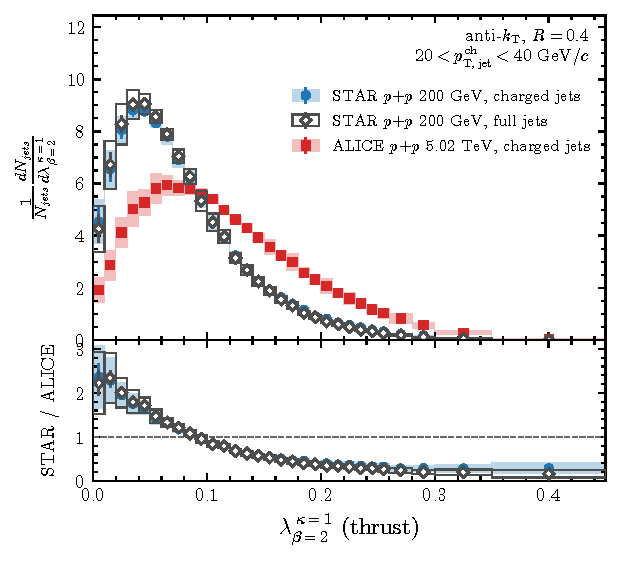
\includegraphics[width=0.4\linewidth]{angularities/pp/pub_comparison/alice_2107.11303/angularities_noptd/alice_ungroomed_lambda2_ptch20_40.pdf}
	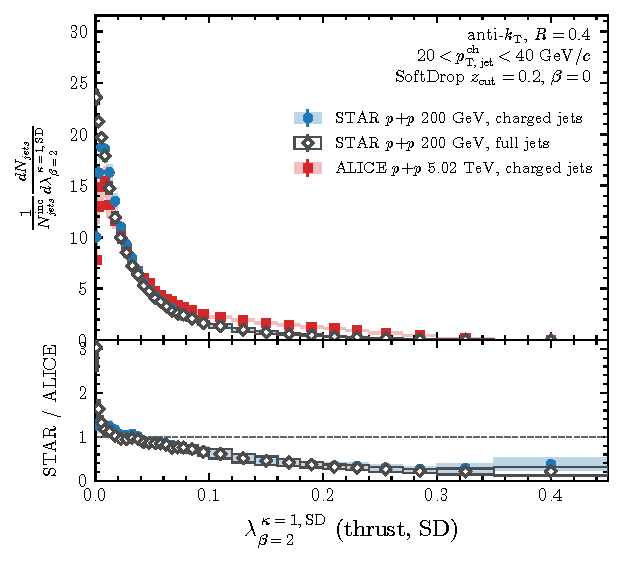
\includegraphics[width=0.4\linewidth]{angularities/pp/pub_comparison/alice_2107.11303/angularities_noptd/alice_groomed_lambda2_ptch20_40.pdf}
\end{frame}

\begin{frame}{Backup: cross-check with published STAR observables}
	\centering
	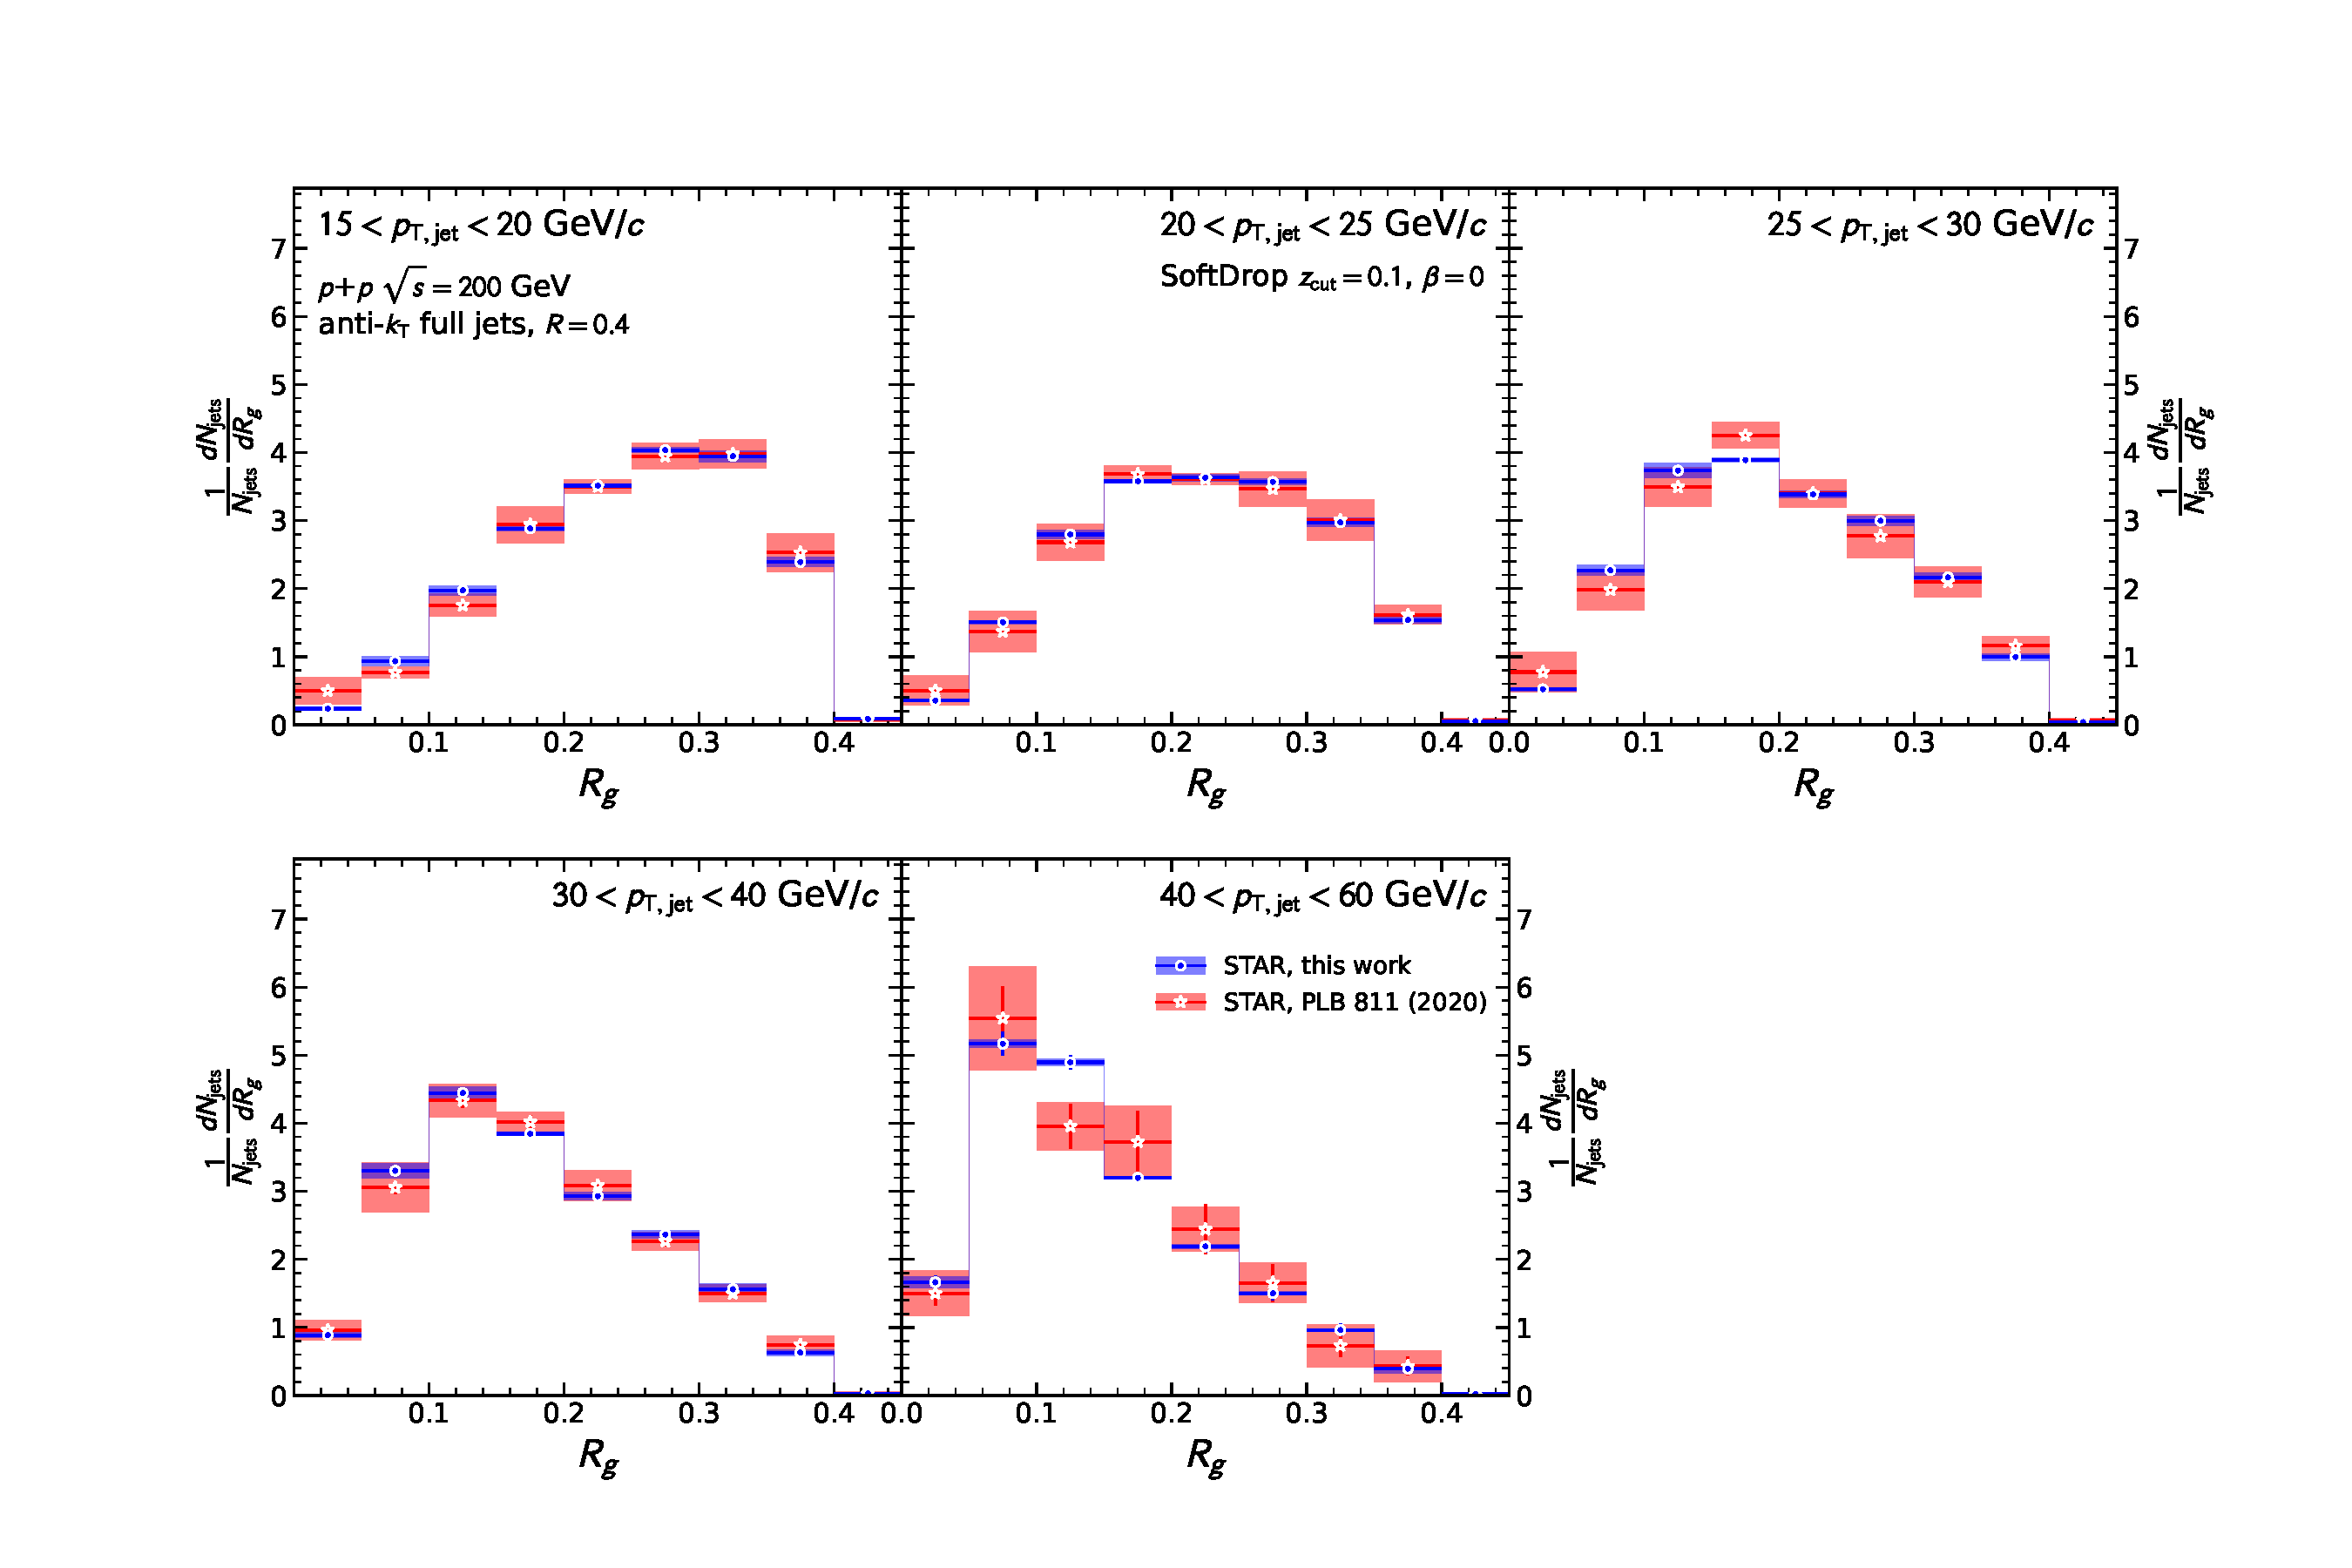
\includegraphics[width=0.495\linewidth]{angularities/pp/pub_comparison/star_published/star_pub_sd_dR}
	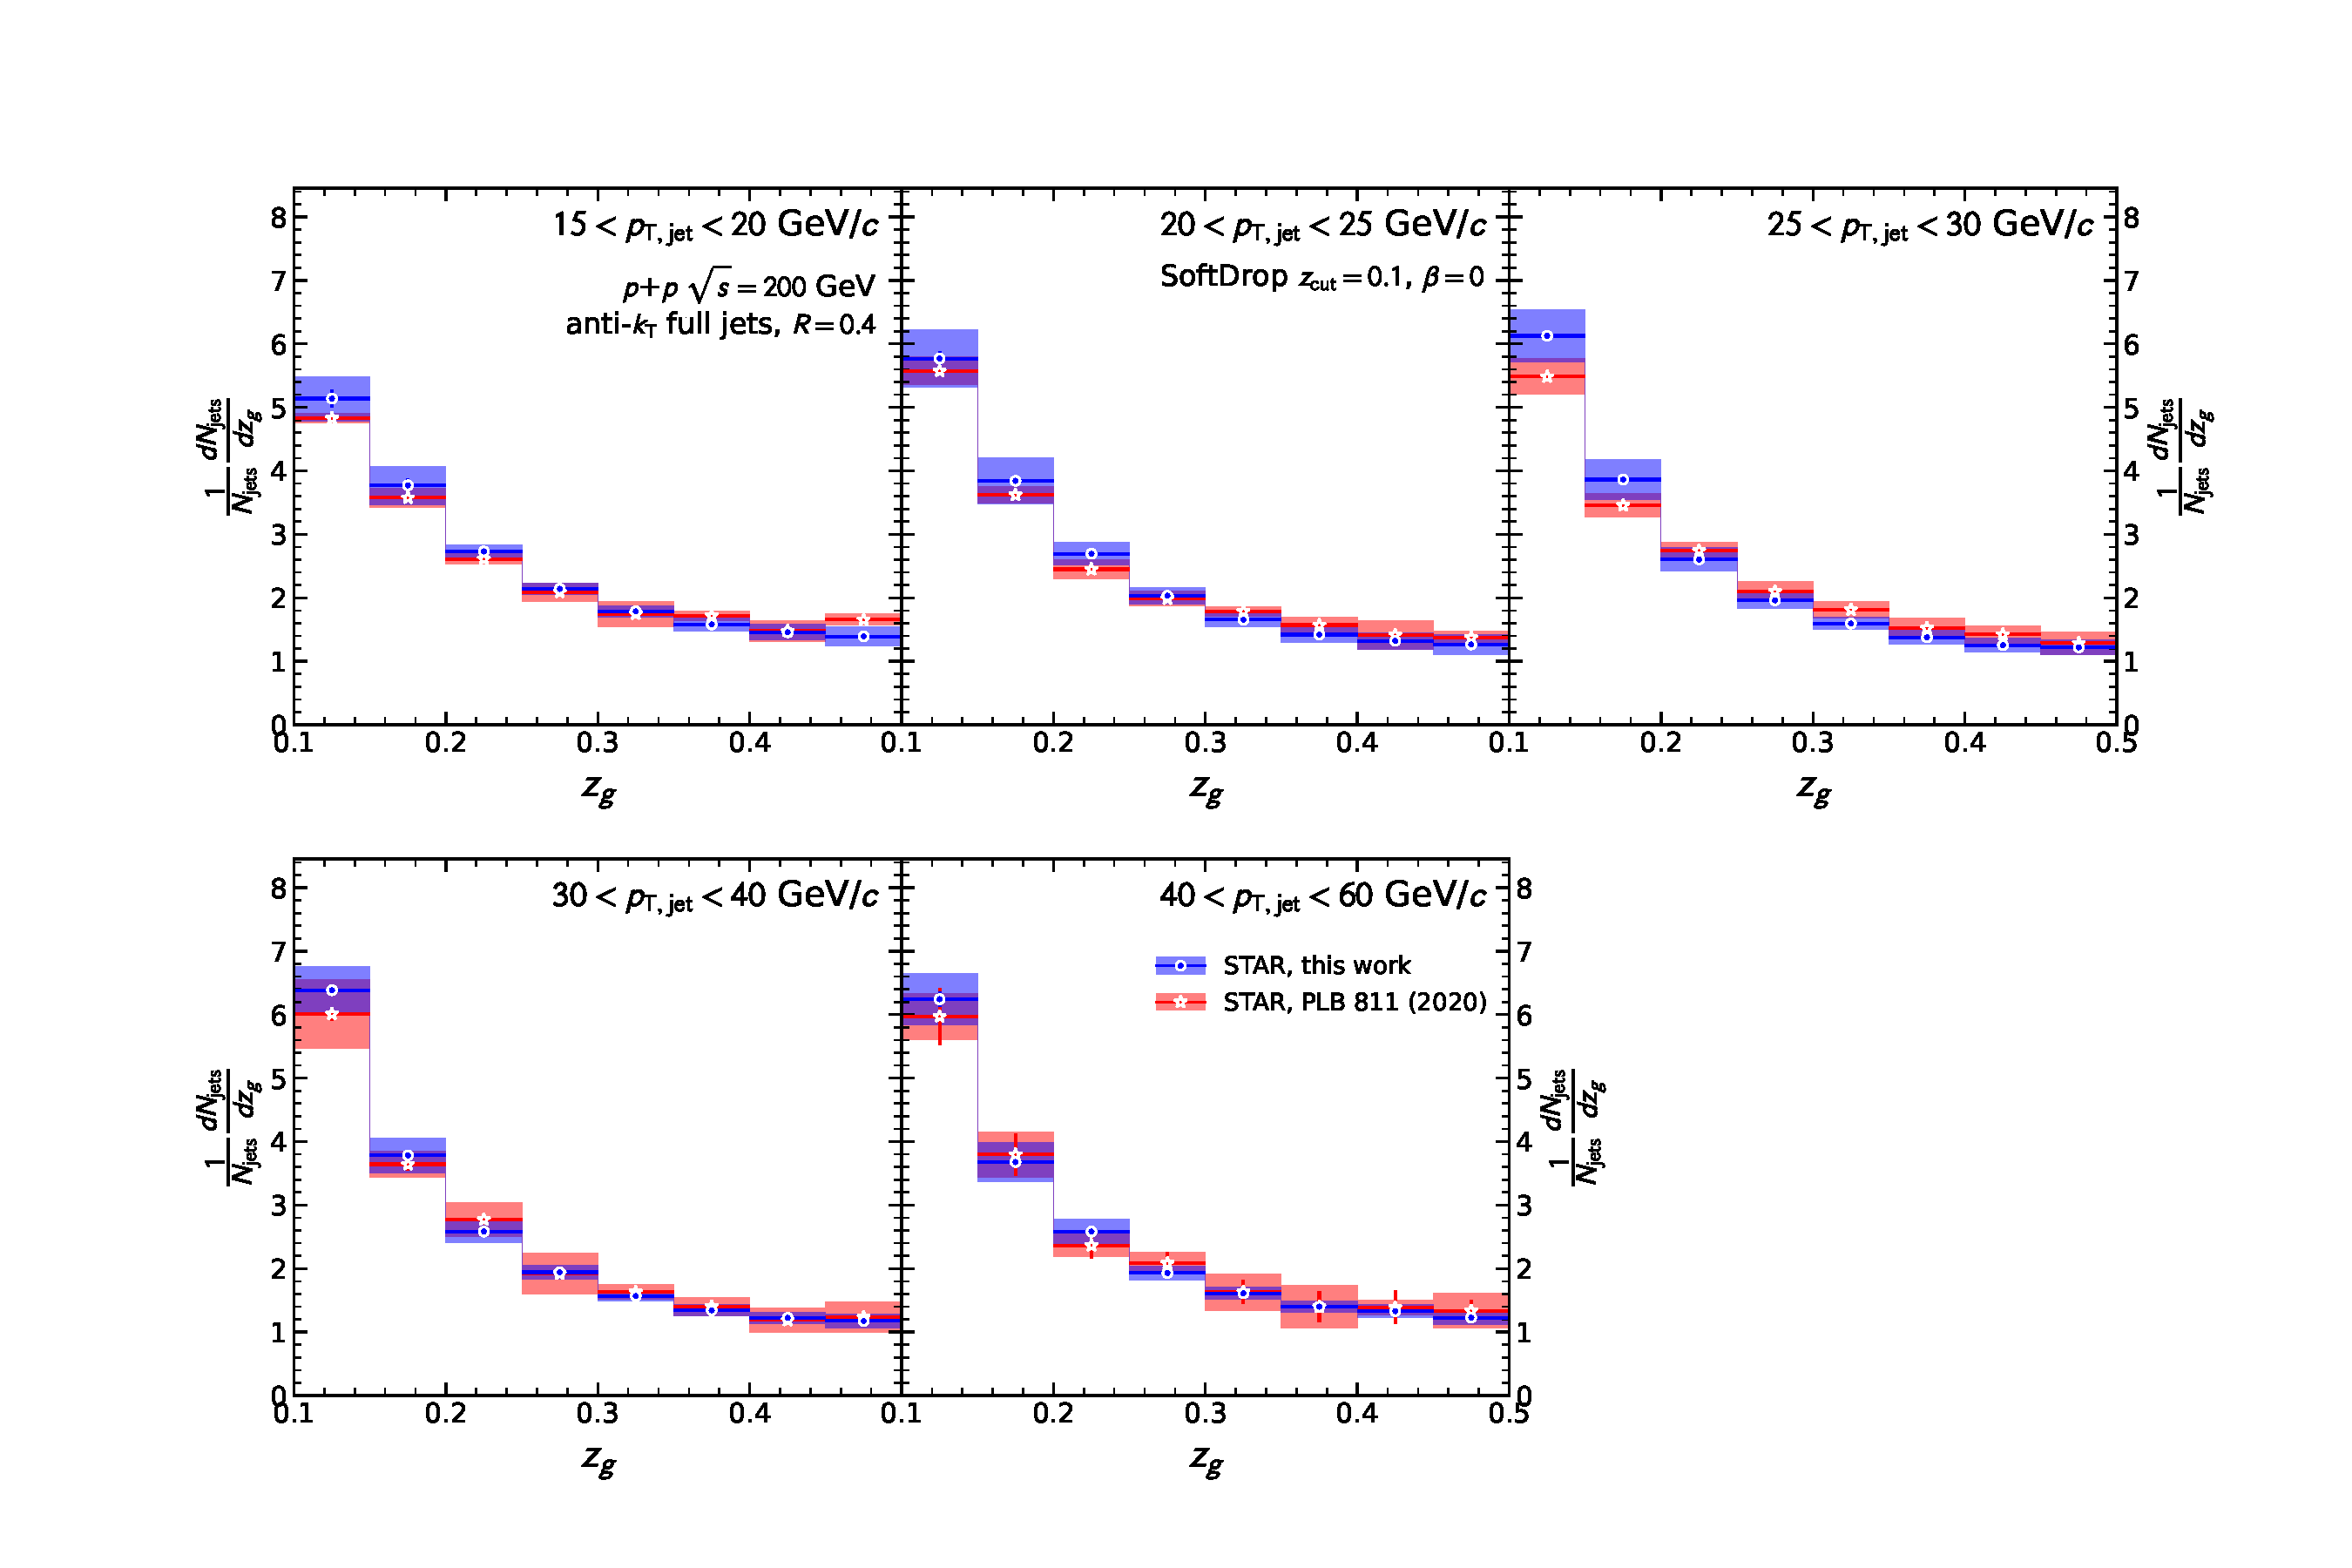
\includegraphics[width=0.495\linewidth]{angularities/pp/pub_comparison/star_published/star_pub_sd_symmetry}
	\begin{itemize}\setlength{\itemsep}{0pt}
		\scriptsize
		\item Same unfolded jets, \(z_\mathrm{cut} = 0.1\): \Rg, \zg \textbf{agree}
	\end{itemize}
	\refnote{STAR, PLB 811 (2020) 135846}
\end{frame}

\begin{frame}{Backup: published STAR jet mass}
	\centering
	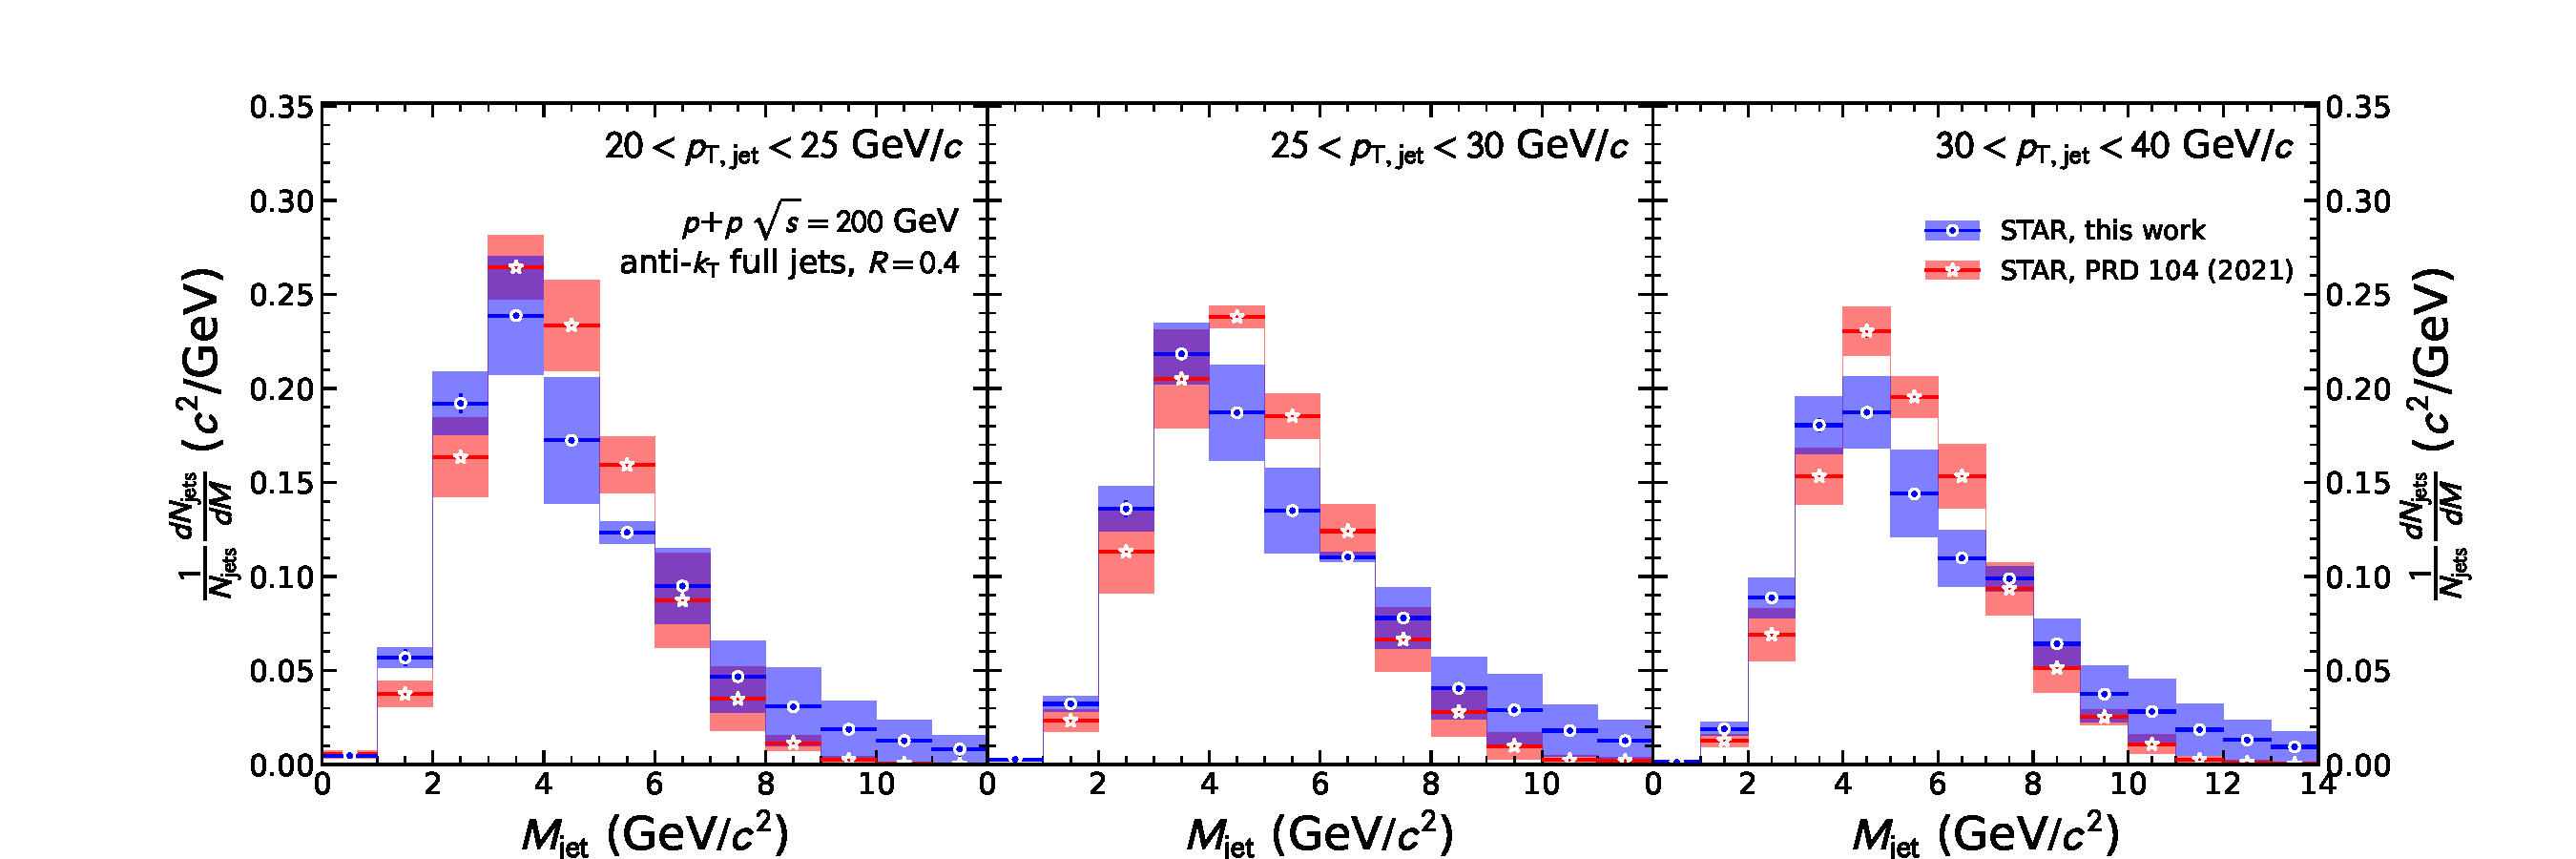
\includegraphics[width=0.495\linewidth]{angularities/pp/pub_comparison/star_published/star_pub_m}
	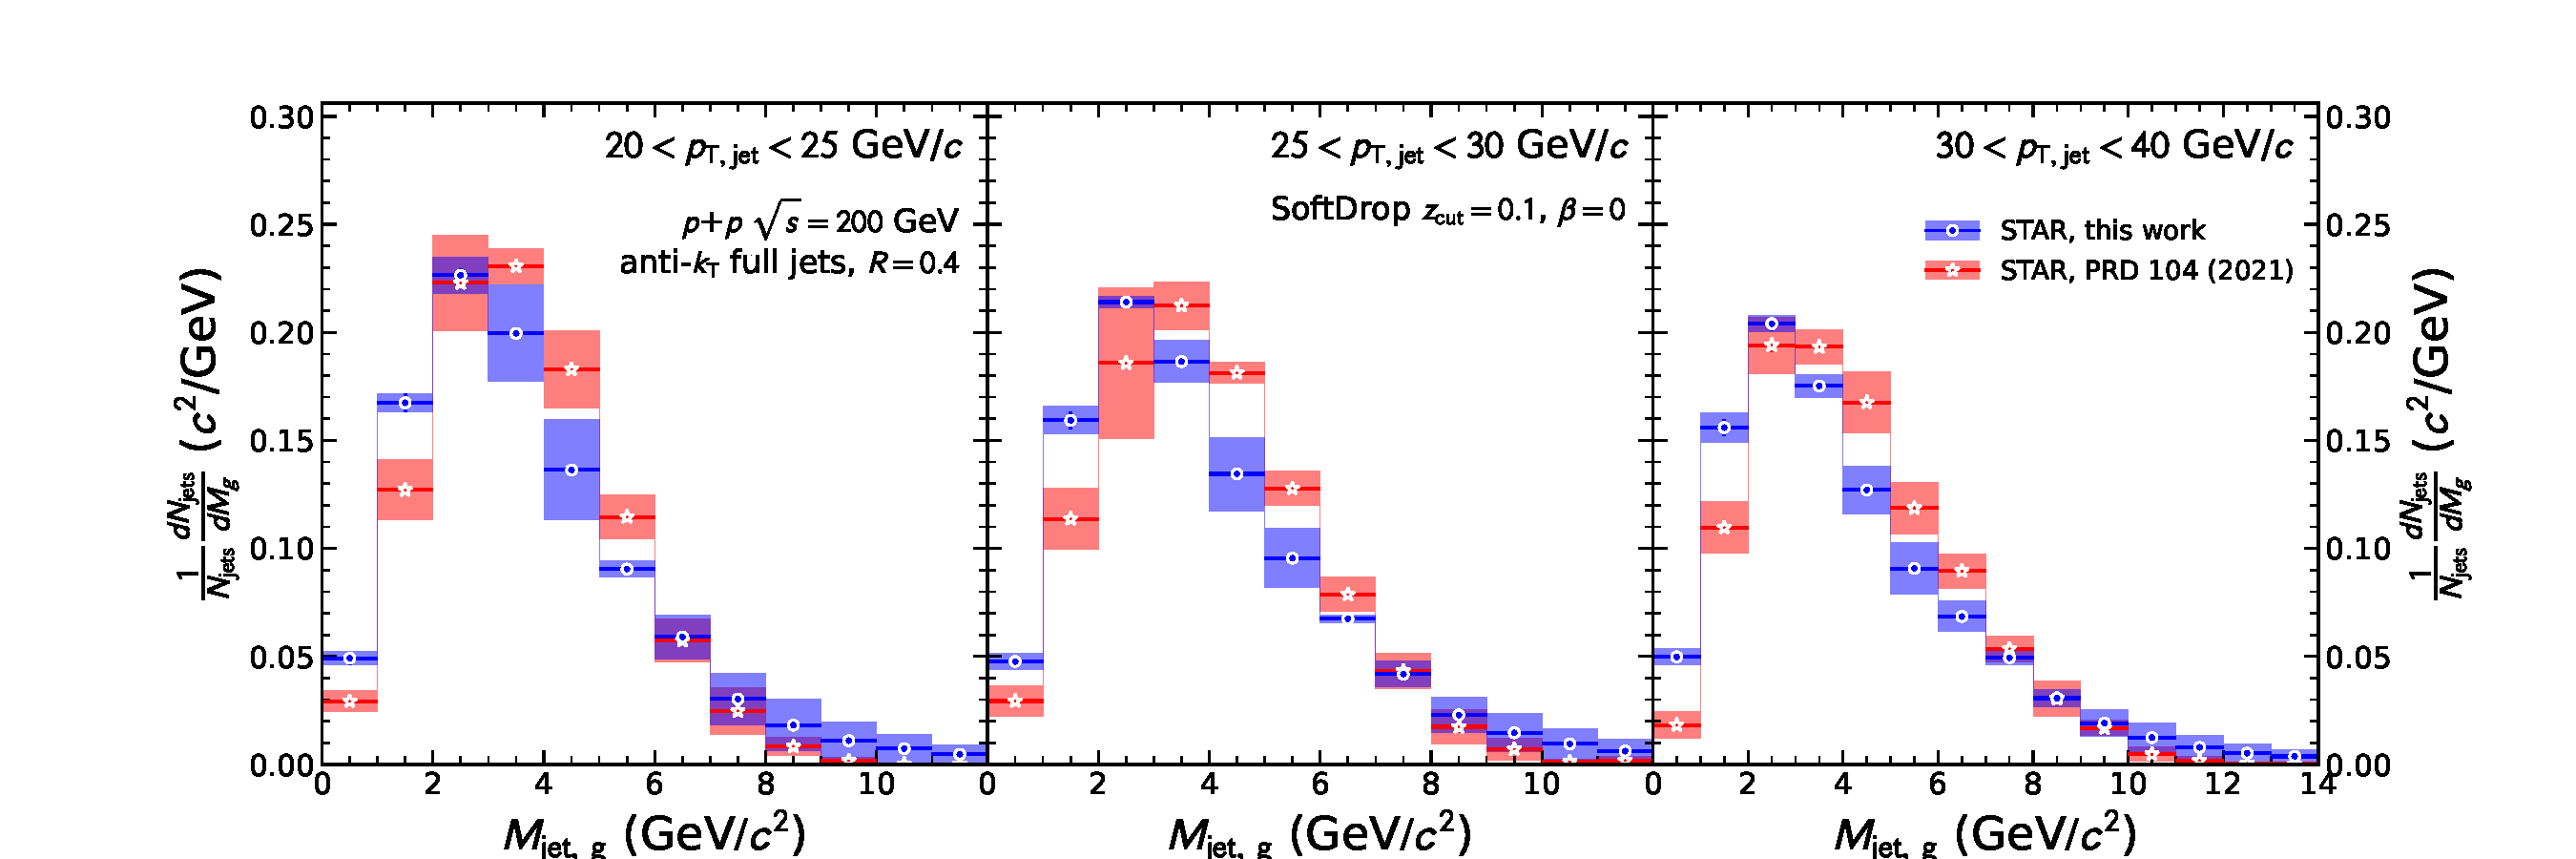
\includegraphics[width=0.495\linewidth]{angularities/pp/pub_comparison/star_published/star_pub_sd_m}
	\begin{itemize}\setlength{\itemsep}{0pt}
		\scriptsize
		\item \(M\), \(M_\mathrm{g}\) \textbf{broader} than published --- under investigation
	\end{itemize}
	\refnote{STAR, PRD 104 (2021) 052007}
\end{frame}

\begin{frame}{Backup: event-plane resolution}
	\begin{columns}[c]
		\begin{column}{0.59\textwidth}
			\centering
			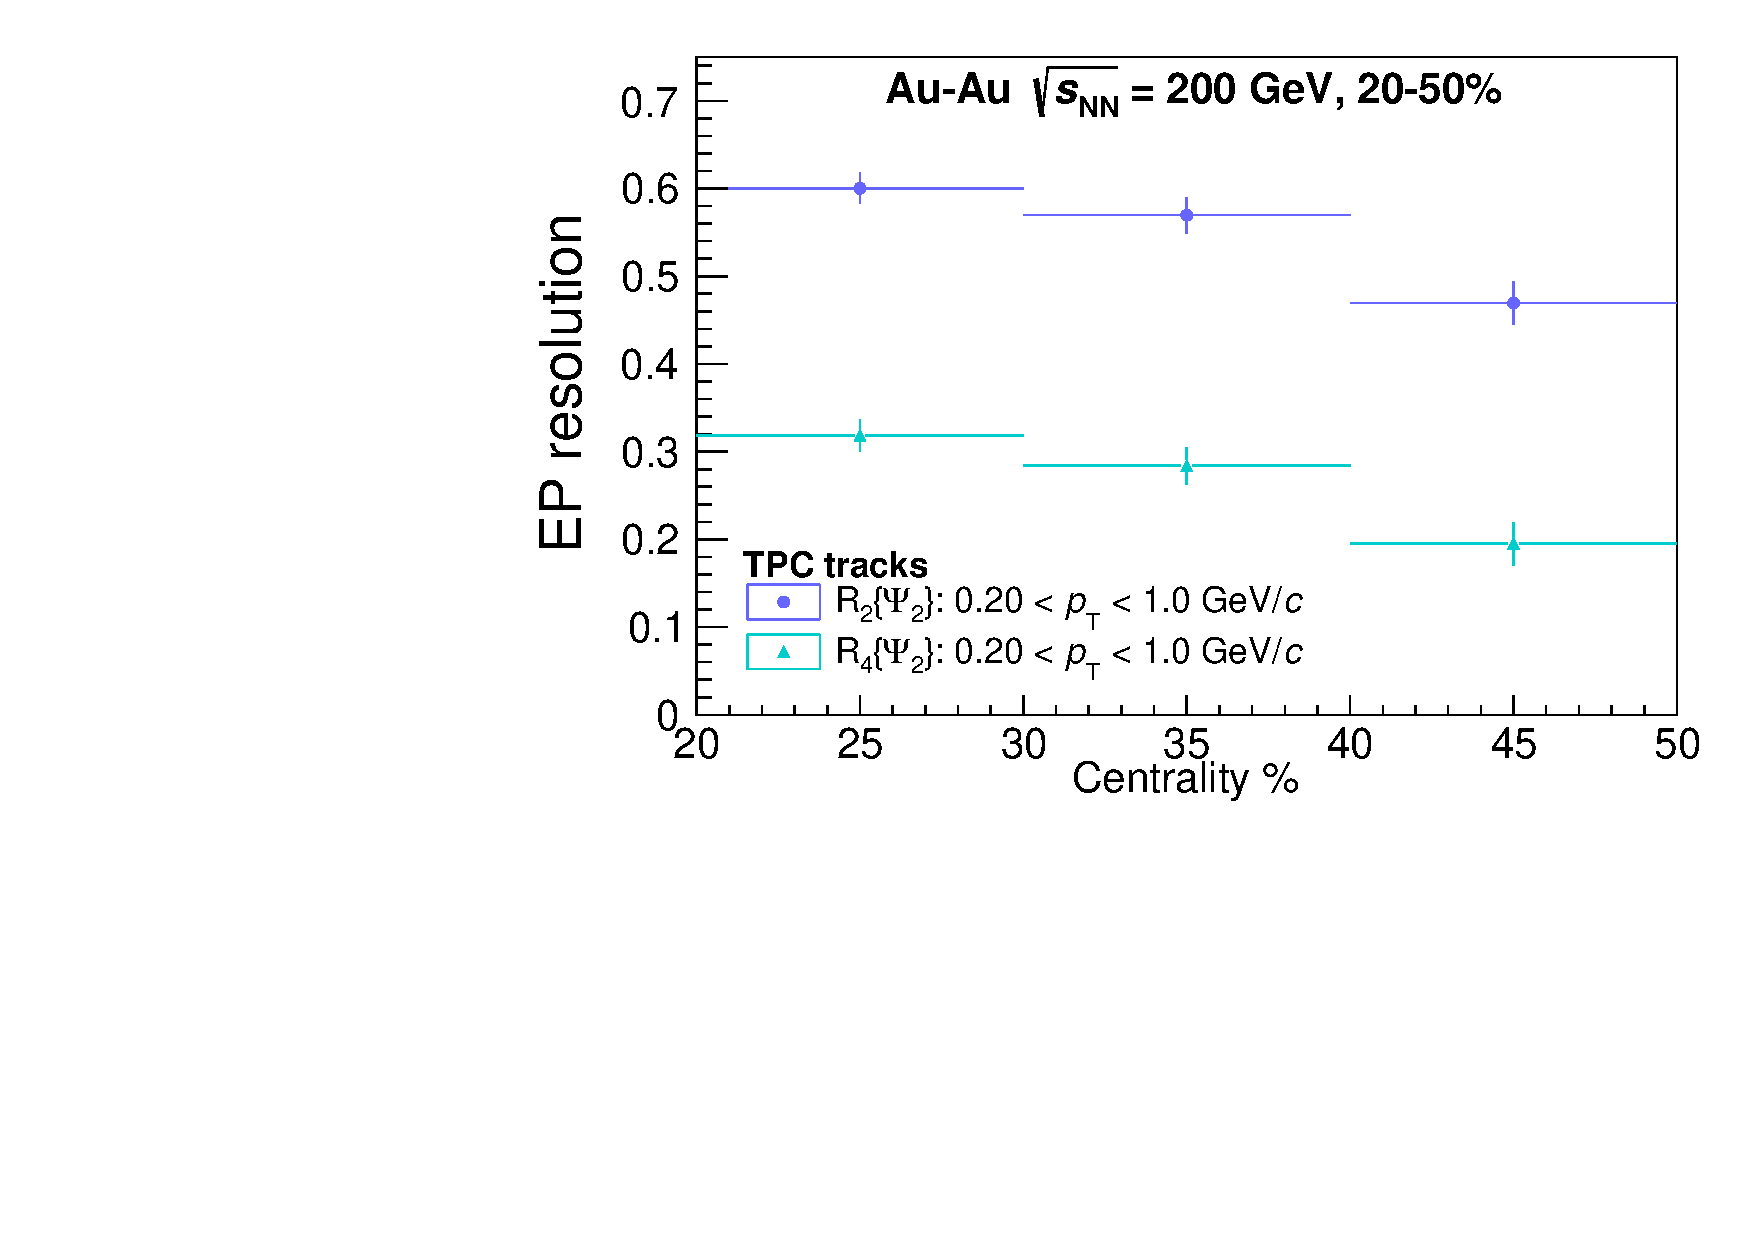
\includegraphics[width=\linewidth]{R2-4combined.pdf}
		\end{column}
		\begin{column}{0.39\textwidth}
			\begin{itemize}
				\item Background: \(R_n\) in RPF \(\Rightarrow\) corrected
				\item Signal: not corrected; \(v_2^\mathrm{quench} \to R_2 v_2^\mathrm{quench}\)
			\end{itemize}
		\end{column}
	\end{columns}
\end{frame}

\begin{frame}{Backup: reaction plane fit (RPF)}
	\centering
	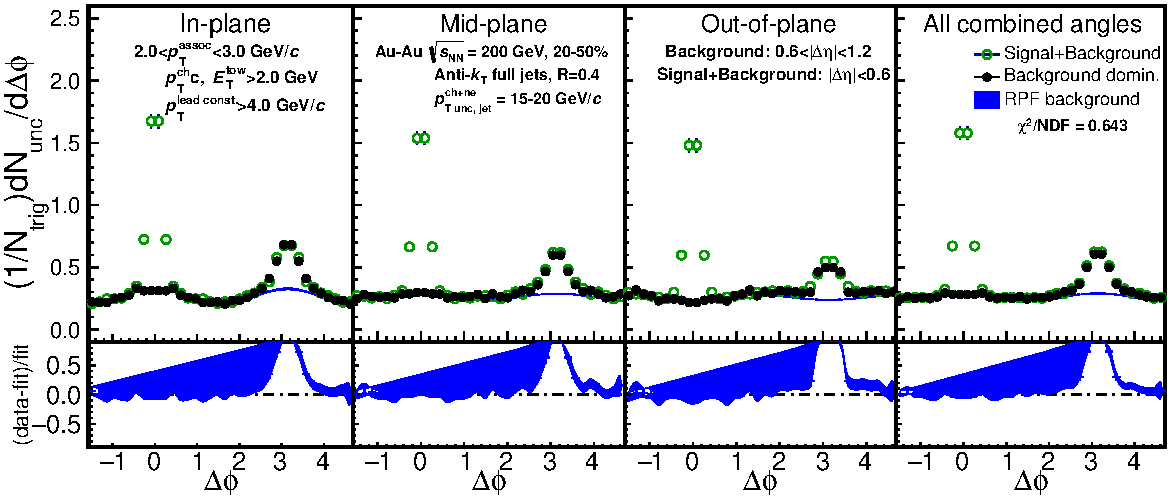
\includegraphics[width=\linewidth,height=0.6\textheight,keepaspectratio]{JHC/JHCorrBGsub_A2.0-3.0_T15-20_C20-50.pdf}
	\begin{itemize}\setlength{\itemsep}{0pt}
		\small
		\item Flow background: \textbf{reaction plane fit} (RPF), all orientations at once
		\item EP resolution \(R_2 = 0.56\) \(\Rightarrow\) true in/out difference halved
	\end{itemize}
	\refnote{STAR, PRC 109 (2024) 044909}
\end{frame}

\begin{frame}{Backup: RPF fit parameters}
	\centering
	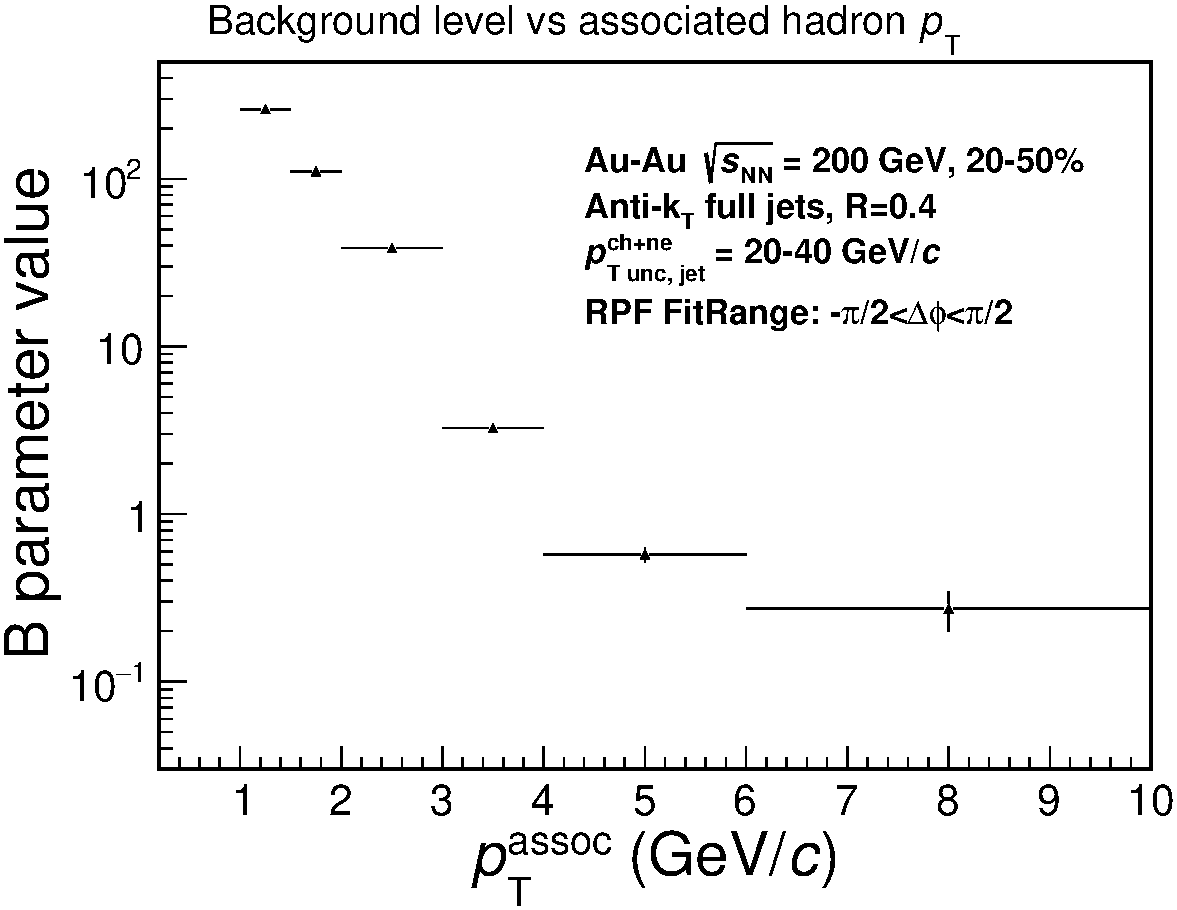
\includegraphics[width=0.45\linewidth]{JHC/FitPars_Background_J20-40_C20-50_Zcut24.pdf}
	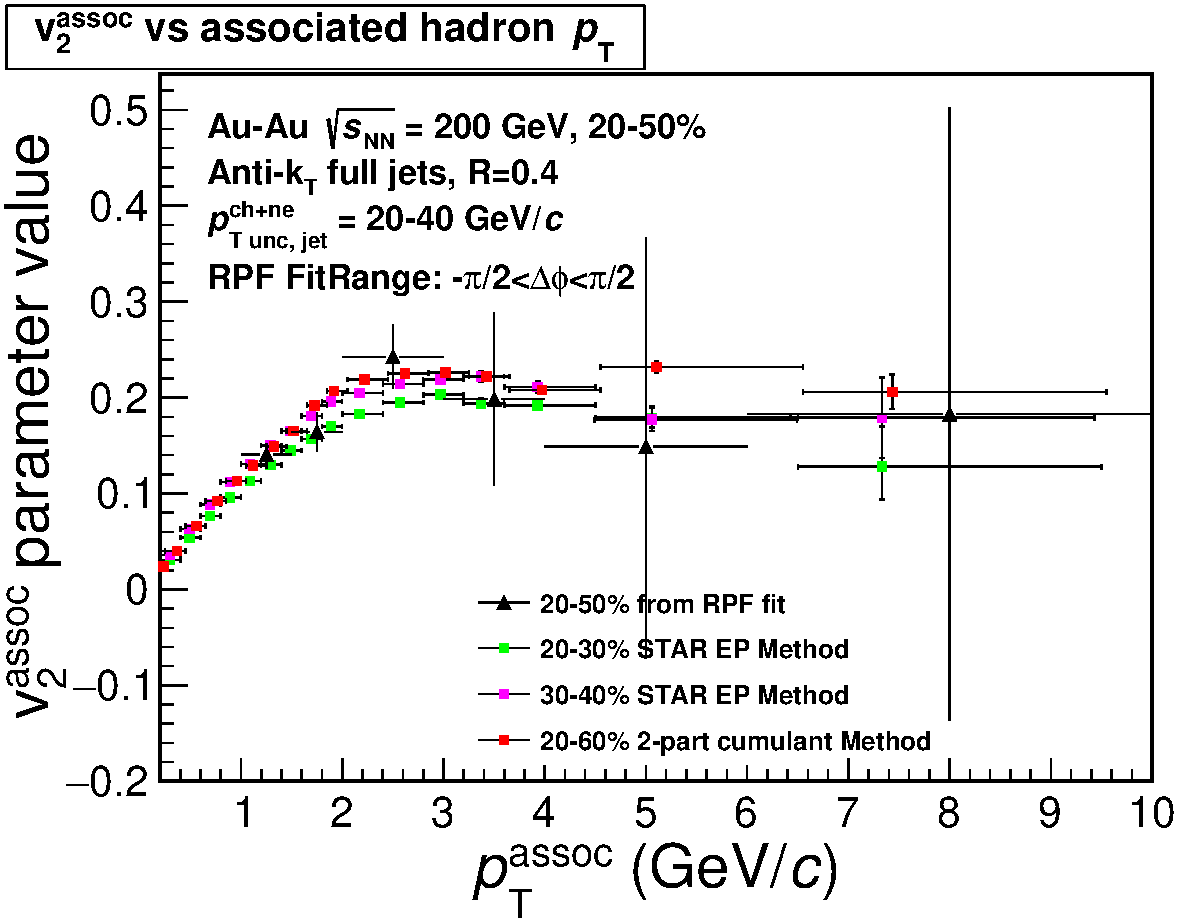
\includegraphics[width=0.45\linewidth]{JHC/FitPars_v2Assoc_J20-40_C20-50_Zcut24.pdf}
\end{frame}

\begin{frame}{Backup: jet-hadron yields and ratios, 15--20~GeV/\(c\) jets}
	\centering
	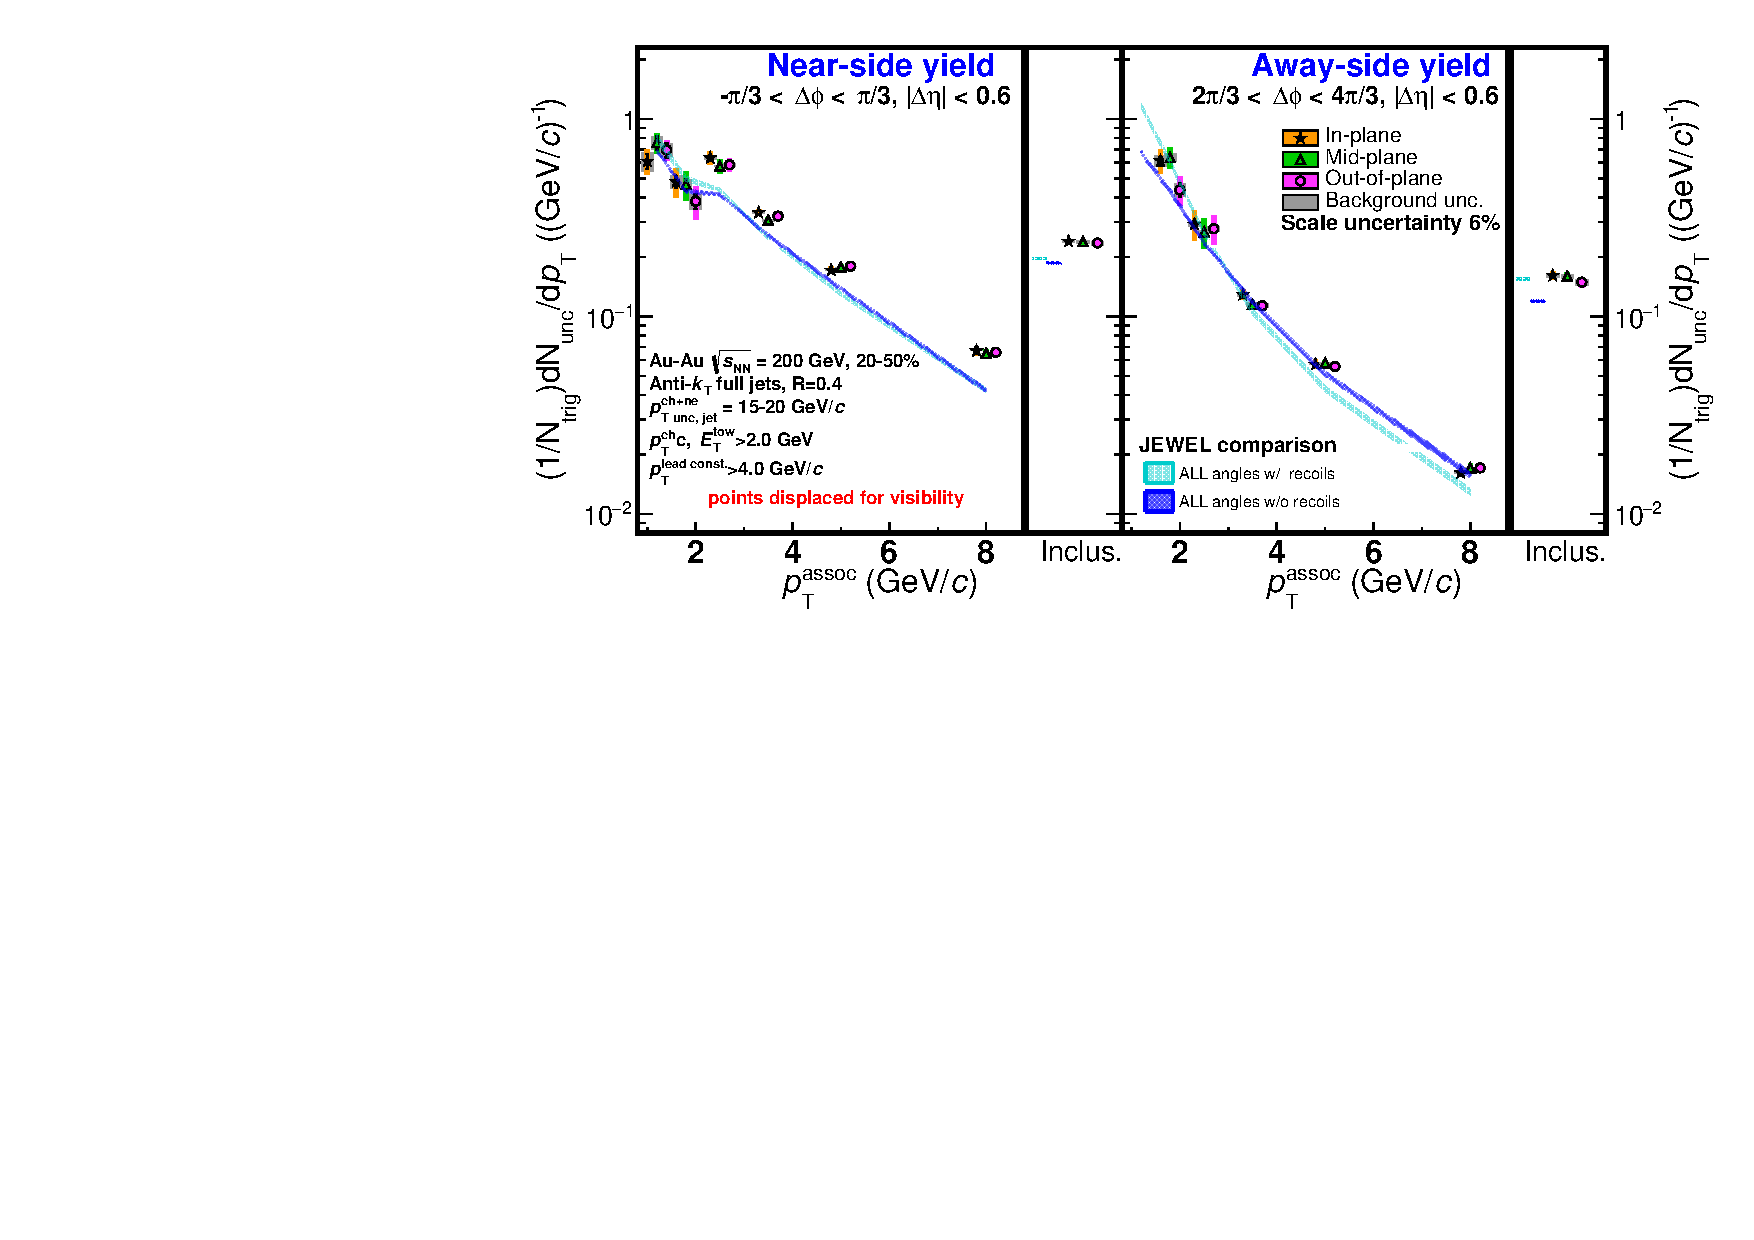
\includegraphics[width=0.49\linewidth]{JHC/results/NearAwaySideYield_J15-20_C20-50_wJEScorr_wJEWELerr.pdf}
	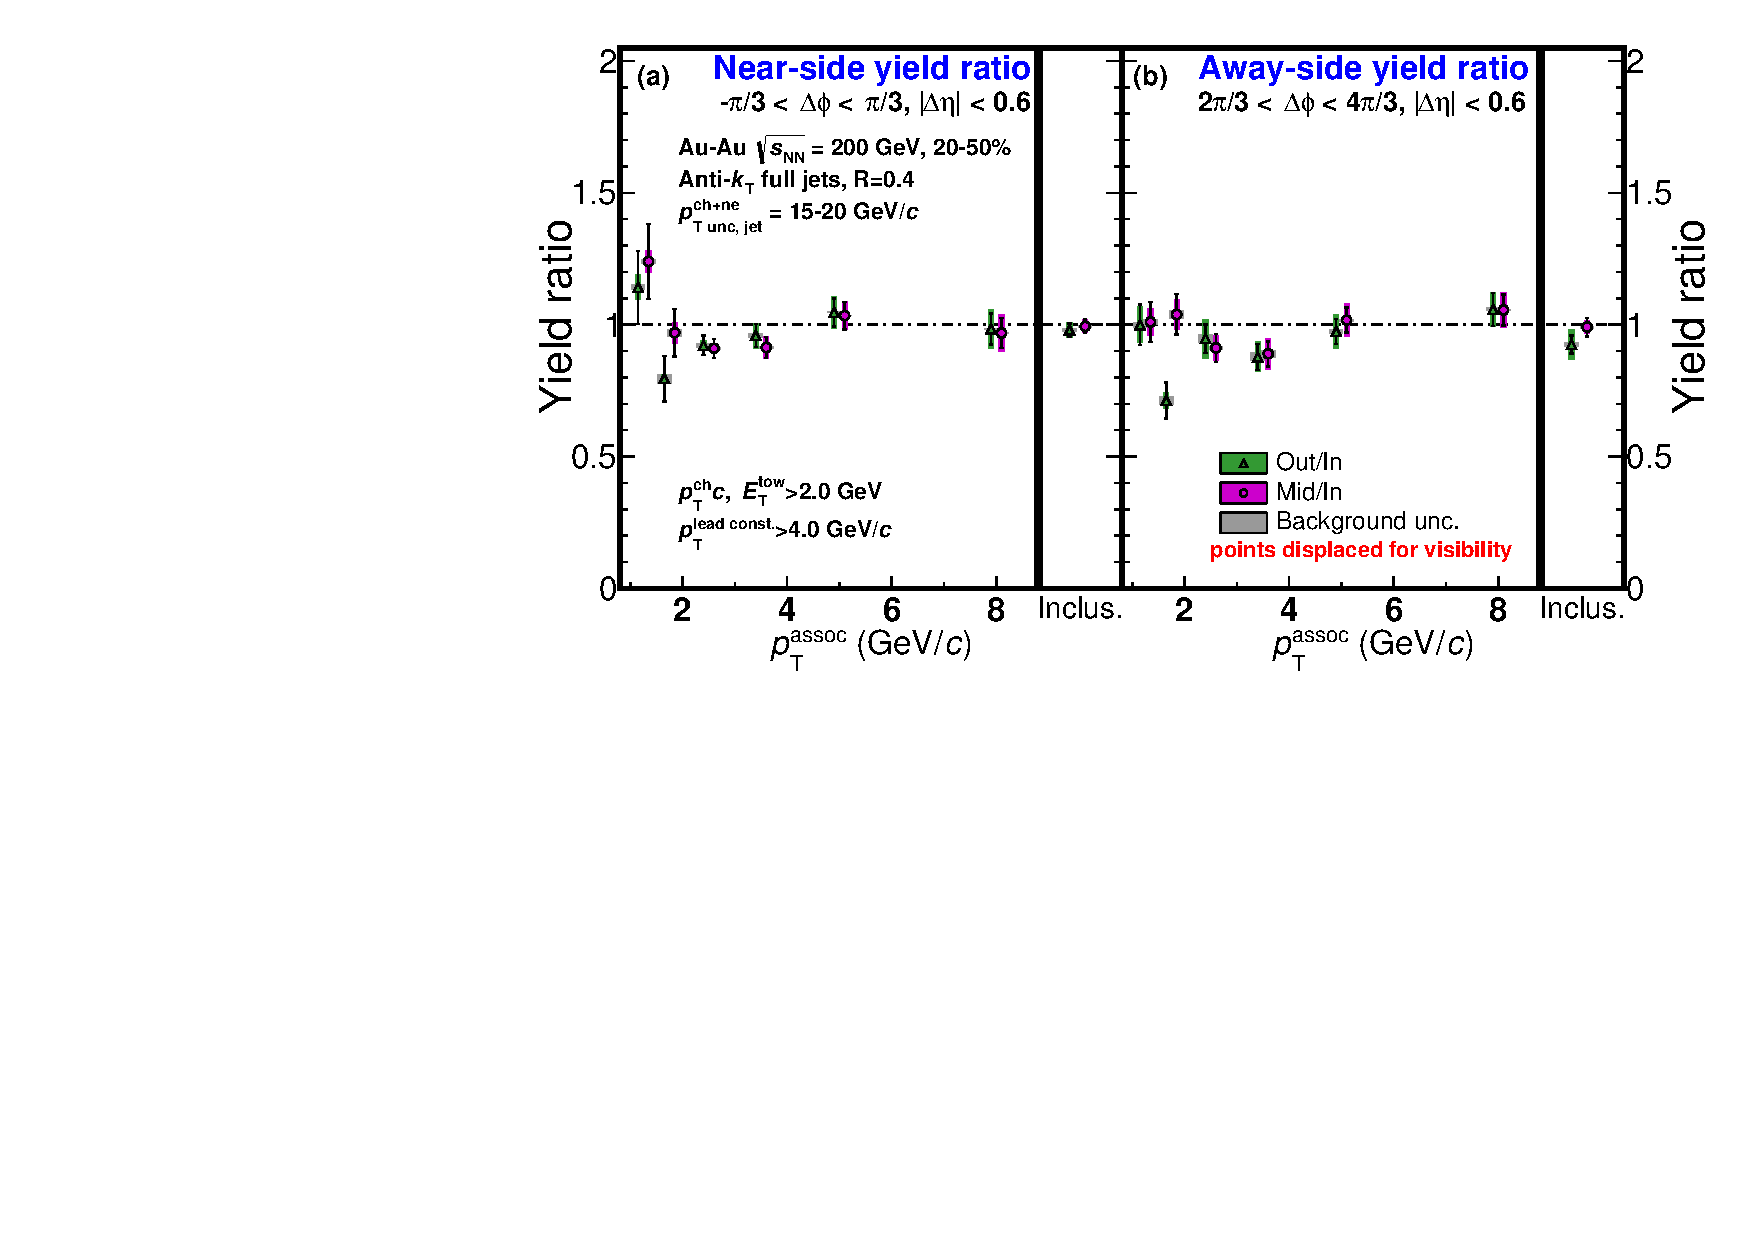
\includegraphics[width=0.49\linewidth]{JHC/results/YieldRatio_J15-20_C20-50_wJEScorr.pdf}
\end{frame}

\begin{frame}{Backup: jet-peak widths}
	\centering
	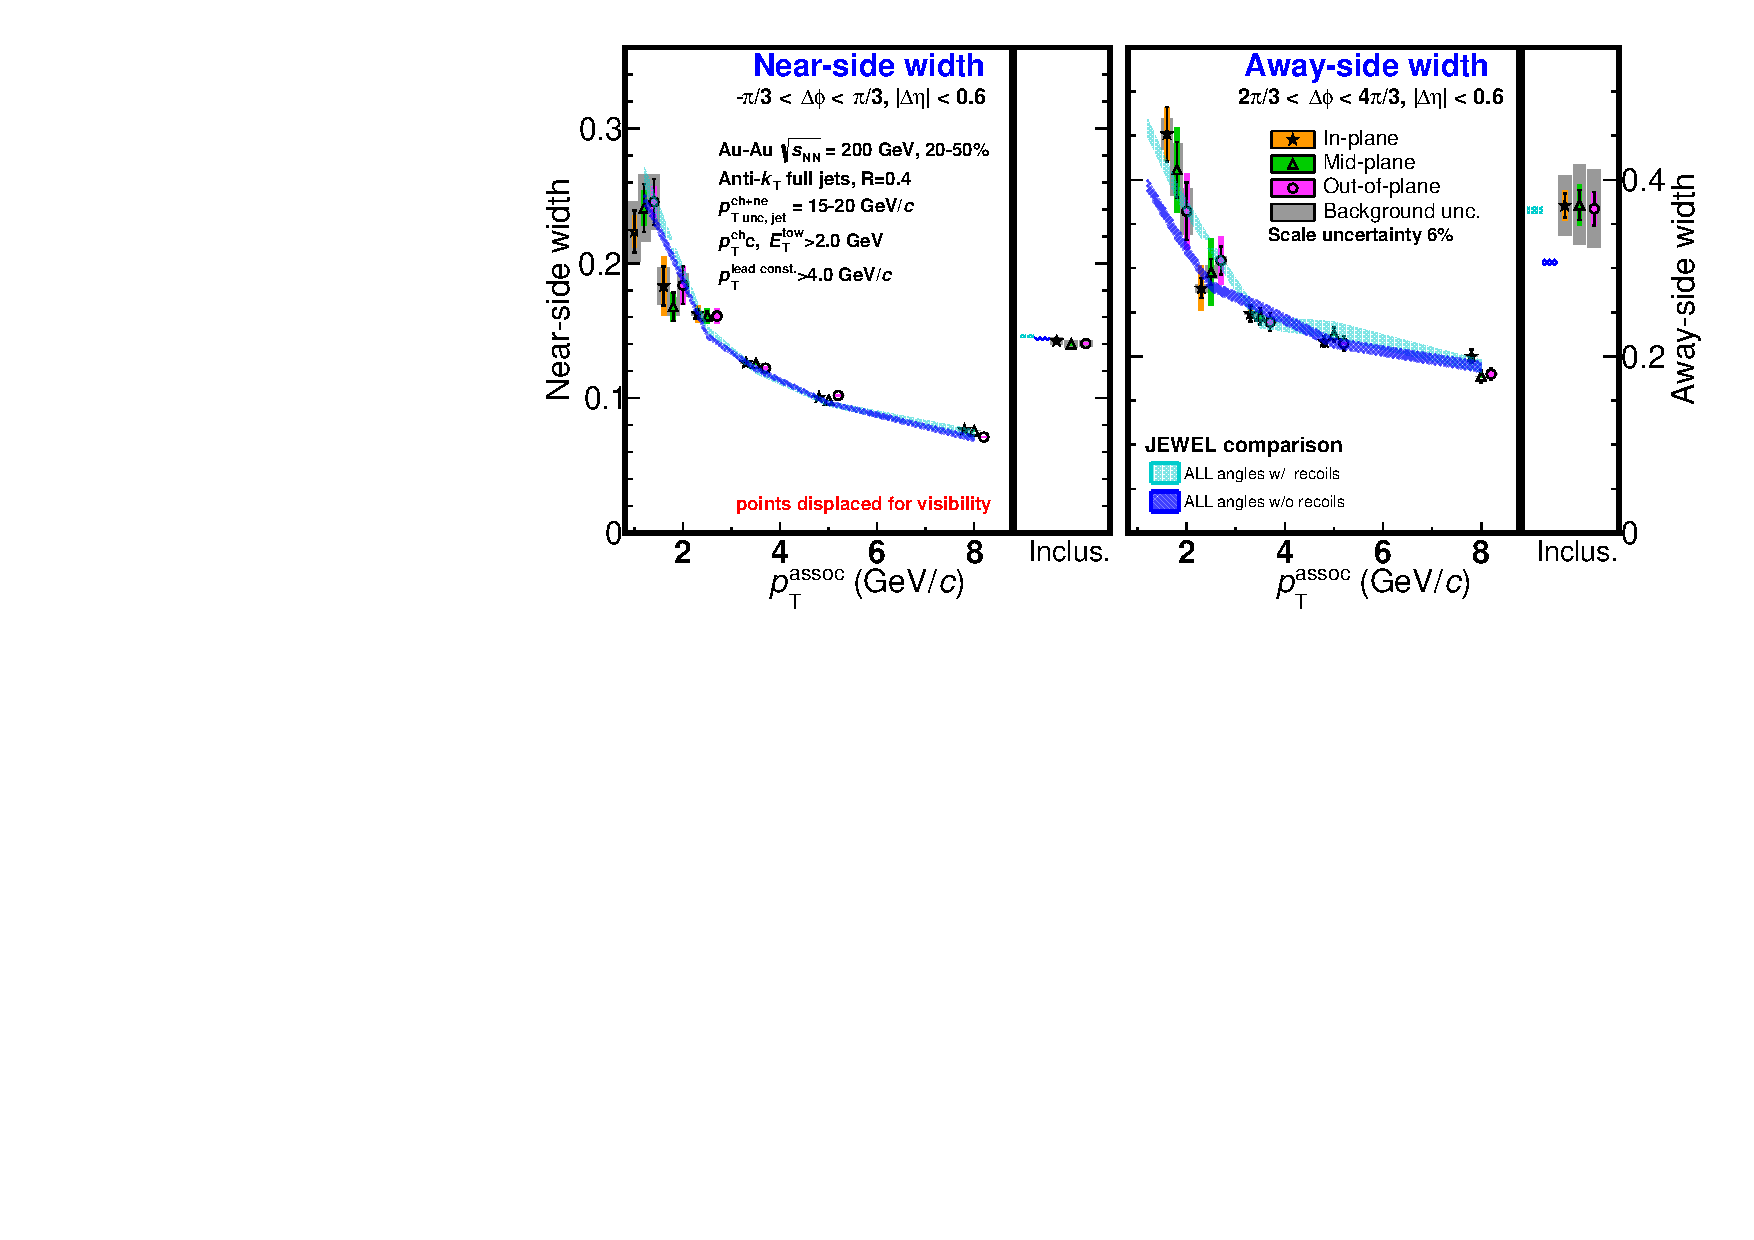
\includegraphics[width=0.49\linewidth]{JHC/results/NearAwaySideWidths_J15-20_C20-50_wJEScorr_wJEWELerr.pdf}
	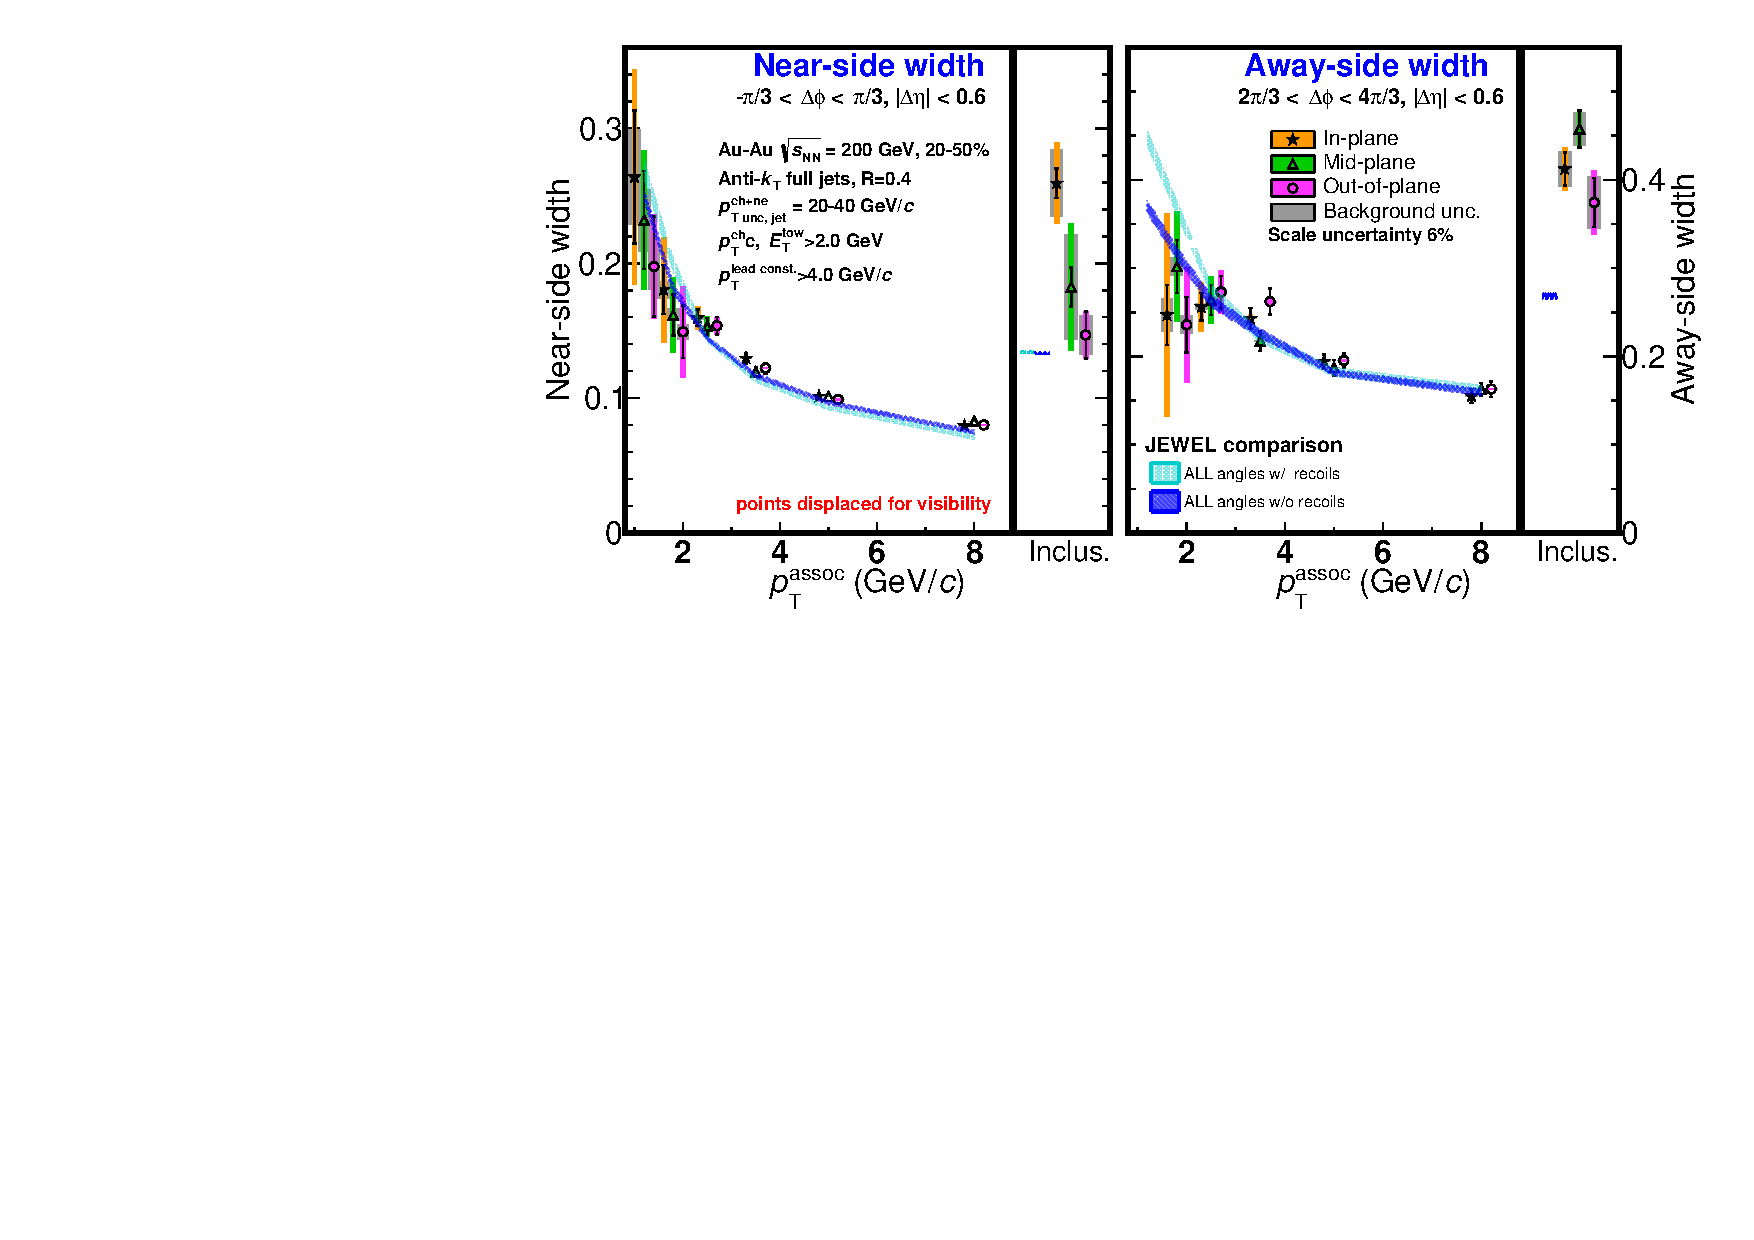
\includegraphics[width=0.49\linewidth]{JHC/results/NearAwaySideWidths_J20-40_C20-50_wJEScorr_wJEWELerr.pdf}
\end{frame}

\begin{frame}{Backup: Au+Au closure and systematics}
	\centering
	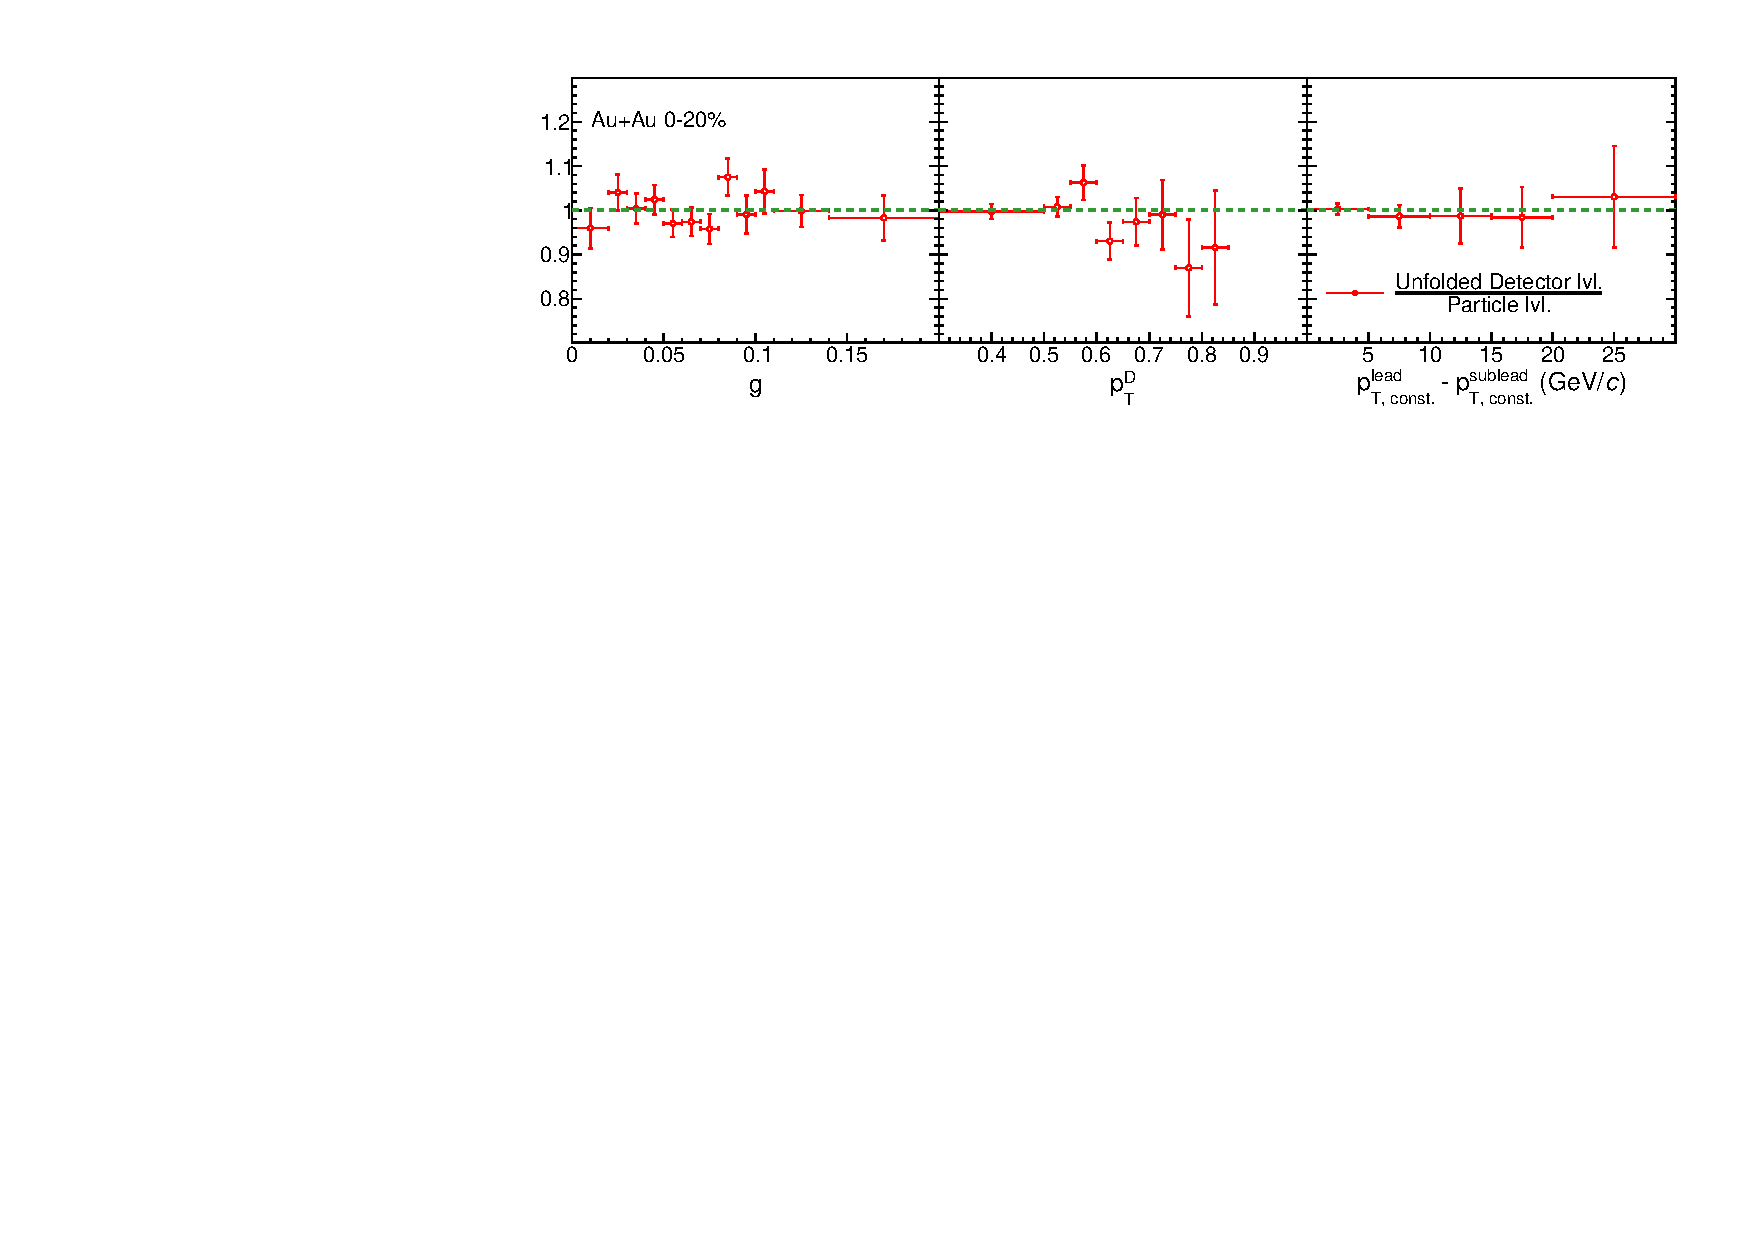
\includegraphics[width=0.7\linewidth]{angularities/AuAu/closure_cent0to20_v3}\\
	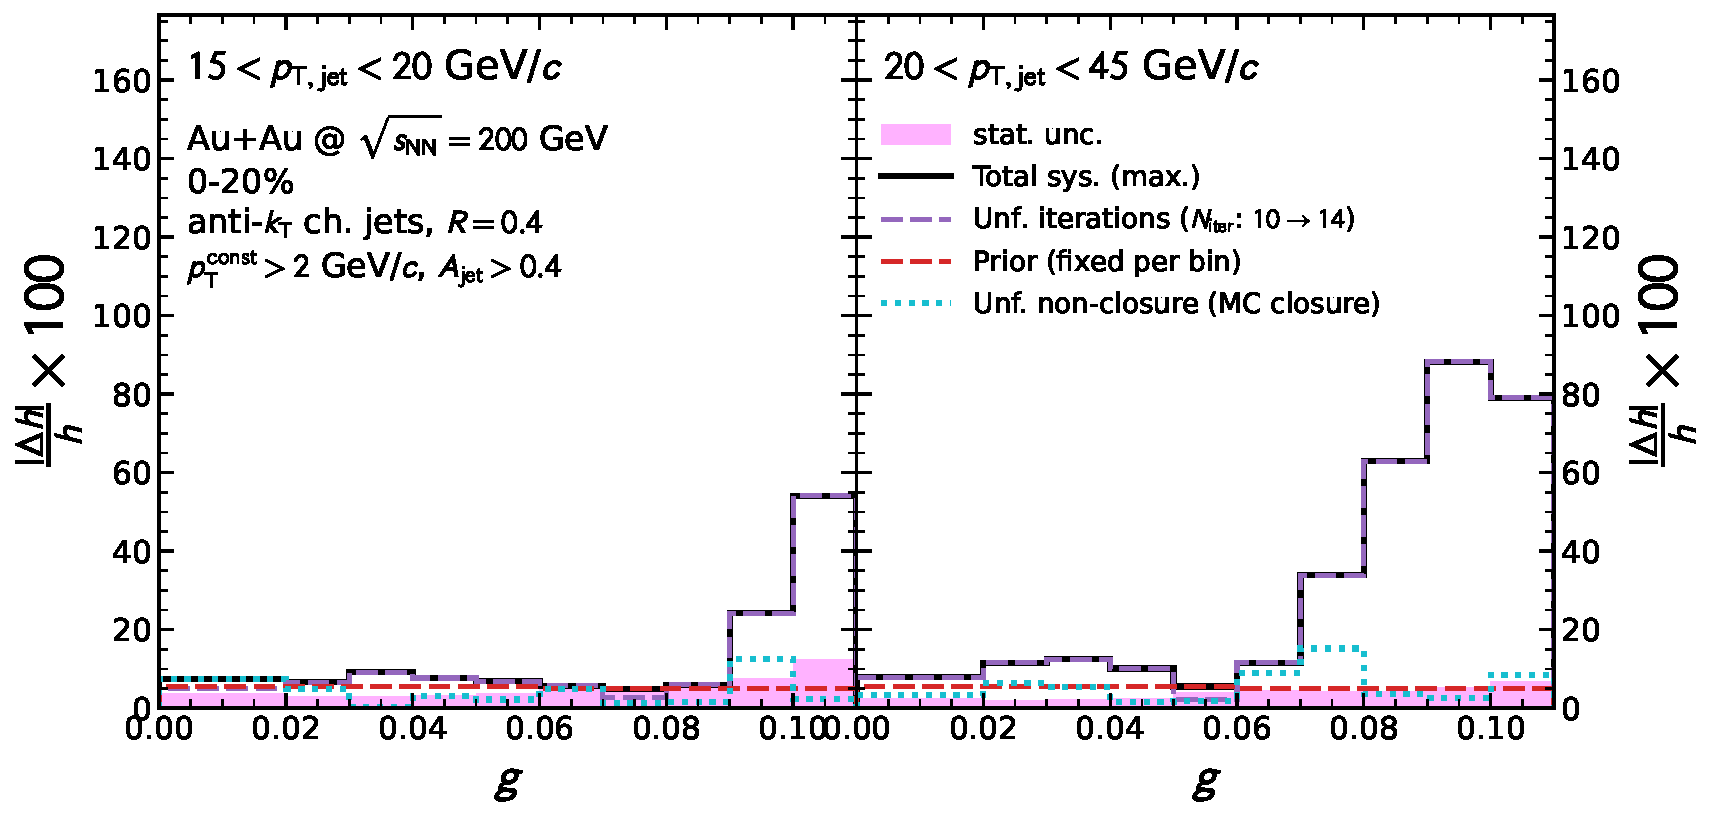
\includegraphics[width=0.3\linewidth]{angularities/AuAu/auau_sys_Girth_cent0to20.pdf}
	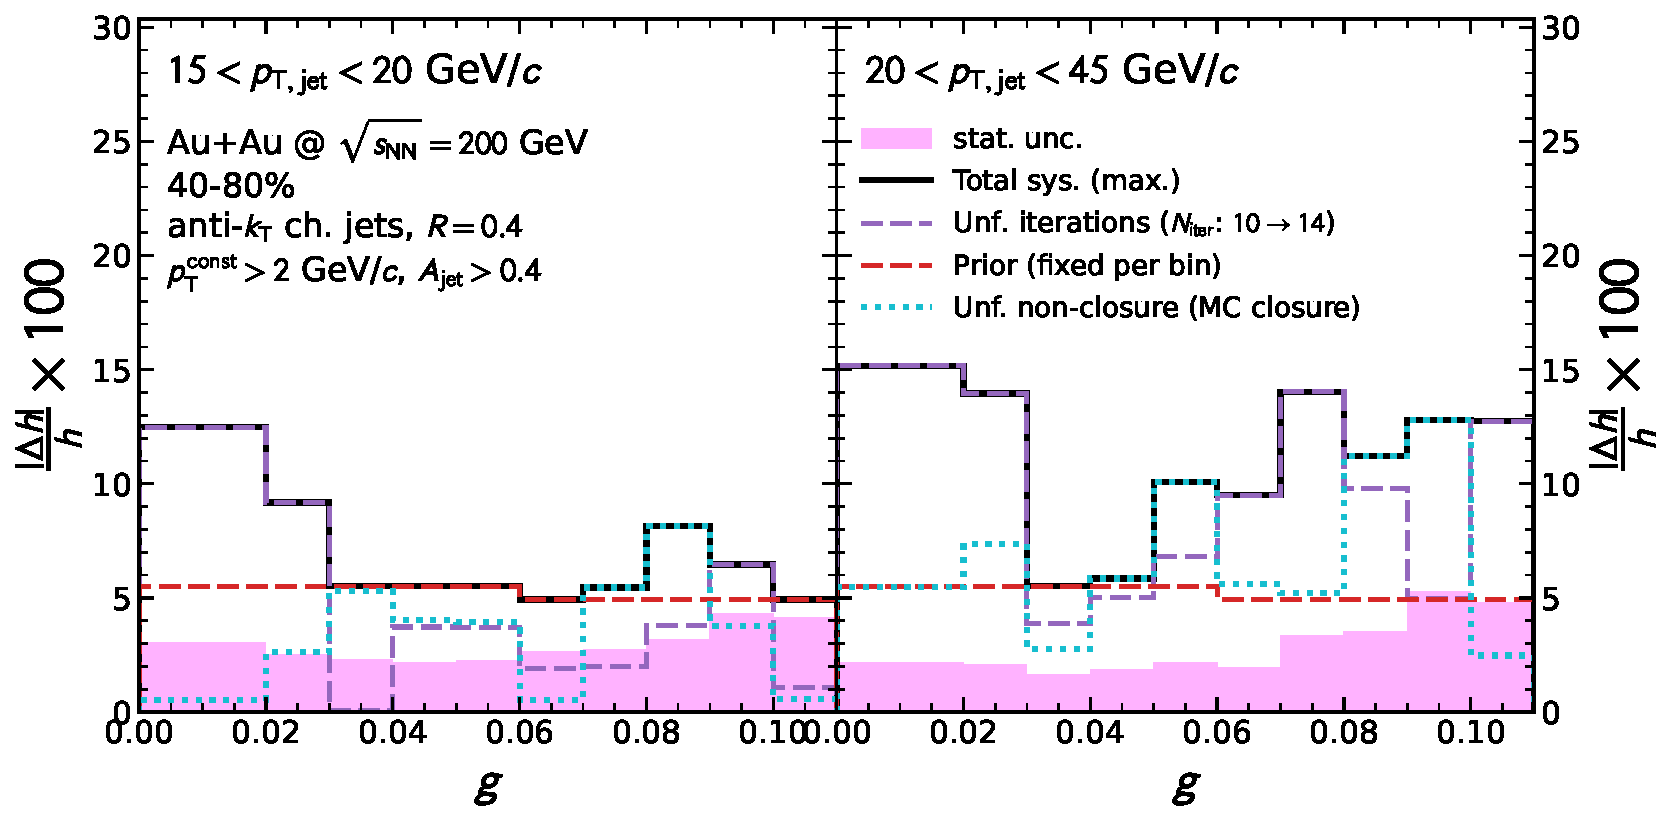
\includegraphics[width=0.3\linewidth]{angularities/AuAu/auau_sys_Girth_cent40to80.pdf}
	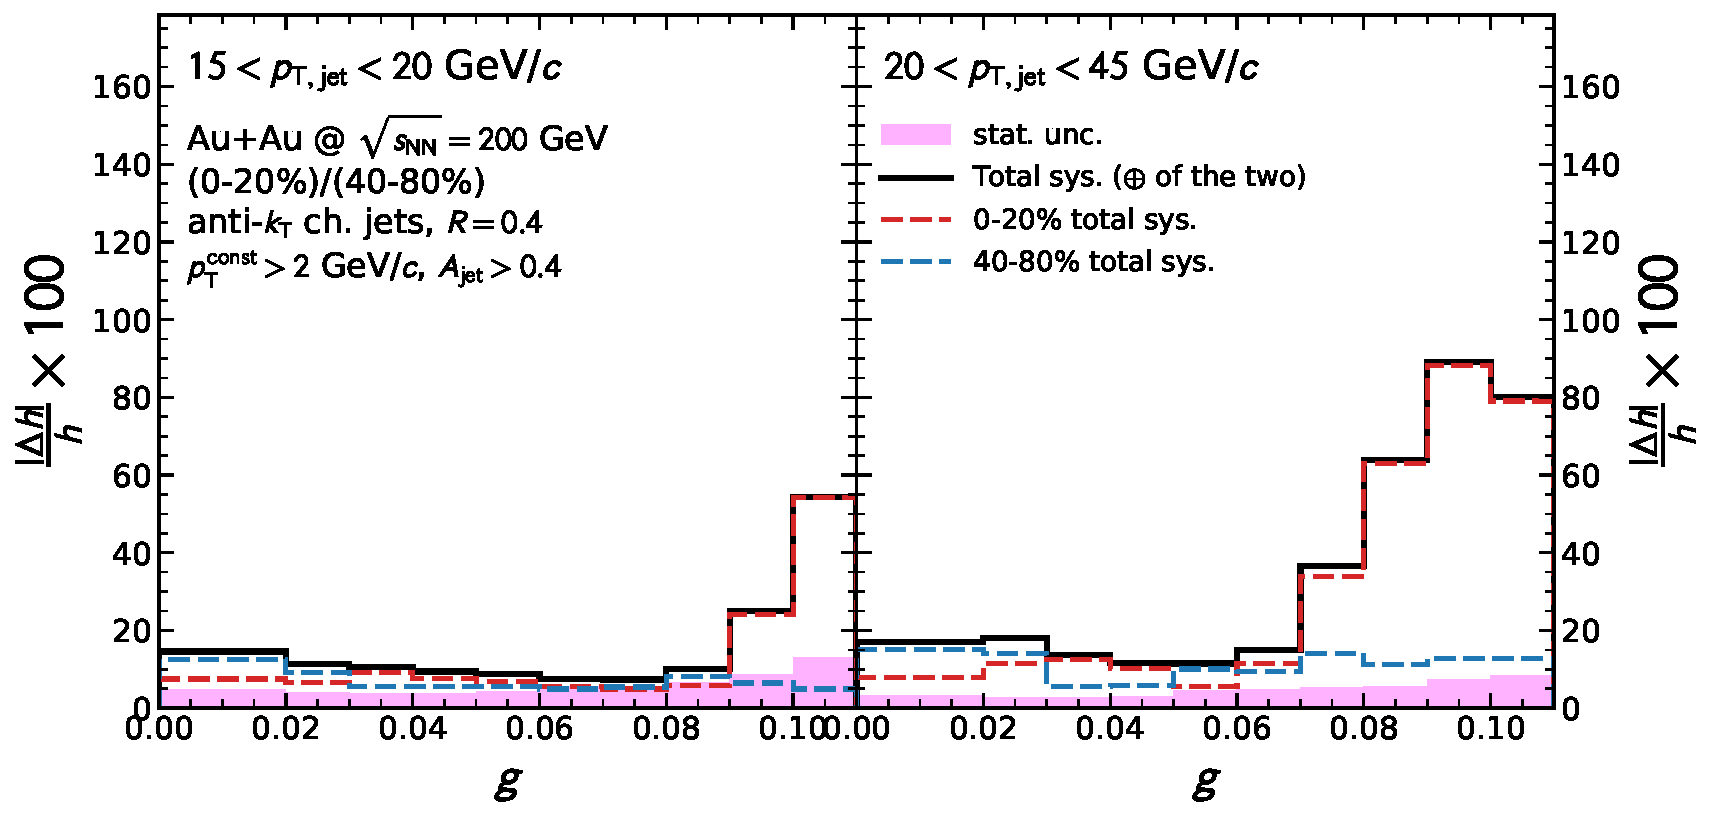
\includegraphics[width=0.3\linewidth]{angularities/AuAu/auau_sys_Girth_ratio.pdf}
\end{frame}

\begin{frame}{Backup: Au+Au results, 15--20~GeV/\(c\)}
	\centering
	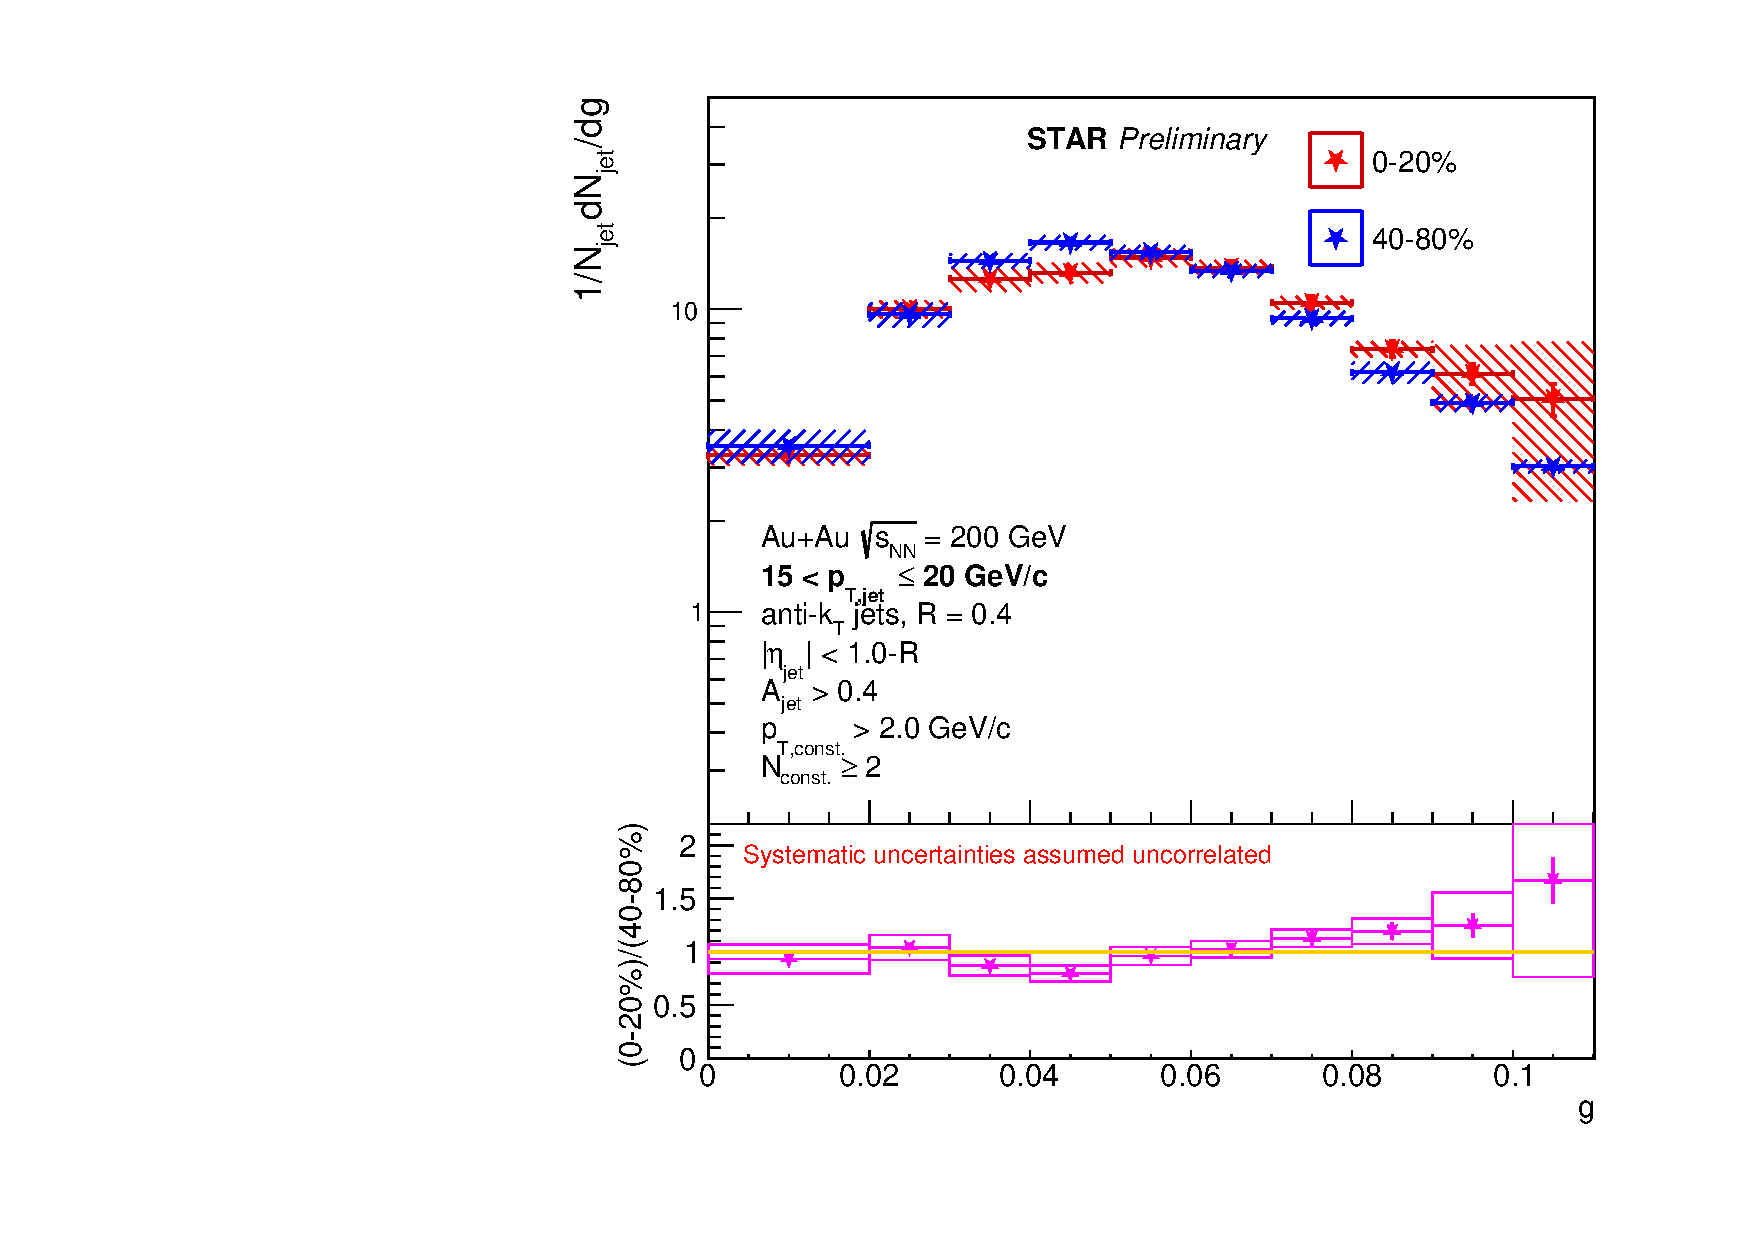
\includegraphics[width=0.32\linewidth]{angularities/AuAu/finalPlots_noPP_Girth_0_v3_warn.pdf}
	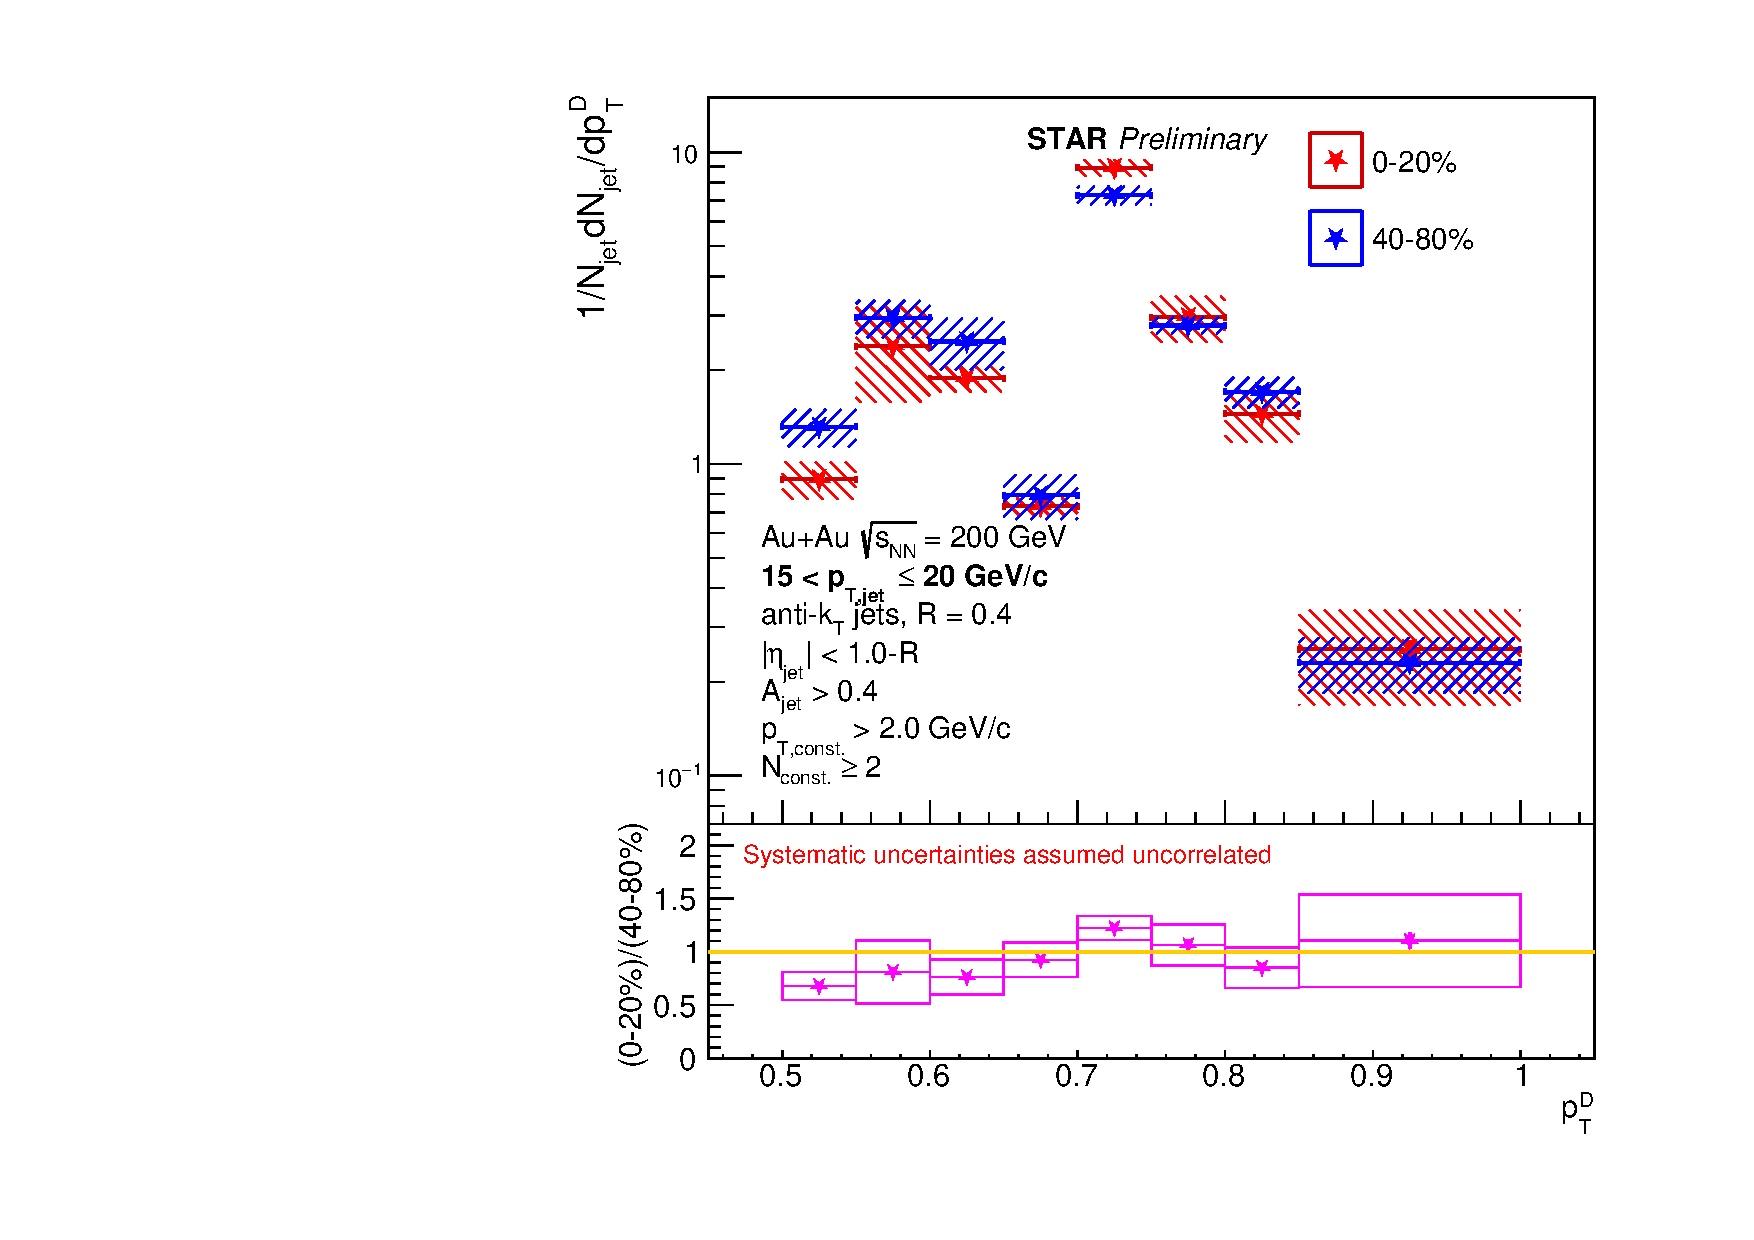
\includegraphics[width=0.32\linewidth]{angularities/AuAu/finalPlots_noPP_PtD_0_v3_warn.pdf}
	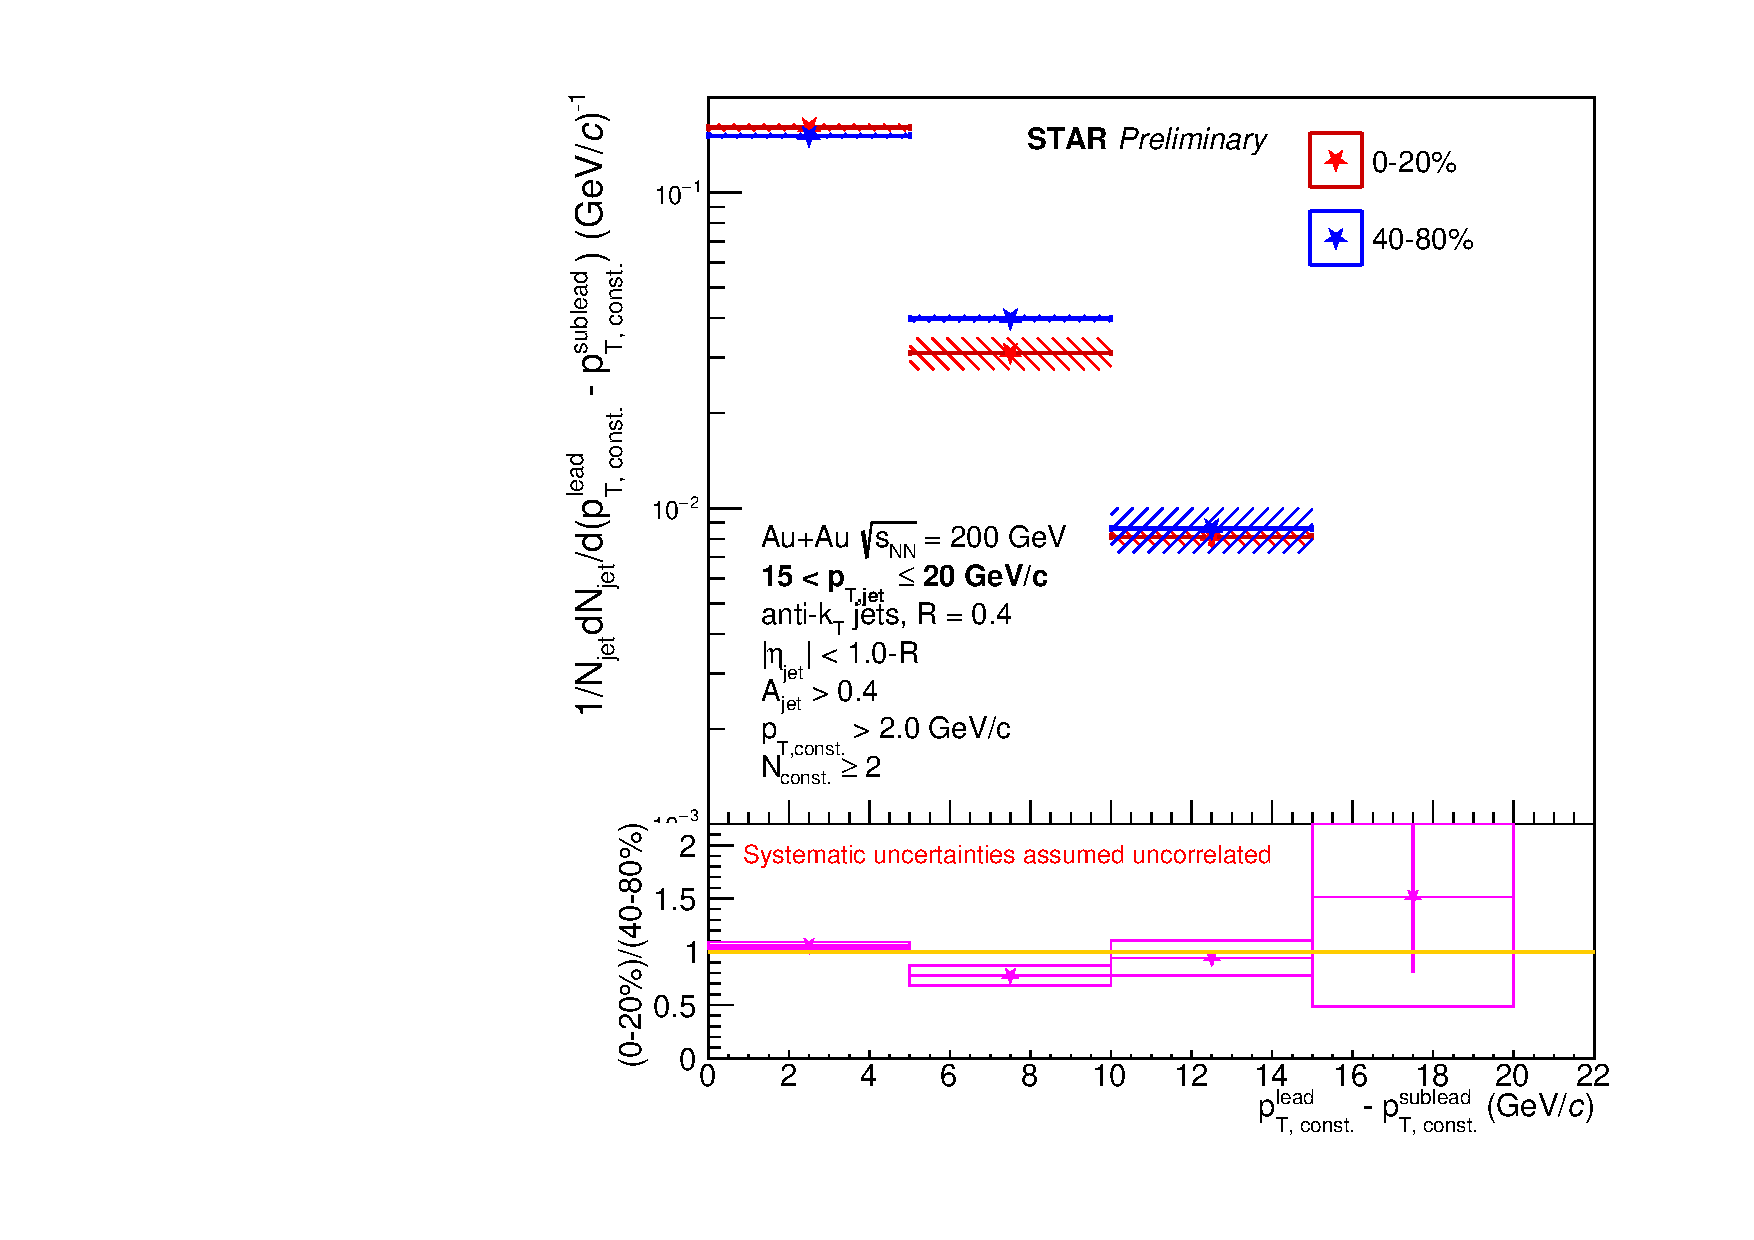
\includegraphics[width=0.32\linewidth]{angularities/AuAu/finalPlots_noPP_LeSub_0_v3_warn.pdf}
\end{frame}

\end{document}
